% \documentclass[oneside,12pt]{report} % ,twoside,draft,openright] % report e' per la tesi
\documentclass[11pt]{article}

\usepackage{setspace,graphicx,epstopdf,amsmath,amsfonts,amssymb,amsthm} %,versionPO}
\usepackage{marginnote,datetime,enumitem,subfigure,rotating,fancyvrb}
\usepackage{hyperref,float} % commenta se vuoi eiminare i link delle ref, vd sotto
\usepackage[longnamesfirst]{natbib}
\usdate

% hyperlink setup
\hypersetup{
	colorlinks=true,       % false: boxed links; true: colored links
	linkcolor=red,          % color of internal links (change box color with linkbordercolor)
	citecolor=green,        % color of links to bibliography
	filecolor=magenta,      % color of file links
	urlcolor=cyan           % color of external links
%, 	hidelinks		        % hide links (removing color and border)
}

% Save original definition of \marginpar
\let\oldmarginpar\marginpar

% Workaround for todonotes problem with natbib (To Do list title comes out wrong)
\makeatletter\let\chapter\@undefined\makeatother % Undefine \chapter for todonotes

% Define note commands
\newcommand{\smalltodo}[2][] {\todo[caption={#2}, size=\scriptsize, fancyline, #1] {\begin{spacing}{.5}#2\end{spacing}}}
\newcommand{\rhs}[2][]{\smalltodo[color=green!30,#1]{{\bf RS:} #2}}
\newcommand{\rhsnolist}[2][]{\smalltodo[nolist,color=green!30,#1]{{\bf RS:} #2}}
\newcommand{\rhsfn}[2][]{%  To be used in footnotes (and in floats)
\renewcommand{\marginpar}{\marginnote}%
\smalltodo[color=green!30,#1]{{\bf RS:} #2}%
\renewcommand{\marginpar}{\oldmarginpar}}
%\newcommand{\textnote}[1]{\ifnotes{{\noindent\color{red}#1}}{}}
\newcommand{\textnote}[1]{\ifnotes{{\colorbox{yellow}{{\color{red}#1}}}}{}}

% Command to start a new page, starting on odd-numbered page if twoside option 
% is selected above
\newcommand{\clearRHS}{\clearpage\thispagestyle{empty}\cleardoublepage\thispagestyle{plain}}

% Number paragraphs and subparagraphs and include them in TOC
\setcounter{tocdepth}{2}

% Nel caso non voglia alcun indentation con un nuovo paragrafo 
% \setlength{\parindent}{0pt}

% JFE-specific includes:
\usepackage{indentfirst} % Indent first sentence of a new section.
%\usepackage{jfe}          

% JFE-specific formatting of sections, etc.
% Theorems and the like
\newtheorem{theorem}{Theorem}[section]
\newtheorem{assumption}{Assumption}[section]
\newtheorem{proposition}{Proposition}
\newtheorem{conjecture}{Conjecture}
\newtheorem{lemma}{Lemma}[section]
\newtheorem{corollary}{Corollary}
\newtheorem{condition}{Condition}

%%%%%%%%%%%%%%%%%%%%%%%%%%%%%
%%%  to insert Python code: use 'listings' package
\usepackage{color}
\usepackage{listings}

\definecolor{Code}{rgb}{0,0,0}
\definecolor{Decorators}{rgb}{0.5,0.5,0.5}
\definecolor{Numbers}{rgb}{0.5,0,0}
\definecolor{MatchingBrackets}{rgb}{0.25,0.5,0.5}
\definecolor{Keywords}{rgb}{0,0,1}
\definecolor{self}{rgb}{0,0,0}
\definecolor{Strings}{rgb}{0,0.63,0}
\definecolor{Comments}{rgb}{0,0.63,1}
\definecolor{Backquotes}{rgb}{0,0,0}
\definecolor{Classname}{rgb}{0,0,0}
\definecolor{FunctionName}{rgb}{0,0,0}
\definecolor{Operators}{rgb}{0,0,0}
\definecolor{Background}{rgb}{0.98,0.98,0.98}

% \lstdefinelanguage{Python}{     % for defining more languages...
\lstset{language = Python,
	numbers=none,  % =left or =none
	numberstyle=\footnotesize,
	numbersep=1em,
	xleftmargin=1em,
	framextopmargin=2em,
	framexbottommargin=2em,
	showspaces=false,
	showtabs=false,
	showstringspaces=false,
	frame=l, % =l or = tb
	tabsize=4, 
	% Basic
	basicstyle=\ttfamily\footnotesize\setstretch{1},  % \ttfamily\small\setstretch{1},
	backgroundcolor=\color{Background},
	% Comments
	commentstyle=\color{Comments}\slshape,
	% Strings
	stringstyle=\color{Strings},
	morecomment=[s][\color{Strings}]{"""}{"""},
	morecomment=[s][\color{Strings}]{'''}{'''},
	% keywords
	morekeywords={import,from,class,def,for,while,if,is,in,elif,else,not,and,or,print,break,continue,return,True,False,None,access,as,,del,except,exec,finally,global,import,lambda,pass,print,raise,try,assert},
	keywordstyle={\color{Keywords}\bfseries},
	% additional keywords
	morekeywords={[2]@invariant,pylab,numpy,np,scipy},
	keywordstyle={[2]\color{Decorators}\slshape},
	emph={self},
	emphstyle={\color{self}\slshape},
}
% you can load code from file: \lstinputlisting{source.py}
%%%
%%%%%%%%%%%%%%%%%%%%%%%%%%%%%

%%%%%%%%%%%%%%%%%%%%%%%%%%%%%%%%%%%%%%%%%%%%%%%%%%%%%%%%%%%%%%%%%%%%%%%%%%%
%%%%%%%%%%%%%%%%      end of preamble and start of document     %%%%%%%%%%%
%%%%%%%%%%%%%%%%%%%%%%%%%%%%%%%%%%%%%%%%%%%%%%%%%%%%%%%%%%%%%%%%%%%%%%%%%%%
\begin{document}

%%%%%%%%%%%%%%%%%%%%%%%%%%%%%%%%%%%%%%%%%%%%%%%%%%%%%%%%%%%%%%%%%%%%%%%%%%%

\setlist{noitemsep}  % Reduce space between list items (itemize, enumerate, etc.)
%\onehalfspacing      % Use 1.5 spacing
% Use endnotes instead of footnotes - redefine \footnote command

\title{REVIEW NOTES: \\
	Data Science and Machine Learning    
	%\footnotetext{We gratefully acknowledge the inputs of Dom and \ldots} 
	}


\author{AM % \\ my_email
        }

\date{January 2018}  % First draft: November 2016             

% Create title page with no page number

\renewcommand{\thefootnote}{\fnsymbol{footnote}}   

\singlespacing

\maketitle

\vspace{-.2in}
\begin{abstract}
\noindent These are review notes on data science and machine learning based on various sources for my own consumption. It helps me refresh things I read, but they cannot be a substitute for a good book or tutorial.

\centering\textit{Use it at your risk: still full of typos and unfinished.} 
\end{abstract}

\medskip

\noindent \textit{JEL classification}: XXX, YYY.

\medskip
\noindent \textit{Keywords}: Python, learning algorithms %\LaTeX

\clearpage

\tableofcontents

\thispagestyle{empty}

\clearpage

%%%%%%%%%%%%%%%%%%%%%%%%%%%%%%%%%%%%%%%%%%%%%%%%%%%%%%%%%%%%%%%%%%%%%%%%%%%
\onehalfspacing
\setcounter{footnote}{0}
\renewcommand{\thefootnote}{\arabic{footnote}}
\setcounter{page}{1}
%%%%%%%%%%%%%%%%%%%%%%%%%%%%%%%%%%%%%%%%%%%%%%%%%%%%%%%%%%%%%%%%%%%%%%%%%%%
%%%%%%%%%%%%%%%%%%%%%%%%%%%%%%%%%%%%%%%%%%%%%%%%%%%%%%%%%%%%%%%%%%%%%%%%%%%
%\section*{Introduction}
The following notes are part of my review of machine learning. Code snippets are taken from various sources, online courses, stackoverflow and books. 

%%%%%%%%%%%%%%%%%%%%%%%%%%%%%%%%%%%%%%%%%%%%%%%%%%%%%%
%	DATA ANALYSIS
%%%%%%%%%%%%%%%%%%%%%%%%%%%%%%%%%%%%%%%%%%%%%%%%%%%%%%
\section{Data Analysis} \label{sec:Data}
First section is a crush course in two types of libraries: one for handling data (Numpy and Pandas) and one for visualisation (Matplotlib and Seaborn)

%%%%%%%%%%%%%%%%%%%%%%%%%%%%%%%%%%%%%%%%%%%%%%%%%%%%%%
\subsection{NumPy}
Numpy is the Python library for \textbf{linear algebra} (vectors and matrices) on which most useful libraries are built on (e.g. Pandas, SciPy,  Ski-learn, \ldots). It is fast since bound to C libraries.

\begin{lstlisting}
 import numpy as np   # using NumPy  
\end{lstlisting}

%%%%%%%%%%%%%%%%%%%%%
\subsubsection{Numpy Array}
Arrays come in two flavours: vectors (1-dim arrays) or matrices (2-dim arrays). The following shows a few methods and a couple of attributes.

\begin{lstlisting}
my_array = np.array([1,2,3])  # convert list into an array... 
# ... and list of lists ..., note extra []
my_matrix = np.array([[1,2,3], [4,5,6]])  

np.arange(start, end, step) # return value ranges 

np.zeros(3)  # 1-dim array of 3 zeros
np.zeros((3,4)) # matrix (2-dim array) of 3 x 4 zeroes, note extra ()
np.ones((3,4))  # matrix of 3 x 4 of ones

np.linspace(start, end, no_of_points)  # rtrn evenly-spaced values

np.eye(3) # identity matrix 3 x 3

np.random.rand(5) # random no. in (0,1) 
np.random.rand(5,5) # two-dim of random no.
np.random.randn(3) # 3 std Gaussian random no., note final 'n'
np.random.randint(low, higher, no_of_num) # rnd int in (low, high)
np.random.seed(101)  # seed for reproducing results

my_array.reshape(4,4) # reshape an array in a matrix 4x4

my_arr.max()  # return max value, similarly for min

my_arr.argmax()  # return index location of max value
# for df NB: df.idxmax # rtrn idx across df series

my_arr.shape  # diplay an array dimension (NB: attribute, not method)
my_arr.dtype  # display data type (e.g. int32)
\end{lstlisting}

%%%%%%%%%%%%%%%%%%%%%
\subsubsection{Numpy array Indexing}
How to select elements in an array (also using boolean conditions).

\begin{lstlisting}
my_array[5]  # return value at index 5 (start at 0, as per lists)
my_array[0:5]  # return values in a range (1st included, last not)
 
my_array[0:5] = 1.0  # change values in a list (i.e. broadcasting)
new_array = my_array[0:5]  # create slice
new_array[:] = 5  # NB: changes affect also original array 
            # (i.e. my_array), this is to avoid memory issues.  
arr_copy = my_array.copy()   # but you can create copy explicitly 

arr_2d[row][col]  # indexing of 2-dim array
arr_2d[row,col]   # same as above
arr_2d[:2,1:]     # 2-dim array slicing
arr_2d.shape[1]   # shape of 2nd dim, NB: diff vs. 1-dim above
arr_2d[[1,4,5]]   # fancy indexing: row 1, 4, and 5; note [[]]

bool_arr = my_arr > 4  # returns an array of True or False 
                       # (condition checked for each element)
new_arr[bool_arr]  # return array with those elements 
                   # for which condition true
new_arr[my_arr > 4]  # same as above
\end{lstlisting}

%%%%%%%%%%%%%%%%%%%%%
\subsubsection{Numpy operations}
How to perform operations.
\begin{lstlisting}
arr_sum = arr_first + arr_second  # sum element by element
                                 # similarly for '-', '*', '/'
np.sqrt(arr); np.exp(arr); ... # standard math functions
\end{lstlisting}
Note that in case of division by zero, there will not be any error msg (just warnings) and \textbf{nan} will be returned. Similarly, in case operations return infinity (e.g. +/- something/0), one gets just warnings and a +/-\textbf{inf} result.


%%%%%%%%%%%%%%%%%%%%%%%%%%%%%%%%%%%%%%%%%%%%%%%%%%%%%%
\subsection{Pandas}
One can think of Pandas as a powerful Excel version to read and manipulate data.
\begin{lstlisting}
import numpy as np
import pandas as pd
\end{lstlisting}

\subsubsection{Series}
This is a data type of Pandas similar to a NumPy array (built, indeed, on top of it), but with axis labels (i.e. \textbf{indexed by labels} besides number location) and can hold \textbf{any} Python \textbf{object} (not just numbers).
You can convert a list, array or dictionary to a Series. 
\begin{lstlisting}
my_list = [1,2,4]
labels = ['a','b','c']
pd.Series(data=my_list, index=labels) # convert list to a Series 
                                      #(here also indexed)
                                      # pd.Series(my_list, labels)   
dic = {'a':1,'b':2,'c':4}
pd.Series(dic)   # note: labels are the dict keys

pd.Series([sum, len, print])  # Series can hold any Python object
\end{lstlisting}

Pandas makes use of index names or numbers by allowing for fast look ups of information (works like a hash table or dictionary).
\begin{lstlisting}
ser1 = pd.Series([1,2,3,4],index=['USA', 'Ger','USSR', 'Japan'])     
ser1['USSR']   # returns 3
ser1 + ser2 # operations are based on index, if discrepancies 'NaN'
\end{lstlisting}

\subsubsection{DataFrames}
DataFrame is the workhorse of pandas (inspired by R language), akin to a \textbf{bunch of Series} that share \textbf{same index}.
\begin{lstlisting}
df = pd.DataFrame(randn(5,4), 
                  index='A B C D E'.split(), 
                  columns='W X Y Z'.split()) # table 5x4
                  
# create a dataframe from lists (Day and Month are columns name)
df = pd.DataFrame({'Day': [31, 30, 31, 30], 'Month': ['Jan', 'Apr', 'Mar', 'June']})
\end{lstlisting}

There are various methods to get data (note that DataFrames columns are just Series, try type() fnct).
\begin{lstlisting}
df['W']  # get column of above table; df.W works too (but avoid!)
df[['W','Z']] # get two columns; NB: [[]]

df.drop('X',axis=1) # remove column X, temporarily 
                    # (df still as before, if called)
df.drop('X',axis=1, inplace=True) # remove column, permanently
                             # NB: inplace use here and later
df.drop('E',axis=0) # this is to remove row; note axis value

df.loc['A']  # select a row using labels. NB: []
	   #inputs: label, labels list or slices, boolean array, callabe fnct
df.iloc[2] # select a row using position (instead of labels)
	   # inputs: integers, list of int, slices of int, boolean array
df.ix['A'] # primarily label based, but will fall back to position
           # (deprecated from 2017)

df.iloc[0:5] # first five rows of dataframe
df.iloc[[0,3,6], [0,5,6]] # 1st, 4th, 7th rows + 1st 6th 7th columns.

type(df['col'].iloc[0]) # to get a datatype, e.g 'str'


df.loc['B','Y'] # selected subset of row and column (one value here)
df.loc[['A','B'],['W','Y']] # a table of 2x2 here

df[df>0]  # conditional selection (nb: possible NaN); like numpy array
df[df['W']>0]  # another example, NB: look inside[]: a Series
df[df['W']>0][['Y','X']]  # but returning only two columns
df[(df['W']>0) & (df['Y'] > 1)]  # two conditions 
                          # one can use | and & with ()
\end{lstlisting}

Index manipulation:
\begin{lstlisting}
df.reset_index()  # reset to default index: 0, 1, ... , n

df['States'] = 'CA NY WY OR CO'.split()  # add a new Series
df.set_index('States')  # make 'States' the new index
df.set_index('States', inplace=True)  # use inplace (permanent)

# multi-index
outside = ['G1','G1','G1','G2','G2','G2']
inside = [1,2,3,1,2,3]
hier_index = list(zip(outside,inside))
hier_index = pd.MultiIndex.from_tuples(hier_index)
df = pd.DataFrame(np.random.randn(6,2),
                  index=hier_index,
                  columns=['A','B'])
df.loc['G1'].loc[1]
df.index.names = ['Group','Num']
df.xs(['G1',1])  # cross-section grab, see more below
df.xs(1,level='Num')
\end{lstlisting}

\subsubsection{Missing data} \label{missing_data_pandas}

Examples to deal with the very common issue of missing data.
\begin{lstlisting}
df = pd.DataFrame({'A':[1,2,np.nan], 
                   'B':[5,np.nan,np.nan],
                   'C':[1,2,3]})

df.dropna()  # remove rows where NaN
df.dropna(axis=1) # remove column where NaN

df.dropna(thresh=2)  #  remove rows where NaN >= 2

df.fillna(value='FILL') # insert 'FILL' where NaN
# df=df.fillna(0)
df['A'].fillna(value=df['A'].mean()) # insert col mean where NaN 
df.fillna(method='ffill', limit=1)  # fill forward, to 1 next only
\end{lstlisting}

\subsubsection{Groupby}
The 'groupby' method allows to 1. group rows of data together in order to 2. call aggregate functions:
\begin{lstlisting}
# Create dataframe
data = {'Company':['GOOG','GOOG','MSFT','MSFT','FB','FB'],
        'Person':['Sam','Charlie','Amy','Vanessa','Carl','Sarah'],
        'Sales':[200,120,340,124,243,350]}
df = pd.DataFrame(data)

by_comp = df.groupby("Company") # group rows together of 
                          # a column name , here 'Company'
by_comp.mean()  # call aggregate method: rtrn table with mean 
                # for each company
                # e.g.  .std .max() .count() .describe() ...
                
# or, better,
byMonth = df.groupby('Month').count()
byMonth.head()  # to display

# group by two variables (multi-idx), then unstuck() (2nd var -> col)
df.groupby(by=['Day of Week','Hour']).count()['Reason'].unstack()

# NB: difference between above and following call 
df[df['Reason']=='Traffic'].groupby('Date').count()['lat']
\end{lstlisting}

\subsubsection{Merging, joining and concatenating}
There are 3 main ways to combine DataFrames together: merging, joining and concatenating.
\begin{lstlisting}
pd.concat([df1,df2,df3])  # glue together DataFrames along axis 
                          # (here index, axis=0 by default)
pd.concat([df1,df2,df3], axis=1)  # glue together along columns
bank_stocks = pd.concat([BAC,C], axis=1,keys=['BAC','C']) 
									    # multi-hier. cols
bank_stocks.columns.names =['Banc tkr', 'stock prices/vol']

bank_stocks['BAC']['Close']  # close prices series for just BAC
## or close prices series for all stocks (e.g. to make plot)
bank_stocks.xs(key='Close',axis=1, level='stock prices/vol') 

df = pd.merge(df, movies_titles, on = 'item_id') # add titles
pd.merge(left,right,how='inner',on='key')  # logic similar to SQL, 
                                  #  how='outer' ='right' ='left'
pd.merge(left, right, on=['key1', 'key2']) # more complicated example

left.join(right)    # combining columns of differently-indexed DF
left.join(right, how='outer')  # different result
\end{lstlisting}

\subsubsection{Operations}
Some examples of more operations:
\begin{lstlisting}
df.head()
df.tail()

df['col2'].unique()  # show unique values
df['col2'].nunique() # no. of unique values (one value)
df['col2'].value_counts()  # count no. same value appears
df['col2'].value_counts().head() # top 5

def times2(x): 
       return x*2
df['col1'].apply(times2)  # apply fnct to each element
df['col1'].apply(lambda x: x*2)  # similar

# How many people have the word Chief in their job title? (tricky)
def chief_string(title):
	if 'chief' in title.lower():
		return True
	else:
		return False
sum(sal['JobTitle'].apply(lambda x: chief_string(x)))

del df['col1']  # another way to remove permanently a column
df.columns  # columns names
df.index 

# sort - note: inplace=false by default
df.sort_values(by='col2', ascending=False)  

df.isnull()  # boolean: find null values, return True/False

df.pivot_table(values='D',index=['A', 'B'],columns=['C'])

df['timeStamp'] = pd.to_datetime(df['timeStamp'])   # from str to datetime
df['Hour'] = df['timeStamp'].apply(lambda time: time.hour)

# timezones
import pytz
data = data.tz_localize(pytz.timezone('US/Eastern')) # specify current tz
data = data.tz_convert(pytz.timezone('GMT'))  # convert to another tz
\end{lstlisting}

\subsubsection{Data input and output} 
Pandas offers a variety of way to read or output files:
\begin{lstlisting}
df = pd.read_csv('example')  # CSV input
df = pd.to_csv('example', index=False)  # CSV output

# works also for Excel data (not images or macro)            
pd.read_excel('excel_sample.xlsx', sheet_name='Sheet1') 
# for output, similarly, pd.to_excel(...)

# to read HTML you need following libraries (e.g. conda): 
#      lxml,BeautifulSoup4
df = pd.read_html('http://www.fdic.gov/[...]/banklist.html')  
# read tables off of a webpage and return a list of DataFrame objects
df[0]  # shows table of failed banks...
\end{lstlisting}

%%%%%%%%%%%%%%%%%%%%%%%%%%%%%%%%%%%%%%%%%%%%%%%%%%%%%%
\subsubsection{Built-in visualisation}
Built-off of matplotlib, in Pandas for easy of use.

Matplotlib has style sheets you can use to make your plots look a little nicer. These style sheets include 'bmh', 'fivethirtyeight', 'ggplot', 'dark\_background' and more. Some example below.

\begin{lstlisting}
df1['A'].hist() # hist before any style

# call the style and plot with the style
import matplotlib.pyplot as plt
plt.style.use('ggplot')
df1['A'].hist()
\end{lstlisting}

There are several built-in plot types in pandas. Some examples below:
\begin{lstlisting}
df2.plot.area(alpha=0.4)  # note transparency param
df2.plot.bar(stacked=True)
df1['A'].plot.hist(bins=50, alpha=0.5, label="X")
df1.plot.line(x=df1.index,y='B',figsize=(12,3),lw=1)
df1.plot.scatter(x='A',y='B')

df = pd.DataFrame(np.random.randn(1000, 2), columns=['a', 'b'])
df.plot.hexbin(x='a',y='b',gridsize=25,cmap='Oranges')

df2.plot.box() # Can also pass a by= argument for groupby
df2['a'].plot.kde()

df2.plot.density() # more
\end{lstlisting}


%%%%%%%%%%%%%%%%%%%%%%%%%%%%%%%%%%%%%%%%%%%%%%%%%%%%%%
\subsection{SciPy}
SciPy is a collection of math algorithms and useful functions built on NumPy. It makes Python a data processing system rivalling MatLab, Octave, R, etc.

Scientific applications using SciPy benefit from the additional modules in numerous niches: everything from parallel programming, web and data-base subroutines, and classes.

Some examples in linear algebra:
\begin{lstlisting}
import numpy as np
A = np.array([[1,2,3],[4,5,6],[7,8,8]])  # matrix

from scipy import linalg  # get relevant module
linalg.det(A)  # compute determinant of a matrix
P, L, U = linalg.lu(A)  # get matrix decomposition
EigenW, EigenV = linalg.eig(A)  # eigen vectors and values
linalg.solve(A,v) # solve systems of linear eq.
\end{lstlisting}


%%%%%%%%%%%%%%%%%%%%%%%%%%%%%%%%%%%%%%%%%%%%%%%%%%%%%%
\subsection{Matplotlib}
Created by John Hunter to replicate MatLab'plotting in Python. You can see examples/gallery with \textbf{code} to copy in the official webpage: http://matplotlib.org/.
\begin{lstlisting}
import matplotlib.pyplot as plt
%matplotlib inline  # once for notebooks only, 
                  # otherwise plt.show() each time
\end{lstlisting}

%%%%%%%%%%%%%%%%%%%%%%%%%%%%%%%%%%%%%%%%%%%%%%%%%%%%%%
\subsubsection{Basic}
Two ways to use it: simple way or object-oriented API (i.e. instantiate fig obects and then call methods). Second is more flexible and recommended for multiplots.

\begin{lstlisting}
####################
# Simpler way

# 1a. simple line plot
plt.plot(x, y, 'r')  # 'r' is the red colour
plt.xlabel('X label here')
plt.ylabel('Y label here')
plt.show()

# 2a. multiplots on same canvas (next)
plt.subplot(1,2,1)  # (no_rows, no_columns, plot_no)
plt.plot(x,y,'--r')
plt.subplot(1,2,2)
plt.plot(x,y, 'g*-')


####################
# Object oriented way

# 1b. simple line plot
fig = plt.figure() # create empty canvas
# then add axes: left, bottom, width, height (0 to 1)
axes =  fig.add_axes([0.1,0.1,0.8,0.8]) 
# plot
axes.plot(x,y,'b')
axes.set_xlabel('Set X Label') # NB: 'set_' 
axes.set_ylabel('Set y Label')
axes.set_title('Set Title') # method for setting titles


# 2b. multiplots on same canvas (one inset)
fig = plt.figure()
axes1 = fig.add_axes([0.1, 0.1, 0.8, 0.8]) # main axes
axes2 = fig.add_axes([0.2, 0.5, 0.4, 0.3]) # inset axes

# Larger Figure Axes 1
axes1.plot(x, y, 'b')
axes1.set_xlabel('X_label_axes2')
axes1.set_ylabel('Y_label_axes2')
axes1.set_title('Axes 2 Title')

# Insert Figure Axes 2
axes2.plot(y, x, 'r')
axes2.set_xlabel('X_label_axes2')
axes2.set_ylabel('Y_label_axes2')
axes2.set_title('Axes 2 Title') 
fig

# 2c. multiplots on same canvas (next)
# Empty canvas of 1 by 2 subplots
fig, axes = plt.subplots(nrows=1, ncols=2)  # unpacking

for ax in axes:  # NB: ax[0] and ax[1]
	ax.plot(x, y, 'b')
	ax.set_xlabel('x')
	ax.set_ylabel('y')
	ax.set_title('title')

# another example of unpacking (NB: vs above)
f, (ax1, ax2) = plt.subplots(1, 2, sharey=True,figsize=(10,6))
	
fig # Display the figure object 
fig.tight_layout() # or plt.tight_layout() to adjust overlapping   

# figsize(width, height), dpi is dots-per-inch (pixel)
fig = plt.figure(figsize=(8,4), dpi=100)


# output in PNG, JPG, EPS, SVG, PGF, PDF, ...
fig.savefig("filename.png", dpi=200) # save fig, dpi optional

# adding legend: label='label txt'
ax.plot(x, x**3, label="x**3")
ax.legend()
# and its position
ax.legend(loc=1) # upper right corner
ax.legend(loc=2) # upper left corner
ax.legend(loc=3) # lower left corner
ax.legend(loc=4) # lower right corner
ax.legend(loc=0) # let matplotlib decide best
# or just outside upper corner
plt.legend(bbox_to_anchor=(1.05, 1), loc=2, borderaxespad=0.)

# colours: by name or RGB hex code
ax.plot(x, x+1, color="blue", alpha=0.5) # half-transparant
ax.plot(x, x+2, color="#8B008B")        # RGB hex code
ax.plot(x, x+3, color="#FF8C00")        # RGB hex code 

# linewidth or lw (0.25... 3) and 
# linestyle or ls: "-", "-.", ":", "steps"
# marker = '+', 'o', '*', 's', ',', '.', '1', '2', '3', '4', ...
ax.plot(x, x+5, color="green", linewidth=3, linestyle='-')
ax.plot(x, x+6, color="green", lw=3, ls='-.')
ax.plot(x, x+13, color="purple", lw=1, ls='-', 
        marker='o', markersize=2)

# set_ylim and set_xlim methods in the axis object
axes[0].set_ylim([0, 60])
axes[0].set_xlim([2, 5])

# barplots, histograms, scatter plots, and much more.
plt.scatter(x,y)
plt.hist(random.sample(range(1, 1000), 100))
data = [np.random.normal(0, std, 100) for std in range(1, 4)]
plt.boxplot(data,vert=True,patch_artist=True); 
\end{lstlisting}

%%%%%%%%%%%%%%%%%%%%%%%%%%%%%%%%%%%%%%%%%%%%%%%%%%%%%%
\subsubsection{Advanced}
Some more:
\begin{lstlisting}
axes[1].set_yscale("log") # add logarithm scale
ax.set_xticks([1, 2, 3, 4, 5]) # or set_yticks, [] where ticks placed
ax.set_xticklabels([r'$\alpha$', r'$\beta$', r'$\gamma$', 
            r'$\delta$', r'$\epsilon$'], fontsize=18)

# distance between x and y axis and the numbers on the axes
matplotlib.rcParams['xtick.major.pad'] = 5  # = 3 default
matplotlib.rcParams['ytick.major.pad'] = 5

# when saving figures the labels are sometimes clipped, 
# and it can be necessary to adjust the positions of axes
fig.subplots_adjust(left=0.15, right=.9, bottom=0.1, top=0.9)

axes[0].grid(True)
axes[1].grid(color='b', alpha=0.5, linestyle='dashed', linewidth=0.5)


ax.spines['bottom'].set_color('blue')
ax.spines['top'].set_color('blue')
ax.spines['left'].set_color('red')
ax.spines['left'].set_linewidth(2)

fig, ax = plt.subplots()

cnt = ax.contour(Z, cmap=matplotlib.cm.RdBu, vmin=abs(Z).min(), 
				 vmax=abs(Z).max(), extent=[0, 1, 0, 1])

# ... and much more ... look at the matplotlib gallery
\end{lstlisting}

%%%%%%%%%%%%%%%%%%%%%%%%%%%%%%%%%%%%%%%%%%%%%%%%%%%%%%
\subsection{Seaborn}
Seaborn is a library for making attractive and informative statistical graphics in Python. It is built on top of matplotlib and tightly integrated with the PyData stack (incl. support for numpy and pandas data structures and statistical routines from scipy and statsmodels).

Check gallery at http://seaborn.pydata.org/
\begin{lstlisting}
import seaborn as sns
%matplotlib inline # for notebooks only
\end{lstlisting}


%%%%%%%%%%%%%%%%%%%%%%%%%%%%%%%%%%%%%%%%%%%%%%%%%%%%%%
\subsubsection{Distribution plots}
We look at 5 different distribution plots:
\begin{lstlisting}
tips = sns.load_dataset('tips') # sns comes with built-in datasets
tips.head() # pandas dataframes

# 1. for uni-variate distribution
sns.distplot(tips['total_bill']) # NB: Series
sns.distplot(tips["total_bill"],kde=False,bins=30) # with some params

# 2. for bi-variate data (NB: how two variables expressed)
sns.jointplot(x="total_bill",y="tip",data=tips,kind="scatter")
# or kind= "scatter”, “reg”, “resid”, 'kde', 'hex'

# 3. pairwise relationships (table of dists)
sns.pairplot(tips)  # NB: all Dataframe
sns.pairplot(tips,hue='sex',palette='coolwarm') # NB: hue support

# 4. for uni-variate distr: dash marks for every point 
sns.rugplot(tips['total_bill'])

# 5. kdeplots are Kernel Density Estimation plots
sns.kdeplot(tips['total_bill']) # or
sns.kdeplot(df['col1'], df['col2'])  # for bi-variate
\end{lstlisting}

%%%%%%%%%%%%%%%%%%%%%%%%%%%%%%%%%%%%%%%%%%%%%%%%%%%%%%
\subsubsection{Categorical plots}
Below there are 6 example plots for categorical (i.e. non-numerical) data.
\begin{lstlisting}
# 1. & 2. aggregate categorical data
sns.barplot(x='sex',y='total_bill',data=tips) # by default y=mean(y)
sns.barplot(x='sex',y='total_bill',data=tips,estimator=np.std) #NB:std
sns.countplot(x='sex',data=tips) # like barplot but y = count of x

# 3 & 4. distribution of categorical data
sns.boxplot(x="day", y="total_bill", data=tips,palette='rainbow')
sns.boxplot(data=tips,palette='rainbow',orient='h') # NB: entire df
sns.boxplot(x="day", y="total_bill", hue="smoker",data=tips,
            palette="coolwarm")
sns.violinplot(x="day", y="total_bill", data=tips,palette='rainbow')
sns.violinplot(x="day", y="total_bill", data=tips,
               hue='sex',palette='Set1') # hue
sns.violinplot(x="day", y="total_bill", data=tips,hue='sex',
                split=True,palette='Set1') # split hue

# 5 & 6. draw scatter where one variable is categorical
sns.stripplot(x="day", y="total_bill", data=tips)
sns.stripplot(x="day", y="total_bill", data=tips,
              jitter=True, hue='sex',split=True)
# swarmplot is similar to stripplot(), but points adjusted 
# (only along the categorical axis) so that they do not overlap
sns.swarmplot(x="day", y="total_bill", data=tips)
sns.swarmplot(x="day", y="total_bill",
           hue='sex',data=tips, palette="Set1", split=True)

# combining categorial plots (swarmplot into violin, see below)
sns.violinplot(x="tip", y="day", data=tips,palette='rainbow')
sns.swarmplot(x="tip", y="day", data=tips,color='black',size=3)

# factorplot is the most general form of a categorical plot 
# it can take in a kind parameter to adjust the plot type:
sns.factorplot(x='sex',y='total_bill',data=tips,kind='bar') #barplot
\end{lstlisting}

%%%%%%%%%%%%%%%%%%%%%%%%%%%%%%%%%%%%%%%%%%%%%%%%%%%%%%
\subsubsection{Matrix plots}
Matrix plots is basically a \textbf{heatmap} for correlations or similar numbers (or \textbf{clustermap}: clustered heatmap).
\begin{lstlisting}
tips.corr() # matrix of correl
sns.heatmap(tips.corr()) # matrix of corr by colour
sns.heatmap(tips.corr(),cmap='coolwarm',annot=True) # NB annot inside

flights = sns.load_dataset('flights')
flights.pivot_table(values='passengers',index='month',columns='year')
sns.heatmap(pvflights,cmap='magma',linecolor='white',linewidth=1) 

sns.clustermap(pvflights) # months/years grouped by similarities
sns.clustermap(pvflights,cmap='coolwarm',standard_scale=1) 
\end{lstlisting}

%%%%%%%%%%%%%%%%%%%%%%%%%%%%%%%%%%%%%%%%%%%%%%%%%%%%%%
\subsubsection{Regression plots}
There are many in-built capabilities for regression, here we only show \textbf{lmplot()}
\begin{lstlisting}
# chart with points and fitted regression (and stdev overlaid)
# NB: can be an alternative to plt.scatter with 'fit_reg=False'
sns.lmplot(x='tota_bill',y='tip',data=tips)
sns.lmplot(x='total_bill',y='tip',data=tips,hue='sex')
sns.lmplot(x='total_bill',y='tip',data=tips,hue='sex',
       palette='coolwarm', markers=['o','v'],
       scatter_kws={'s':100}) # last is squared markersize

# two charts next, one for male and one for female
sns.lmplot(x='total_bill',y='tip',data=tips,col='sex')
# four charts - NB: row and col
sns.lmplot(x="total_bill", y="tip", row="sex", col="time",data=tips)
# using (..., fit_reg=False, ..) is like a scatter plot (ie no fit regression)

#  aspect and size
sns.lmplot(x='total_bill',y='tip',data=tips,col='day',
		hue='sex',palette='coolwarm', order=1
        aspect=0.6,size=8)
        
# NB: here x and y variables can be also pd.Series, np.arrays, besides str
# hence no need of data=
sns.regplot(x=advertising['TV'], y=advertising['Sales'], order=1,
            scatter_kws={'color':'red'}, ci=None) 
\end{lstlisting}

%%%%%%%%%%%%%%%%%%%%%%%%%%%%%%%%%%%%%%%%%%%%%%%%%%%%%%
\subsubsection{Grids}
Grids (PairGrid, JoinGrid, and the more general FacetGrid) are generic types of plots that allow to map different plot types to rows and columns of a grid.
\begin{lstlisting}
iris = sns.load_dataset('iris')

# 1. Pairgrid is a general version of pairplot() type grids
g = sns.PairGrid(iris) # Just an empty PairGrid
g.map(plt.scatter) # then map scatter to all

# Map to upper,lower, and diagonal
g = sns.PairGrid(iris)
g.map_diag(plt.hist)  # NB: _diag, _upper, _lower
g.map_upper(plt.scatter)
g.map_lower(sns.kdeplot) # NB: sns. 

# NB: pairplot-> hist mapped on diagonal & scatter everywhere else

# 2. JointGrid is the general version for jointplot() type grids
g = sns.JointGrid(x="total_bill", y="tip", data=tips)
g = g.plot(sns.regplot, sns.distplot)

# 3. FacetGrid is the GENERAL way to create grids 2x2
g = sns.FacetGrid(tips, col="time", row="smoker") # empty Grid
g = g.map(plt.hist, "total_bill")

g = sns.FacetGrid(tips, col="time", row="smoker",hue='sex') # hue
# Notice two arguments after plt.scatter call
g = g.map(plt.scatter, "total_bill", "tip").add_legend()

# FacetGrid 1x2
g = sns.FacetGrid(data=titanic,col='sex')
g.map(plt.hist,'age') # x =  age, y = male, female

# FacetGrid histogram with hue
g = sns.FacetGrid(df,hue="Private",
				palette='coolwarm',size=6,aspect=2)
g = g.map(plt.hist,'Grad.Rate',
				bins=20,alpha=0.7) # hue overlapping hist
\end{lstlisting}

%%%%%%%%%%%%%%%%%%%%%%%%%%%%%%%%%%%%%%%%%%%%%%%%%%%%%%
\subsubsection{Style and Colour}
\begin{lstlisting}
sns.set_style('white') # background colour
sns.set_style('whitegrid') # another
sns.set_style('ticks') # external ticks
sns.despine() # spine removal
sns.set_palette("GnBu_d") # grey colour


plt.figure(figsize=(12,3)) # can use this in sns to control size

sns.set_context('poster',font_scale=4) # allows overriding default
sns.countplot(x='sex',data=tips,palette='coolwarm') # no default-ones
\end{lstlisting}


%%%%%%%%%%%%%%%%%%%%%%%%%%%%%%%%%%%%%%%%%%%%%%%%%%%%%%
\subsection{Plotly and Cufflinks}
Plotly is a library that allows you to create \textbf{interactive} plots that you can use in dashboards or websites (you can save them as html files or static images) - check https://plot.ly/. 

Cufflinks instead links Plotly to Pandas (also check technical analysis library of Cufflinks, still in beta version - see github rep).

\begin{lstlisting}
# installation
pip install plotly # also via conda
pip install cufflinks
\end{lstlisting}

Set-up is the most complicated thing, then it works by just adding an 'i' to 'plot'.
\begin{lstlisting}
from plotly import __version__
from plotly.offline import download_plotlyjs, init_notebook_mode, 
                           plot, iplot
print(__version__) # requires version >= 1.9.0
import cufflinks as cf

init_notebook_mode(connected=True) # for notebooks
cf.go_offline() # for offline use
\end{lstlisting}

Let's create a couple of fake dataframes (5x4, 3x2, 3D) and ...
\begin{lstlisting}
df = pd.DataFrame(np.random.randn(100,4),columns='A B C D'.split())
df2 = pd.DataFrame({'Category':['A','B','C'],'Values':[32,43,50]})
df3 = pd.DataFrame({'x':[1,2,3,4,5],'y':[10,20,30,20,10],
		'z':[5,4,3,2,1]})
\end{lstlisting}
... let's explore Plotly functionality (double-click on pic to zoom out), by just adding an 'i' to 'plot' and specifying the 'kind' is all we need:
\begin{lstlisting}
# Scatter plots
df.iplot(kind='scatter',x='A',y='B',mode='markers',size=10) 

# Bar plots
df2.iplot(kind='bar',x='Category',y='Values')
df.count().iplot(kind='bar')

# Boxplots
df.iplot(kind='box') # click on relevant Series to show

# 3D surfaces
df3.iplot(kind='surface',colorscale='rdylbu')

# Spreads
df[['A','B']].iplot(kind='spread')

# Histogram
df['A'].iplot(kind='hist',bins=25)

# Bubble: e.g. GDP charts
df.iplot(kind='bubble',x='A',y='B',size='C')

# Similar to sns.pairplot()
df.scatter_matrix()
\end{lstlisting}

%%%%%%%%%%%%%%%%%%%%%%%%%%%%%%%%%%%%%%%%%%%%%%%%%%%%%%
\subsection{Example: finance nb}
Just a quick ref for finance nb:
\begin{lstlisting}
from pandas_datareader import data, wb
start = datetime.datetime(2006, 1, 1)
end = datetime.datetime(2016, 1, 1)
# CitiGroup
C = data.DataReader("C", 'google', start, end)
# ... more

# Could also do this for a Panel Object
df = data.DataReader(['BAC', 'C', 'GS', 'JPM', 'MS',
	 'WFC'],'google', start, end)

# otherwise
bank_stocks = pd.concat([BAC, C, GS, JPM, MS, WFC],
			axis=1,keys=tickers)  # NB axis and keys
bank_stocks.columns.names = ['Bank Ticker','Stock Info']
# using xc (multi-level indexing fnct)
bank_stocks.xs(key='Close',axis=1,level='Stock Info').max()

# get rtrns
returns = pd.DataFrame()  # get empty df
for tick in ['BAC', 'C', 'GS', 'JPM', 'MS', 'WFC']:  
	returns[tick+' Return'] = bank_stocks[tick]['Close'].pct_change()

# visualise
sns.pairplot(returns[1:])
returns.idxmin()  # when min daily rtrn
returns.std() # std dev for 6 rtrns series

# plot (2 ways for panel data: loop or .xs)
for tick in tickers:
	bank_stocks[tick]['Close'].plot(figsize=(12,4),label=tick)
# or alternative
bank_stocks.xs(key='Close',axis=1,level='Stock Info').plot()

# moving avg
plt.figure(figsize=(12,6))
BAC['Close'].ix['2008-01-01':'2009-01-01'].
		.rolling(window=30).mean().plot(label='30 Day Avg')
BAC['Close'].ix['2008-01-01':'2009-01-01'].plot(label='BAC CLOSE')
plt.legend()

# cluster
sns.clustermap(bank_stocks.xs(key='Close',axis=1,
			level='Stock Info').corr(),annot=True)
\end{lstlisting}

%%%%%%%%%%%%%%%%%%%%%%%%%%%%%%%%%%%%%%%%%%%%%%%%%%%%%%
%	MACHINE LEARNING
%%%%%%%%%%%%%%%%%%%%%%%%%%%%%%%%%%%%%%%%%%%%%%%%%%%%%%
\section{Machine Learning: an intro} \label{sec:Machine}
Machine learning is a method of data analysis that automates analytical model building, using algorithms that iteratively learn from data.

It is used for: fraud detection (unsupervised), recognised someone in a picture give some of its previous pics (supervised), customer segmentation, credit scoring, image recognition, sentiment analysis, etc.

There are three main kinds of machine learning:
\begin{itemize}
	\item \textbf{Supervised} learning: algorithms trained using inputs (also called features, attributes, independent variables, ...) with corresponding correct outputs (also called labels in classification, dependent variables, ...) that are used by the algo to learn by comparing forecasted vs. correct output to find errors and modify model accordingly. Commonly used for predictions; e.g. regression.
	\item \textbf{Unsupervised} learning: system does not have correct outputs as examples, aim is to \textbf{explore} data to find some structure within (segmenting the data); i.e. mainly clustering (sometimes called 'unsupervised classification', e.g. K-Means or DBSCAN\footnote{Indeed: in classification you have a set of predefined classes and want to know which class a new object belongs to; whilst in Clustering you try to group a set of objects to find whether there is some relationship between.}) or dimensionality reduction (e.g. PCA).
	\item \textbf{Reinforcement} learning: algorithm learns by trial and error which actions yields greatest rewards - mostly used in gaming (e.g. chess engine), navigation or robotics. Three main parts: agent (learner), environment (everything the agent interacts with) and actions (what the	agent can do) - the agent tries to maximize the reward by a series of actions/interactions with the environment.
\end{itemize}

To recap, the main elements are:
\begin{itemize}
	\item supervised learning: (i) label data / targets, (ii) direct feedback, (iii) predict outcome;
	\item unsupervised learning: (i) no labels, (ii) no feedback, (iii) find hidden structure in data;
	\item reinforcement learning: (i) decision process, (ii) reward system, (iii) learn series of actions.
\end{itemize}

For supervised learning, you can further distinguish between (supervised) \textbf{classification} and \textbf{regression}, respectively, in terms of (i) output types (NB: output and not inputs): discrete (class labels) vs. continuous (numbers), (ii) result: decision boundary vs. best fit line and (iii) evaluation: accuracy (precision, recall, etc.) vs. mse (r-squared, etc.).

Some (supervised) classification learning definitions: (i) instances (inputs / features): e.g. pictures, credit scores; (ii) concept: function that maps inputs and outputs; (iii) target concept: what we are trying to find (needs to be defined); (iv) hypothesis class: set of all concepts, of all possible functions (not regression like obviously); (v) sample (training set): set of all inputs paired with correct labels; (vi) candidate: concept that we think is the target concept (vii) testing set: inputs paired with correct labels on which to test the candidate. 

Using Scikit Learn in Python, main steps (uniform interface across methods):
\begin{lstlisting}
conda install scikit-learn # installation

# every algorithm exposed via an 'estimator'
from sklearn.[family] import Model # general form
from sklearn.linear_model import LinearRegression # example

# all estimator params have default value
model = LinearRegression(normalize=True)
print(model)
# LinearRegression(copy_X=True,....)

# split data (cross-validation)
from sklearn.model_selection import train_test_split
X_train, X_test, y_train, y_test = 
train_test_split(X, y, test_size=0.3)

# in order not to throw away data we can also use
# KFold cross-validation
from sklearn.model_selection import KFold
kf = KFold(n_splits=3, shuffle=False, random_state=None)
# read some more online ...

# once created, model has to be fitted
model.fit(X_train, y_train)
model.fit(X_train) # for unsupervised learning

# get predictions
predictions = model.predict(X_test) # for both supervised \& un-super..

proba = model.predict_proba(X_test) # for supervised classification
                 # rtrn prob a new obs has each categorical label      

# evaluation
model.score()  # for supervised l., between 0 and 1

model.transform(X_new) # for unsupervised l.
# transform new data into new basis
# model.fit_transform() # for fitting \& transform
\end{lstlisting} 

If you want to use sklearn datasets do the following:
\begin{lstlisting}
from sklearn.datasets import load_boston
boston = load_boston()
print(boston.DESCR)
boston_df = boston.data  # dataframe
\end{lstlisting} 

\subsubsection{Bias-Variance trade-off}
Trade-off between training error (bias) reduction and increase in testing error (variance).
Complexity increases the fitting of the training data (reducing \textbf{bias}), but increase errors on new data (higher \textbf{variance} or over-fitting). Combining the two effects we get a plot of the MSE that resembles a parable (minimum is the point at which extra complexity increases more variance than reduces bias: i.e. going from under-fitting to over-fitting)\footnote{Analogy: under-fitting (high bias) is like trying to kill Mozilla with a fly swatter, over-fitting (high variance) is instead trying to kill a fly with a bazooka}.

%%%%%%%%%%%%%%%%%%%%%%%%%%%%%%%%%%%%%%%%%%%%%%%%%%%%%%
\subsection{Overview of different algorithms}

\begin{itemize}
	%
	\item \textbf{Linear Regression}
	\begin{itemize}
		\item \textbf{strenghts}: linear regression is straightforward to understand and explain, and can be regularised to avoid overfitting. In addition, linear models can be updated easily with new data using stochastic gradient descent.
		\item \textbf{weakenesses}: performs poorly when there are \textit{non-linear} relationships. They are not naturally flexible enough to capture more complex patterns (e.g. non-linear relationships), and adding the right interaction terms or polynomials can be tricky and time-consuming.
	\end{itemize}
	%
	%
	\item \textbf{Logistic Regression (classification)}
	\begin{itemize}
		\item \textbf{strenghts}:  nice probabilistic interpretation, and the algorithm can be regularised to avoid overfitting. Logistic models can be updated easily with new data using stochastic gradient descent.
		\item \textbf{weakenesses}: underperform when there are \textit{multiple or non-linear} decision boundaries. They are not flexible enough to naturally capture more complex relationships.
	\end{itemize}
	%	
	\item \textbf{Decision Trees (regression and classification)}
	\begin{itemize}
		\item \textbf{strenghts}: Able to handle categorical and numerical data. It can learn \textit{non-linear} relationships, and are fairly robust to outliers. Ensembles perform very well in practice, winning many classical (i.e. non-deep-learning) machine learning competitions. 
		\item \textbf{weakenesses}: Unconstrained, individual trees are prone to \textit{overfitting} because they can keep branching until they memorize the training data. However, this can be alleviated by using ensembles (e.g. Random Forests).
	\end{itemize}
	%
	\item \textbf{Nearest Neighbors}
	\begin{itemize}
		\item \textbf{strenghts}: easy to understand and it works well with a small number of features (low dimensionality).
		\item \textbf{weakenesses}:  memory-intensive (since it is a lazy learner), perform poorly for \textit{high-dimensional data}, and require a meaningful distance function to calculate similarity. In practice, training regularised regression or tree ensembles are almost always better uses of your time.
	\end{itemize}
	%
	\item \textbf{SVM (classification)}
	\begin{itemize}
		\item \textbf{strenghts}: best for linear decision boundaries, but it can also model \textit{non-linear} ones, and there are many kernels to choose from. They are also fairly\textit{ robust against overfitting} especially in high-dimensional space.
		\item \textbf{weakenesses}:  memory intensive, trickier to tune due to the importance of picking the right kernel (especially for commingled classes), and don't scale well to \textit{larger datasets}. Currently in the industry, random forests are usually preferred over SVM's.
	\end{itemize}
	%
	\item \textbf{Naive Bayes (classification)}
	\begin{itemize}
		\item \textbf{strenghts}: although their conditional independence assumption rarely holds true, NB models actually perform surprisingly well in practice, especially for how simple they are. They are easy to implement, fast, scalable  (able to handle \textit{large number of features}), are robust to irrelevant features, rarely needs tuning and rarely prone to overfitting.
		\item \textbf{weakenesses}:  due to their sheer simplicity, NB models are often beaten by models properly trained and tuned using the previous algorithms listed.
	\end{itemize}
	%
	\item \textbf{K-Means (clustering)}
	\begin{itemize}
		\item \textbf{strenghts}: hands-down the most popular clustering algorithm because it's fast, simple, and surprisingly flexible if you pre-process your data and engineer useful features.
		\item \textbf{weakenesses}:  must specify the number of clusters, which won't always be easy to do. In addition, if the true underlying clusters in your data are not globular (i.e. too uniformly distributed), then K-Means will produce poor clusters.
	\end{itemize}
	%
	\item \textbf{Gaussian Mixture Model (soft clustering)}
	\begin{itemize}
		\item \textbf{strenghts}: contrary to K-Means where every datapoint must belong to a cluster, GMM assigns a probability to a point belonging to a specific cluster and revising such probability at each iteration (a generalisation that incorporates the data covariance structure and centers of latent Gaussians). Fast and agnostic (maximizes only the likelihood, it will not bias the cluster sizes to have specific structures that might or might not apply).
		\item \textbf{weakenesses}: need data to estimate covariances and it may diverge.
	\end{itemize}
	%	
	\item \textbf{DBSCAN (clustering)} \\
	density based algorithm that makes clusters for \textit{dense} regions of points.
	\begin{itemize}
		\item \textbf{strenghts}: does not assume globular clusters, and its performance is scalable. In addition, it does not require every point to be assigned to a cluster (a noise point), reducing the noise of the clusters (this may be a weakness, depending on your use case).
		\item \textbf{weakenesses}:  must tune the hyperparameters $\epsilon$ and $min\_samples$, which define the density of clusters. DBSCAN is quite sensitive to these hyperparameters.
	\end{itemize}
	%
	\item \textbf{Deep Learning (regr. and classif.)}
	\begin{itemize}
		\item \textbf{strenghts}: state-of-the-art for certain domains, such as computer vision and speech recognition. Deep neural networks perform very well on image, audio, and text data, and they can be easily updated with new data using batch propagation. Their architectures (i.e. number and structure of layers) can be adapted to many types of problems, and their hidden layers \textit{reduce the need for feature engineering}.
		\item \textbf{weakenesses}:  usually not suitable as general-purpose algorithms because they require a \textit{very large amount of data}. In fact, they are usually outperformed by tree ensembles for classical machine learning problems. In addition, they are computationally intensive to train, and they require much more expertise to tune (i.e. set the architecture and hyperparameters).
	\end{itemize}
\end{itemize}

A couple of good links:
\begin{itemize}
	\item http://scikit-learn.org/stable/tutorial/machine\_learning\_map
	\item http://sebastianraschka.com/faq/docs/best-ml-algo.html
\end{itemize}

%%%%%%%%%%%%%%%%%%%%%%%%%%
\subsection{Preprocessing}
Some preprocessing notes:

\subsubsection*{Missing data}
Refer to subsection \ref{missing_data_pandas} for some Pandas examples.

\subsubsection*{Skewed data transformation}
For highly-skewed feature distributions - e.g. features whose values tend to lie near a single number, but will also have a non-trivial number of vastly larger or smaller values than that single number (i.e. not normally distributed, especially if the mean and median vary significantly indicating a large skew) - it is common practice to apply a  logarithmic transformation on the data so that very large and very small values do not negatively affect the performance of a learning algorithm. Using a logarithmic transformation significantly reduces the range of values caused by outliers (care must be taken since the logarithm of 0 is undefined, so we must translate the values by a small amount above 0 to apply the the logarithm successfully).

Another way to achieve this scaling (besides simple approach of log transformation)  is by using a \href{https://scipy.github.io/devdocs/generated/scipy.stats.boxcox.html}{Box-Cox test}, which calculates the best power transformation of the data that reduces skewness 
\begin{lstlisting}
features_log_transformed['some_skewed'] = \
features_raw['some_skewed'].apply(lambda x: np.log(x + 1))
# or features_raw['some_skewed'].apply(np.log)
\end{lstlisting}
After applying a natural logarithm scaling to the data, the distribution of each feature should appear much \textit{more normal}.

\subsubsection*{Detecting outliers}
There are many "rules of thumb" for what constitutes an outlier in a dataset. An example is Tukey's Method: an outlier step is calculated as 1.5 times the interquartile range (IQR: = 3rd - 1st quartile). A data point with a feature that is beyond an outlier step outside of the IQR for that feature is considered abnormal (outlier either $< [1st quartile] - [1.5 * IQR]$ or $> [3rd quartile] + [1.5 * IQR]$).
\begin{lstlisting}
# For each feature find the data points with extreme high or low values
for feature in log_data.keys():	
	
	#  Calculate Q1 and Q3 for the given feature
	Q1 = np.percentile(log_data[feature], 25)
	Q3 = np.percentile(log_data[feature], 75)

	# Use the interquartile range to calculate
	# an outlier step (1.5 times the interquartile range)
	step = 1.5 * (Q3-Q1)

	# Display the outliers
	print("Outliers for the feature '{}':".format(feature))
	display(log_data[~((log_data[feature] >= Q1 - step) 
			& (log_data[feature] <= Q3 + step))])

	# Select the indices for data points you wish to remove
	outliers  = [65, 66]
	# Remove the outliers
	good_data = log_data.drop(log_data.index[[65, 66]]).reset_index(drop = True)
\end{lstlisting}

\subsubsection*{Scaling}
Applying a scaling to the data does not change the shape of features' distributions; however, normalization ensures that each feature is treated equally when applying supervised learners (otherwise some unbalanced feature may dominate the other in classification/prediction).

\begin{lstlisting}
from sklearn.preprocessing import MinMaxScaler

# x_new = (x - x_min) / (x_max - x_min)
scaler = MinMaxScaler() # default=(0, 1)
numerical = ['age', 'capital-gain']

# rename all dataframe
features_log_minmax_transform = pd.DataFrame(data = features_log_transformed)

# change what needs to be changed
features_log_minmax_transform[numerical] = /
scaler.fit_transform(features_log_transformed[numerical])
\end{lstlisting}

An often better choice is StandardScaler (a normalisation of data: mean zero and variance of 1) - which is better because outliers will not mess up the scaling (in MinMaxScaler, indeed, too many of those may push many feature values too close to zero or one) - see for example \ref{K_Nearest_Neighbours} or the following section on PCA or SVM (but not necessary for linear regressions, each feature coefficient independent of the others, or decision trees, where features are split). 

Transforming skewed data and scaling are part of \textbf{feature scaling}.

\subsubsection*{Categorical data}
Typically, learning algorithms expect inputs to be numeric, which requires that categorical variables to be converted. Even if the conversion is done internally by sklearn, it is considered best practice to avoid technical glitches to perform any such conversions before hand.

If data is \textbf{ordinal} (e.g. cloth sizes or age groups - where translating strings into integers, \textit{with correct order}, makes sense), we can use either LabelEncoder  or map / apply functions on the dataframe. For example:
\begin{lstlisting}
income = income_raw.map({"<=50K":0, ">50K":1}) 
# or = income_raw.apply(lambda x: 0 if x=="<=50K" else 1))
\end{lstlisting}

If the data are \textbf{nominal} (e.g. for colours it does not generally make sense to have, say, $0$ for red and $1$ for blue), in order to avoid introducing any spurious order - that is then picked-up by the algo - we should use One-Hot Encoding schemes to create a "dummy" variable for each possible category (e.g. a dummy variable for red and one for blue); code-wise: we may use either $pd.get\_dummies()$ (e.g. for one variable, as done in \ref{titanic}, or for the whole dataset - automatically applied to categorical data only) or $OneHotEncoder$ (one vs. all) in sklearn.

%%%%%%%%%%%%%%%%%%%%%%%%%%
\subsection{Feature selection}
Why selecting features is useful: (i) interpretability and insight, and (ii) curse of dimensionality (amount of data required grows exponentially with the number of features).

Selecting the best sub-set of features is, obviously, an exponential(ly difficult) problem ($2^n$). There are, generally, two ways to do it:
\begin{itemize}
	\item \textbf{filtering}: criterion for selection is stand-alone (i.e. outside the learning algorithm and inside the searching algorithm: for example we can choose decision trees for selection - i.e. entropy - and pass the feature to another learner) - some feature selection tools are available in sklearn: (i) SelectKBest (keep $k$ features) or (ii) SelectPercentile (to select only, e.g., top 10\% of features) and a chosen criterion, (iii) SelectFromModel (either L1- or Tree-based)\footnote{Sometimes this is called feature extraction - see sub-sect \ref{feature_extraction}.}: see examples in \href{http://scikit-learn.org/stable/modules/feature_selection.html}{sklearn.feature\_selection};
	\item \textbf{wrapping}: feature selection is based on the chosen learning algorithm itself (selection 'wrapped' around the algo, e.g. use neural networks as our model to select the best features and fit/prediction as well). 
\end{itemize}

The former is faster (ignoring the learning algorithm and using our own domain knowledge plus entropy/variance/ or similar), the latter is much slower but takes into account the learning algorithm bias (to avoid exponential cost of exhausting search: use hill climbing, randomised optimisation, or \textit{forward selection}\footnote{Use the best feature according to the learner, then add the second best feature that improves the learner score, and so on until the improvement levels off.} or backward selection (remove some features...)). A trade-off.

TODO: 'Relevance' (strongly or weakly relevant, and irrelevant feature) measures effect on Bayes optimal classifier (a notion of information) vs. 'usefulness' measures effect on a particular model (min error of a learner).

\textbf{Example} of feature relevance: \\
{\small One interesting thought to consider is if one (or more) of the six product categories is actually \textbf{relevant for understanding} customer purchasing. That is to say, is it possible to determine whether customers purchasing some amount of one category of products will necessarily purchase some proportional amount of another category of products? We can make this determination quite easily by training a supervised regression learner on a subset of the data with one feature removed, and then score how well that model can predict the removed feature.}

\begin{lstlisting}
from sklearn.model_selection import train_test_split
from sklearn.tree import DecisionTreeRegressor

features=['Fresh', 'Milk', 'Grocery', 'Frozen', 
		  'Detergents_Paper', 'Delicatessen']

for feature in features:        
	new_data = data.drop(feature, axis=1) # inplace=False (default)
	y_ = data[feature]

	X_train, X_test, y_train, y_test = train_test_split(new_data, 
	                       y_, test_size=0.25, random_state=101)

	regressor = DecisionTreeRegressor(random_state=101)
	regressor.fit(X_train, y_train)

	score = regressor.score(X_test, y_test)  #   R^2
	print("{} has score: {}" .format(feature, score))
\end{lstlisting}
{\small The coefficient of determination, $R^2$, is scored between 0 and 1, with 1 being a perfect fit. A negative $R^2$ implies the model fails to fit the data. If you get a low score for a particular feature, that lends us to believe that that feature point is hard to predict using the other features, thereby making it an important feature to consider when considering relevance.}

{\small Same information conveyed here in graphical terms: \\
if feature relevant for identifying a specific customer, then the scatter matrix may not show any correlation between that feature and the others. Conversely, if feature not relevant then the scatter matrix might show a correlation between that feature and another feature in the data.}
\begin{lstlisting}
# Produce a scatter matrix for each pair of features in the data
pd.plotting.scatter_matrix(data, alpha = 0.3, figsize = (14,8), diagonal = 'kde');
# or, better, sns.pairplot(data)
\end{lstlisting}

%%%%%%%%%%%%%%%%%%%%%%%%%%
\subsection{Feature extraction or transformation} \label{feature_extraction}
An important task when performing supervised learning on a dataset like census data is determining which features provide the most predictive power.
Choose a scikit-learn supervised learning algorithm that has a \text{feature\_importance\_} attribute available for it (for example ensemble: RandomForestCLassifier or Adaboost). This attribute is a function that ranks the importance of each feature when making predictions based on the chosen algorithm.

\begin{lstlisting}
from sklearn.ensemble import RandomForestClassifier

model = RandomForestClassifier().fit(X_train, y_train)
# Extract feature importances 
importances = model.feature_importances_ 

# plot
feature_plot(importances, X_train, y_train)

def feature_plot(importances, X_train, y_train):
	# Display the five most important features
	indices = np.argsort(importances)[::-1]
	columns = X_train.columns.values[indices[:5]]
	values = importances[indices][:5]

	# Creat the plot
	fig = pl.figure(figsize = (9,5))
	pl.title("Normalized Weights for First Five Most \
			Predictive Features", fontsize = 16)
	pl.bar(np.arange(5), values, width = 0.6, align="center", \ 
		color = '#00A000', label = "Feature Weight")
	pl.bar(np.arange(5) - 0.3, np.cumsum(values), width = 0.2, \
		align = "center", color = '#00A0A0', \p
		label = "Cumulative Feature Weight")
	pl.xticks(np.arange(5), columns)
	pl.xlim((-0.5, 4.5))
	pl.ylabel("Weight", fontsize = 12)
	pl.xlabel("Feature", fontsize = 12)

	pl.legend(loc = 'upper center')
	pl.tight_layout()
	pl.show()  
\end{lstlisting}

Similar to feature selection, we can use different feature extraction / transformation techniques to reduce the number of features in a dataset (e.g. PCA, ICA, RCA, or linear combinations). The difference between feature selection and feature extraction / transformation is that while we maintain the original features  with the first (e.g. when using 'sequential backward selection'), for the latter we transform or project the data onto a new feature space. In the context of dimensionality reduction, feature extraction is an approach to data compression with the goal of maintaining most of the relevant information whilst improving storage space or the computational efficiency of the learning algorithm, but also improve the predictive performance by reducing the curse of dimensionality (for example PCA is a general algo for feature extraction or transformation).

%%%%%%%%%%%%%%%%%%%%%%%%%%%%%%%%%%%%%%%%%%%%%%%%%%%%%%
%	SUPERVISED LEARNING
%%%%%%%%%%%%%%%%%%%%%%%%%%%%%%%%%%%%%%%%%%%%%%%%%%%%%%
\section{Supervised Learning}


\subsection{Linear regression}
Regression name comes from Francis Galton study on relationship between heights of fathers vs. sons: sons  tended to be as tall as father but height also tended to 'regress' towards the mean.  

Coefficients (or betas) in the linear case are found by equalling to zero the derivative of SSE with respect to the beta ($\beta_1$ and $\beta_0$). For higher dimension you express everything in matrix terms ($X w = y$), multiplying first both sides by the transpose of X (because such product has a \textit{nice} inverse, i.e. always square and symmetric\footnote{This really comes from equalling to zero the derivative of the error SSE: $e^T e$ written explicitly as above in 1-dim case.}) and then solve:
\[ w = (X^T X)^{-1} X^T y
\]

Code steps:
\begin{lstlisting}
# read and check data
USAhousing = pd.read_csv('USA_Housing.csv')
USAhousing.head() # .info() .describe()

USAhousing.info()
USAhousing.describe()
USAhousing.columns

# explore data
sns.pairplot(USAhousing)
sns.distplot(USAhousing['Price'])
sns.heatmap(USAhousing.corr())

# first split up data into an X array that contains the features 
# to train on, and an y array with the target variable
X = USAhousing[['Avg. Area Income', 'Avg. Area House Age', ... 
				'Area Population']]
y = USAhousing['Price']

# split the data into a training set and a testing set
from sklearn.model_selection import train_test_split
X_train, X_test, y_train, y_test = 
		train_test_split(X, y, test_size=0.4, random_state=101)

# import, create and train model
from sklearn.linear_model import LinearRegression
lm = LinearRegression()
lm.fit(X_train,y_train)

# print interecept \& coefficients
print(lm.intercept_)  # NB: name here and below
coeff_df = pd.DataFrame(lm.coef_, index=X.columns, 
              columns=['Coefficient'])  # table
coeff_df

# predictions
predictions = lm.predict(X_test)
#expect a list, so for a single value: lm.predict[[22]]

# visual evaluation
plt.scatter(y_test, predictions)  # scatter between actual vs. expected
# or
plt.scatter(X, y); plt.plot(X, lm.predict(X), colour='blue', lw=3)
sns.distplot((y_test-predictions),bins=50) # redisual plot

# use performance metrics (ike mse or r-square)
from sklearn import metrics
print('MAE: ', metrics.mean_absolute_error(y_test, predictions))
print('MSE: ', metrics.mean_squared_error(y_test, predictions))
print('RMSE: ', 
		np.sqrt(metrics.mean_squared_error(y_test, predictions)))

# also r-square score (either from lm above or  metrics)
print('r-square: ', lm.score(X_test, y_test))  # for testing set
print('r-square: ', lm.score(X_train,y_train))
# note arguments below
print('r-square: ', metrics.r2_score(y_test, predictions))
\end{lstlisting}

There are several algorithms to minimise the sum of squared errors, e.g. (i)  ordinary least squares (OLS) or (ii) gradient descent. 

Why using the square vs. the absolute mean square error? Because there is only one solution for the former (by penalising more higher errors), whilst for the latter more lines can be optimal (think on how to distribute the absolute errors for a flattish line). In addition the former is much easier to implement (smooth derivatives).


%%%%%%%%%%%%%%%%%%%%%%%%%%%%%%%%%
\subsubsection{Multiple linear regression, polynominal} 
ENTER MY NOTES HERE

\textbf{Polynomial regression} is a form of regression analysis in which the relationship between the independent variable x and the dependent variable y is modelled as an nth degree polynomial in x: it  fits a nonlinear relationship between the value of x and the corresponding conditional mean of y, i.e. $E(y|x)$. Although a nonlinear model to the data, as a statistical estimation problem it is linear (i.e. the regression function  $E(y|x)$ is linear in the unknown parameters that are estimated from the data); hence polynomial regression is considered to be a special case of multiple linear regression.

%%%%%%%%%%%%%%%%%%%%%%%%%%%%%%%%%%%%%%%%%%%%%%%%%%%%%%
\subsection{Logistic regression (\& Titanic dataset)} \label{titanic}
Logistic regression is a \textbf{classification} method. For example binary classifications like spam vs. ham emails, loan default (yes/no), ... 
vs. linear regression where prediction is a \textit{continuous} value (there is an implicit \textit{order} in the target value). 

Logistic reg. is instead to predict discrete categories (for example two classes 0 and 1). We cannot use linear regression for binary data (see fig \ref{lin_log_regr})


%          --------   FIGURE: linear vs. logistic regresssion  -----------
\begin{figure}[htbp] 
	\centering
	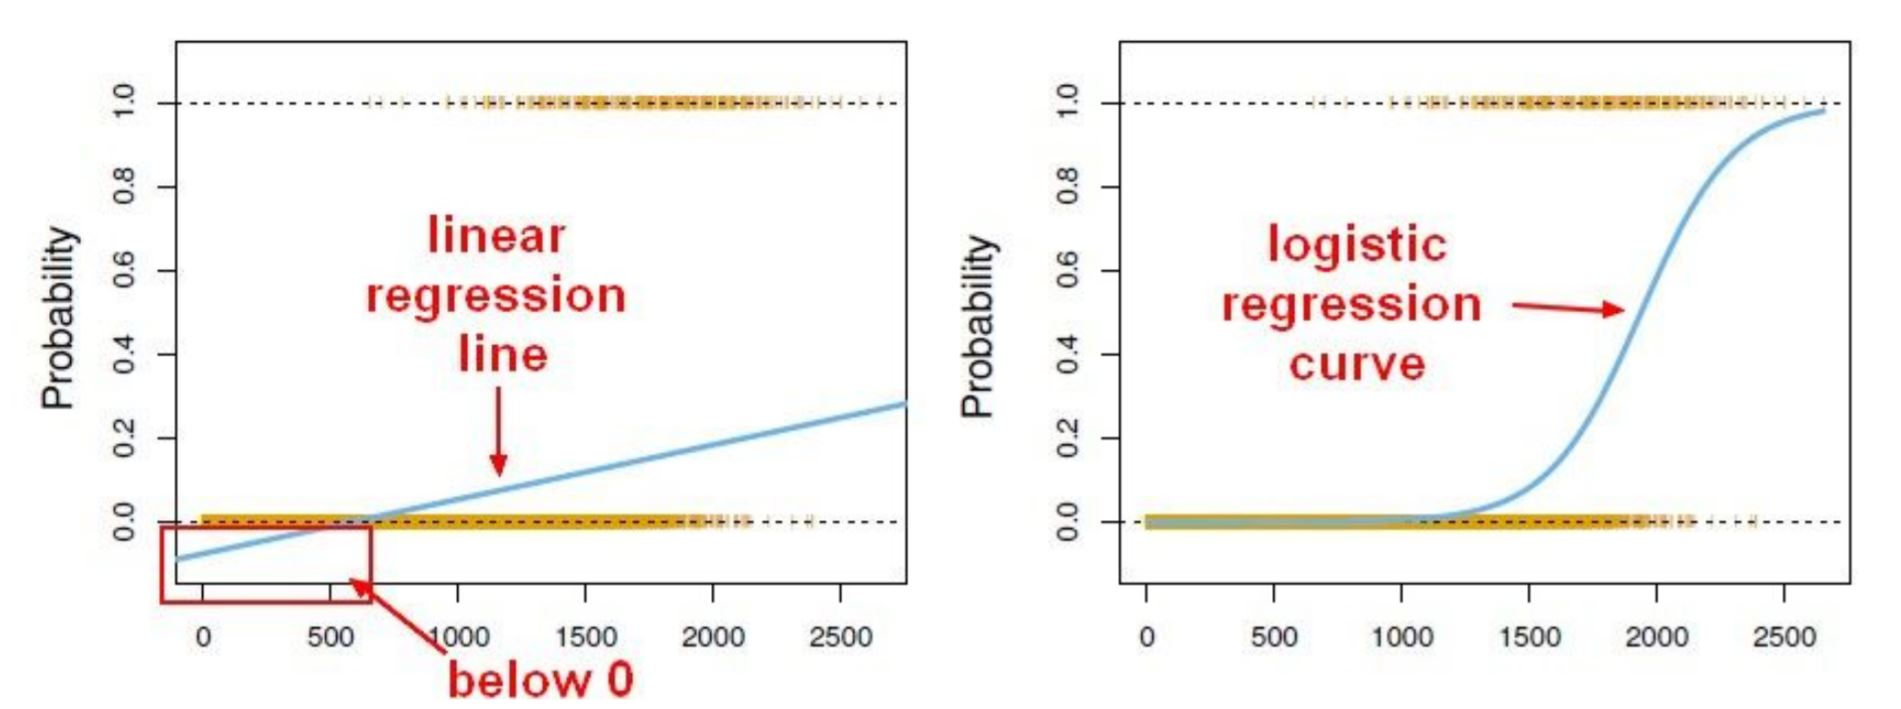
\includegraphics[width=0.9\textwidth]{pics/logistic_regression}
	\caption{Linear vs. Logistic regression} 
	\label{lin_log_regr}
\end{figure}
%         --------------------------------------

Sigmoid (aka Logistic) function takes in any value and outputs it between 0 and 1:
\[ \phi(z) = \frac{1}{1+e^{-z}}
\]
hence we can use Linear Regression solution $y=b_0+b_1 x$ and replace it\footnote{Note that an exponential function turns any score, even negative, into a positive one.} into $z$ - also see section \ref{multinominal} : 
%          --------   FIGURE: sigmoid  -----------
\begin{figure}[htbp] 
	\centering
	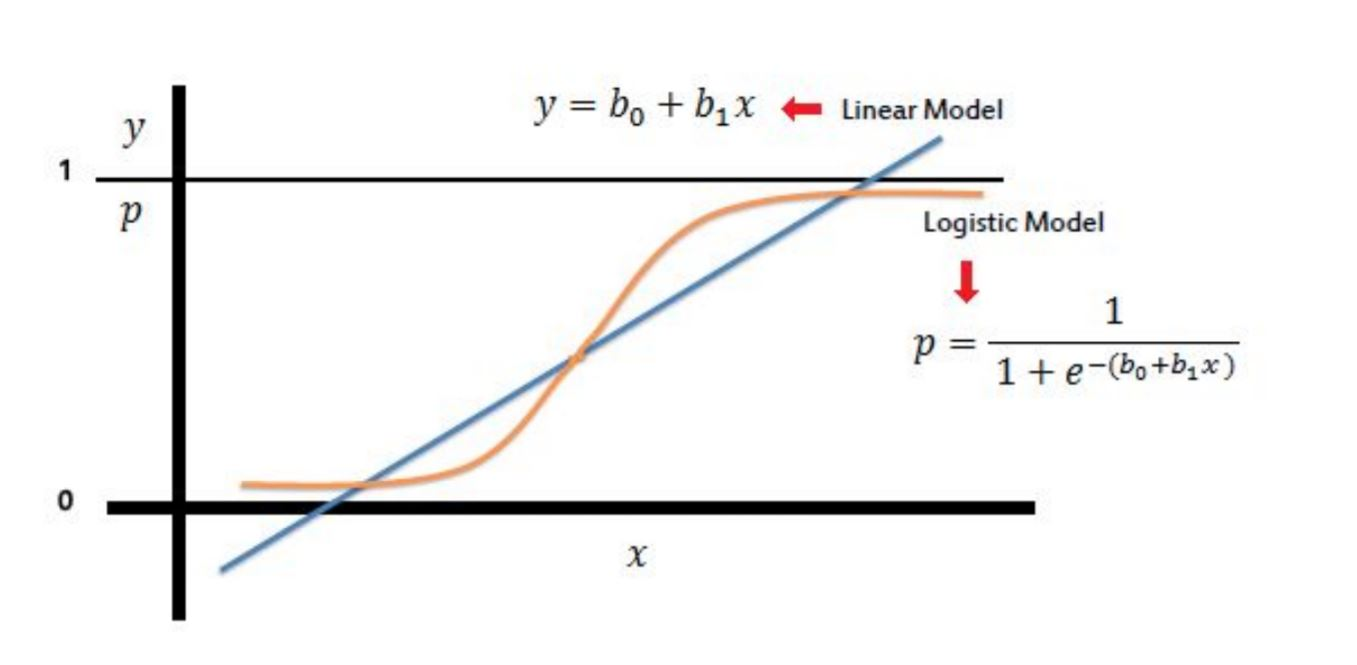
\includegraphics[width=0.7\textwidth]{pics/sigmoid}
	\caption{From linear to logistic}  
	\label{sigmoid}
\end{figure}
%         --------------------------------------

returning the \textbf{probability} (between 0 and 1) of belonging to a class: class 0 if prob below 0.5 and class 1 if above (see \ref{lin_log_regr}). 

Use \textbf{confusion matrix} to evaluate the model (e.g. disease vs. test) and true positive/true of the Logistic (or any classification model)
%          --------   FIGURE: confusion matrix  -----------
\begin{figure}[htbp] 
	\centering
	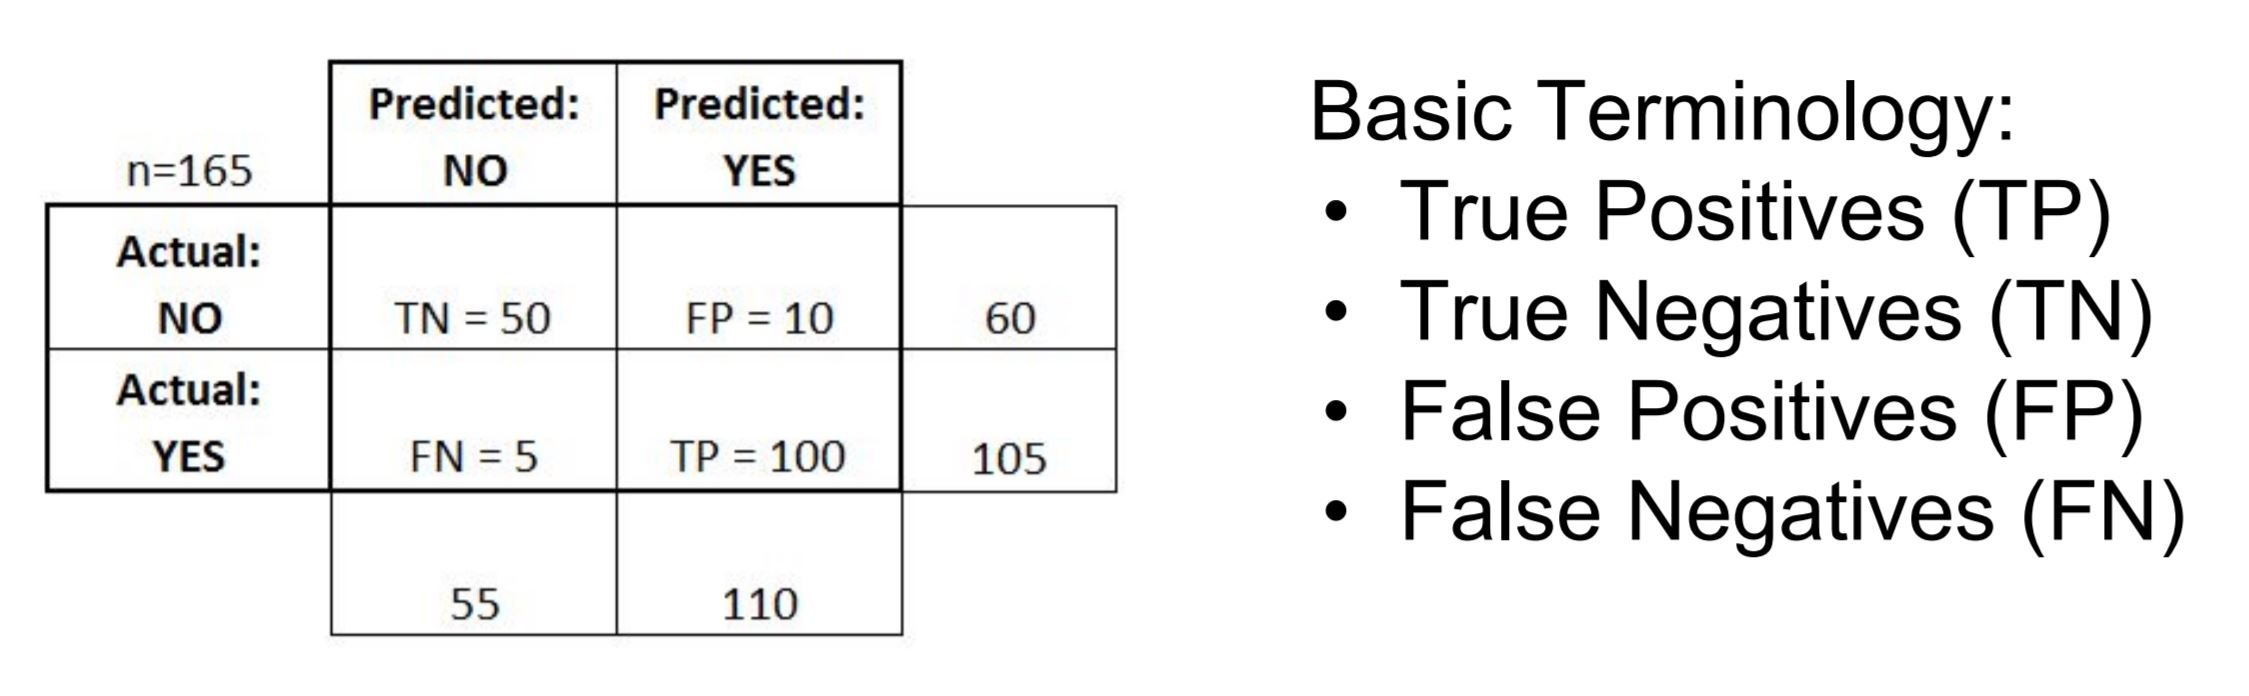
\includegraphics[width=0.7\textwidth]{pics/confusion_matrix}
	\caption{Confusion matrix}  
	%\label{XXXX}
\end{figure}
%         --------------------------------------

This is a \textit{short} list of rates that are often computed from a confusion matrix for a binary classifier:
\begin{itemize}
	\item \textbf{Accuracy}: (TP+TN)/tot = (100+50) / 165) = 0.91
	\item Error rate: (FP+FN)/tot = 1 - Accuracy
	\item \textbf{Recall} (or Sensitivity or True Positive Rate): TP/(\textit{actual} positive) = 100 / 105 = 0.95 (where 'actual positive' = TP + FN)
	\item Specificity: TN/(actual negative) = 50 / 60
	\item \textbf{Precision} TP/(\textit{predicted} positive) = 100 / 110 = 0.91 (where 'predicted positive' = TP + FP)
\end{itemize}
Use Precision and Recall rather than Accuracy rate (see 'accuracy paradox\footnote{For classification problems that are skewed in their classification distributions - e.g. if we had a 100 text messages and only 2 were spam and the rest 98 were not - accuracy by itself is not a very good metric. We could classify 90 messages as not spam (including the 2 that were actually spam, hence they would be false negatives) and 10 as spam (all 10 false positives) and still get a reasonably good accuracy score of 90\%. For such cases, precision and recall come in very handy. These two metrics can be combined to get the F1 score, which is weighted (harmonic) average of the precision and recall $F1\_score = 2 * \frac{prec * rec}{prec + rec}$} in wikipedia).

\begin{itemize}
	\item \textbf{Type I error} = False positive. \\ E.g. In a spam model, clearly worse to have a false positive (i.e. sending to the spam folder a non-spam email) than just the inconvenience of deleting a spam email that makes it to your inbox (false negative). Hence, we want to max \textbf{Precision} (up to 1. - how many spam emails correctly identified out of all \textit{predicted} spam ones);
	\item \textbf{Type II error} = False negative \\ E.g. In a medical context, a false negative (sick people sent back home because diagnosed as healthy) is clearly worse than false positives (healthy individuals that have to do more tests). Hence we want to maximise \textbf{Recall} (how many diagnosed sick out of all \textit{actual} sick people, e.g. precision 80\% but recall 95\%.).
\end{itemize}

Other \textit{evalutation metrics} are $F_{beta}$ (which is a generalisation of  $F1\_score$, see fig. \ref{F_beta_boundaries}) and Receiver Operating Characteristic ('ROC') curve (where the points are True Positive and True Negative Rate splitting, between (0, 0) and (1, 1))
%          --------   FIGURE: F_beta_boundaries  -----------
\begin{figure}[htbp] 
	\centering
	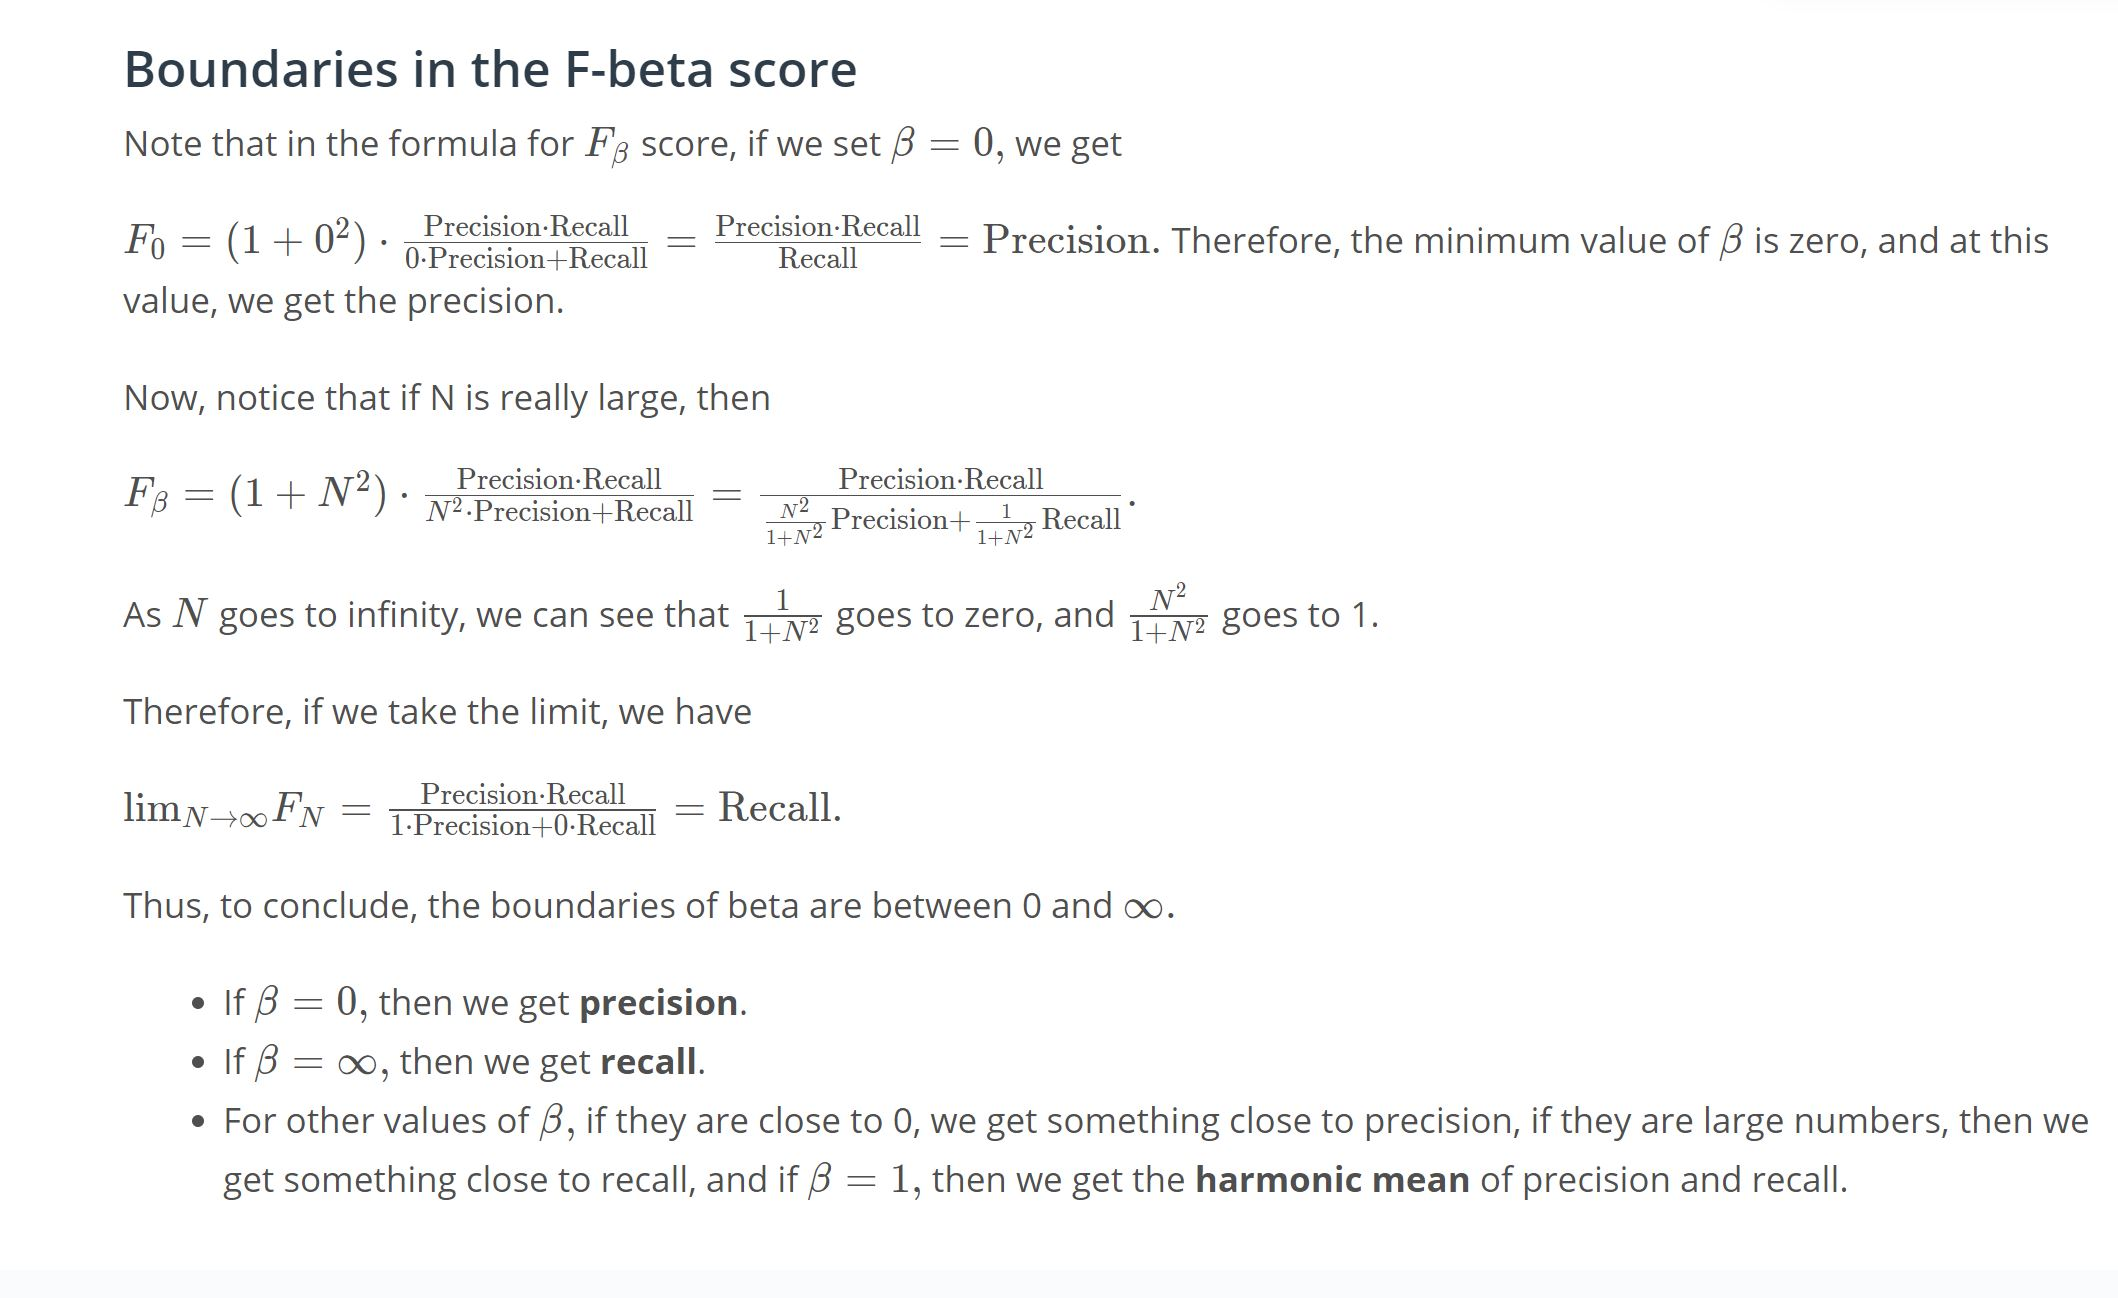
\includegraphics[width=0.85\textwidth]{pics/F_beta_boundaries}
	\caption{F beta}  
	\label{F_beta_boundaries}
\end{figure}
%         --------------------------------------

Learning curves plots the prediction accuracy/error vs. the training set size (ie: how better does the model get at predicting the target as you the increase number of instances used to train it)

And now the code:
\begin{lstlisting}
train = pd.read_csv('titanic_train.csv')  # load data

# heatmap to visualise missing data
sns.heatmap(train.isnull(),yticklabels=False,cbar=False,cmap='viridis')

# 1. visualise data
sns.set_style('whitegrid')
sns.countplot(x='Survived',hue='Sex',data=train,palette='RdBu_r')
sns.countplot(x='Survived',hue='Pclass',data=train,palette='rainbow')
sns.distplot(train['Age'].dropna(),kde=False,bins=30) # or
train['Age'].hist(bins=30)  # NB: no .dropna() needed

# 2. clean data (wealthier passengers -> older)
plt.figure(figsize=(12, 7))
sns.boxplot(x='Pclass',y='Age',data=train,palette='winter')

def impute_age(cols):
	Age = cols[0]
	Pclass = cols[1]
	if pd.isnull(Age):  # data missing
		if Pclass == 1:
			return 37
		elif Pclass == 2:
			return 29
		else:
			return 24
	else:
		return Age

 # apply fnct - NB: axis=1
train['Age'] = train[['Age','Pclass']].apply(impute_age,axis=1)

 # drop a useless col and na rows
train.drop('Cabin',axis=1,inplace=True)
train.dropna(inplace=True)

# 3. convert categorical vars into dummy variables 
# dummies for a series, then concat axis=1
sex = pd.get_dummies(train['Sex'],drop_first=True)
# or, alternatively, train['Sex'] = train.Sex.map({male:1, female:0})
embark = pd.get_dummies(train['Embarked'],drop_first=True)
 # remove unnecessary cols
train.drop(['Sex','Embarked','Name','Ticket'],axis=1,inplace=True)
 # get new cols in (NB: axis=1)
train = pd.concat([train,sex,embark],axis=1)

# alternative: apply dummies to the col & rtrn all
final_data = pd.get_dummies(df_loans,columns=["colum_name"],drop_first=True)

# 4. build model
 # train
X_train, X_test, y_train, y_test = 
	 train_test_split(train.drop('Survived',axis=1), 
		train['Survived'], test_size=0.30, random_state=101)
 # build 		
from sklearn.linear_model import LogisticRegression
logmodel = LogisticRegression()
logmodel.fit(X_train,y_train)

predictions = logmodel.predict(X_test)

 # evaluate
from sklearn.metrics import classification_report
print(classification_report(y_test,predictions))
\end{lstlisting}

%          --------   FIGURE: ROC Curve -----------
\begin{figure}[htbp] 
	\centering
	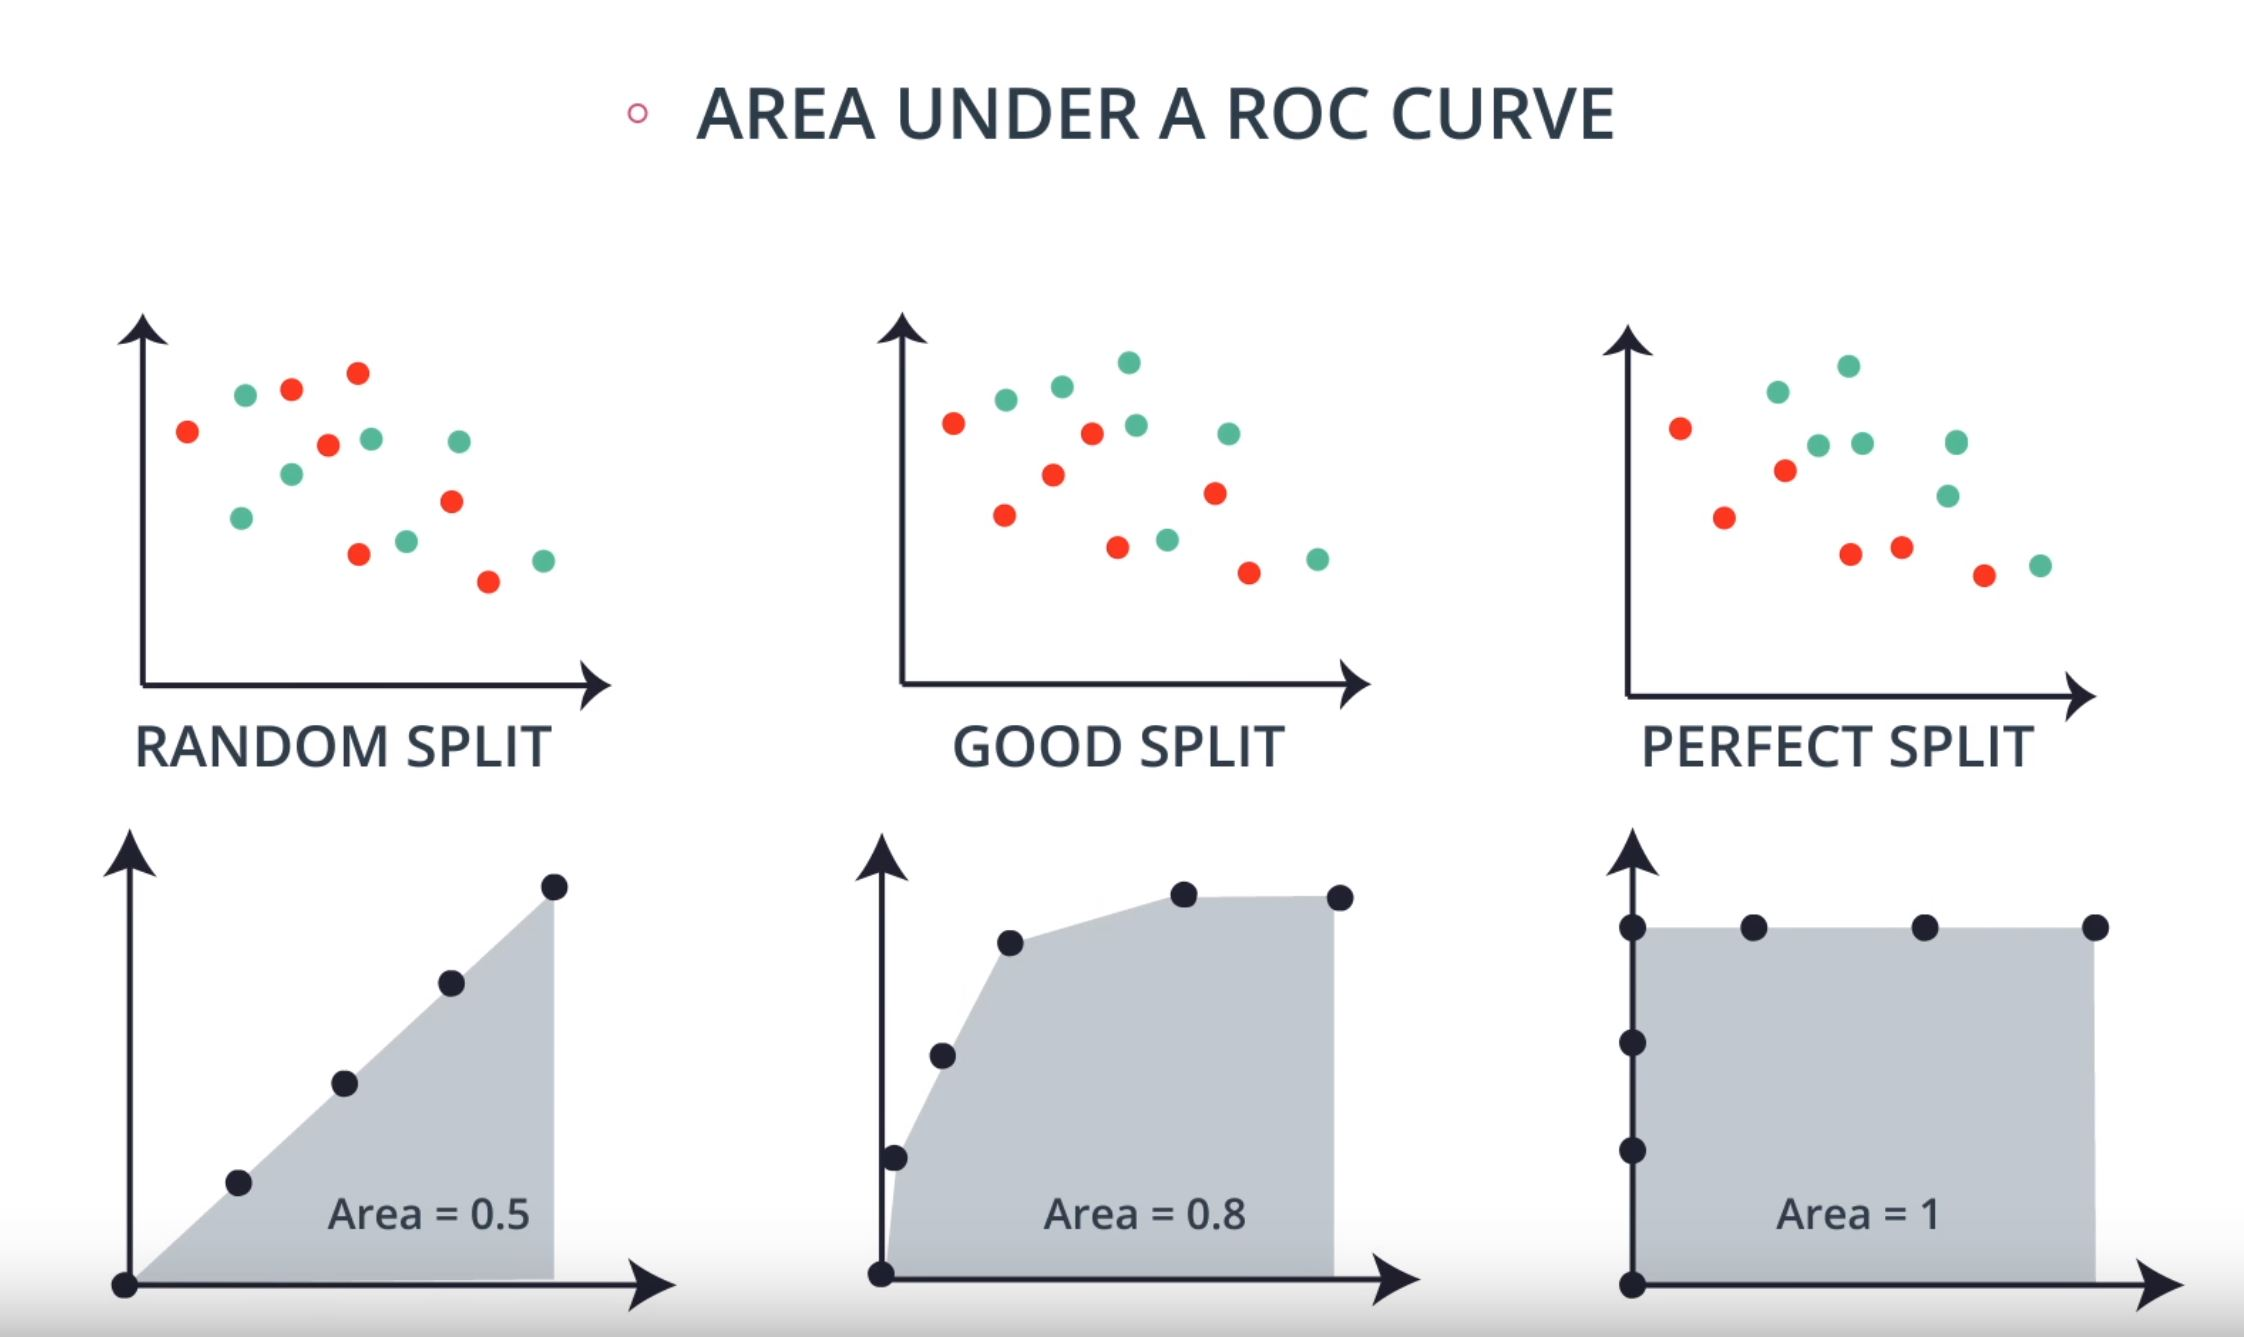
\includegraphics[width=0.6\textwidth]{pics/ROC_curve}
	\caption{ROC curve}  
	\label{ROC_curve}
\end{figure}
%         --------------------------------------


%%%%%%%%
To recap, the \textbf{evaluation metrics} are:
\begin{itemize}
	\item \underline{regression}: mean absolute error (but not differentiable), mean square error, R2.
	\item \underline{classification}: accuracy (but note for skew distributions), precision and recall, $F1\_score$ and its generalisation, ROC.
\end{itemize}


%%%%%%%%%%%%%%%%%%%%%%%%%%%%%%%%%%%%%%%%%%%%%%%%%%%%%%
\subsection{Bayes Learning} \label{Bayes} 

\subsubsection{Naive Bayes}
The probabilistic model of naive Bayes classifiers is based on Bayes' theorem, and the adjective \textit{naive} comes from the fact that the algorithm considers the features (or attributes) that it is using to make the predictions to be mutually \textit{independent}, which may not always be the case (e.g. a naive Bayes spam filter considers the frequency, but not the order of the words). In practice, the independence assumption is often violated, but naive Bayes classifiers still tend to perform very well under this unrealistic assumption - especially for small sample sizes.

One of the major advantages that Naive Bayes has over other classification algorithms is its ability to handle an extremely large number of features. For example, in a spam detector algorithm each word is treated as a feature and there are thousands of different words. Also, it performs well even with the presence of irrelevant features and is relatively unaffected by them. The other major advantage it has is its relative simplicity. Naive Bayes' works well right out of the box and tuning it's parameters is rarely ever necessary, except usually in cases where the distribution of the data is known. It rarely ever overfits the data. Another important advantage is that its model training and prediction times are very fast for the amount of data it can handle. 

Example, if $h = Cancer$ and $D (data) = \text{positive test}$:
\[ \underbrace{P(Cancer|Pos)}_{\text{a posteriori}} = \frac{ P(Pos|Cancer) \; \overbrace{P(Cancer)}^{\text{a priori}} }{P(Pos)} 
\]
%          --------   Bayes:   -----------
\begin{figure}[htbp] 
	\centering
	\includegraphics[width=0.7\textwidth]{pics/bayesian_learning}
	\caption{Bayes learning} 
	\label{bayesian_learning}
\end{figure}
%         --------------------------------------


\begin{lstlisting}
from sklearn.naive_bayes import MultinomialNB, GaussianNB
naive_bayes = MultinomialNB()  # GaussianNB
naive_bayes.fit(training_data, y_train)
predictions = naive_bayes.predict(testing_data)
\end{lstlisting}


Note that the final expression is the OLS in fig. \ref{bayesian_learning2} or perceptron: if Hp is linear and errors are i.i.d and Gaussians, we recover regression (e.g. $x_i$ are heights and $d_i$ the weights of people)

%          --------   Bayesain Learning 2  -----------
\begin{figure}[htbp] 
	\centering
	\includegraphics[width=0.7\textwidth]{pics/bayesian_learning_2}
	\caption{Bayes learning 2} 
	\label{bayesian_learning2}
\end{figure}
%         --------------------------------------

Note that $lg$ in fig. \ref{bayesian_learning3} is the $log$ in base $2$ (number of bits). This is showing the link to entropy (error/wrong labels and size of hp): you want to find the simplest hypothesis that minimise the errors (usually the two terms are a trade-off: complicated hypothesis tend to reduce errors and vice-versa). This is called the "minimum description lenght". This justifies, somehow, the Occam's razor.
%          --------   Bayesain Learning 3  -----------
\begin{figure}[htbp] 
	\centering
	\includegraphics[width=0.7\textwidth]{pics/bayesian_learning_3}
	\caption{Minimum description lenght} 
	\label{bayesian_learning3}
\end{figure}
%         --------------------------------------

Once we find $P(h|D)$ we really need to get a classification: see formula in fig. \ref{bayesian_learning4} 
%          --------   Bayesain Learning 4  -----------
\begin{figure}[htbp] 
	\centering
	\includegraphics[width=0.7\textwidth]{pics/bayesian_learning_4}
	\caption{Bayes classification} 
	\label{bayesian_learning4}
\end{figure}
%         --------------------------------------

\subsubsection{Belief Networks}
Belief Networks (also called Bayes Nets or Bayesian Networks or Graphical Models) represent - graphically (via nodes and branches) - conditionally probabilities on events - and any joint probability comes from multiplying such conditional ones. If not independent, then it grows exponentially since you get more branches going into same event/node. Dependence does not mean causality (obviously). \textit{Topological} order (for sampling the joint distribution): it must be acyclic (you need to go from parent(s) to children).

%          --------   Bayesain Learning 4  -----------
\begin{figure}[htbp] 
	\centering
	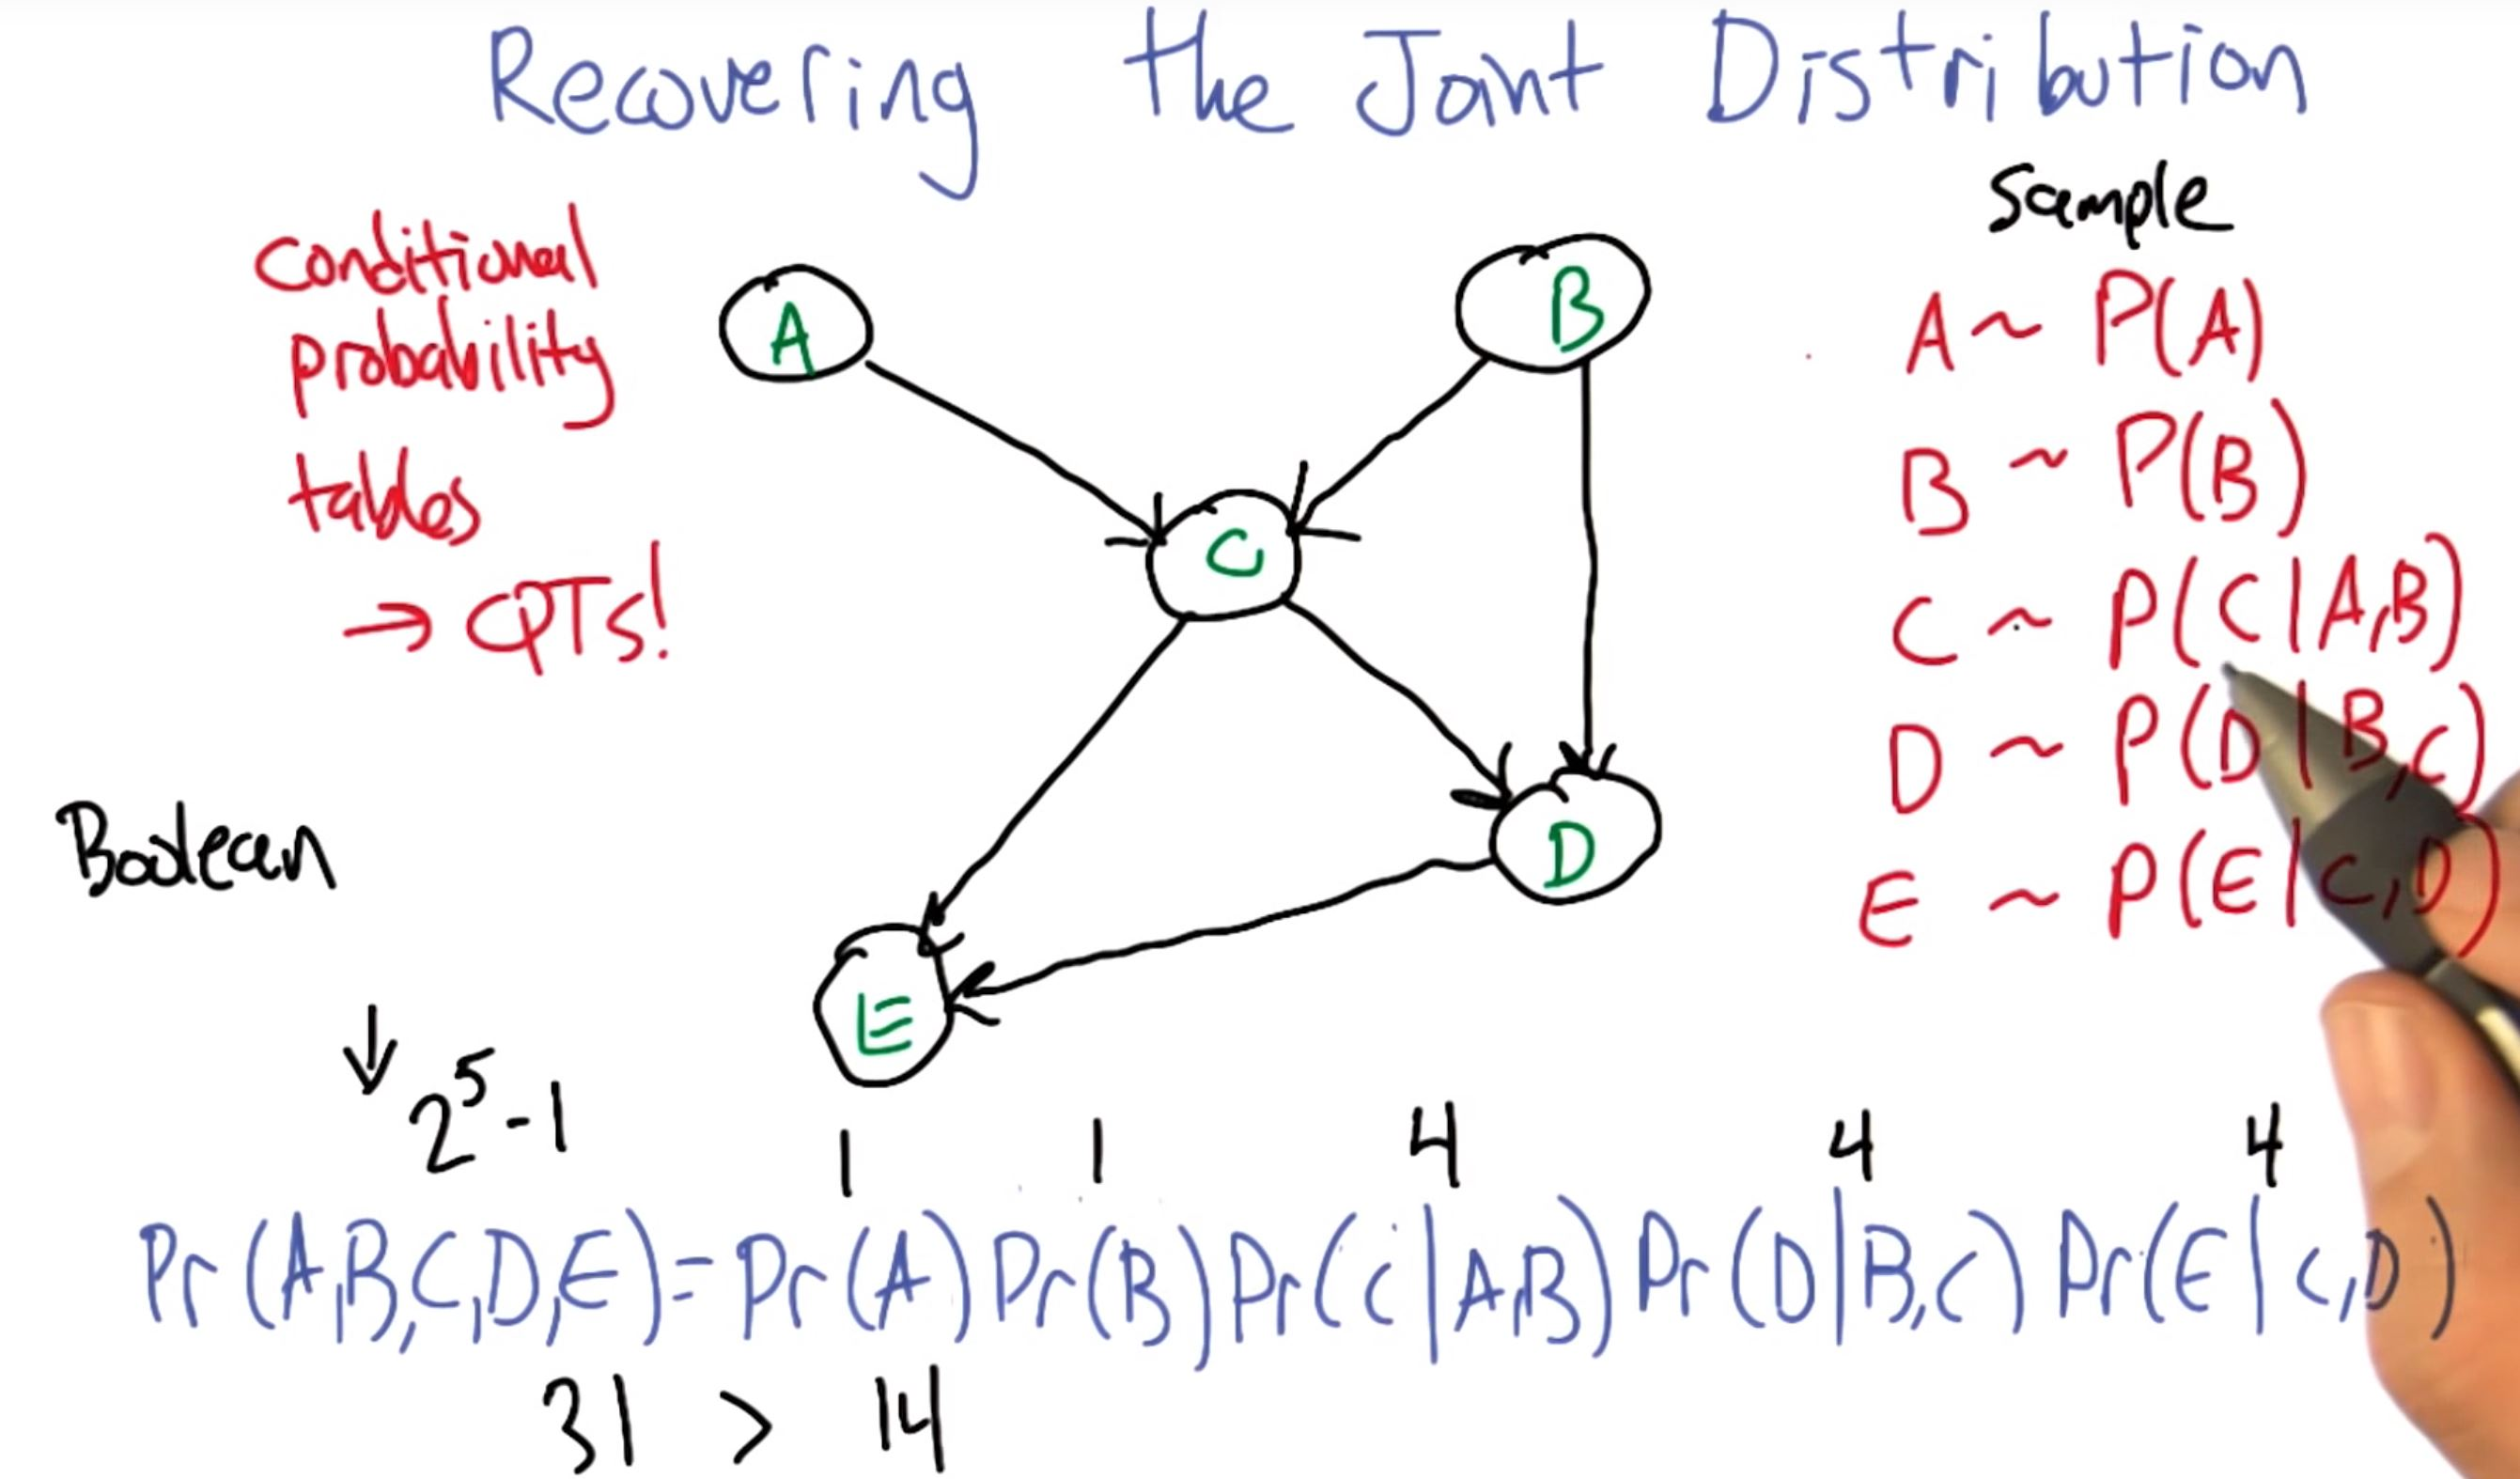
\includegraphics[width=0.9\textwidth]{pics/belief_network1}
	\caption{Sampling} 
	\label{belief_network1}
\end{figure}
%         --------------------------------------
Belief networks can be useful for approximate inference (simulate/generate some samples to infer 'reverse' conditional probability - easier to solve and faster), visualitation (get a fee), simulation of complex process. 

%          --------   Bayesain Learning 5  -----------
\begin{figure}[htbp] 
	\centering
	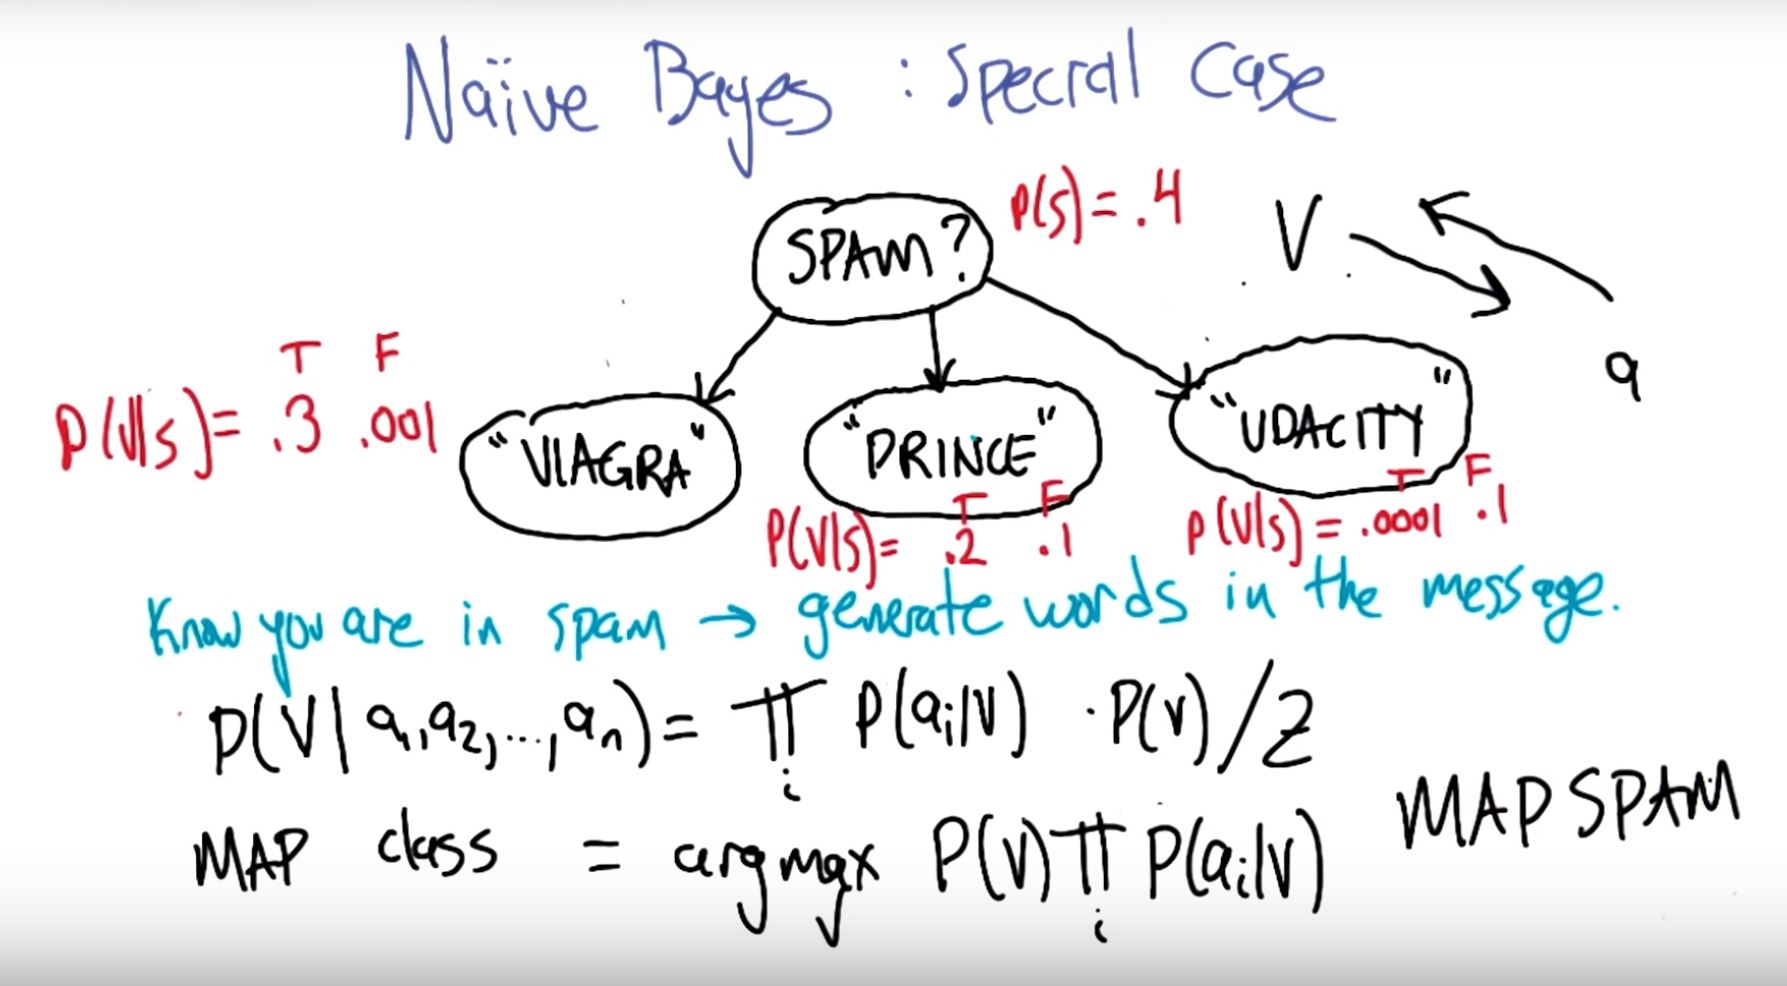
\includegraphics[width=0.9\textwidth]{pics/Bayesian_special_case}
	\caption{Bayes SPAM (Bayes link to classification)} 
	\label{Bayesian_special_case}
\end{figure}
%         --------------------------------------

Why Naive Bayes is cool:
\begin{itemize}
	\item inference (in any direction) is cheap - linear rather than exponential (just using Bayes formula);
	\item few parameters;
	\item estimate parameters with labelled data: $Pr(attr_i | Class) = \frac{\# \, attr_{i,C}}{\# \, C}$ (one unseen attribute may spoil the whole classification, hence 'smooth' applied or the inductive bias);
	\item connect inference and classification;
	\item empirically succesful. Even if the model does not model interrelationships beetween atributes, it is still able to preserve the order (which in classification is what we care about).	 
\end{itemize}

\subsubsection{Bag of Words}
 Bag of Words(BoW) is a concept used to specify the problems that have a collection of text data that needs to be worked with. The basic idea of BoW is to take a piece of text and count the frequency of the words in that text. It is important to note that the BoW concept treats each word individually and the order in which the words occur does not matter (it is a 'naive' Bayes, indeed).

From scratch:
\begin{lstlisting}
from import CountVectorize
# TO BE COMPLETED
\end{lstlisting}

From scratch:
\begin{lstlisting}
#
#	INSERT 
#
\end{lstlisting}

%%%%%%%%%%%%%%%%%%%%%%%%%%%%%%%%%%%%%%%%%%%%%%%%%%%%%%
\subsection{K Nearest Neighbours} \label{K_Nearest_Neighbours} 
KNN is a (non parametric) classification (or regression, see below) algorithm based on a simple principle, first one stores all the data (training) and then follows the steps below for the prediction:
\begin{itemize}
	\item calculate distance from $q$ to all points $x_i$ in your data,
	\item sort the data by increasing distance from $q$ (or some other similarity: our domain knowledge),
	\item predict $q$ using majority label of the 'K' closest pointss.
\end{itemize}
Example: think about cost label of a house (e.g. expensive, medium, cheap) vs. some nearby houses we know the price/labels of - how many houses ('K') are to be considered in a neighbourhood? say e.g. 5, calculate the distances, rank and get closest 5 houses, predict our unknown-label house using the majority label of such 5 closest houses.  

The choice of K will clearly affect what class new point is assigned to (k=1 is very noisy, ...) as it does the choice of distance (e.g. Euclidean vs. L1-norm / Manhattan). Simple, but not good for large data sets and for categorical features.

Preference bias of KNN (our belief of what makes a good Hp):
\begin{itemize}
	\item locality (near points are \underline{similar}: \textbf{distance}, e.g. Euclidean vs. L1),
	\item smoothness (\textbf{averaging}),
	\item all features matter \underline{equally} (think of using KNN regression on a function that was actually $y=x_1^2 + x_2$, clearly $x_1$ more important and KNN will not be that good).
\end{itemize}

Why standardise the variables: the KNN classifier predicts the class of a given test observation by identifying the observations that are nearest to it, therefore the scale of the variables matters (large scale variables will have a much larger effect on the distance and hence on the KNN classifier).
\begin{lstlisting}
# 1. read data
df = pd.read_csv("Classified Data",index_col=0)

# 2. standardise variables (import, fit and transform)
from sklearn.preprocessing import StandardScaler
scaler = StandardScaler() # initialise
scaler.fit(df.drop('TARGET CLASS',axis=1)) # targ class = 0 or 1
scaled_features = scaler.transform(df.drop('TARGET CLASS',axis=1))
# scaled_feature is an array now, so we re-create df
# note: scaled_fatures will also work in train or KNN algo
df_feat = pd.DataFrame(scaled_features,columns=df.columns[:-1])

# 3. build model
  # train test split
from sklearn.model_selection import train_test_split
X_train, X_test, y_train, y_test = 
	train_test_split(scaled_features,df['TARGET CLASS'],
		test_size=0.30)

 # using KNN (starting with K =1)
from sklearn.neighbors import KNeighborsClassifier
knn = KNeighborsClassifier(n_neighbors=1)  # K = 1
knn.fit(X_train,y_train)
pred = knn.predict(X_test)
 
 # evaluate
from sklearn.metrics import classification_report,confusion_matrix
print(confusion_matrix(y_test,pred))
print(classification_report(y_test,pred))
# from sklearn.metrics import accuracy_score, precision_score, recall_score, f1_score
# print(accuracy_score(y_test, pred))

 # choose right K value
error_rate = []
for i in range(1,40):  # will take some time
	knn = KNeighborsClassifier(n_neighbors=i)
	knn.fit(X_train,y_train)
	pred_ = knn.predict(X_test)
	error_rate.append(np.mean(pred_ != y_test))

plt.figure(figsize=(10,6))
plt.plot(range(1,40),error_rate,color='blue', ls='dashed', 
  marker='o', markerfacecolor='red', markersize=10)
plt.title('Error Rate vs. K Value')
plt.xlabel('K')
plt.ylabel('Error Rate')
\end{lstlisting}
You see that after, say, K$>$20 the error rate just tends to hover around, say, 0.06-0.05. Get confusion matrix and classification report with say K=20 and compare vs. those of K=1.

Instance-based learning in general
Advantage: (i) it does not forget data (e.g. in regression, we fit the model to the training data but we don't use it anymore), (ii) fast and (iii) simple. But: (i) no generalisation and (ii) overfit.

\textit{Curse of dimensionality}: as the number of features or dimensions grows, the amount of data we need to generalise accurately grows \underline{exponentially}. E.g. 10 points in 1 dim, become 100 in 2-dim and 1000 in 3-dim... This is an issue for KNN only.

%%%%%%%%%%%%%%%%%%%%%%%%%%%%%%%%%%%%%%%%%%%%%%%%%%%%%%
\subsubsection{KNN regression}
Above we saw the KNN classifier, here we look at the KNN regression (i.e. y's are numbers rather than labels) - this is a non-parametric regression, we predict y as the \textit{mean} of y's rather the more frequent label (i.e. regression: mean of $y_i$ in NN vs. classification: vote/plurality/majority of the $y_i$).

LOOK AT MY NOTES

\subsubsection{Kernel regression}
Difference: here we weight the contribution of each $x_i$ we have based on how far away from $x$ at hand, whilst in KNN regression every $x$ is essentially equally-weighted. For example, we can replace the average with locally-weighted regression or even Neural Networks or other algorithms.

%%%%%%%%
To recap:
\begin{itemize}
	\item parametric: if problem is biased, meaning that you have an idea of the relationship in terms of functional form, then use a parametric model/approach (e.g. how far a cannon is going to shoot, given the angle);
	\item non-parametric: for un-biased problems, when you have no idea of the functional forms, then best to use a non-parametric approach (e.g. bees population as function of the food richness). More data-intensive since you have to store all data, but no need to guess the form of the solution.
\end{itemize}


In \textbf{eager} learners, e.g. Naive Bayes or regression, the computationally most expensive step is the model building (learning the model from a training dataset) whereas the classification of new instances is relatively fast (once model is learned).

\textbf{Lazy} learners, like KNN, instead memorise and re-evaluate the training dataset for predicting the class label of new instances. Here is the model building step that is relatively fast, whilst the actual prediction is typically slower due to the re-evaluation of the training data. Another disadvantage of lazy learners is that the training data has to be retained, which can also be expensive in terms of storage space.

Note that - assuming sorted data points - (i) in linear regression the learning runnig time is $n$ (filling matrix and inverting), whilst querying is constant (fast), (ii) instead for KNN is almost the reverse: learning speed is constant but query is $log(n)$. 

Every time a new instance is encountered, KNN would evaluate the k-nearest neighbours in order to decide upon a class label for the new instance, e.g., via the majority rule (i.e., the assignment of the class label that occurs most frequently amongst the k-nearest neighbors).

%%%%%%%%%%%%%%%%%%%%%%%%%%%%%%%%%%%%%%%%%%%%%%%%%%%%%%
\subsection{Decision Trees and Random Forests}
E.g. shall I enter this restaurant or not? possible instances/features: type of cuisine (Italian, French, ...), atmosphere (fancy, casual, ...), occupied, costs (discrete or number), hungry?, raining (would like to stop now), ... 

Representation: what is a decision tree vs. algorithm (latter is how you implement such representation).

Representation: a tree is made-up of
\begin{itemize}
	\item Nodes: defined by the value of a certain \textit{attribute}, using questions for further splits or arrival point; 
	\item Edges or branches: outcome of a split to the next node (represent \textit{values}, i.e. answers to the question in preceding node)
\end{itemize}
also nodes are of two kinds:
\begin{itemize}
	\item Decision nodes (that topmost called root node): node that performs splits (usually drawn as a circle, it has two or more branches);
	\item Leaf notes: \textit{terminal} nodes that represent the outcome(s) (usually drawn as a boxe or just the end-result), they've got just one branch to a decision node or no branches (for the final ones).
\end{itemize}

The goal is to narrowing possibilities in getting the right class. Algorithm: pick best attributes and ask questions (e.g. best: halving possibilities), follow answer path and repeat (questions get more and more specific) until got an answer. 

\textbf{Entropy} (that measures the homogeneity of a data set, from zero to the $log_2$ of different classes\footnote{E.g. for two classes: if all samples belong to one class then entropy is zero (no uncertainty), if data equally split between the two classes ($p_1 = p_2 = 0.5$) then entropy is 1 (the max for two classes). You can think of it as a parable with max of 1 at p=0.5 and minima of zero when p is either 0 or 1,}) and Information Gain (how well an attribute splits the data into groups based on classification: it measures the reduction in entropy that results from partitioning the data on an attribute) are the Mathematical Methods of choosing the best split (ref Ch 8 of Gareth et al):
\[ Gain(S, A) = Entropy(S) - \sum_v \frac{|S_v|}{|S|} Entropy(S_v)
\]
where $S$ is the collection of training examples, $A$ is the attribute, $v$ is a particular class. And, finally, Entropy is $-\sum_v p(v) \,log_2[p(v)]$ (a measure of randomness or information). Recall that p(v) is the fraction of examples in class v. The above equation can be seen as a difference between entropy before and after the split - hence the higher the Information Gain, the lower the entropy after the split.

In short, constructing a decision tree is all about finding attribute that returns the highest Information Gain (i.e., the most homogeneous branches). Note that in sklearn DecisionTreeClassifier the default criterion is the Gini index ('gini'), rather than the information gain ('entropy').  

\textit{Expressiveness} (i.e. space of our hypothesis): n-or linear tree vs. n-xor\footnote{Difference: 'xor' is only true when either $x$ or $y$ are true, but not both (as instead for 'or'), i.e. is exclusive vs. inclusive.} (e.g. odd parity: true if odd no. of T) tree nodes are $o(2^n)$, very hard (being exponential fnct). 
Suppose we have $n$ boolean attributes and output is boolean, how many trees (or rows in a truth table) are needed? rows are $2^n$ and trees are even more: $2^{2^n}$ (which is not $4^n$ and after just n=6 already explodes). 

Example of algorithm (implementation): ID3 - a top-down, greedy search through the space of possible branches with no backtracking. ID3 uses Entropy and Information Gain to construct a decision tree:
\begin{itemize}
	\item Calculate entropy of the target.
	\item The dataset is then split on the different attributes. The entropy for each branch is calculated. Then it is added proportionally, to get total entropy for the split. The resulting entropy is subtracted from the entropy before the split, the result is the Information Gain or decrease in entropy. 
	\item choose the attribute with the largest information gain as decision node; repeat for each new branch (if the entropy of the branch is zero 0 all yes or all no -  is a leaf node, continuous untill all leaf nodes, i.e. all classified.)
\end{itemize}


ID3 biases. Restriction bias (hypothesis: considering only decision trees, not an infinite number but a well defined set) and preference bias (what we prefer from the hypothesis set vs. another). Inductive bias $->$ algo preferences: good splits at top, correct over incorret, shorter tres.

Other considerations for decision trees.
\begin{itemize}
	\item continuous attributes? what about for example 'age', we can use a range (e.g. a node with $20 \le age<30$ and since it is a continuous attribute we may ask again another question on it e.g. $age<20$).
	\item when do we stop? when everything correctly classified, no more (discrete) attributes, no overfitting (noise always inside data: use cross-validation or expand the tree until error does not drop much or 'pruning', which is collapsing the leaves if error small enough).
	\item regression: how to adapt a tree to continuous outputs. You need a different splitting criterion than information gain, e.g. variance, average of linear output.
\end{itemize}


A tree separates the space (decision boundaries), see \ref{tree_linear_separator}: two questions separates the space with two lines.
%          --------   FIGURE: tree_linear_separator  -----------
\begin{figure}[htbp] 
	\centering
	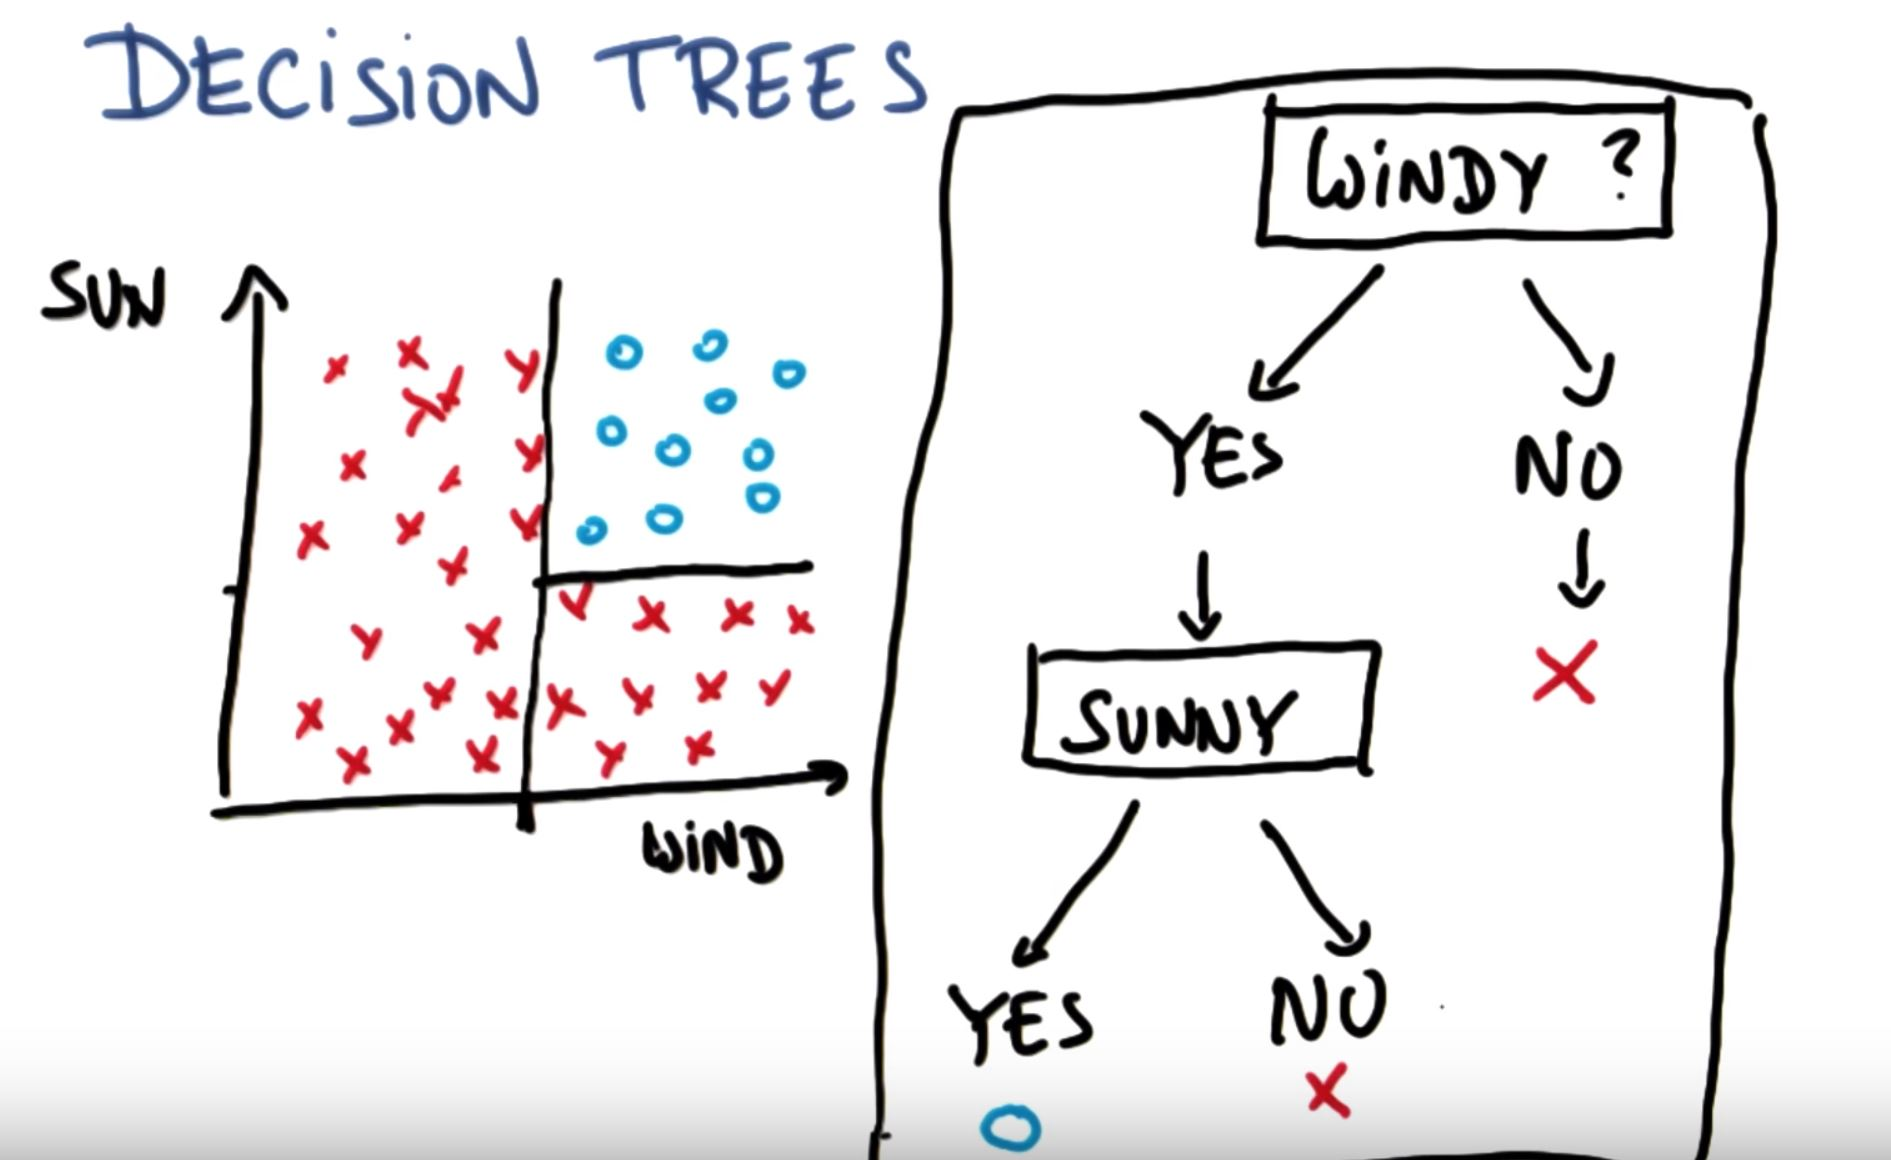
\includegraphics[width=0.6\textwidth]{pics/tree_linear_separator}
	\caption{Tree separator} 
	\label{tree_linear_separator}
\end{figure}
%         --------------------------------------


To improve performance, we can use many trees with a random sample of features chosen as the split.
\begin{itemize}
	\item  A new random sample of features is chosen for \textit{every single tree at every single split}.
	\item For classification, m (\# random features) is typically chosen to be the square root of p (\# total features).
\end{itemize}

Random Forests vs. Trees \\
Suppose there is \textit{one very strong feature} in the data set. When using “bagged” trees, most of the trees will use that feature as the top split, resulting in an ensemble of similar trees that are \textit{highly correlated}. Averaging highly correlated quantities does not significantly reduce variance. By randomly leaving out candidate features from each split, \textbf{Random Forests "decorrelates" the tree}s, such that the averaging process can reduce the variance of the resulting model.

\begin{lstlisting}
# 1. read data
df = pd.read_csv('kyphosis.csv')

# 2. visualise 
sns.pairplot(df,hue='Kyphosis',palette='Set1')

# 3. Decision Tree & Random Forest
 # train
from sklearn.model_selection import train_test_split
X_train, X_test, y_train, y_test = 
  train_test_split(df.drop('Kyphosis',axis=1),
   df['Kyphosis'], test_size=0.30)
  
  # build Decision Tree
from sklearn.tree import DecisionTreeClassifier
dtree = DecisionTreeClassifier()
dtree.fit(X_train,y_train)
predictions = dtree.predict(X_test)

 # build Random Forest (NB: .tree vs. .ensemble)
from sklearn.ensemble import RandomForestClassifier
rfc = RandomForestClassifier(n_estimators=100)
rfc.fit(X_train, y_train)
rfc_pred = rfc.predict(X_test)

 # evaluate
from sklearn.metrics import classification_report,confusion_matrix
print(confusion_matrix(y_test,predictions)) # for tree
print(confusion_matrix(y_test,rfc_pred))  # for rdm forest
# and same for classification_report
\end{lstlisting}

To reduce potential overfit, I can increase the min\_samples\_split (one param in DecisionTreeClassifier) from default of 2 (won't split samples lower than 2) to something bigger, e.g. 50.

%%%%%%%%%%%%%%%%%%%%%%%%%%%%%%%%%%%%%%%%%%%%%%%%%%%%%%
\subsection{Perceptrons} \label{perceptrons}

Cartoonish view of human neurons.

Perceptron (see fig. \ref{perceptron} for a graphic definition) always returns half-plane (e.g. immagine 2 inputs $X$ with equal weights $1/2$ and a threshold of $3/4$, then the perceptron divides the plan in two by the line passing for (0,3/2) and (3/2,0): 1 above and zero below) - i.e. linear threshold units.

If the 'net-input' - which is a linear combinations of weights and inputs,  $w^T x$, also called 'activation' - is above a threshold $\theta$ then the input belongs to one class, otherwise to the other (there are only two classes, a binary problem - NB: decision is a 'step function'). One can brings $\theta$ on the left of the equation to simplify the problem ($w_0 = \theta$, usually called the 'bias unit' - i.e. the new net-input is then compared to zero). In other words, the net input - $w^T x$ - is squashed into a binary output by the decision function, which is used to discriminate between two \textit{linearly-separable} classes.
%          --------   FIGURE: percepton  -----------
\begin{figure}[htbp] 
	\centering
	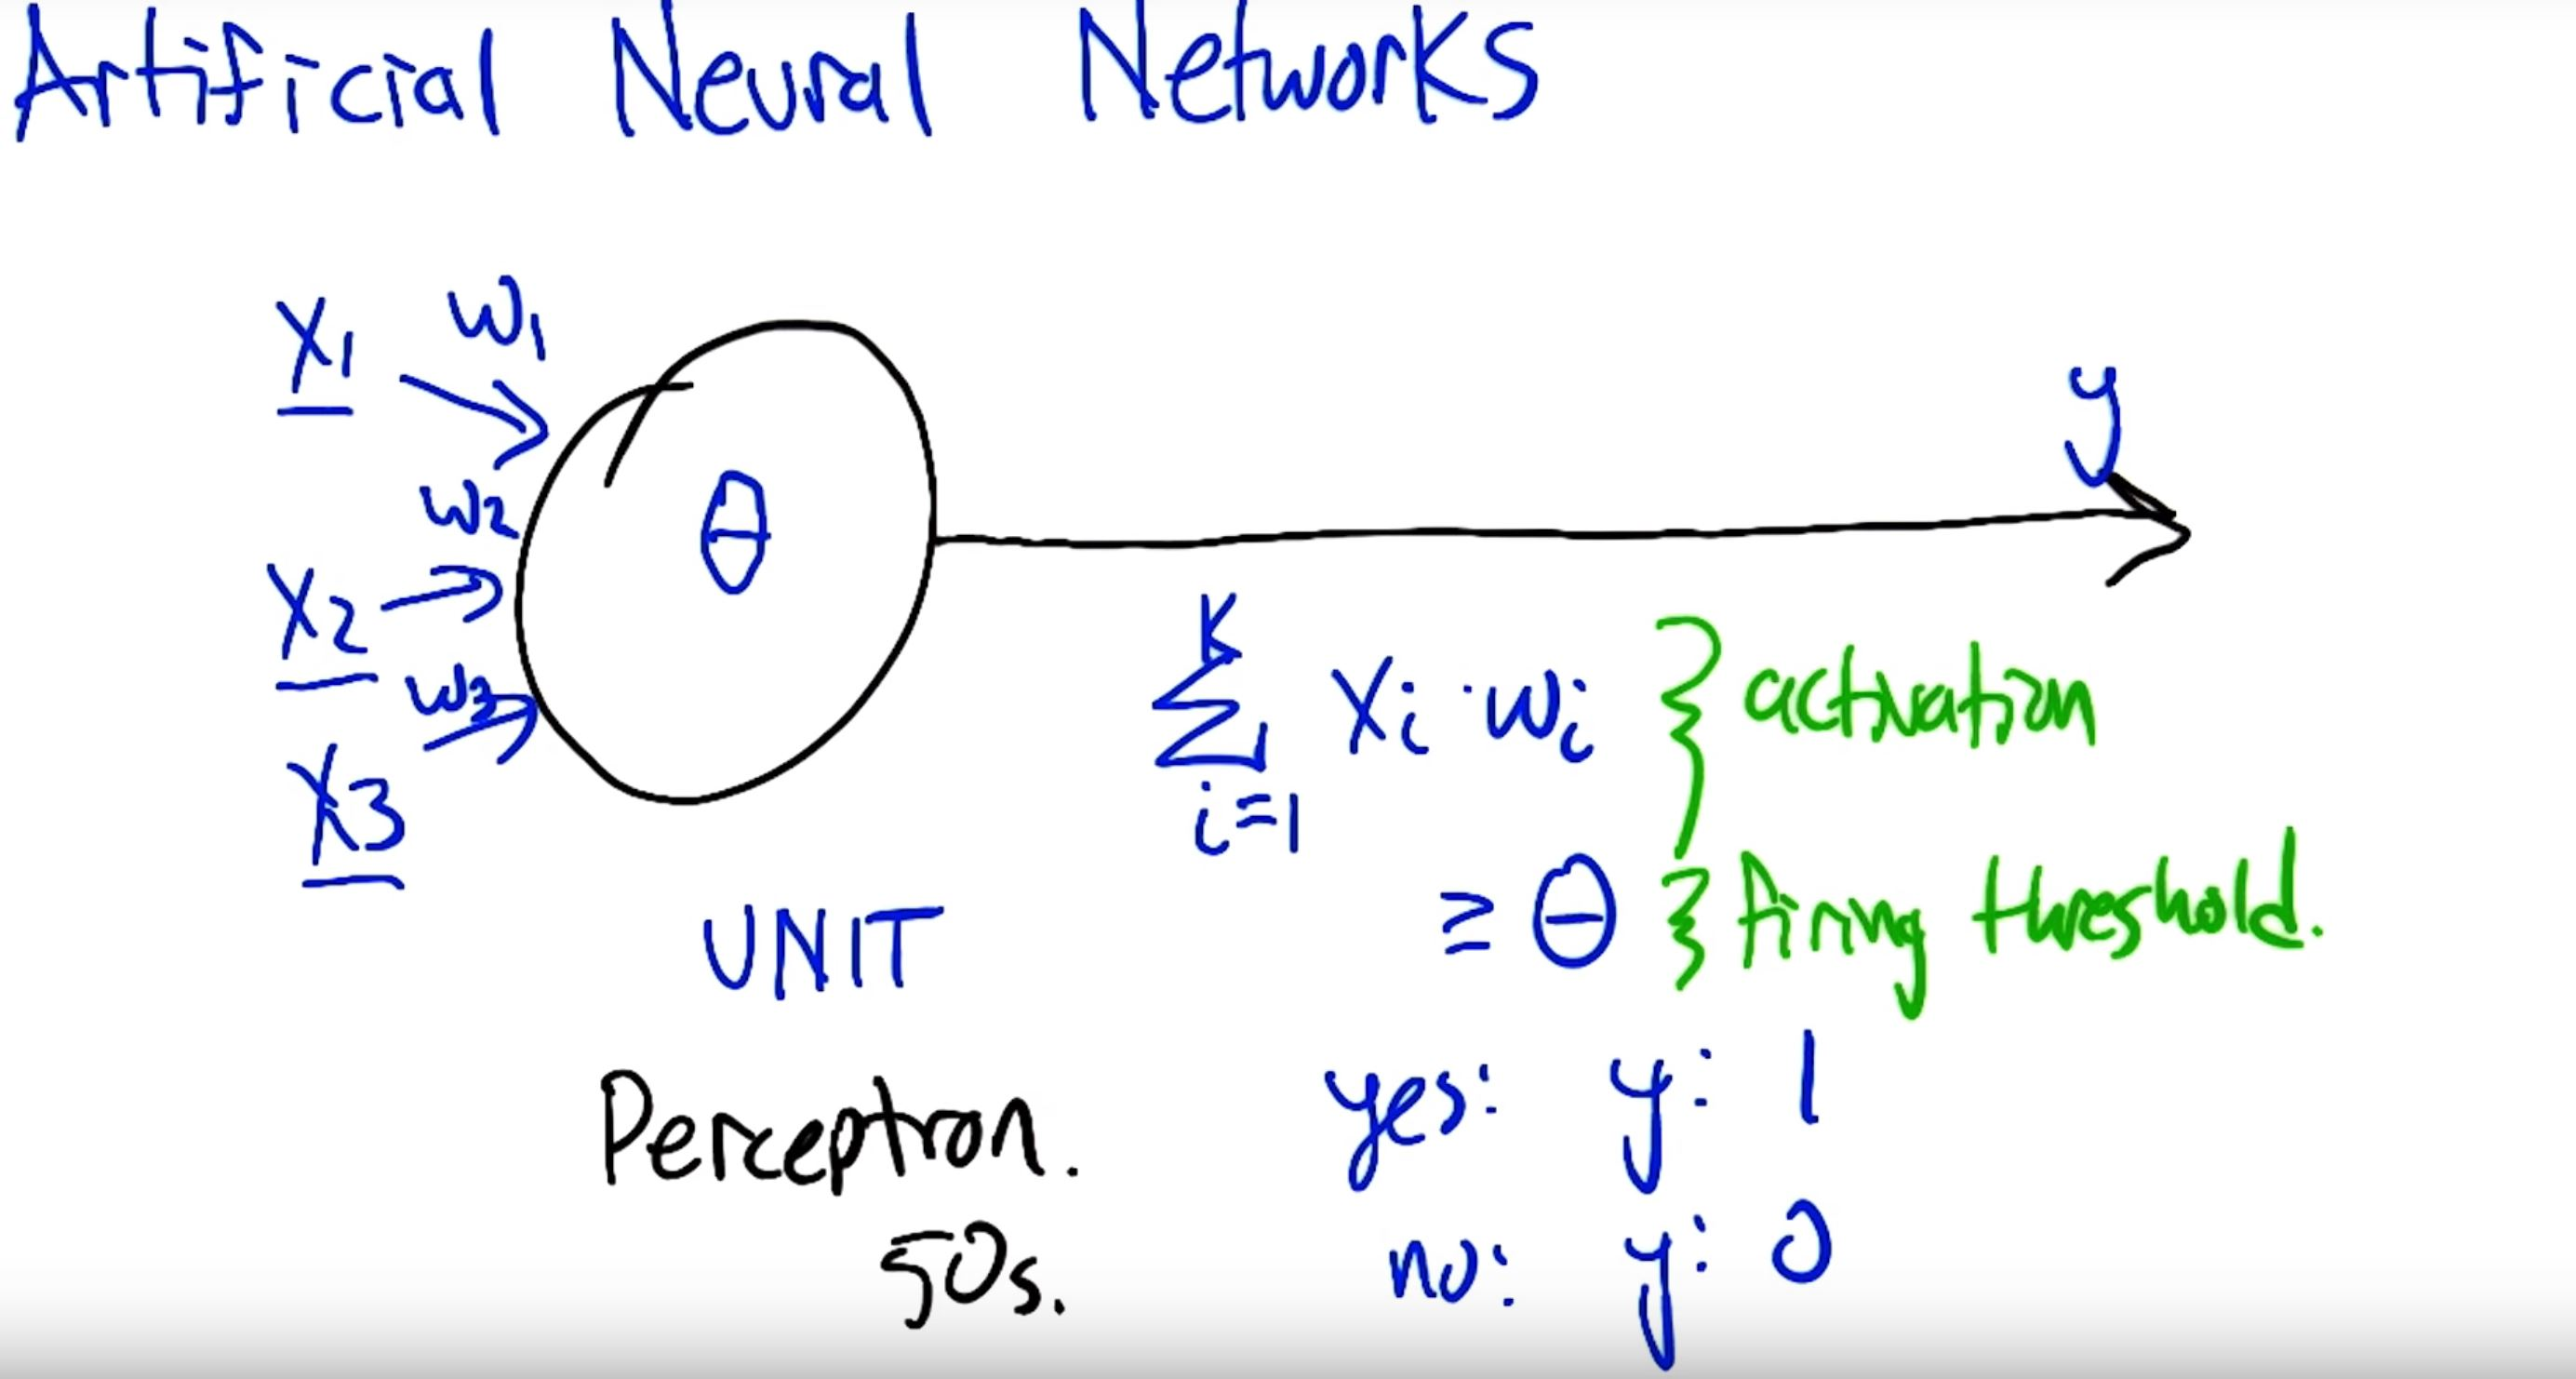
\includegraphics[width=0.5\textwidth]{pics/perceptron}
	\caption{Perceptron} 
	\label{perceptron}
\end{figure}
%         --------------------------------------

'And', 'or' or 'not' are all expressible as perceptron units \ref{and_or_perceptron}\footnote{One may go from the AND to the OR perceptron by increasing weights and/ore decreasing the bias.} - but 'Xor' is not (but $Xor = or - 2 * and$). 
%          --------   FIGURE: percepton  logical expressions -----------
\begin{figure}[htbp] 
	\centering
	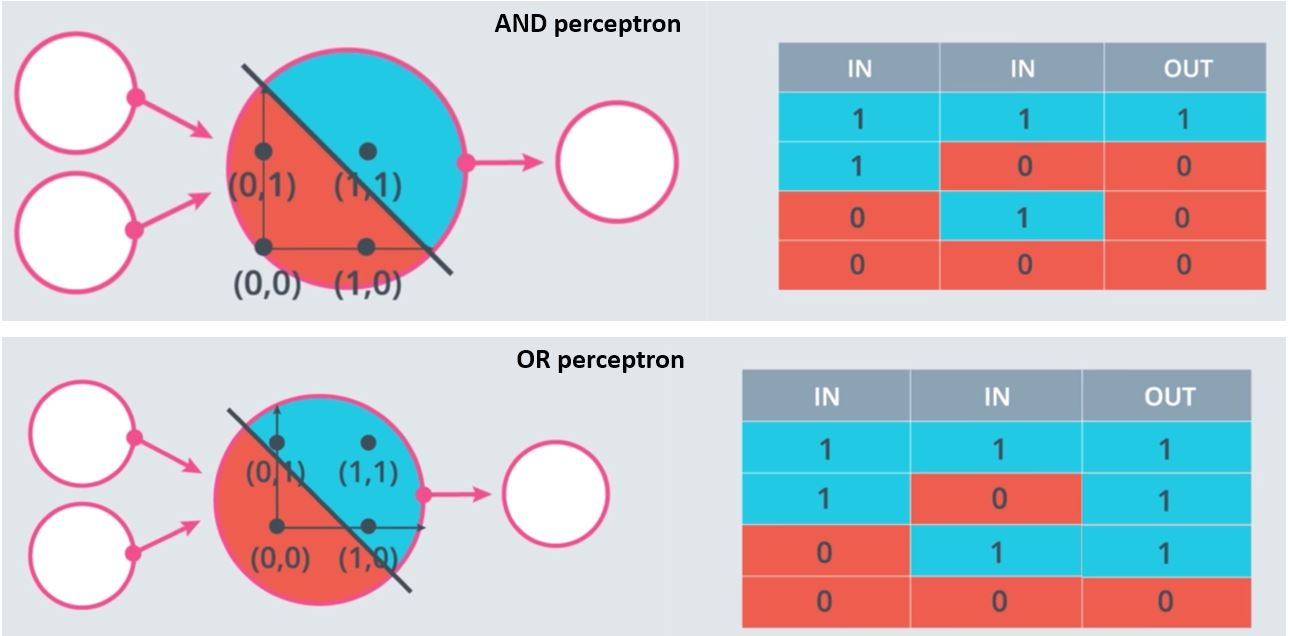
\includegraphics[width=0.6\textwidth]{pics/and_or_perceptron}
	\caption{AND, OR - Perceptron} 
	\label{and_or_perceptron}
\end{figure}
%         --------------------------------------

%          --------   FIGURE: percepton  algo -----------
% \begin{figure}[htbp] 
% 	\centering
% 	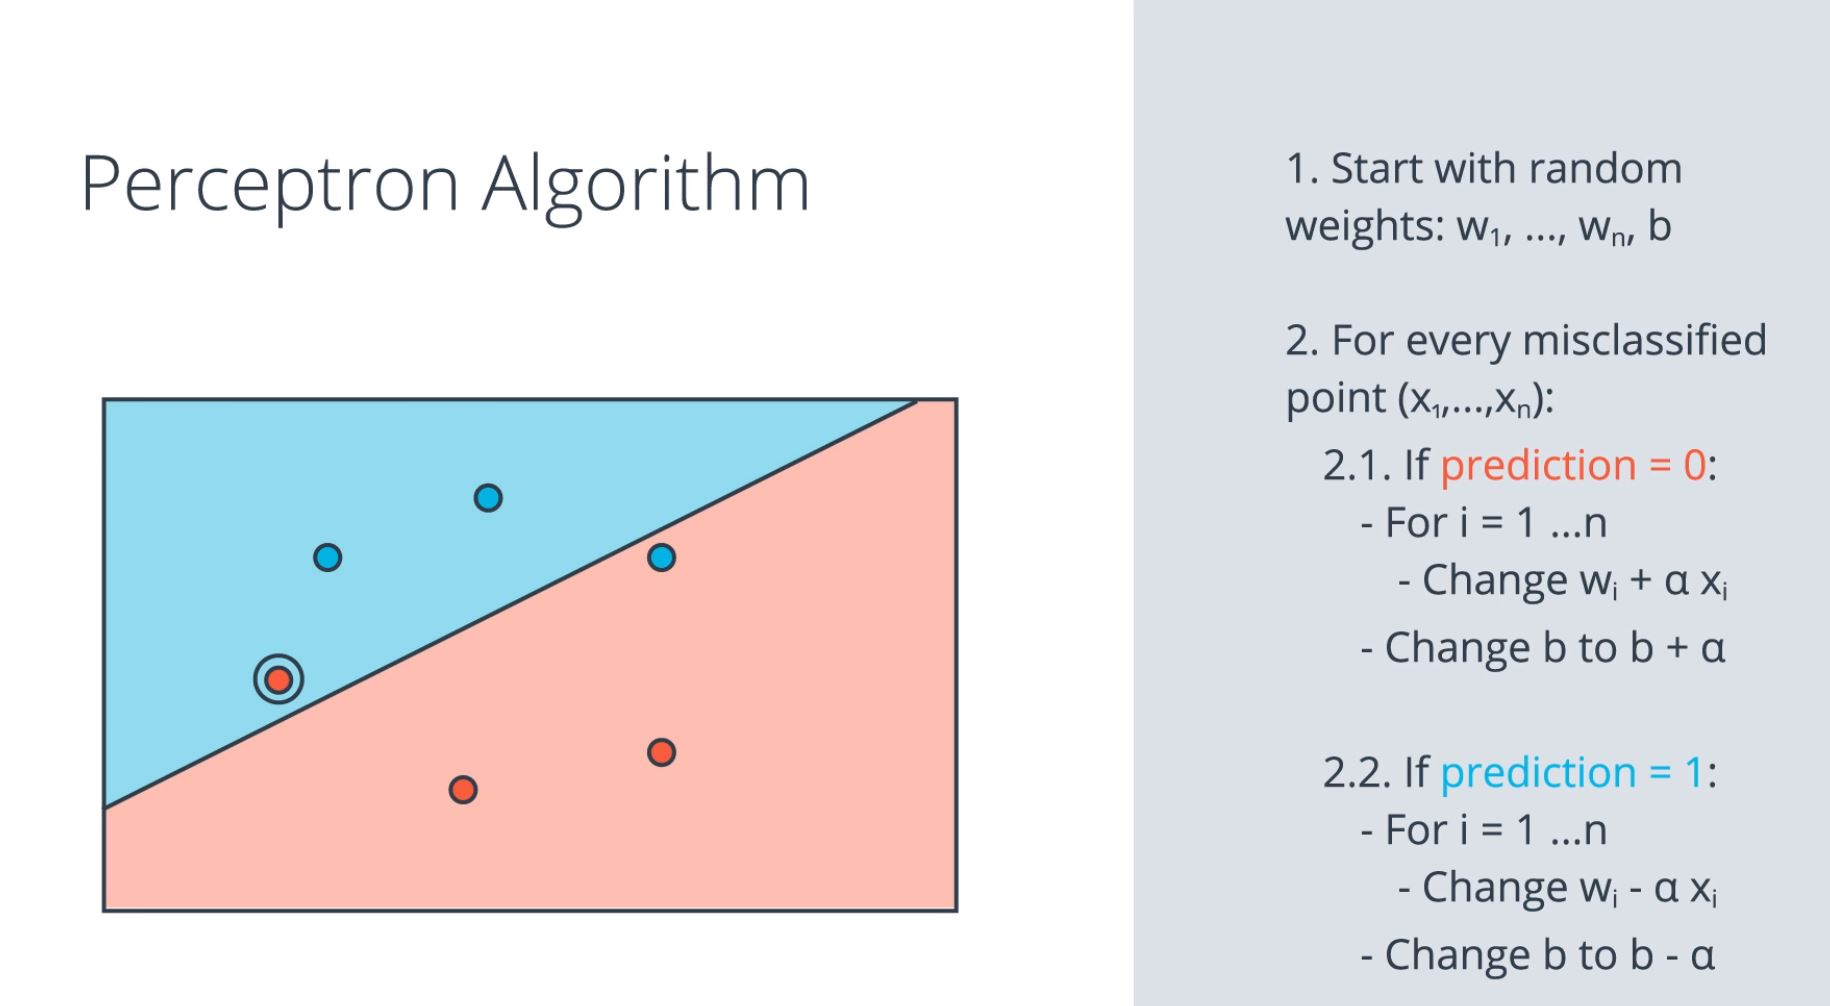
\includegraphics[width=0.7\textwidth]{pics/perceptron_algo}
% 	\caption{Perceptron algo} 
% 	\label{perceptron_algo}
% \end{figure}
%         --------------------------------------

\textbf{Rosenblatt}'s perceptron rules:
\begin{itemize}
	\item initialise weights to zero or small random numbers (reasons below);
	\item for each training sample/input: $x^{(i)}$:
	\begin{itemize}
		\item compute class output (using the step function)
		\item update weights: $w_j = w_j +  \underbrace{ \eta \, (y^{(i)} - predicted^{(i)}) x_j^{(i)}}_{\Delta w_j}$.
	\end{itemize}
\end{itemize}
where $\eta$ is the 'learning rate' in $(0., 1.]$. 

In words\footnote{Recall the two conventions: predictions and labels are (i) either 0 or 1, or alternatively (ii) either -1 or 1}: (i) if the point is correctly classified, do nothing. (ii) if the point is classified positive, but it has a negative (or zero) label, then reduce $w_j$ (ie $\Delta w_j$ is negative), (iii) if the point is classified negative (or zero), but it has a positive label, then increase $w_j$ (ie $\Delta w_j$ is positive).

The convergence of the perceptron is only guaranteed if the two classes are linearly separable\footnote{Xor (i.e. the Latin 'aut aut') is not linearly separable - represent such operator as done in fig. \ref{and_or_perceptron} to see.} and the learning rate is sufficiently small. Otherwise, it will never stop to update the weights. 
\begin{lstlisting}
# relevant part of a class
# X : {array-like}, shape = [n_samples, n_features]
# y : array-like, shape = [n_samples], Target values.

rgen = np.random.RandomState(self.random_state)
self.w_ = rgen.normal(loc=0.0, scale=0.01,
		   size = 1 + X.shape[1]) # 1 for 'bias unit'
self.errors_ = []
for _ in range(self.n_iter):  # limit iterations (e.g 50)
	errors = 0
	for xi, target in zip(X, y):	# loop through n_samples
		# xi is a vector of n_features
		net_input = np.dot(xi, self.w_[1:]) + self.w_[0]
		predict=np.where(net_input>=0.0, 1, -1) # unit step
		update = self.eta * (target - predict)
		self.w_[1:] += update * xi
		self.w_[0] += update
		errors += int(update != 0.0)
	self.errors_.append(errors)
return self
\end{lstlisting}
If all the weights were initialized to zero, the learning rate parameter $\eta$ would only affect the scale of the weight vector, not the direction (i.e. angle between vectors, via dot product, would be zero: 0. = np.arccos( v1.dot(v2) / (np.linalg.norm(v1) * np.linalg.norm(v2)) ).

Note that the prediction above is using a \textbf{step} function (predict is either 0 or 1, or -1 and 1); an alternative it is to use a logistic regression that would return a probability of each point being in one class.

\subsubsection*{Adaline}
ADAptive LInear NEuron (\textbf{Adaline}), by Widrow and Hoff. The key difference vs. the perceptron is that the weights are updated using a linear activation function instread that by a unit step fnct. In short, instead of comparing the target (true class) with the predicted class, Adaline compares the true class with the linear activation fnct value (which is here the identity fnct of the net input: $\phi(w^T x) = w^T x$, i.e. a real number). The advantageis that the linear activation fnct is \textit{differentiable} and convex. We can therefore use an objective fnct, in case of Adaline a SSE between true class and prediction that can be minimised:
\[ J(w) = \frac{1}{2} \sum_i (y^i - \phi(w^i \, x^i))^2
\] 
The term $1/2$ is used to make result easier. We can update the weights by taking a step in the opposite direction of the gradient $\nabla J(w)$ multiplied by the learning rate, i.e. $\Delta w = -\eta \nabla J(w)$ (to compute the gradient we take the partial derivative of SSE with respect to each weight $w_j$):
\[ 
w_j = w_j +   \eta \, (y^{(i)} - \phi(w^i \, x^i)) x_j^{(i)}
\]
The rule seems identical, but $\phi$ is a real number and not an integer class, furthermore weights update is calculated on \textit{all} samples in the training set (instead than incrementally after each sample like in the perceptron), which is why this approach is called \textbf{batch gradient descent}.

\begin{lstlisting}
rgen = np.random.RandomState(self.random_state)
self.w_ = rgen.normal(loc=0.0, scale=0.01,
			size=1 + X.shape[1])
self.cost_ = []
for i in range(self.n_iter):
	net_input = net_input(X)
	output = activation(net_input)  # identity here
	errors = (y - output)
	self.w_[1:] += self.eta * X.T.dot(errors)  # gradient on all training set
	self.w_[0] += self.eta * errors.sum()  
	cost = (errors**2).sum() / 2.0
	self.cost_.append(cost)
return self

def net_input(self, X):
    return np.dot(X, self.w_[1:]) + self.w_[0]

def activation(self, X):
    return X

def predict(self, X):
    """Return class label after unit step"""
    return np.where(activation(net_input(X)) >= 0.0, 1, -1)
\end{lstlisting}
We have to choose $\eta$ and $self.n\_iter$ - our \textbf{hyperparameters}- to minimise the $self.cost$ above.

Many learning algos, like gradient descent, benefits from features scaling: $x^{'}_j = 
(x_j - \mu_j) / \sigma_j$
\begin{lstlisting}
X_std = np.copy(X)
X_std[:,0] = (X[:,0] - X[:,0].mean()) / X[:,0].std()
\end{lstlisting}

A more computational efficient alternative to batch gradient descent (e.g. for millions of data points) is (online or) \textbf{stochatic gradient descent},. Recall that gradient descent loss function (i.e. objective fnct to be minimised needs to be \textit{continuous} - otherwise we'll get stuck if discrete - and differentiable). Please see appendix \ref{gradient_descent} for more details.

%%%%%%%%%%%%%%%%%%%%%%%%%%%%%%%%%%%%%%%%%%%%%%%%%%%%%%
\subsection{Softmax or Multinominal logit} \label{multinominal} 
Softmax has a variety of alternative names (e.g. multinominal logistic regression); this is a generalisation of the logistic regression or the perceptron with a sigmoid function as activation function to classify \textbf{more} than just two \textbf{classes}.

Every score (the higher, the better) can be turned into a probability:
\[ \text{Prob(class i}) = \frac{e^{z_i}}{e^{z_1} + \ldots + e^{z_n}}
\]
\begin{lstlisting}
def softmax(score_list):
    expL = np.exp(L)
    return expL / sum(expL)
\end{lstlisting}

Recall to apply One-Hot Encoding to assign a number to each different class (dummy) and avoid spurious dependency.

The algo to find such class probabilities is to maximising their maximum likelihood (product of the probabilities given the data) - but that tends to be a very small numbers for lots of probabilities / data points, we can therefore recast the problem in terms of the sum of the negative\footnote{Since a number in $(0, 1]$ has a negative log.} logarithm of each probability. Such sum is called \textbf{cross-entropy} and our goal is to minimise it (given the minus in front of $log$).

For two classes, cross-entropy is $ - [ \sum_{i=1}^m y_i \ln(p_i) + (1-y_i) \ln(1-p_i) ]$, where $y_i$ is either $0$ or $1$ for that point $i$, and $m$ is the number of datapoints.

In case of \textbf{logistic regression}, indeed, we have that the (average) error function is:
\[ E = -\big( \frac{1}{m} \sum_{i=1}^m y_i \ln(\sigma(w x^{(i)}+b)) + (1-y_i) \ln(1-\sigma(w x^{(i)}+b)) \big) 
\]  
where $\sigma(z)$ is the sigmoid function for  $z = w x^{(i)}+b$ (in other words, $p_i$ is the sigmoid - sometimes indicated also as $\hat{y}$ - to stress the fact that is a prediction besides a probability).

For more classes, the \textbf{multi-class cross-entropy} (also called 'error function' if averaged over $m$):
\[ \text{X-Entropy} =  -\sum_{j=1}^n \sum_{i=1}^m y_{ij} \ln(p_{ij})
\]
where $n$ is the number of classes and $y_{ij}$ is $1$ if event occurred and zero otherwise (dummy variable). 


\subsubsection*{Gradient aside}
Let's recall the error formula for two-classes case (and re-writing using $\hat{y}$ to indicate the sigmoid function):
\[ E = - \frac{1}{m} \big( \sum_{i=1}^m y_i \ln(\hat{y}_i) + (1-y_i) \ln(1-\hat{y}_i) \big)
\]  
where $\hat{y}_i$ = $\sigma(w x^{(i)}+b) = 1 / (1+e^{-(w x^{(i)}+b)}) $ and that its derivative is rather simple:
\[ \sigma'(z) = \frac{\partial}{\partial z} \frac{1}{1+e^{-z}} 
= \frac{e^{-z}}{(1+e^{-z})^2} =
\frac{1}{(1+e^{-z})} \frac{e^{-z}}{(1+e^{-z})} = \sigma(z) (1-\sigma(z))
\]

We want to calculate the gradient of $E$ at point $x=(x_1, \ldots, x_n)$:
\[ \nabla E = (\frac{\partial E}{\partial w_1}, \ldots, \; \frac{\partial E}{\partial b}, \frac{\partial E}{\partial w_1} )
\] 
To simplify our calculations, we'll actually think of the error that each point produces, and calculate the derivative of this error. The overall error is, then, the average of the errors at all the points. For a single point $x$ with respect to weight $w_j$ we have:
\begin{align*}
\frac{\partial E}{\partial w_j}  &= \frac{\partial}{\partial w_j} [ -y \ln(\hat{y}) - (1-y) \ln(1-\hat{y})] \\
&= -\frac{y}{\hat{y}} \underbrace{\frac{\partial \hat{y}}{\partial w_j}}_{\hat{y}(1-\hat{y})x_j}  - \frac{1-y}{1-\hat{y}} \underbrace{\frac{\partial (1-\hat{y})}{\partial w_j} }_{-\hat{y}(1-\hat{y})x_j} \\
&= -(y-\hat{y}) x_j
\end{align*}
and, similarly, 
\[\frac{\partial E}{\partial b} =  -(y-\hat{y}) 
\]
In summary, for a point $(x_1, \ldots, x_n)$, label $y$ and prediction $\hat{y}$,  the gradient of the error function for that point is:
\[ \nabla E = -(y-\hat{y})  (x_1, x_2, \ldots, 1)
\]
i.e., the gradient is a scalar times the coordinates of the point: the closer the label to the prediction, the smaller the gradient and vice-versa.

Note similarity with the perceptron update algorithm in section \ref{perceptrons}) - only difference is that $\hat{y}$ is either zero or 1 in the perceptron, but a number between zero and 1 (probability) for the gradient descent (so doing nothing is practically never an option for the latter: misclassified points gets closer to the boundary line, as per the perceptron, but correctly classified gets pushed further away from the boundary line, contrarily to the perceptron where nothing happens).

Since the \textbf{gradient descent step} consists in \textit{subtracting a multiple of the gradient} of the error function at every point, the updated weights are:
\[ w^{new}_i \leftarrow \; w_i \underbrace{- \frac{\alpha}{m} [-(y-\hat{y}) x_j]}_{+\frac{\alpha}{m} (y-\hat{y}) x_j}
\]
and similarly for the bias $b^{new}_i \leftarrow \; b_i + \alpha/m \cdot (y-\hat{y})$.

Recall that $\alpha/m$ is our \textit{learning rate}, which is a constant.

Gradient descent: initial weights are generally small random values; random to avoid local minima by introducing variability, small for lower complexity because big weights may lead to over-fitting.

%%%%%%%%%%%%%%%%%%%%%%%%%%%%%%%%%%%%%%%%%%%%%%%%%%%%%%
\subsection{Support Vector Machines}
Separate data using hyperplane (a line in 2-dim, a plane in 3-dim, ...), intuitively the best line is the one least committed to the data (not too close to one of the classes in our training data), or in other words, the one that maximises the distance between the nearest points of the classes and the line/hyperplane, that distance is called \textbf{margin} in SVM (the idea is that of robustness: we use the training data, but we don't trust them too much - so we keep equidistant).
%          --------   FIGURE: SVM  -----------
\begin{figure}[htbp] 
	\centering
	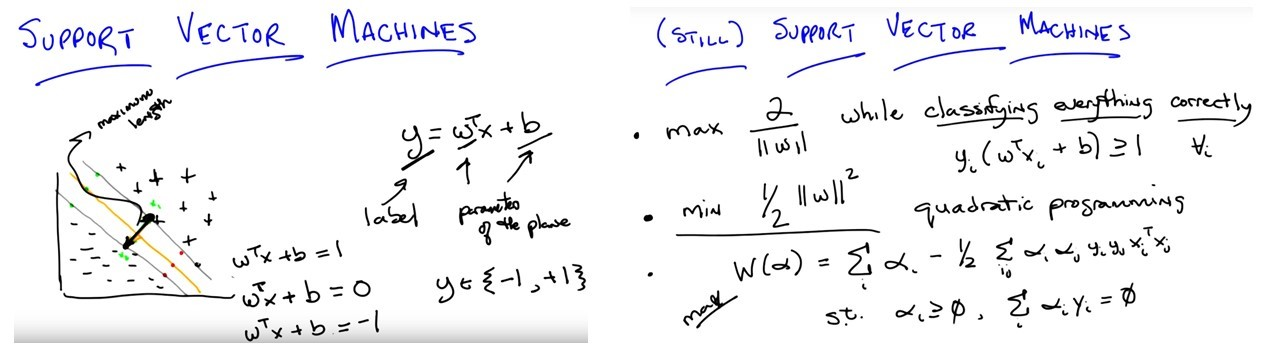
\includegraphics[width=1.\textwidth]{pics/SVM}
	\caption{SVM} 
	\label{SVM}
\end{figure}
%         --------------------------------------

In order to maximise such distance, we can subtract the two boundaries from one another (see left-hand side fig. \ref{SVM}) and be left with $w^T (x_1-x_2) = 2$, then divide by the norm of $w$. Hence we need to maximise $2 /||w|| $ subject to $y_i (w^T x_i + b) \geq 1 ;\forall i$ (note that we multiply by $y_i$ to avoid writing two inequalities for $(\dots)$ $\leq -1$ and $\geq 1$ ). 
An equivalent, but easier (quadratic: unique solution) problem is to minimise $ ||w||^2 /2$ with same constraints - that again can transform into another quadratic problem with $alpha$ as new param(s) (see right-hand side fig. \ref{SVM}). We can then recover $w$ simply as $w=\sum_i \alpha_i y_i x_i$ and since most of alphas are zero, one only needs a few of $x_i$ matter (you can see intuitively in a plane that the $x_i$ closer to the separating line matter).

We can use the \textbf{kernel trick} (adding one or further dimensions) to separate classes linearly with an hyper-plan - see fig. \ref{kernel_trick}, the kernel is the transformation we are applying to the dot product ($x_i x_j$) in fig \ref{kernel_trick}. Besides $k = (x^T y)^2$ in the fig (called '\textit{linear}'), there are many other possible transformations like the gaussian-looking '\textit{rbf}' $k(x,y)= \exp(-\gamma ||x-y||^2)$) or the \textit{sigmoid} $\tanh(\alpha x^y y + \theta)$. A Kernel must satisfy the \underline{Mercer condition}, i.e. intuitively it must act as a distance/inner product\footnote{The kernel trick avoids the \textit{explicit} mapping that is needed to get \textit{linear} learning algorithms to learn a \textit{nonlinear} function or decision boundary. For all x and y in the input space, certain functions $k(x,y)$ can be expressed as an inner product in another space - the $k$ map is called \textit{kernel} (the word 'kernel' is generally used in mathematics to denote a weighting function for a weighted sum or integral).}. 

%          --------   FIGURE: Kernel trick  -----------
\begin{figure}[htbp] 
	\centering
	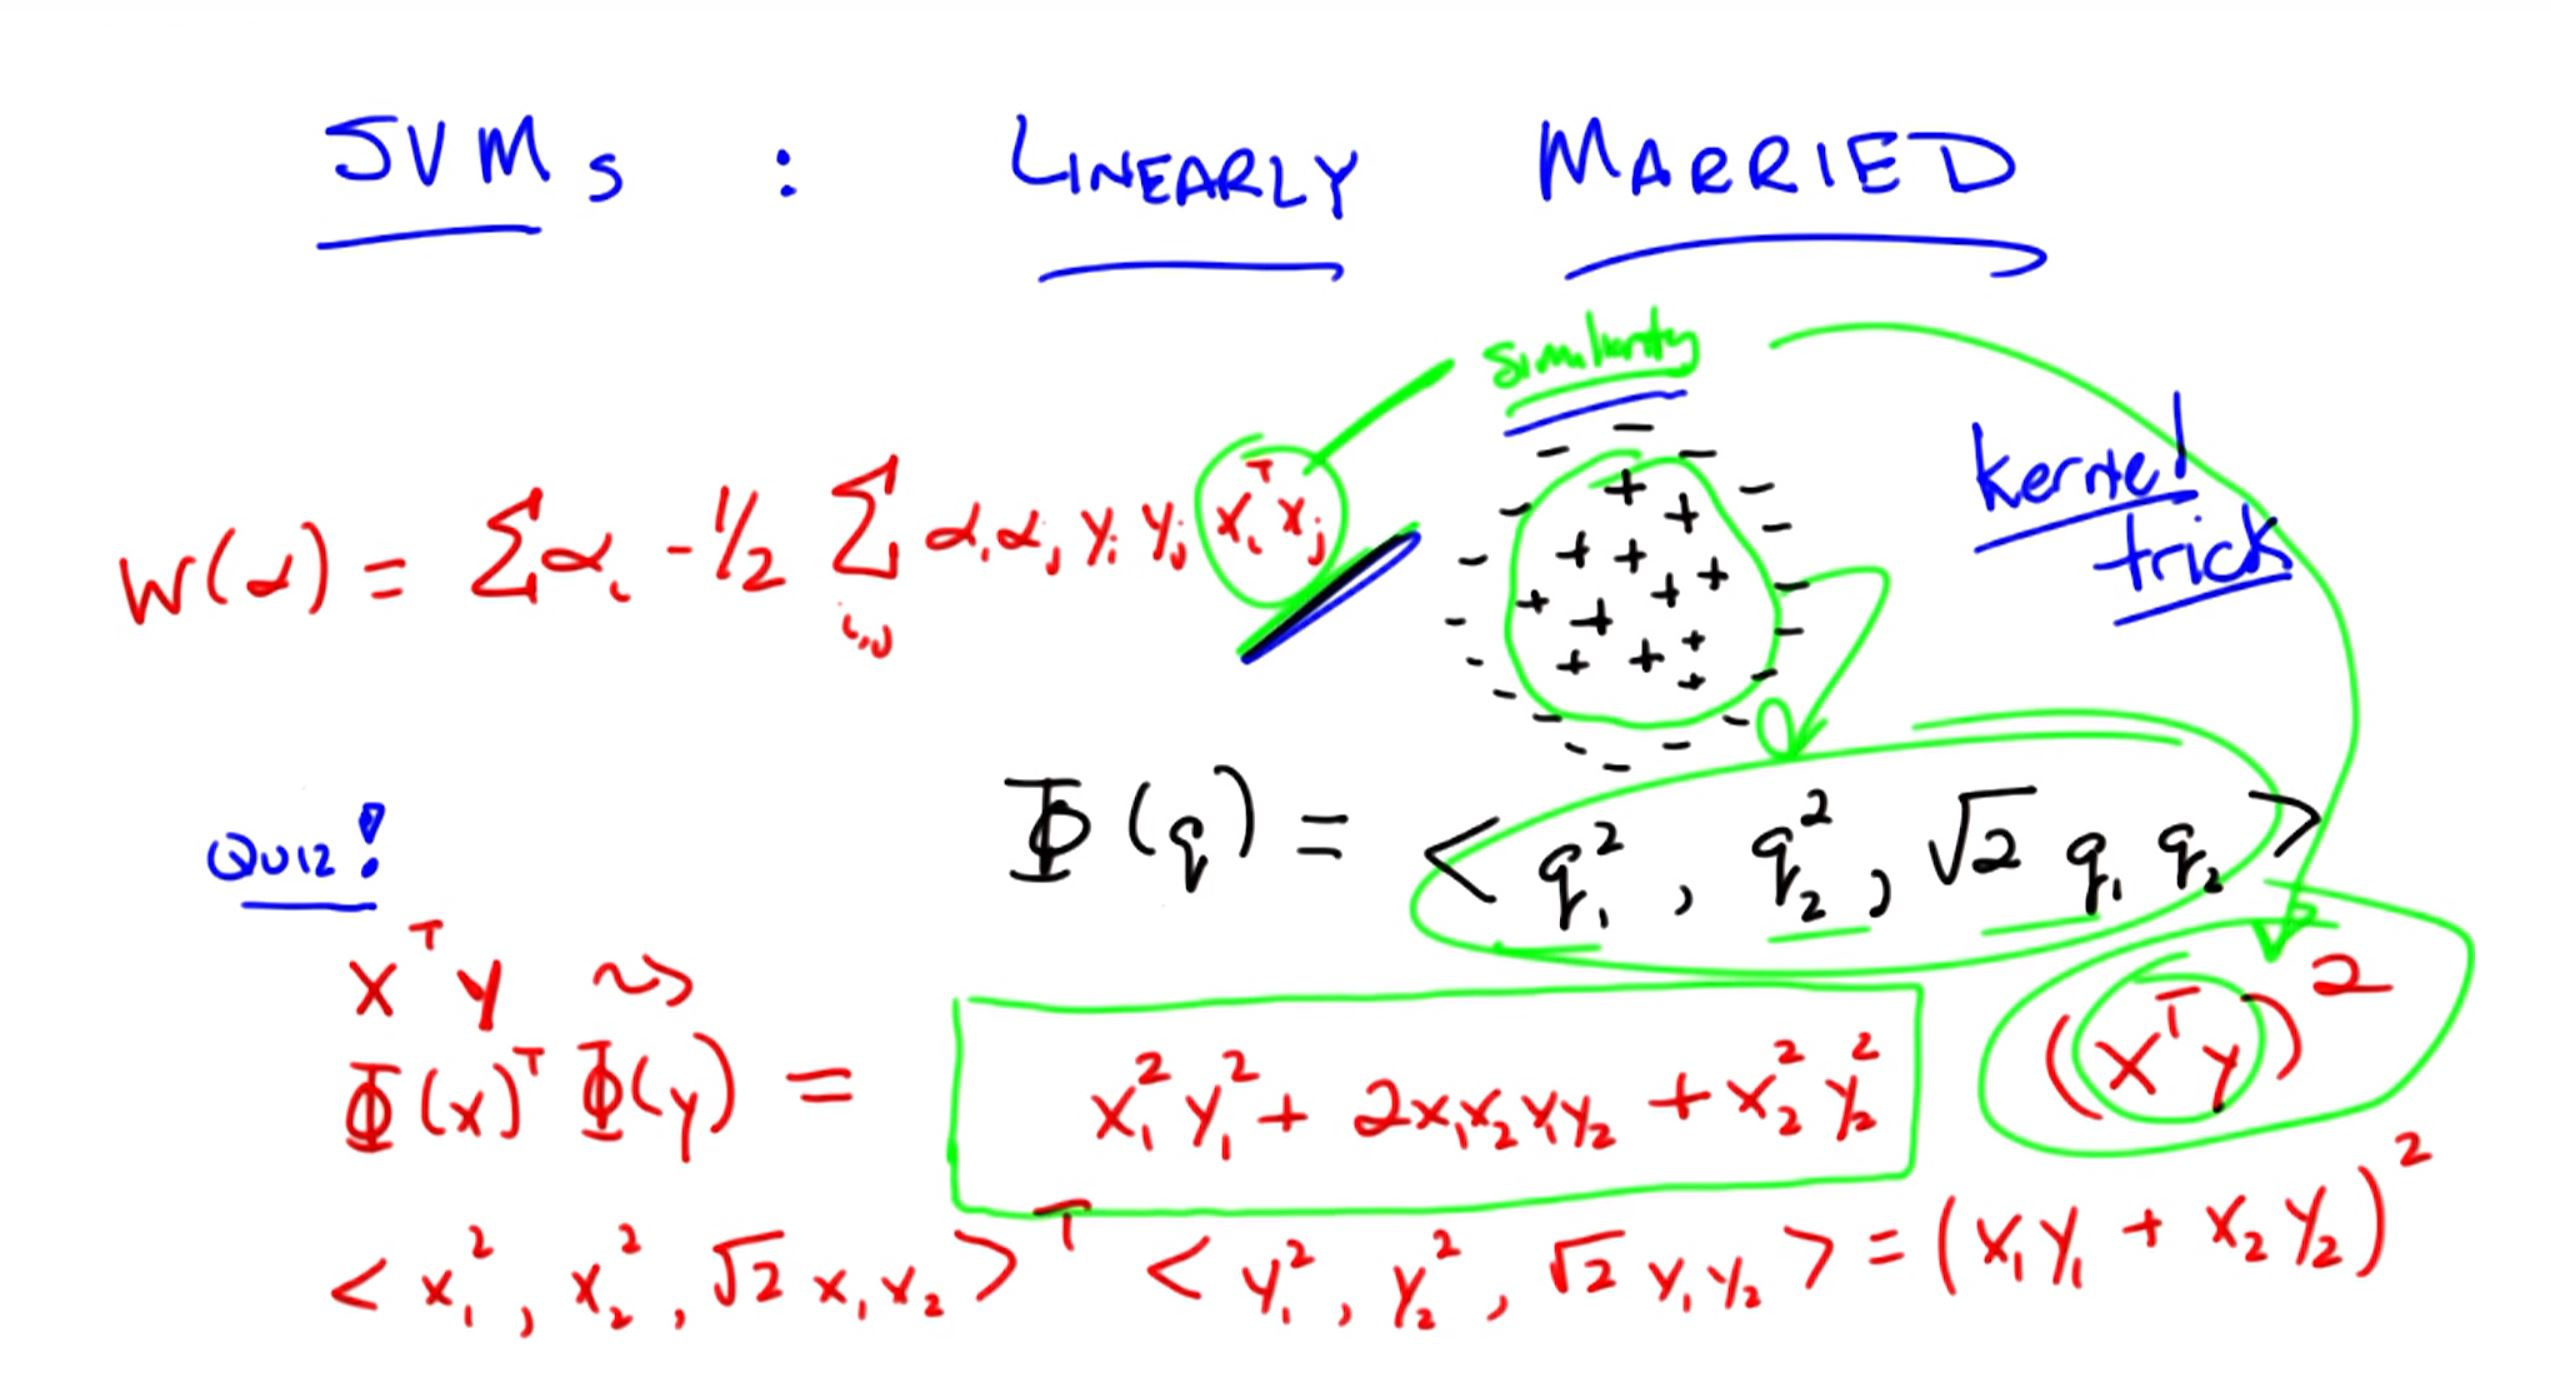
\includegraphics[width=.9\textwidth]{pics/kernel_trick}
	\caption{Kernel trick (SVM)} 
	\label{kernel_trick}
\end{figure}
%         --------------------------------------


Coding example using a built-in dataset:
\begin{lstlisting}
# 1. get data
from sklearn.datasets import load_breast_cancer
cancer = load_breast_cancer()

cancer.keys() # data shown in dict keys
# -> dict_keys(['DESCR', 'target', 'data', 'target_names', 'feature_names'])
print(cancer['DESCR'])  # long description
 
 #set-up df of the features and target
df_feat = pd.DataFrame(cancer['data'], 
					columns=cancer['feature_names'])
df_target = pd.DataFrame(cancer['target'], columns=['Cancer'])

# 2. do some explanatory data analysis
# e.g. sns.pairplot with hue = target

# 3. S V Classifier
 # train split
from sklearn.model_selection import train_test_split
X_train, X_test, y_train, y_test = 
	train_test_split(df_feat, df_target, 
	test_size=0.30, random_state=101)
	
  # build 'naive' SVC: WRONG WAY
from sklearn.svm import SVC
model = SVC()
model.fit(X_train,y_train)
predictions = model.predict(X_test)

 # evaluate
from sklearn.metrics import classification_report,confusion_matrix
print(confusion_matrix(y_test,predictions))
print(classification_report(y_test,predictions))
# all classficed into a single class... we need GridSearch

 
 # build SVC properly: use GridSearch (meta-estimator)
from sklearn.model_selection import GridSearchCV
param_grid = {'C': [0.1,1, 10, 100, 1000], # is C not gamma? CHECK!!!
	'gamma': [1,0.1,0.01,0.001,0.0001], 'kernel': ['rbf']}  
grid = GridSearchCV(SVC(),param_grid,refit=True,verbose=3)	
              , # scoring=make_scorer(fbeta_score, beta=0.5))
# rbf: this is actually default, get verbose>0 to see some output
grid.fit(X_train,y_train)  # May take awhile!
grid.best_params_    # show best params
grid.best_estimator_ # show best estimator
grid_predictions = grid.predict(X_test)

 # evaluate (will be much better than naive one above)
print(confusion_matrix(y_test,grid_predictions))
print(classification_report(y_test,grid_predictions))
\end{lstlisting}
Besides the \textbf{Kernel} (linear, poly, rbf which is the default, sigmoid, or even a custom one), there are two more params: (i) \textbf{C}, the penalty parameter of the error term (it controls the tradoff between \textit{smooth} decision boundary and classifying training points \textit{correctly}: the lower the smoother the boundary, the higher the more correct) and (ii) \textbf{gamma} (coefficient for ‘rbf’, ‘poly’ and ‘sigmoid’ - hence no effect on the 'linear' kernel; it can be seen as the inverse of the radius of influence of samples selected by the model as support vectors; too large and it will overfit, too small and it will be too constrained).

NB: you can use \textit{StratifiedShuffleSplit}, rather than GridSearchCV, to ensure that training and validation sets have approximately the same number of data points of each output class, which is particularly useful with the imbalance in class labels.

%%%%%%%%%%%%%%%%%%%%%%%%%%%%%%%%%%%%%%%%%%%%%%%%%%%%%%
\subsection{Ensembles}
You get some simple rules and combine them to get a complex rule (learn over a subset of data that generates a rule, repeat, and combine all).

%
\subsubsection{Bagging}
\textbf{Bagging or Bootstrapping aggregation}: combine simple rule(s) (e.g. 3rd order polynomial) on \textbf{random subsets} of the training data and average the result. 

Bagging is the simplest ensemble learning we can think of: 
\begin{itemize}
	\item Simplest way to choose data: select uniformly randomly subsets.
	\item Simplest combination: simple average.
\end{itemize}

Such an ensemble learning tends to perform \underline{better on the test/validation} datasets (lower variance) than more complex models (e.g. a 4rd order polynomial fitted on all training data, which obviously fits better: lower bias).

Note that Random Forests are related to Bagging (averaging across trees to reduce variance), but with an extra randomness added by sub-sampling features.

%
\subsubsection{Boosting}
Let's improve on Bagging by (i) focusing on the \textbf{'hardest'} examples and using (ii) \textbf{weighted} mean.

Introducing a new error definition (rather than simple mismatch) as probability - given a distribution - that my Hp disagrees with the truth concept on some instances $x$ : $Pr_{distr}[Hp(x) \neq c(x)]$. 

Concept of \textbf{weak learner}: no matter the distribution of the data, it gets lower errors than chance (e.g. $<0.5$): prob above is $ \ldots \leq 0.5 - \epsilon$.

%          --------   FIGURE: Boosting  -----------
\begin{figure}[htbp] 
	\centering
	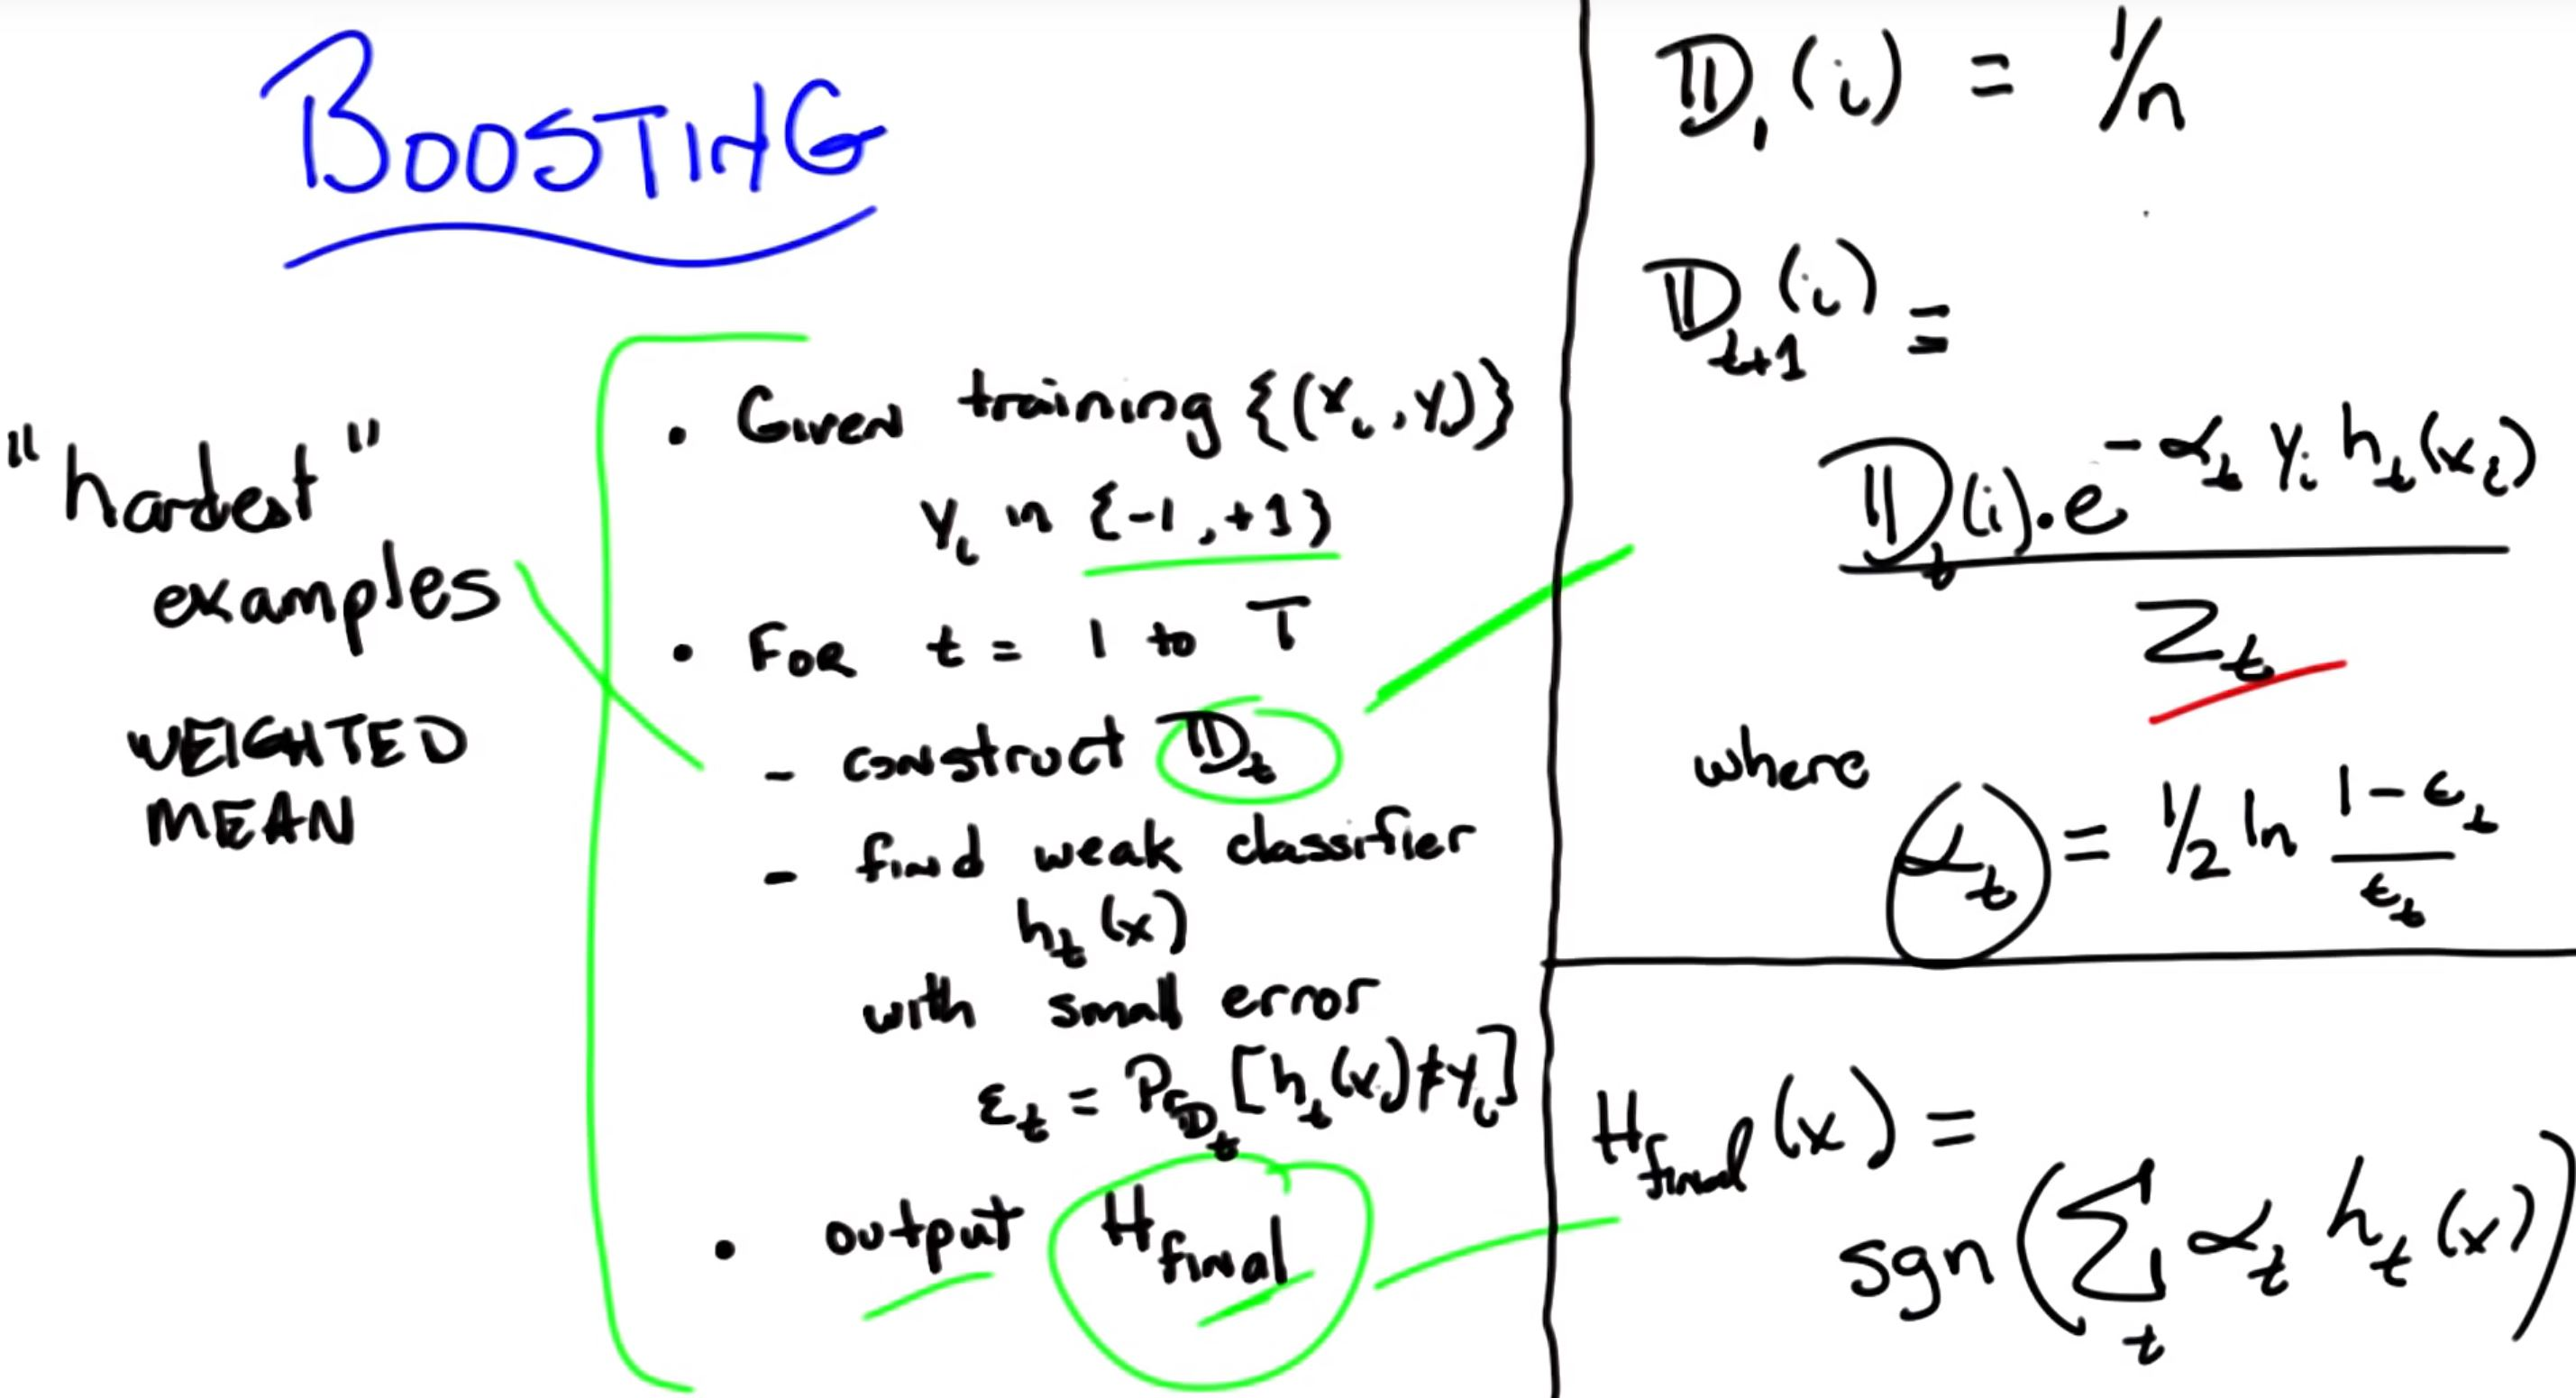
\includegraphics[width=.9\textwidth]{pics/boosting_1}
	\caption{Boosting algorithm} 
	\label{boosting_1}
\end{figure}
%         --------------------------------------
In fig. \ref{boosting_1}: note that if $y_i$ and $h_t(x_i)$ agrees (i.e. both $+1$ or $-1$), considering that $alpha$ is positive, the single $D_{t+1}(i)$ decreases (but the whole $D_{t+1}$ depends on other $x_i$). The final $H_{final}$ is a weighted function of the $h$ (if you divide by $sum_i \alpha_i$, that becomes a weighted average and result remains the same): as we keep adding more and more learners, the error may not decrease much - but our confidence increases (more certain about harder example - we increase the margin), which helps avoiding overfitting. Boosting is agnostic to the learner, as long as a 'weak' learner (better than 50%).

Boosting may overfit if (i) the underlying learner overfits from the start (e.g. ANN with many layers) any looping does not make it better, (ii) 'pink noise' (uniform noise). 

%%%%%%%%%%%%%%%%%%%%%%%%%%%%%%%%%%%%%%%%%%%%%%%%%%%%%%
%	UNSUPERVISED LEARNING
%%%%%%%%%%%%%%%%%%%%%%%%%%%%%%%%%%%%%%%%%%%%%%%%%%%%%%
\section{Unsupervised learning}
We will review a few clustering methods - starting from the simple one, than the most popular one, and finally one that solves some of the limitations of the latter (non globular data) - and a dimensionality reduction technique (PCA).

Good properties of a clustering scheme are (i) richness (i.e. every partition should be possible), (ii) scale invariance (i.e. not sensitive to changes in the units of distance measurement) and (iii) consistency (i.e.by reducing distances within the clusters and enlarging between the clusters then we still have the same clustering).
However, you cannot have all the three properties in a clustering algorithm since they are contradictory (Impossibility Theorem of Kleinberg). You can get two of those.

%%%%%%%%%%%%%%%%%%%%%%%%%%%%%%%%%%%%%%%%%%%%%%%%%%%%%%
\subsection{Principal Component Analysis}
Principal Component Analysis (PCA) is an \textbf{unsupervised} learning algorithm (like K-Means Clustering). In short, PCA is a transformation of data (feature transformation) in attempts to find out which features explain the most variance in the data (graphically find the new axes). 

PCA helps us to identify patterns in data based on the correlation between features. In a nutshell, PCA aims to find the directions of maximum variance  (i.e. the \textbf{orthogonal} axes of the new subspace: principal components) in high-dimensional data (e.g. original dimensionality: $d$) and projects it onto a new subspace with fewer dimensions than the original one (new dimensionality: $k$, which is $<d$). Algo steps (from scratch):
\begin{itemize}
	\item Standardize the d-dimensional dataset;
	\item Construct the covariance matrix;
	\item Decompose the covariance matrix into its eigenvectors and eigenvalues;   
	\item Sort the (abs of) eigenvalues by decreasing order and select the corresponding $k$ (largest) eigenvectors;
	\item Construct a projection matrix $W$ from the "top" $k$ eigenvectors;
	\item Transform the $d$-dimensional input dataset $x$ using the projection matrix W to obtain the new (smaller) $k$-dimensional feature subspace.
\end{itemize}

\begin{lstlisting}
from sklearn.model_selection import train_test_split
X, y = df_wine.iloc[:, 1:].values, df_wine.iloc[:, 0].values
X_train, X_test, y_train, y_test = \
train_test_split(X, y, test_size=0.3, 
stratify=y, random_state=0)

# NB: if necessary: (i) normalise data first (i.e. log-transform)
#                  (ii) remove any outliers 
#     then		
# standardize the features
from sklearn.preprocessing import StandardScaler
sc = StandardScaler()
X_train_std = sc.fit_transform(X_train)
X_test_std = sc.transform(X_test)

import numpy as np
cov_mat = np.cov(X_train_std.T)
eigen_vals, eigen_vecs = np.linalg.eig(cov_mat)

# explained variance ratios
tot = sum(eigen_vals)
var_exp = [(i / tot) for i in
sorted(eigen_vals, reverse=True)]
cum_var_exp = np.cumsum(var_exp)
# ... etc ... 

# Make list of (eigenvalue, eigenvector) tuples and sort
eigen_pairs = [( np.abs(eigen_vals[i]), eigen_vecs[:, i] )
for i in range(len(eigen_vals))]
eigen_pairs.sort(key=lambda k: k[0], reverse=True)

# NB: [:, np.newaxis] make it a column vector
# and concatenate 
w = np.hstack((eigen_pairs[0][1][:, np.newaxis],
eigen_pairs[1][1][:, np.newaxis]))

# transform training dataset
X_train_pca = X_train_std.dot(w)  # = x W

\end{lstlisting}

By using sklearn we only need to perform the first step above (log-transform and removing outliers if necessary,  then standardise) - all other ones are hidden behind the $PCA()$ algo:
\begin{lstlisting}
# 1. Get the data
from sklearn.datasets import load_breast_cancer
cancer = load_breast_cancer()
cancer.keys()  # dict_keys(['DESCR', 'data', 
# 'feature_names', 'target_names', 'target'])
print(cancer['DESCR'])
df = pd.DataFrame(cancer['data'],columns=cancer['feature_names'])

# 2. PCA Visuation (but first scale data)
# NB: you should really fit scaler on training (good) data only
#     and then transform both (bad) training and test data as above
from sklearn.preprocessing import StandardScaler
scaler = StandardScaler() 
scaler.fit(df)
scaled_data = scaler.transform(df)

from sklearn.decomposition import PCA  # NB: .[family]
pca = PCA(n_components=2)  # instantiate
# NB: n_components=None  -> all components
pca.fit(scaled_data)  # find the components (fitting)
x_pca = pca.transform(scaled_data)  # rotation and dim reduction

# explained variance ratio (eigenvalues as %)
print(pca.explained_variance_ratio_)

# components (vectors)
first_pc = pca.components_[0]
second_pc = pca.components_[1]

scaled_data.shape  # e.g. (569, 30) vs. below
x_pca.shape  # (569, 2)  

plt.figure(figsize=(8,6))
plt.scatter(x_pca[:,0],x_pca[:,1], c=cancer['target'], cmap='plasma')
plt.xlabel('First principal component')
plt.ylabel('Second Principal Component')

# components stored as attributes
pca.components_

# each row in the matrix array above is a princ. component
# and each column related to orginal features
# We can visualize such relationship with a heatmap:
df_comp = pd.DataFrame(pca.components_,columns=cancer['feature_names'])
plt.figure(figsize=(12,6))
sns.heatmap(df_comp,cmap='plasma')
# color bar represents corr(feature, principal)
\end{lstlisting}
NB: the values for the first, say, two dimensions remains unchanged when compared to a PCA transformation in, say, six dimensions.

When to use PCA: (i) latent features driving the data patterns, (ii) dimensionality reductions (visualise high-dimension data, or reduce noise, or make other algo work better with fewer features). E.g. eigenfaces: recognise facial pics (having lots of pixels) using fewer points (since general common features: darkness, average face, etc.).

Unfortunately, with this great power of dimensionality reduction, comes the cost of being able to easily understand what these components represent (\textit{loss of interpretability}). The components correspond to combinations of the original features, the components themselves are stored as an attribute of the fitted PCA object.

%%%%%%%%%%%%%%%%%%%%%%%%%%%%%%%%%%%%%%%%%%%%%%%%%%%%%%
\subsection{Independent Component Analysis}
Whilst PCA finds correlations by maximising variance, Independent Component Analysis (ICA) is a linear transformation where (i) new features (components) are independent (and non-gaussian) and (ii) mutual information between new and original features is as high as possible. 

The blind source separation (or the cocktail party) problem: whilst recording simultaneous conversations in a party, we need to separate or focus on one particular person (people are the hidden variables, observables are the microphones but each has a different linear combinations of these persons' voices). This signal separation problem is the one that ICA is really good at solving. 

ICA is motivated by the idea that when you add things up, you get something normal, due to the central limit theorem, and really hopes that the data are non-normal, so that the non-normal components can be extracted from them. To exploit non-normality, ICA tries to maximize the fourth moment (Kurtosis) of a linear combination of the inputs (all considered equally relevant vs. PCA that ordered them). PCA, instead, maximizes the second moment (variance) of a standardized combination of inputs (getting mutually orthogonal features, and ordered features). Whilst eigenfaces (PCA applied to face recognition) finds brightness and average face as first two components (and works for reconstruction), ICA finds different components like nose, smile, hair, chin on bottom (and hence finds 'parts of'); for forests PCA finds something similar (brightness, ...), ICA finds edges; hence useful for finding documents topics.

More on this \href{https://www.cs.helsinki.fi/u/ahyvarin/papers/NN00new.pdf}{paper}.

An alternative to PCA and ICA is \textbf{Random Component Analysis} (RCA): generates random directions and it works really well if, afterwards, our purpose is to run a classification (because reduce dimensionality). The big advantage (vs. PCA/ICA) is that is fast.

%%%%%%%%%%%%%%%%%%%%%%%%%%%%%%%%%%%%%%%%%%%%%%%%%%%%%
\subsection{Linear Discriminant Analysis}
Whereas PCA attempts to find the orthogonal component axes of maximum variance in a dataset, the goal in LDA is to find the feature subspace that optimises class separability (discriminates based on the label).

Both PCA and LDA are linear transformation techniques that can be used to reduce the number of dimensions in a dataset; the former is an unsupervised algorithm, whereas the latter is supervised.

%%%%%%%%%%%%%%%%%%%%%%%%%%%%%%%%%%%%%%%%%%%%%%%%%%%%% 
\subsection{Single Linkage Clustering}
Running time of SLC is $o(n^3)$for $n$ points and $K$ clusters (worst case is that $k$ is $1/2$ hence to look at all distances to find closest takes $o(n^2)$ to look at have different labels, we do this $n$ timesmn)

%          --------   FIGURE: SLC.JPG  -----------
\begin{figure}[htbp] 
	\centering
	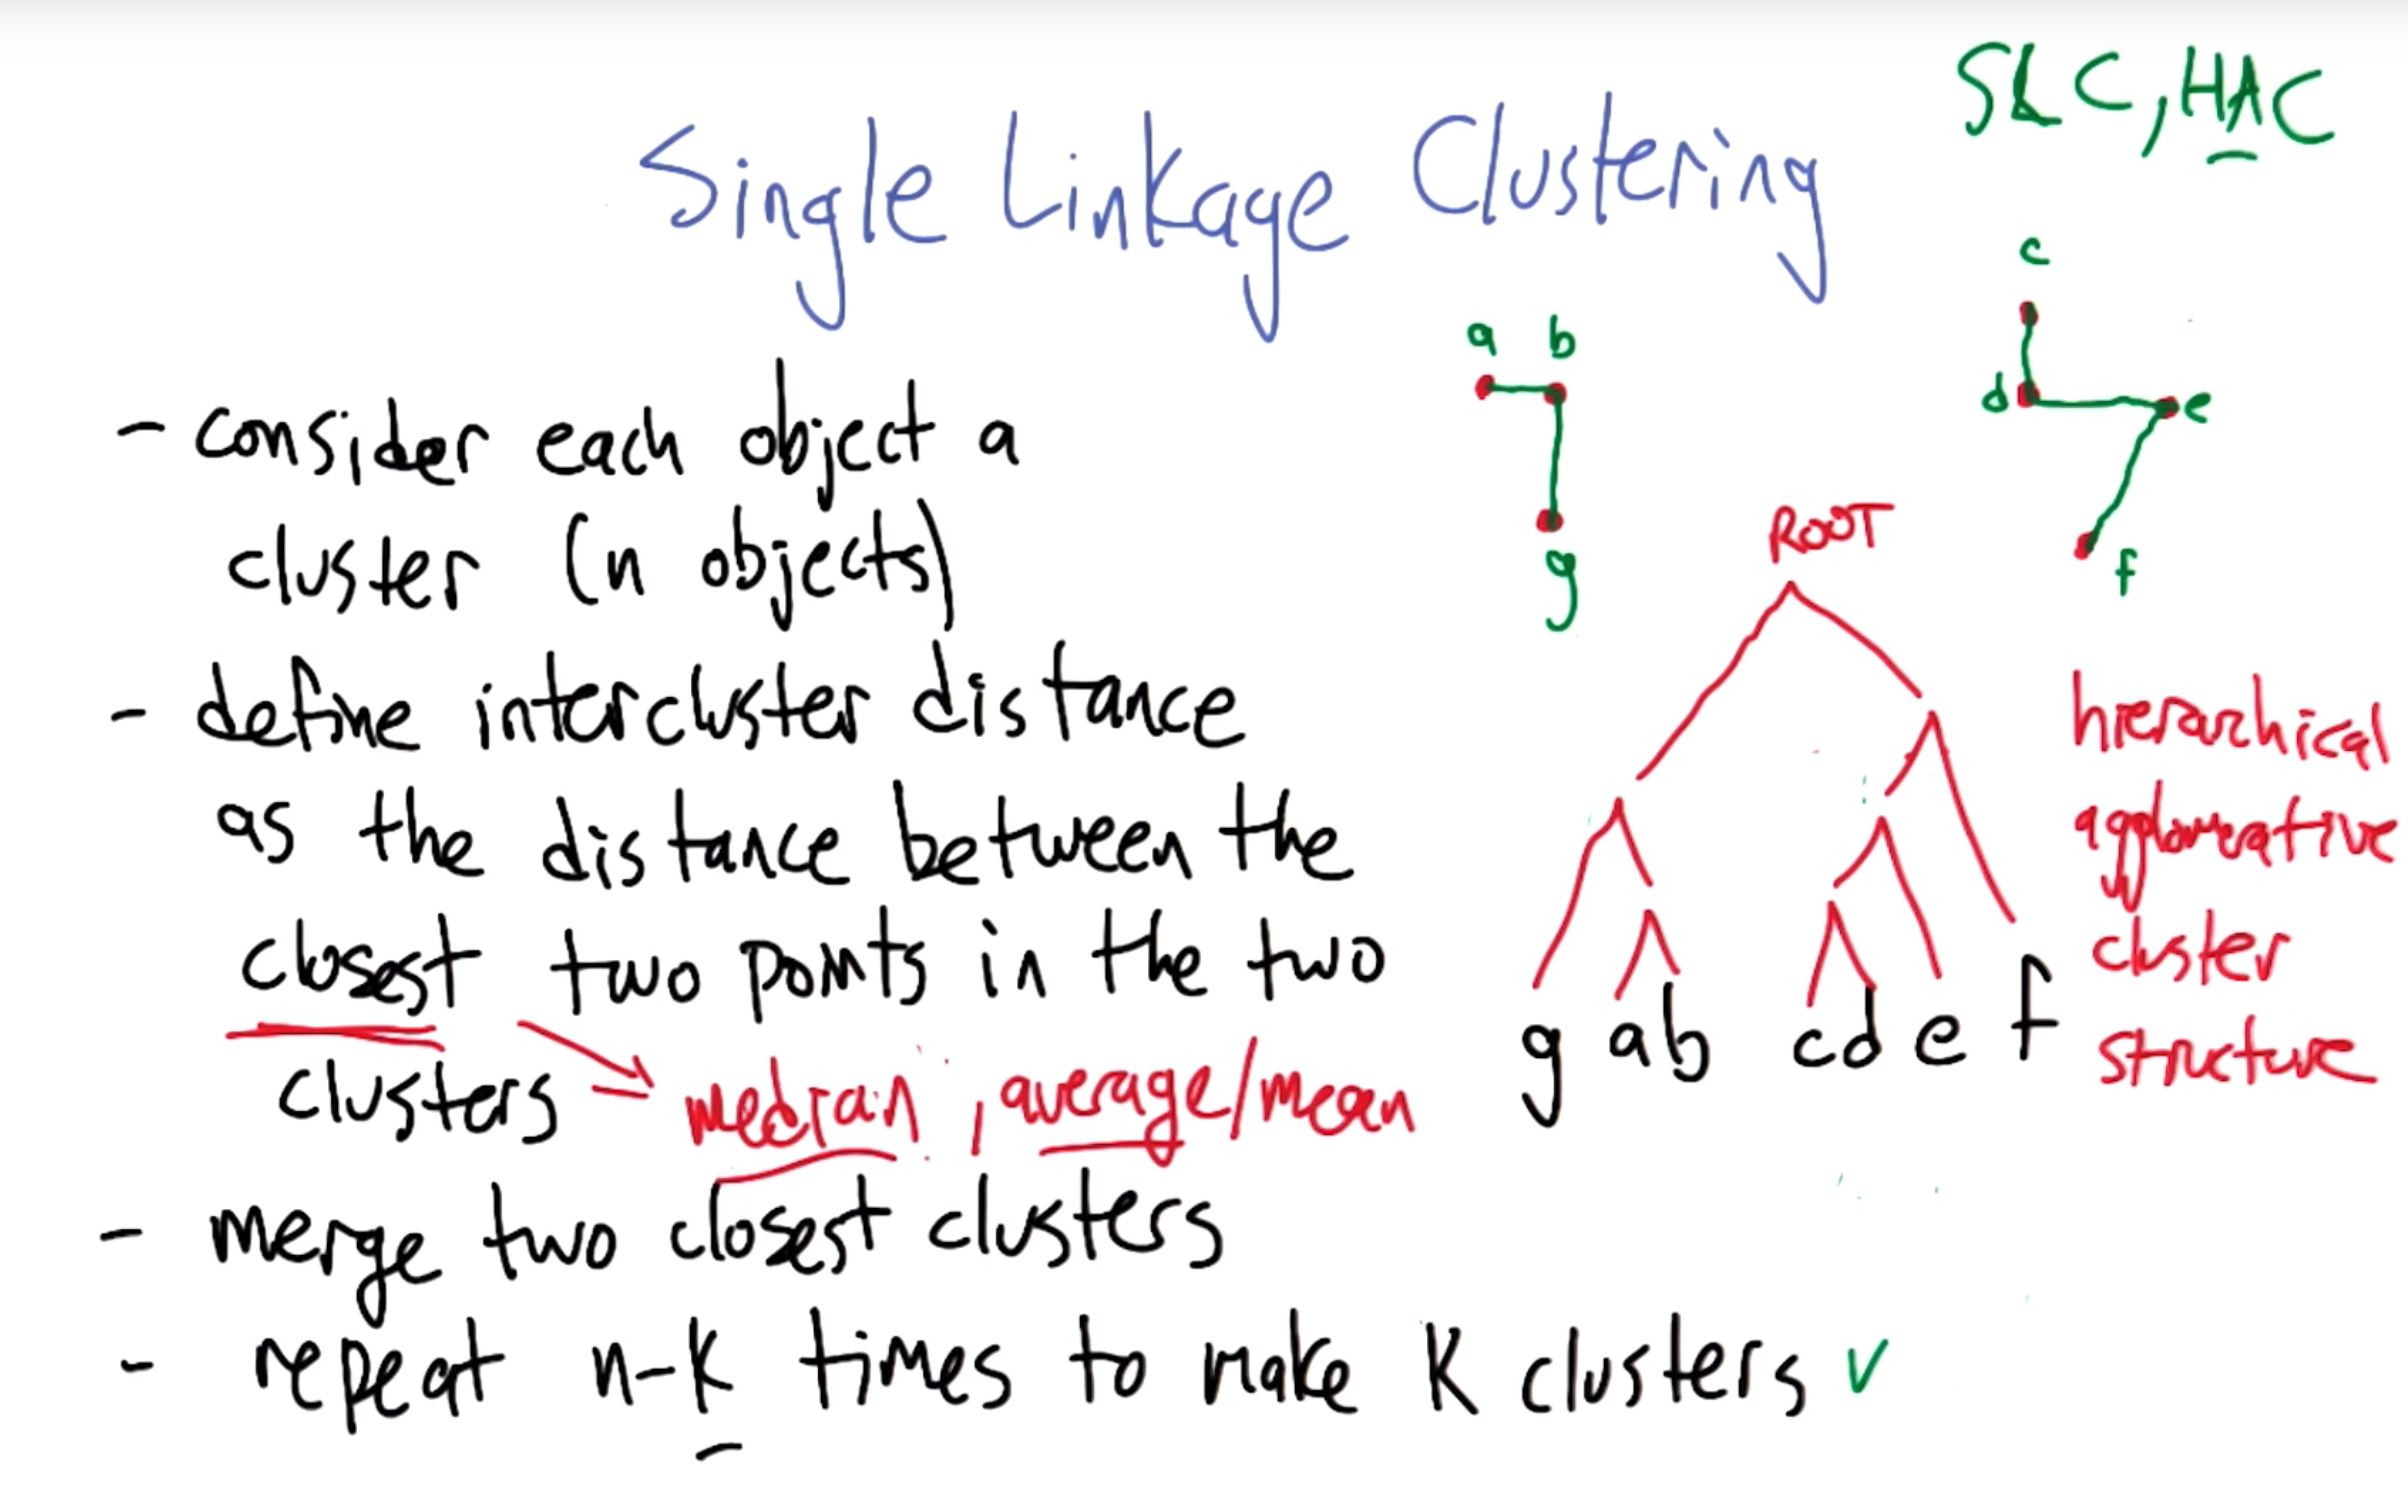
\includegraphics[width=.9\textwidth]{pics/SLC}
	\caption{Single Linkage Clustering} 
	\label{SLC}
\end{figure}
%         --------------------------------------

%%%%%%%%%%%%%%%%%%%%%%%%%%%%%%%%%%%%%%%%%%%%%%%%%%%%%
\subsubsection{K Means Clustering}
K Means Clustering is an \textbf{unsupervised} learning algorithm that will attempt to group similar elements (PCA instead is a factor based rather than clustering algo). Used for market segmentation, cluster customers based on features, identify similar groups, ...

The K Means Algorithm consists of the following steps:
\begin{itemize}
	\item choose a number of clusters “K” (more details later),
	\item randomly assign each point to a cluster, and calculate for each a centroid (or just randomly drop K centroids)
	\item until clusters stop changing, repeat the following loop: (i) for each cluster, compute the cluster centroid by taking the mean vector of points in the cluster and (ii) \textbf{assign} each data point to the cluster for which the centroid is the closest (minimising a distance).
\end{itemize}

%          --------   FIGURE: k_means_algo_loop  -----------
\begin{figure}[htbp] 
	\centering
	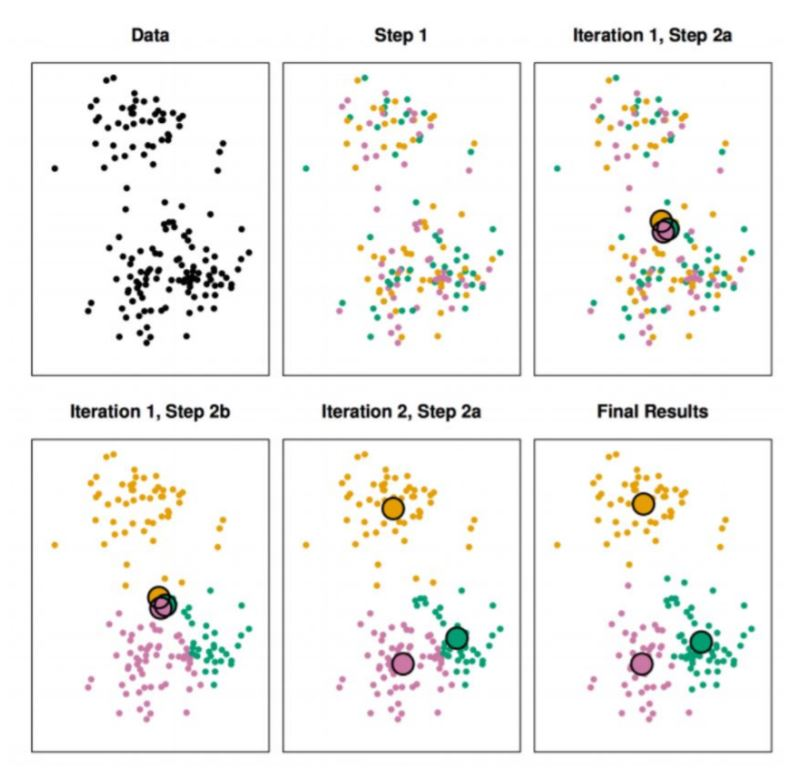
\includegraphics[width=0.6\textwidth]{pics/k_means_algo_loop}
	\caption{K Means algorithm} 
	% \label{k_means_algo}
\end{figure}
%         --------------------------------------
For uniform distributed samples, the centroid initial conditions have a big effect on the final outcome (think of a square of point uniformly distributed and 2 centroids: depending on the latter initial position we may end up splitting the square vertically or horizontally or diagonally, and so). In Sklearn the parameter n\_init (default = 10) in KMeans() may allievate that issue for less degenerate cases (recall: KMeans is a hill-climbing algo, hence initial conditions may be important even for not degenerate case: local minimum - for example in 3 cluster case, two of the centroids start very close and are unable to move so in the end we find only two clusters or, another example, two centroids and the two clusters get divided horizontally across because of bad initial conditions).

There is no easy answer on how to choose the best K. One way is the  elbow method:
\begin{itemize}
	\item compute, for some K values (e.g. 2, 4, 6, 8, etc.), the sum of squared error (SSE) between each cluster member and its centroid,
	\item if you plot K vs. SSE you will see that the error decreases as k gets larger, the idea is to choose he K at which SSE decreases abruptly (this produce an elbow effect n the graph - see following fig) 
\end{itemize} 
%          --------   FIGURE: elbow  -----------
\begin{figure}[htbp] 
	\centering
	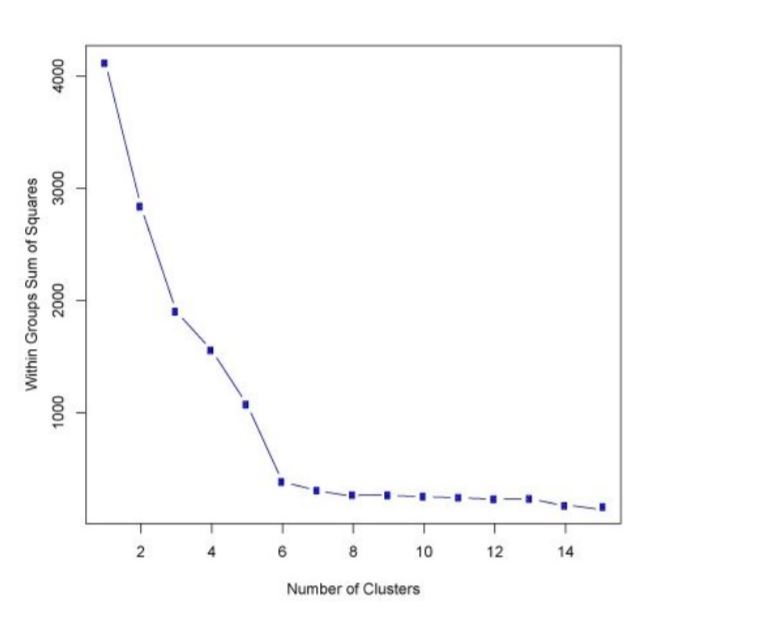
\includegraphics[width=0.6\textwidth]{pics/elbow}
	\caption{Choosing a K value: elbow method} 
	% \label{elbow}
\end{figure}
%         --------------------------------------

\begin{lstlisting}
# 1. get/create data
from sklearn.datasets import make_blobs # arrays
# Create Data
data = make_blobs(n_samples=200, n_features=2, 
centers=4, cluster_std=1.8,random_state=101)

# 2. do some explanatory data analysis
plt.scatter(data[0][:,0],data[0][:,1],c=data[1],cmap='rainbow')
# 'c=' is the color


# 3. K Means Clustering
# create the cluster (NB: no train_test) 
from sklearn.cluster import KMeans
kmeans = KMeans(n_clusters=4) # choose the no. of clusters
kmeans.fit(data[0])

# output
kmeans.cluster_centers_  # coordinates for K's
kmeans.labels_  # the labels, see charts below

# visual output: K mean vs. original (NB: only in our example 
# since we've the labels - not possible since unsupervised)
f, (ax1, ax2) = plt.subplots(1, 2, sharey=True,figsize=(10,6))
ax1.set_title('K Means')  # the chart with the label (NB: 'c=')
ax1.scatter(data[0][:,0],data[0][:,1],c=kmeans.labels_,cmap='rainbow')
ax2.set_title("Original")
ax2.scatter(data[0][:,0],data[0][:,1],c=data[1],cmap='rainbow')
\end{lstlisting}

%%%%%%%%%%%%%%%%%%%%%%%%%%%%%%%%%%%%%%%%%%%%%%%%%%%%%
\subsection{Gaussian Mixture Model}
E.g. Expectation maximization (EM) is a numerical technique for maximum likelihood estimation, and is usually used when closed form expressions for updating the model parameters can be calculated (which will be shown below). \href{http://home.deib.polimi.it/matteucc/Clustering/tutorial_html/mixture.html}{Expectation maximization} is an iterative algorithm and has the convenient property that the maximum likelihood of the data strictly increases with each subsequent iteration, meaning it is guaranteed to approach a local maximum or saddle point \\
Gaussian Mixture Model ('GMM') is a soft/probabilistic clustering algorithm, which means that - contrary to K-Means where every datapoint must belong to a cluster - GMM assigns a probability to a point belonging to a specific cluster and revising such probability at each iteration. In other words, GMM is a generalisation of KM that incorporates the data covariance structure and centers of latent Gaussians. More on \href{http://scikit-learn.org/stable/modules/mixture.html#expectation-maximization}{sklearn on GMM}.

\begin{lstlisting}
from sklearn.mixture import GaussianMixture
from sklearn.metrics import silhouette_score
num_clusters = [i for i in range(2, 10)] + [20, 50] 

for _n in num_clusters:
	clusterer = GaussianMixture(n_components=_n).fit(reduced_data)
	preds = clusterer.predict(reduced_data)
	# # before we ran
	# pca = PCA(n_components=2).fit(good_data)
	# reduced_data = pca.transform(good_data)
	centers = clusterer.means_
	score = silhouette_score(reduced_data, preds)
	print("{} clusters has a {} score silhouette" .format(_n, score)) 
\end{lstlisting}
Silhouette analysis can be used to check how \textit{balanced} are the clusters obtained from different values of number of clusters. Remark that in certain cases, you can even choose a value for number of clusters which gives a sub-optimal score. For example, in this \href{http://scikit-learn.org/stable/auto_examples/cluster/plot_kmeans_silhouette_analysis.html#sphx-glr-auto-examples-cluster-plot-kmeans-silhouette-analysis-py}{link}, 2 is not considered optimal, despite having a better Silhouette score, because it doesn't result in balanced clusters, while 4 does.
 
Since the data ($reduced_data$) is currently reduced in dimension ($pca.transform()$) and scaled by a logarithm, we can recover the representative customer spending from these data points by applying the inverse transformations.	
\begin{lstlisting}
# Inverse transform the centers
log_centers = pca.inverse_transform(centers)

# Exponentiate the centers
true_centers = np.exp(log_centers)

segments = ['Segment {}'.format(i) for i in range(0,len(centers))]
true_centers = pd.DataFrame(np.round(true_centers), columns = data.keys())
true_centers.index = segments
\end{lstlisting}
	
%%%%%%%%%%%%%%%%%%%%%%%%%%%%%%%%%%%%%%%%%%%%%%%%%%%%%
\subsection{DBSCAN}
Its parameters are (i) the distance (epsilon) and (ii) min number of points to get a cluster (vs. num. of clusters for K-means). In short, DBSCAN selects a data point and check if within its specified distance there are a min number of points (e.g. 5), if so it defines a cluster (and check again for each point inside and individuate 'border' points of the cluster); if a selected point does not contain the 5 points in the distance neighbour is defined as a 'noise point'. 

See visual comparison in fig. \ref{_dbscan}.

%          --------   FIGURE: DBSCAN  -----------
\begin{figure}[htbp] 
	\centering
	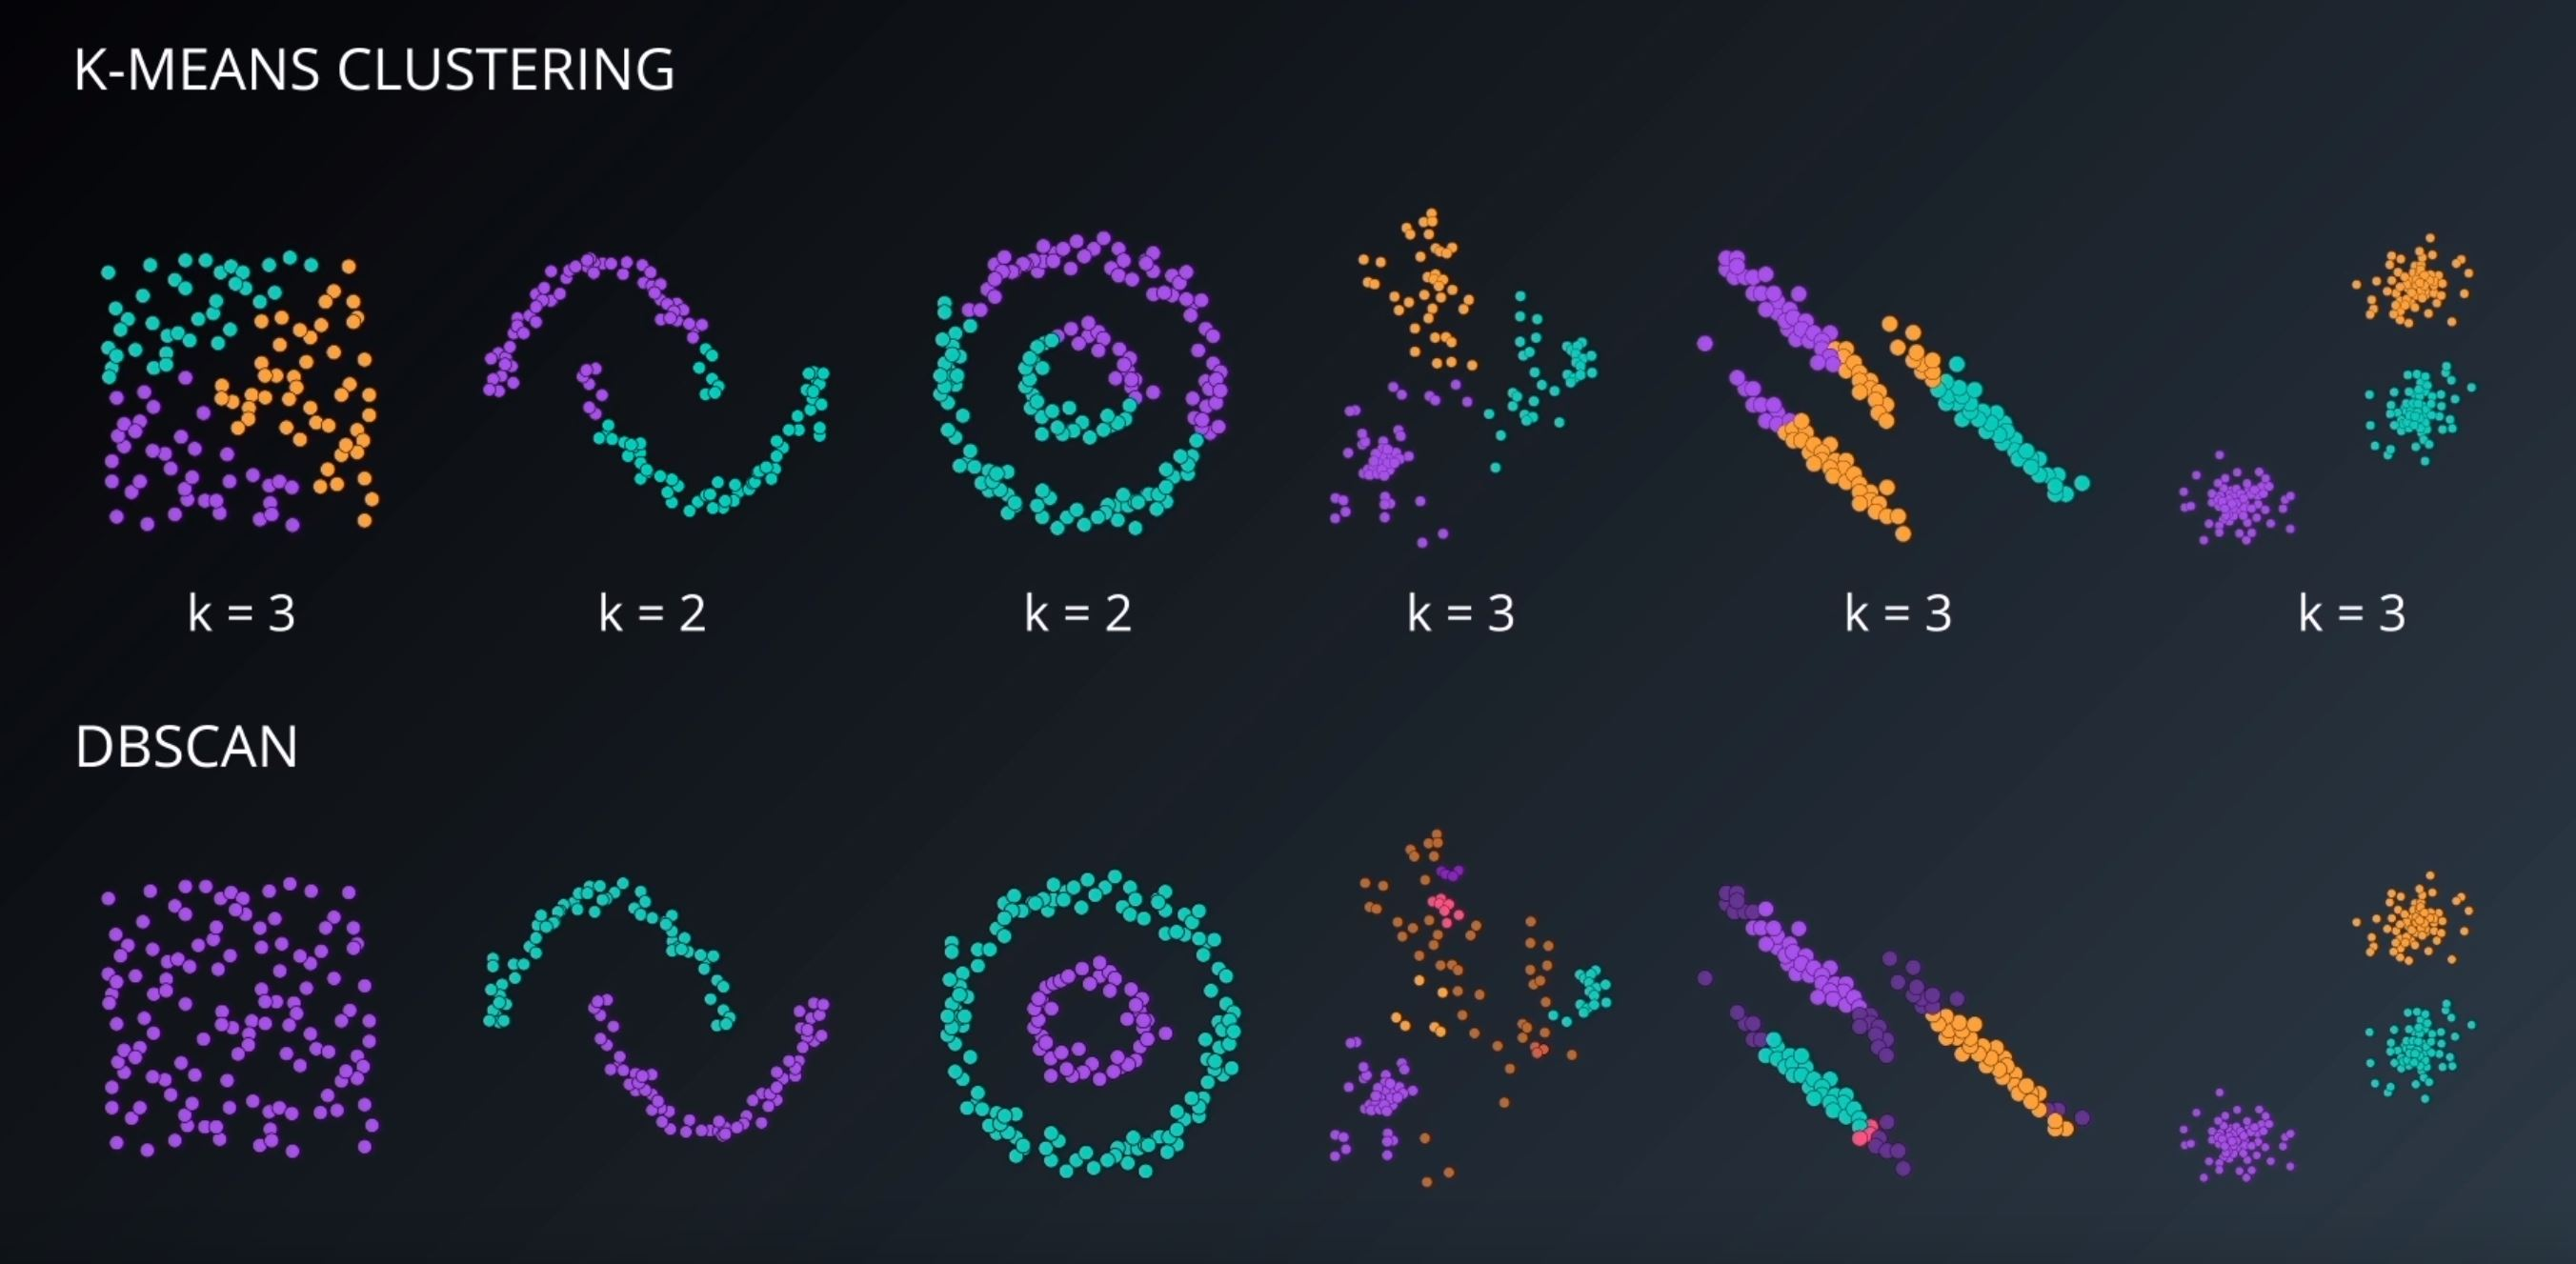
\includegraphics[width=0.7\textwidth]{pics/dbscan}
	\caption{Density-based Clustering vs. K-means} 
	\label{_dbscan}
\end{figure}
%         --------------------------------------

\begin{lstlisting}
# 1. get/create data
from sklearn.datasets import load_iris
# Create Data
data = load_iris().data

# create the cluster
from sklearn.cluster import DBSCAN
db_scan = DBSCAN(eps=0.5, min_samples=5) # 2 params
db_scan.fit(data)

db_scan.labels_  # the labels (-1: noise)
\end{lstlisting}

%%%%%%%%%%%%%%%%%%%%%%%%%%%%%%%%%%%%%%%%%%%%%%%%%%%%%%
%	REINFORCEMENT LEARNING
%%%%%%%%%%%%%%%%%%%%%%%%%%%%%%%%%%%%%%%%%%%%%%%%%%%%%%
\section{Reinforcement Learning}	\label{reinforcement_learning}

%%%%%%%%%%%%%%%%%%%%%%%%%%%%%%%%%%%%%%%%%%%%%%%%%%%%%%
\subsection{Markov decision processes (MDP)} \label{mdp}
Let us introduce the framework:
\begin{itemize}
	\item \textbf{states}: $S$, set of states we can be in (e.g. all coordinates in a matrix);
	\item \textbf{actions}: $A(s)$, $A$ e.g. moves in a matrix (up, down, left or right);
	\item \textbf{model}: $T(s,a,s') \sim Pr(s'|s,a)$, transition model that is a function of a state, action and another state (which can be the same), in other words it describes the rules of the game. Note that transitions (probabilities) are \underline{Markovian} - ie. they depend on present state only (for tractability) - and process is \underline{stationary}, i.e. rules do not change
	\item \textbf{reward}: $R(s)$ (or $R(s,a)$ or $R(s,a,s')$), reward that you get from entering into a state (whether positive, negative or null).
\end{itemize}
Any solution of the above stated problem is called a \textbf{policy}: a function that takes a (particular) state and returns an action $\pi(s) \rightarrow a$;  and the \textit{optimal} policy is the one that optimise the long-term reward. So for each state we have an (local) action and possible a reward - which is different from a \textit{plan}, that is a series of actions to take to reach the goal.  

Rewards can be also \textit{delayed} , i.e. they can materialise after a few actions and not for each incremental action. E.g. when you play chess, you see the reward of a poor move only later (and you may not know where such a poor move occurred) - this is called \textit{temporal credit assignment}. And this temporal sequence is an important difference between reinforcement and supervised learning.

In addition, \textit{reward values} do matter. E.g. notice that in order to avoid the negative absorbing state in the left-hand side of fig. \ref{reinforcement_1} the optimal policy (for the two central bottom states) is to take the long way around - which is not the case if there was no uncertainty or if the reward was different. The right-side in the same fig. shows indeed that for different rewards (here two extreme cases) the optimal policy is quite different - the point is that in choosing rewards domain-knowledge is paramount.
%          --------   FIGURE: reinforcement 1  -----------
\begin{figure}[htbp] 
	\centering
	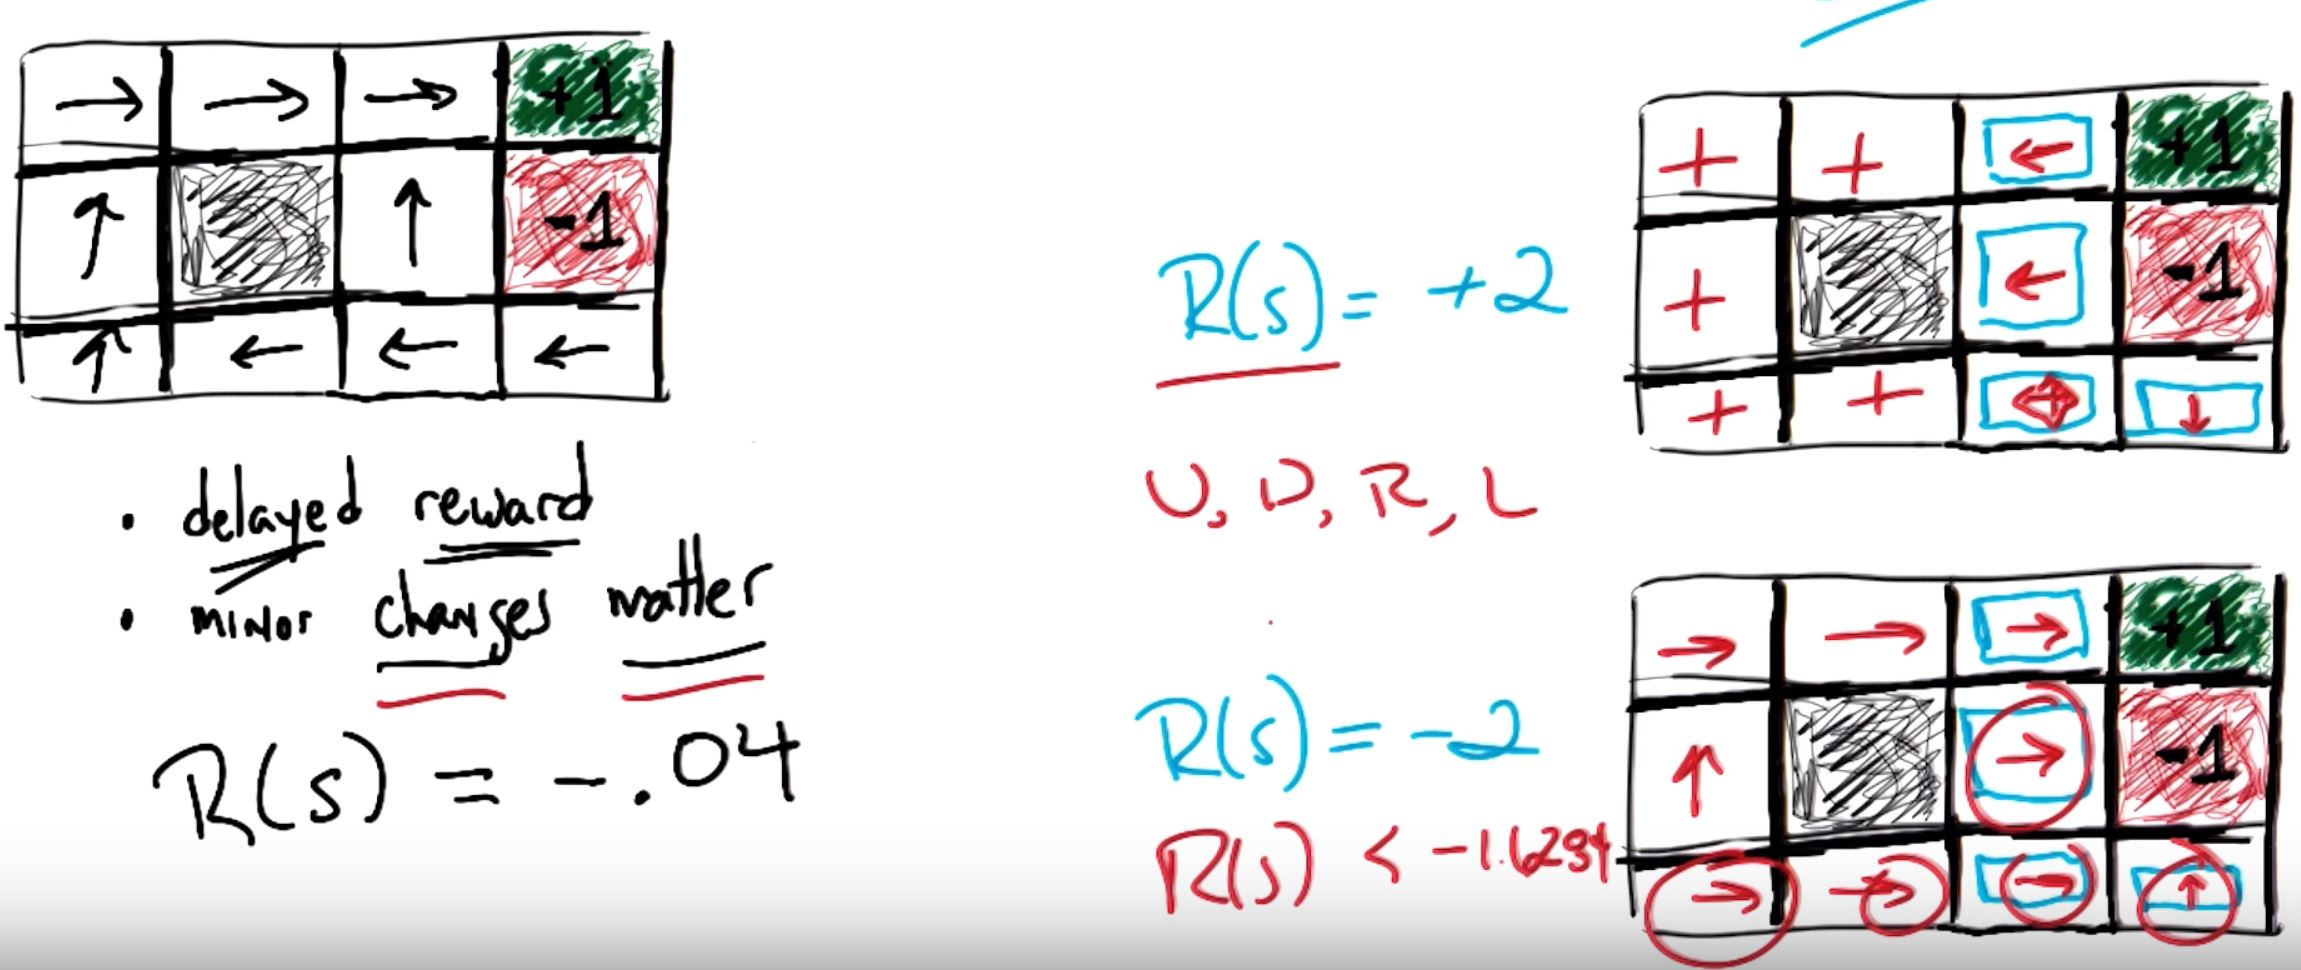
\includegraphics[width=0.9\textwidth]{pics/reinforcement_1}
	\caption{Simple game} 
	\label{reinforcement_1}
\end{figure}
%         --------------------------------------

Note also assumptions made so far: (i) \textbf{infinite horizons} - policy in the left-hand side of fig. \ref{reinforcement_1} assumes no time limit, but with fewer steps left we may need to take more risk (and this may even give two different actions for same state, depending on time-left so far i.e. $\pi(s, time) \rightarrow a$) - and (ii) \textbf{stationary preferences} or, in other words, we are assuming a type of utility where we  sum the sequence of rewards, i.e. if $U(s_0,s_1, s_2, \ldots ) > U(s_0,s'_1, s'_2, \ldots)$ then $U(s_1, s_2, \ldots) > U(s'_1, s'_2, \ldots)$. In particular, the function to use is the \textbf{discounted reward}:
\[	U(s_0,s_1, s_2, \ldots ) = \sum_{t=0}^{\infty} \gamma^t R(s_t)
\]
since the trailing-off introduced by $\gamma^t$, where $\gamma$ in $[0, 1)$,  makes the sum bounded from the above - indeed $U(\ldots )\eqslantless \sum_{t=0}^{\infty} \gamma^t R_{max} = R_{max} / (1-\gamma)$ - which is useful for infinite horizons by avoiding that the reward explodes to infinity (also intuitive: a reward now is worth more than tomorrow).

Now we can write the optimal policy (i.e. the one optimising the long-term reward):
\[ \pi^* = \text{argmax}_\pi \; E \big(\sum_{t=0}^{\infty} \gamma^t R(s_t) \; |\; \pi \big)
\]
and if we follow such policy the Utility to be in a given state $s$ is:
\[ U^{\pi}(s) = E \big(\sum_{t=0}^{\infty} \gamma^t R(s_t) \; |\; \pi, s=s_0 \big)  
\]
which is not equal to the reward $R(s)$ - the difference is that the latter is the \textit{immediate} reward, whilst the utility also incorporates the \textit{expected future} rewards to be in such state $s$ now (e.g. if you got to college, you spend 10k and receives an immediate negative rewards, but your utility may still be positive... in short, you can take some very negative immediate rewards now for future bigger rewards), which means that
\[ \pi^*(s) = \text{argmax}_a \; \sum_{s'} \; T(s, a, s') \; U^{\pi^*}(s)
\]
and finally we get the \textbf{Bellman equation} - reward of the current state plus a discount of all future ones: 
\[   U(s) = R(s) + \gamma \; max_a \; \sum_{s'} \; T(s, a, s') \; U^{\pi^*}(s)
\]
which can be seen as a \textit{recursive} equation (see 2nd top equation in fig. \ref{bellman_quiz}) with all ingredients in one place.
%          --------   FIGURE: bellman quiz  -----------
\begin{figure}[htbp] 
	\centering
	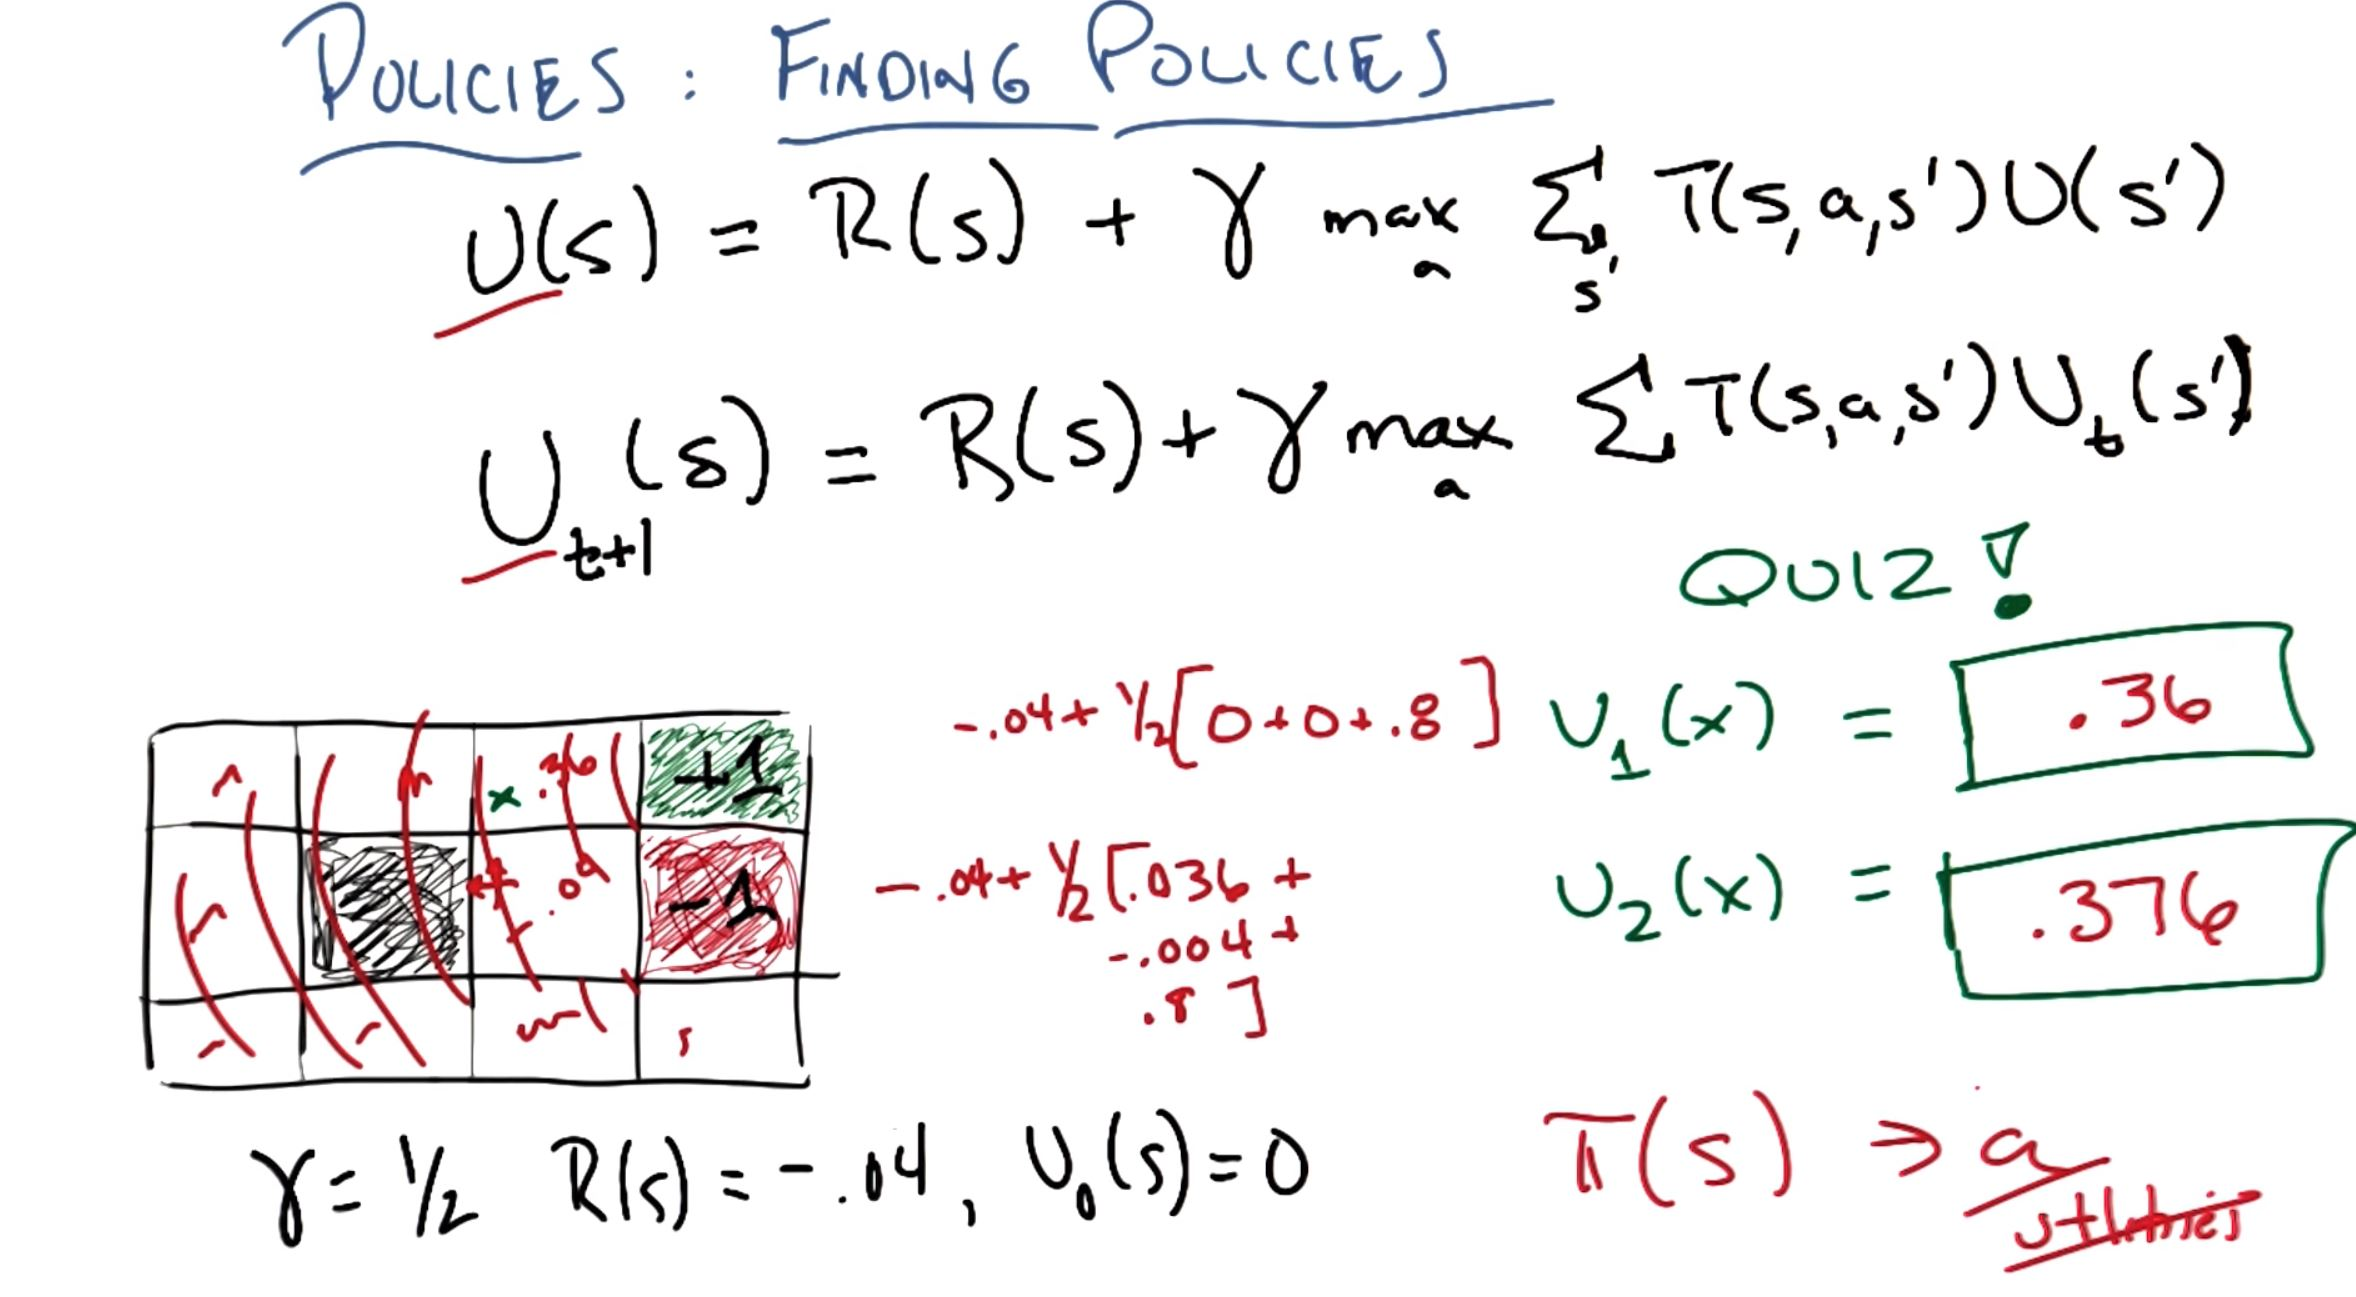
\includegraphics[width=0.7\textwidth]{pics/bellman_quiz}
	\caption{Bellman equation - quiz} 
	\label{bellman_quiz}
\end{figure}
%         --------------------------------------

Suppose that there are $n$ possible states, then the Bellman equation is really a set of $n$ equations in $n$ unknowns, but the $max$ function makes it non-linear (so not possible to solve it as usual by matrix inversion) - but we can use the following simple algorithm (called \textbf{value iteration}): (i) start with some arbitrary utility values, (ii) update utilities (for all $n$ equations, i.e. states) based on neighbours, and (iii) repeat. Intuitively, the reason such an algo works for arbitrary utilities values is that $R(s)$ are correct and the algo simply propagates such information back and forth; see fig. \ref{bellman_solution} for a sketch of the proof that value iteration does converge. A little quiz to add intuition is in fig. \ref{bellman_quiz}.
%          --------   FIGURE: bellman solution  -----------
\begin{figure}[htbp] 
	\centering
	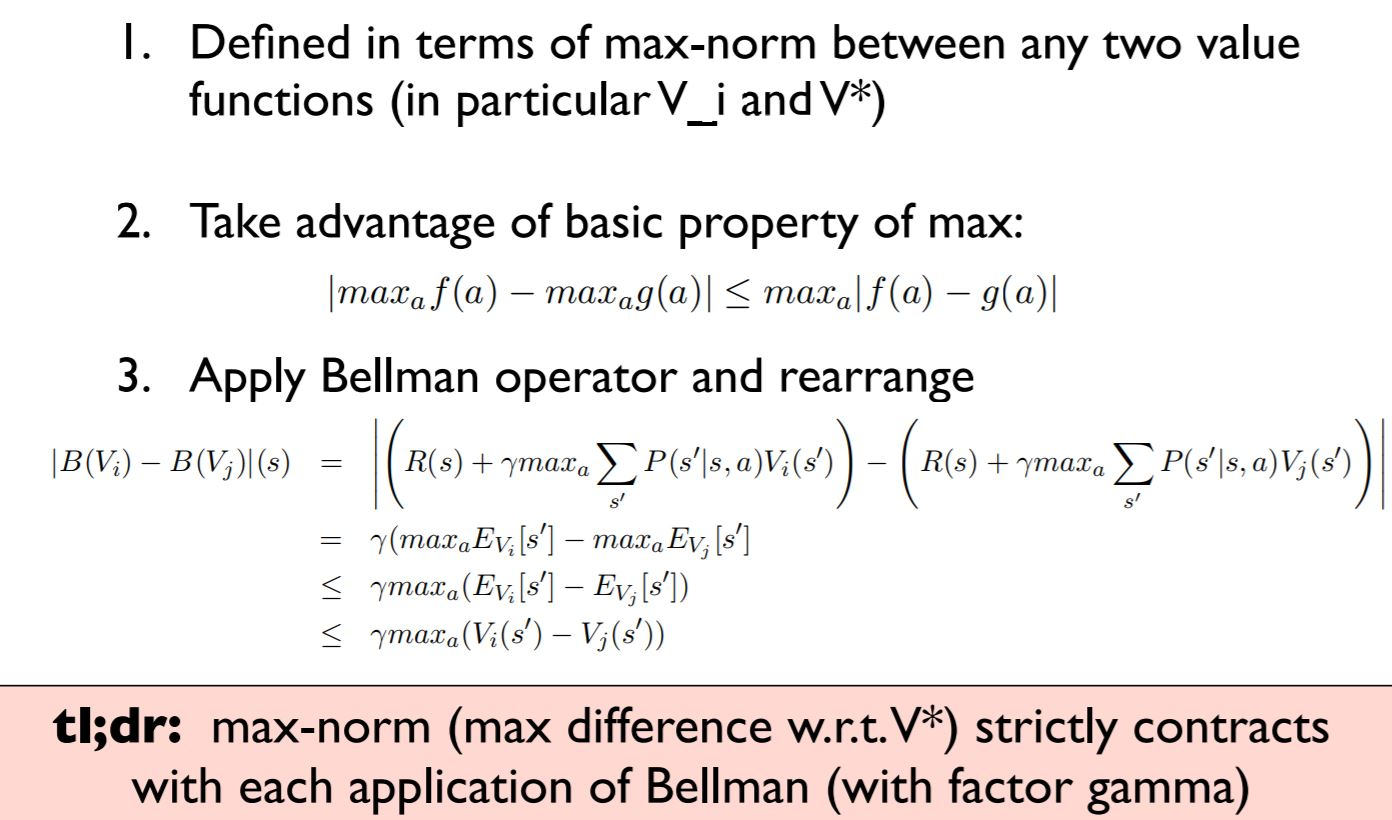
\includegraphics[width=0.75\textwidth]{pics/bellman_solution}
	\caption{Bellman equation - proof sketch} 
	\label{bellman_solution}
\end{figure}
%         --------------------------------------

Since we really care about policies, rather than calculating utilities - we can re-express the bellman equation as in fig. \ref{finding_policies}. Note that the contemporaneous $t$ on both $U$ and that expressing it as a function of policies removes the max function making easier the solution. This algo is called \textbf{policy iteration}.
%          --------   FIGURE: finding policies  -----------
\begin{figure}[htbp] 
	\centering
	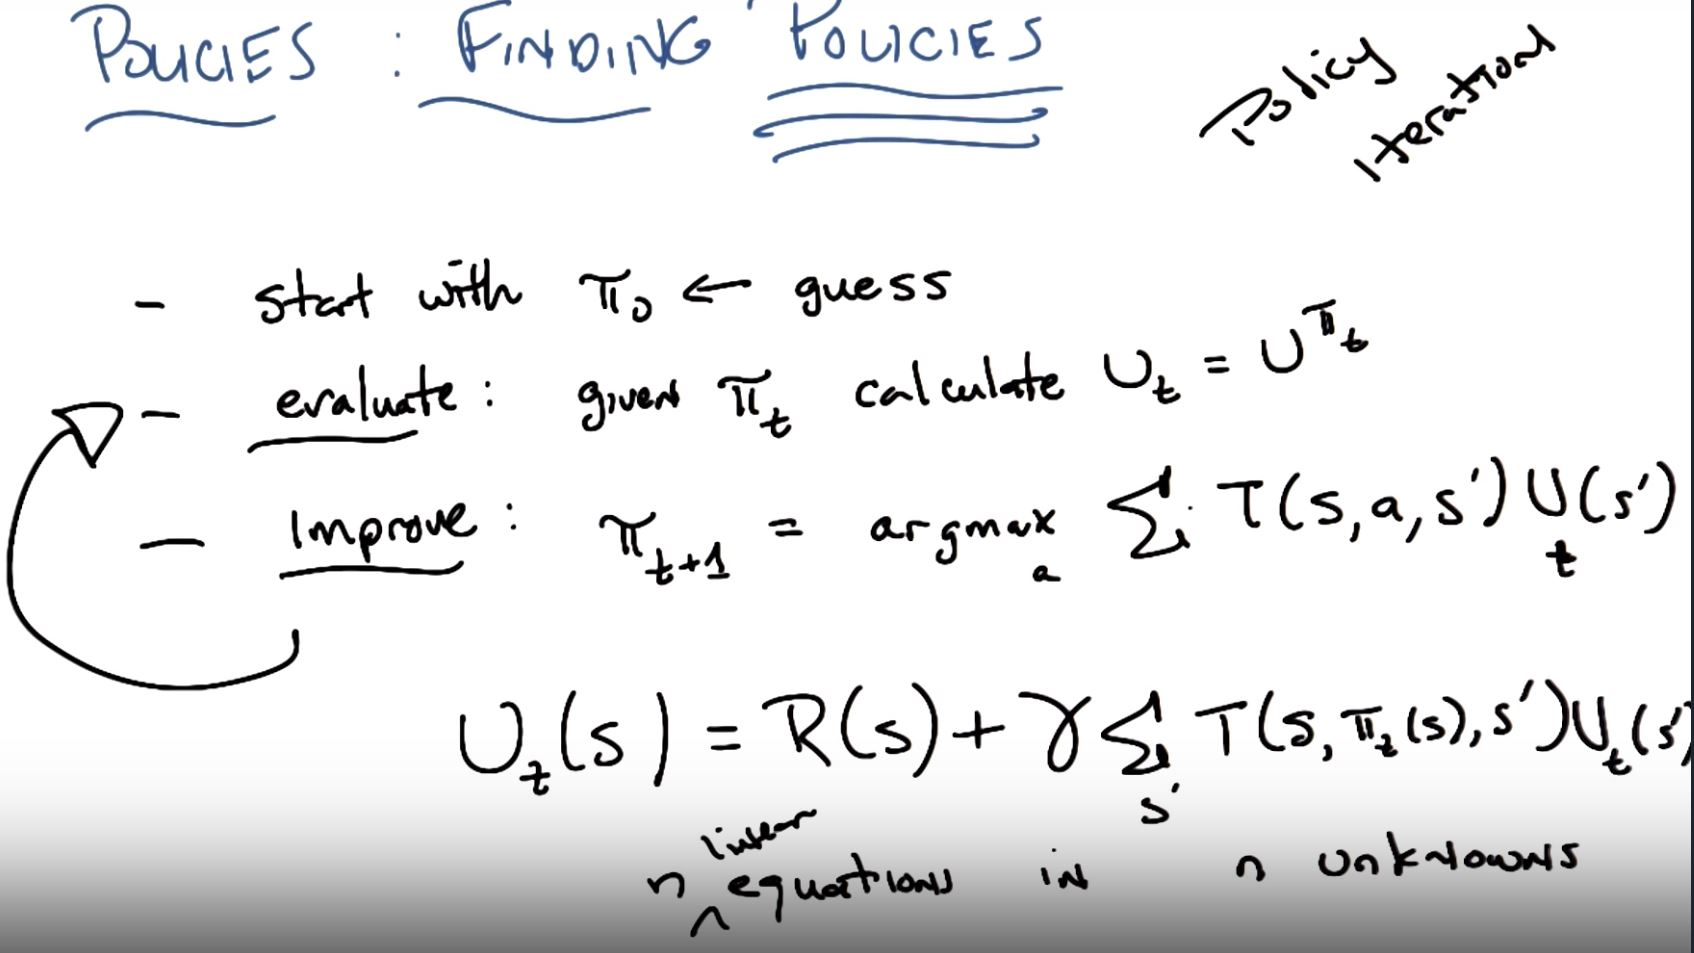
\includegraphics[width=0.7\textwidth]{pics/finding_policies}
	\caption{Policy iteration} 
	\label{finding_policies}
\end{figure}
%         --------------------------------------

%%%%%%%%%%%%%%%%%%%%%%%%%%%%%%%%%%%%%%%%%%%%%%%%%%%%%%
\subsection{Reinforcement learning in MDP}
RL 'APIs': \\
\begin{itemize}
	\item Planning: \\model (transitions and rewards) $\rightarrow$ PLANNER $\rightarrow$ policy 
	\item Reinforcement Learning: \\ transitions ($s, a, r, s'$) $\rightarrow$ LEARNER $\rightarrow$ policy
	\item transitions   $\rightarrow$ MODELLER $\rightarrow$ model
	\item model $\rightarrow$ SIMULATOR $\rightarrow$ transitions
\end{itemize}

In the Reinforcement Learning, instead of \textit{computing} a policy as in Planning, we \textit{learn} it. The last two are sub-components (opposite of each other).

Why 'reinforcement'? think of a lab mouse that sees a stimulus, takes an action and get a reward that strengthens the response to such a stimulus. In short reinforcement means 'reward maximisation', also in psychology.


Note that PLANNER are either (i) valuation or (ii) policy iteration algorithms. Two different ways to build RL - see fig. \ref{RL_approaches}.
%          --------   FIGURE: RL approaches  -----------
\begin{figure}[htbp] 
	\centering
	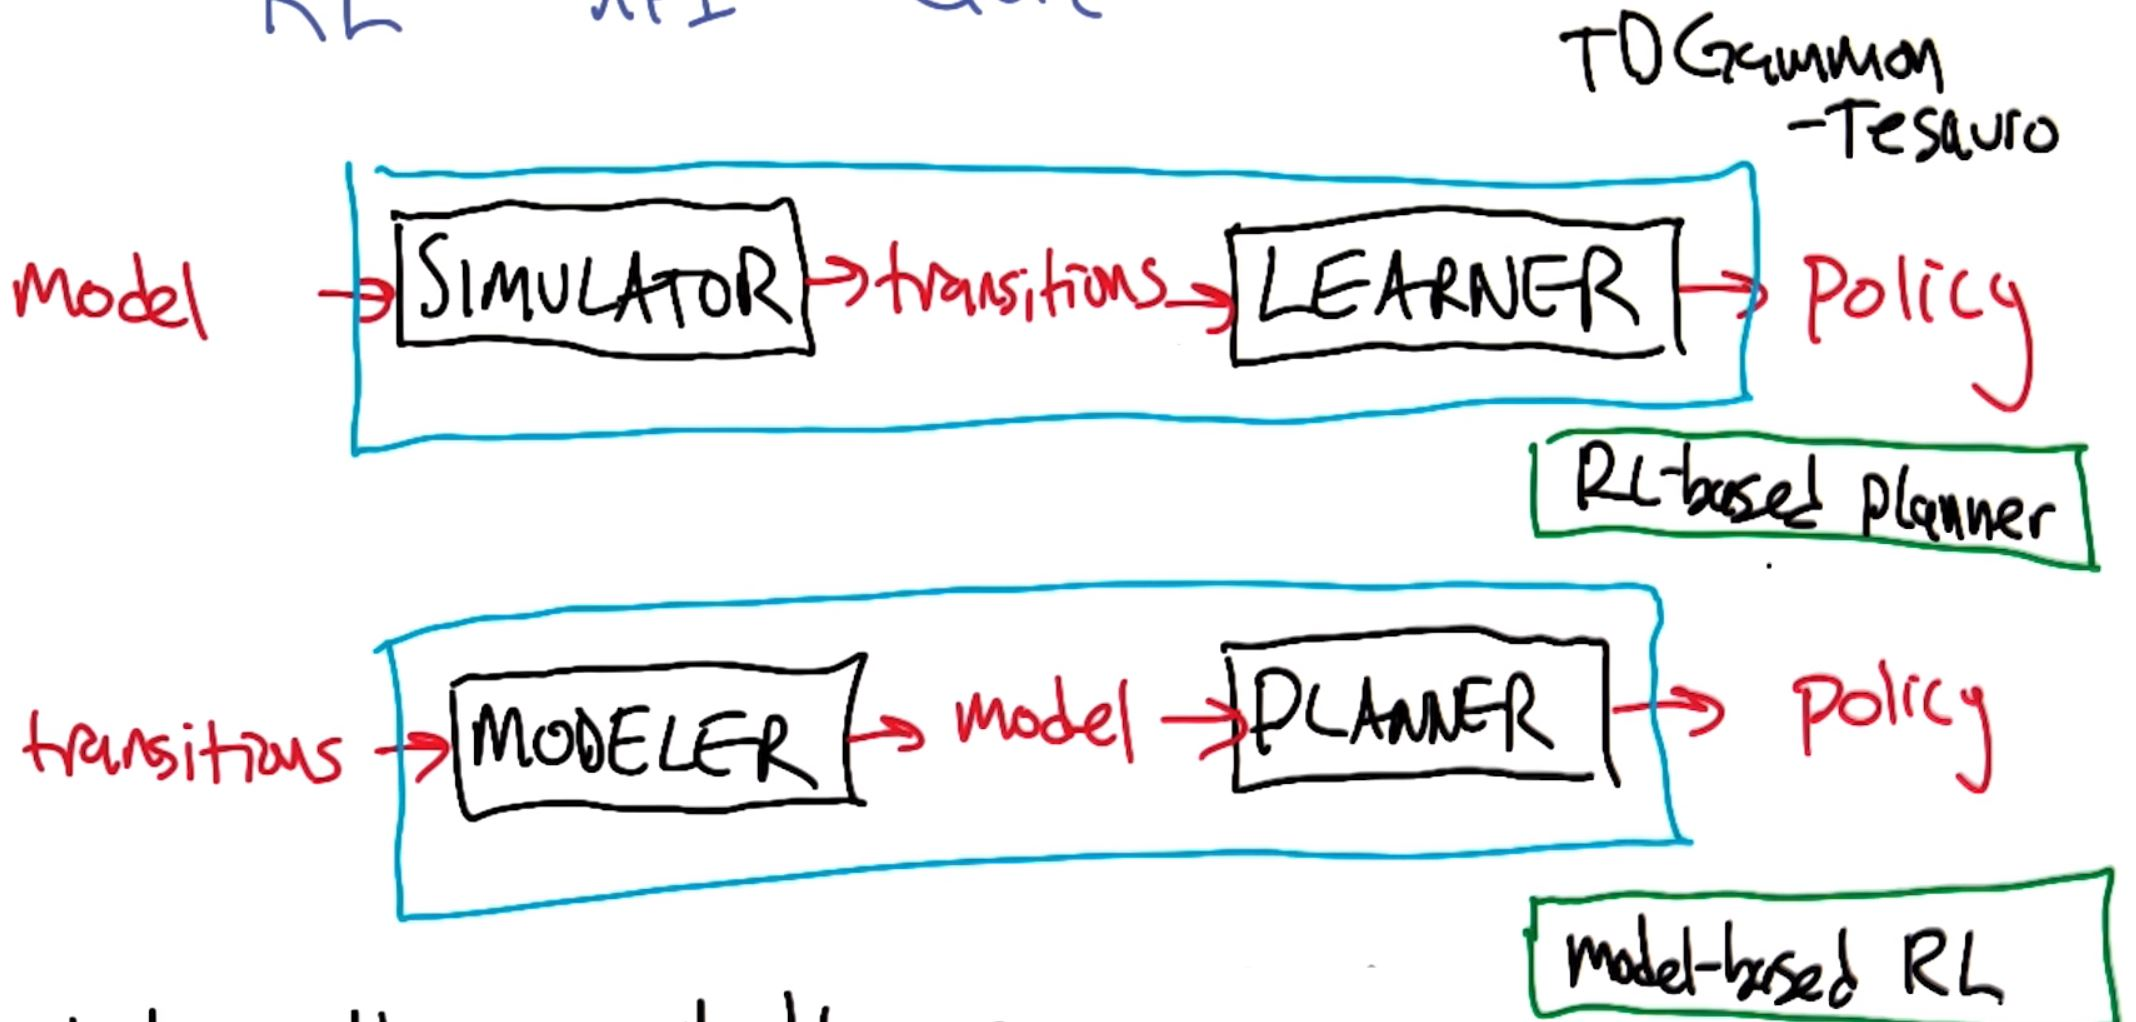
\includegraphics[width=0.7\textwidth]{pics/RL_approaches}
	\caption{RL-based planner and model-based RL} 
	\label{RL_approaches}
\end{figure}
%         --------------------------------------

There are three ways to solve a RL problem, the one in the middle of fig. \ref{3_approaches_to_RL} is the one most pursued in practice since in a goldilocks spot between direct and indirect learning. 
%          --------   FIGURE: 3 RL approaches  -----------
\begin{figure}[htbp] 
	\centering
	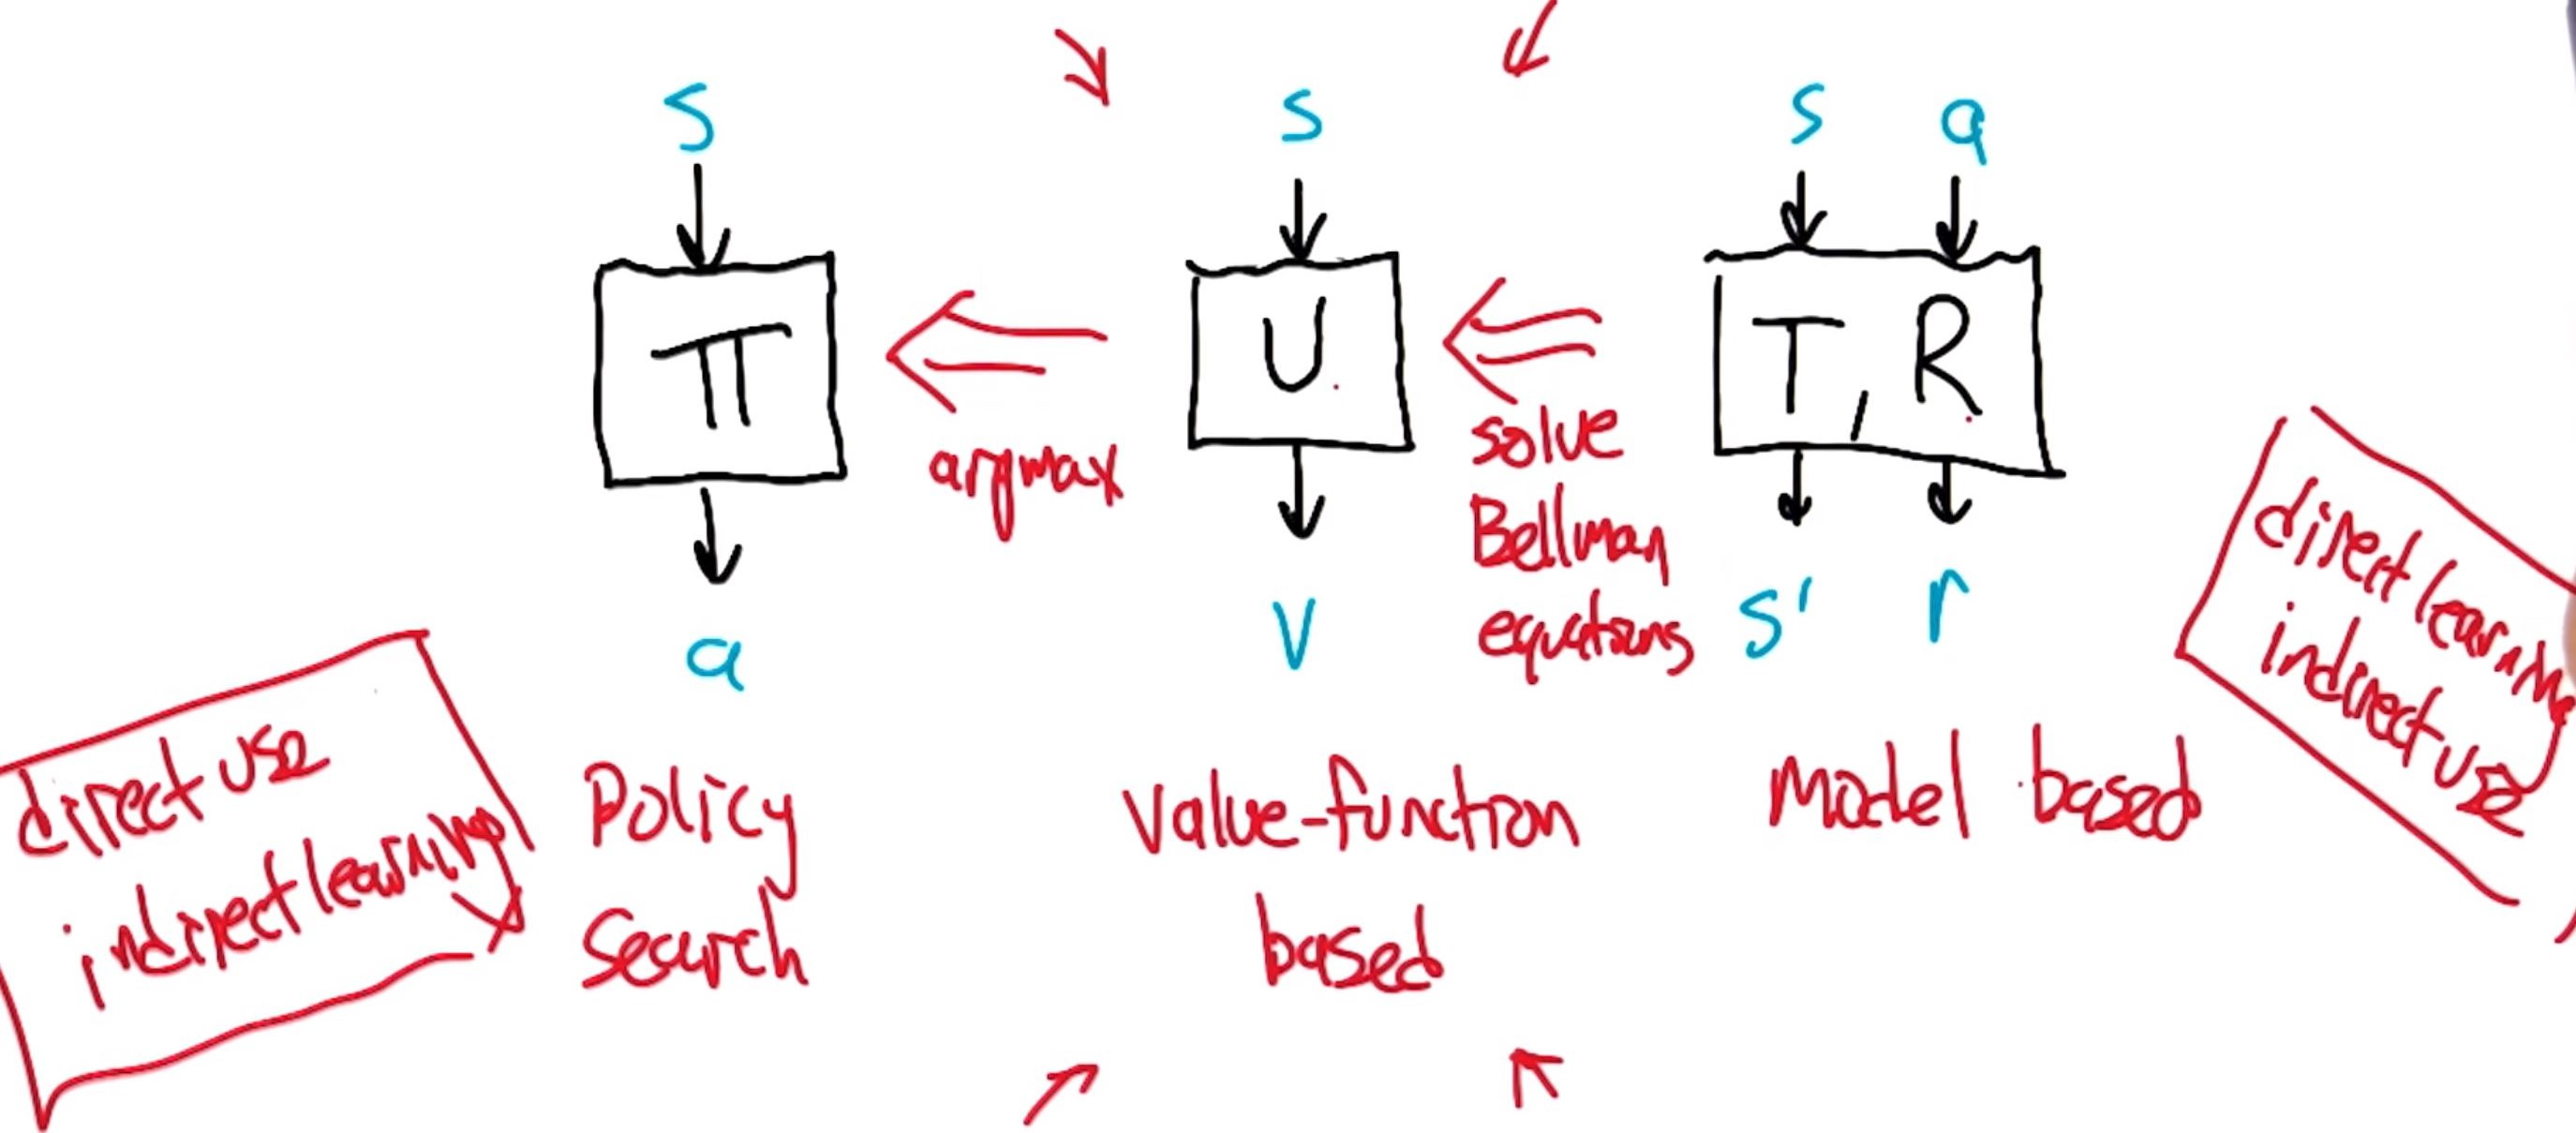
\includegraphics[width=0.7\textwidth]{pics/3_approaches_to_RL}
	\caption{Three approaches to RL} 
	\label{3_approaches_to_RL}
\end{figure}
%         --------------------------------------

By defining a new kind of value function $Q$ in fig \ref{q_learning} (which gets elements from $U(s)$ and $\pi(s)$ seen earlier) then the optimisation problem (finding optimal policy) is easier: we are forcing the algo to learn via actions.
%          --------   FIGURE: 3 RL approaches  -----------
\begin{figure}[htbp] 
	\centering
	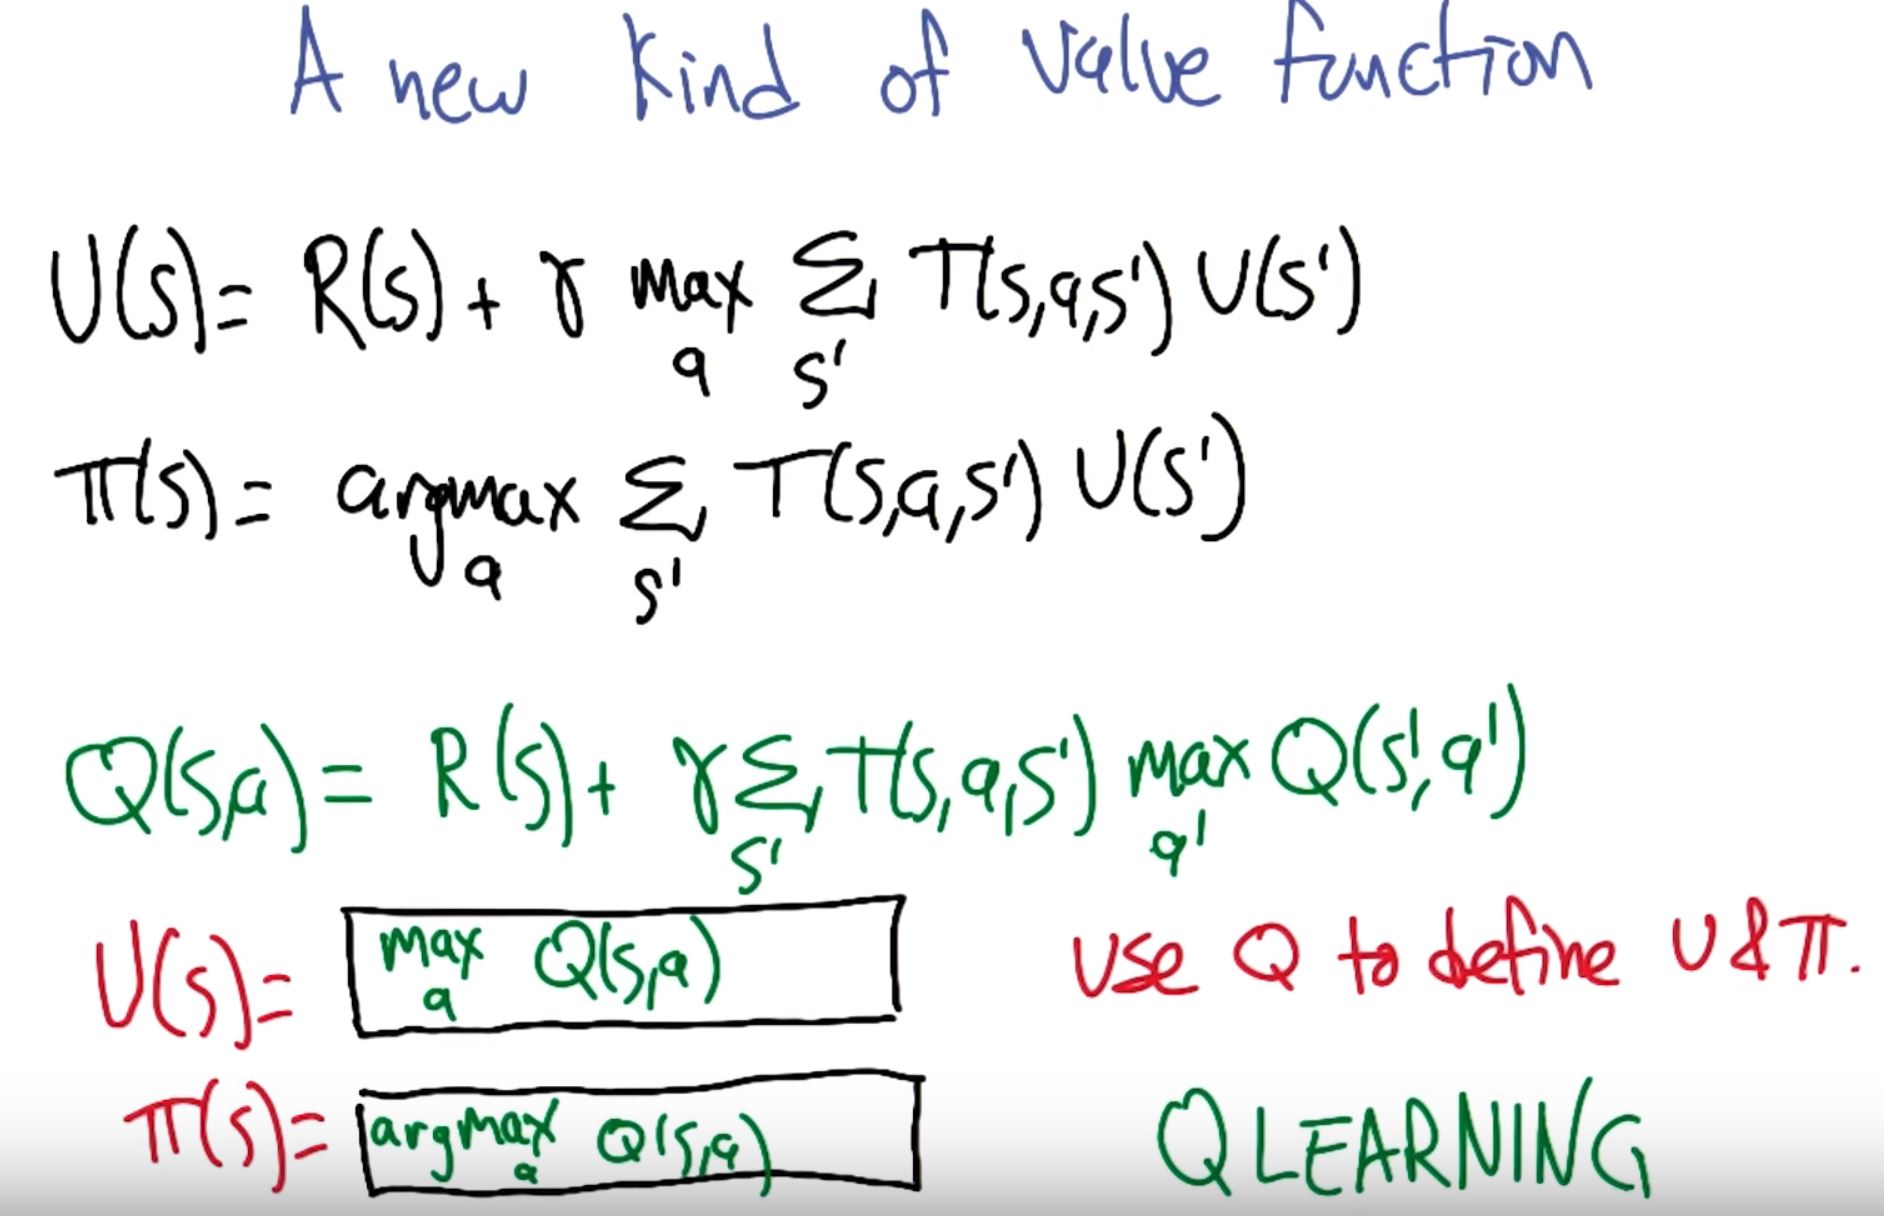
\includegraphics[width=0.42\textwidth]{pics/q_learning}
	\caption{Q-Learnig} 
	\label{q_learning}
\end{figure}
%         --------------------------------------

We are left with estimating Q from transitions. From transition (we observe a state, an action is chosen, we get a reward and land in a state) - from state and action, we move by a learning rate $\alpha$ (which can be time independent) in the direction of the immediate reward and the discounted estimated value of the next step (fig. \ref{estimating_Q} - NB: Q-learning is a family\footnote{Family because Q-learning algos can be different depending on (i) how to initialise Q, (ii) how decay $\alpha_t$ and (iii) how to choose actions.} of \textit{model-free} reinforcement learning algorithms), incrementally (similar like repeating sampling  and computing the average):
%          --------   FIGURE: 3 RL approaches  -----------
\begin{figure}[htbp] 
	\centering
	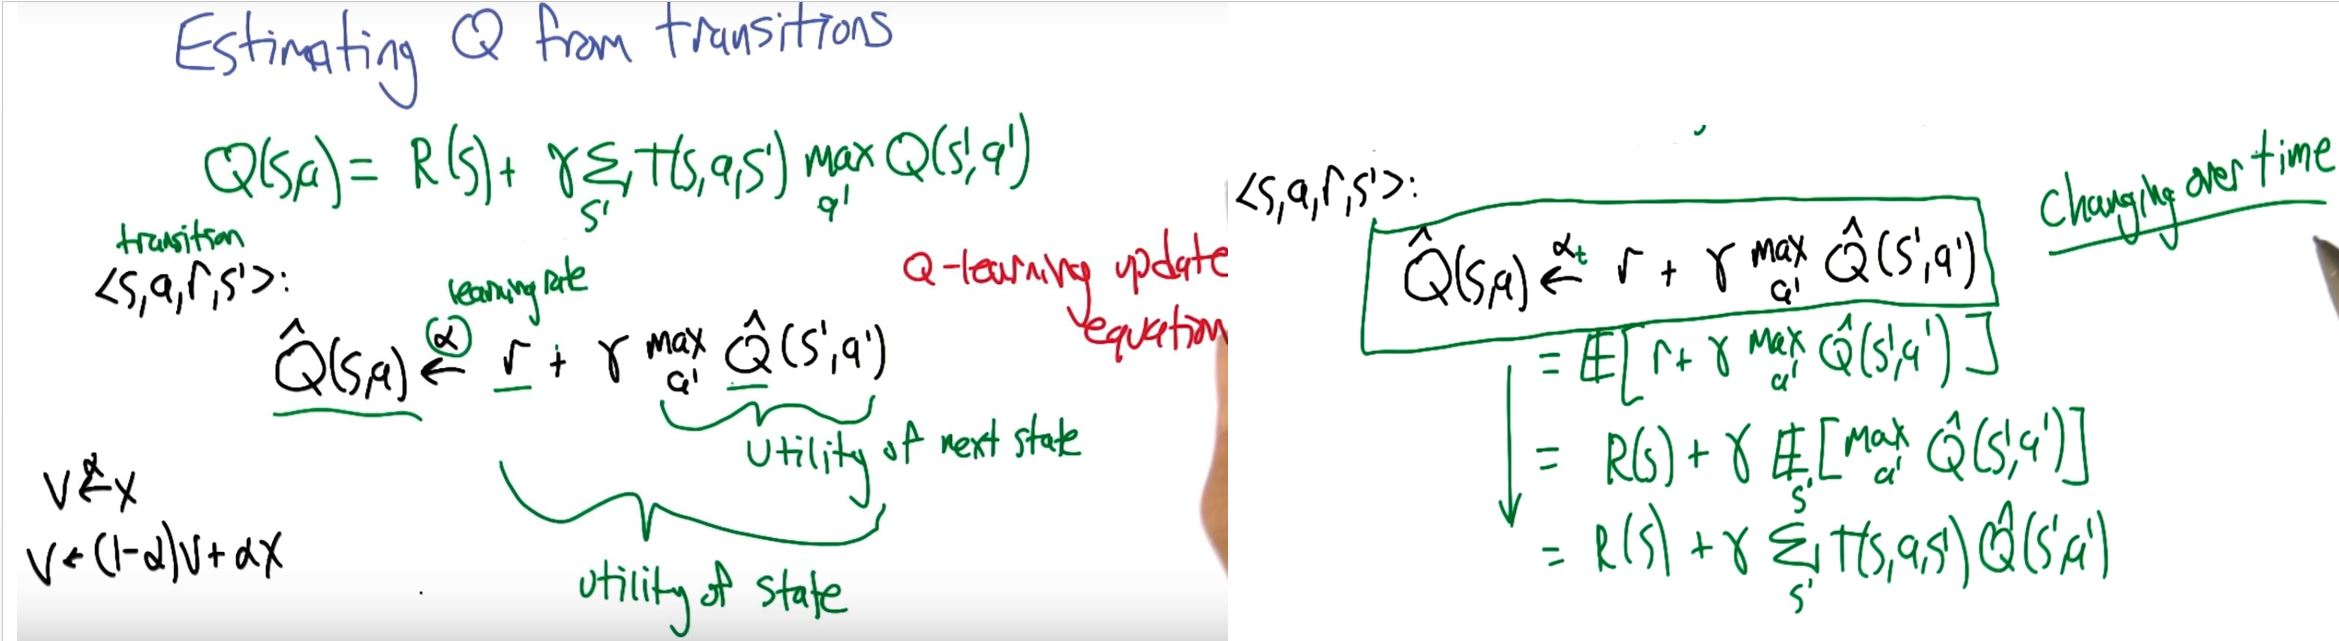
\includegraphics[width=0.9\textwidth]{pics/estimating_Q}
	\caption{Estimating Q from transitions} 
	\label{estimating_Q}
\end{figure}
%         -------------------------------------- 
The original proof of the Q-learning convergence (if you \textit{infinitely} visit all states) is \href{http://www.gatsby.ucl.ac.uk/~dayan/papers/cjch.pdf}{here}.

How do we choose actions? Choosing same action won't learn, just randomly selecting them is not enough - but a 'simulated annealing' approach type does: every once in a while introduce randomness to explore the whole space (greedly, local min) to visit states an infinitely amount of times (\textbf{$\epsilon$-greedy exploration}). \textbf{Exploration-Exploitation dilemma} or trade-off (whenever you learn by trying things out): the dilemma is between choosing what you know and getting something close to what you expect (‘exploitation’) vs. choosing something you are not sure about and possibly learning more (‘exploration’) - optimal learning requires that you sometimes make some bad choices (‘sub-optimal’ actions are necessary for your long term benefit). In model-based approaches, it is easier to use exploration (what model knows) and exploration (what can be learn) - in other words, this means going back and forth between model learning and planning (RL is the glue in between). \\
$\epsilon$: continuous (float) variable, whose default is 1, that controls the trade-off between exploitation and exploration: if a random probability is lower than the epsilon set value, then the agent will take a random action (exploitation), otherwise it will choose the best action (exploitation: highest Q-value for current state). It makes sense to start with a high epsilon in training (strong bias towards exploration) and update epsilon down (e.g. via a decay function) to move the bias towards exploitation (choosing best action after learning phase).   $\alpha$: continuous (float) value between 0 and 1, whose default set to 0.5, that represents the learning rate to be experienced by the agent - 0 (zero) means that the agent is not learning anything new, 1 that it only learns/considers the most recent information disregarding the past, values in between balance/weight between past and recent information (relative importance of past vs new info).\\
The concept of Q-Learning is fairly straightforward: for every state the agent visits, create an entry in the Q-table for all state-action pairs available. Then, when the agent encounters a state and performs an action, update the Q-value associated with that state-action pair based on the reward received and the iterative update rule implemented.

More details can be found in this \href{https://www.cs.cmu.edu/afs/cs/project/jair/pub/volume4/kaelbling96a.pdf}{survey paper}.
%%%%%%%%%%%%%%%%%%%%%%%%%%%%%%%%%%%%%%%%%%%%%%%%%%%%%%
\subsection{Game theory}
Different definitions for game theory:
\begin{itemize}
	\item mathematics of conflict
	\item from single agent (previous section) to multiple agents
	\item economics (origin of the theory)
	\item increasingly a part of AIML
\end{itemize}

Strategy: mapping of all states to  actions (called 'policy' in MDP for 1 agent) 

A simple game: \textit{\textbf{2-player zero-sum} finite deterministic \textbf{game} of \textbf{perfect} information}. It can be represented as a tree of decisions or, better, a matrix with final rewards as values (often called payoff matrix): one agent makes a move and the second follows (in a matrix one agent chooses the row and the other the column) with each agent trying to \textit{mini}mizing one's own possible loss for a worst case (\textit{max}imum loss) scenario (or minimizing the opponent's maximum payoff): \textbf{minimax} strategy. In such 2-player game, minimax is maxmin and there \textit{always exists} an \textit{optimal} \textit{pure} strategy for each player (where best row anf best column cross). Such result is still true if we assume that games are not \textbf{non-deterministic} (a result due to Von Neumann).

We can relax further our 2-player games by removing perfect information (which means that the choices by one player are not seen by the other player before making a decision - e.g. poker game - see left-side in fig. \ref{mixed_strategy}). In this case - with \textbf{hidden information} - minimax is different from maxmin. We now have to deal with \textbf{mixed strategies} (vs. pure ones when information was perfect): in a pure strategy you choose one strategy over (an)other(s), whilst mixed strategies imply a distribution over strategies (select either extremes, first or last, or max if they intersect - see right-side in the same fig.).
%          --------   FIGURE: mixed strategy  -----------
\begin{figure}[htbp] 
	\centering
	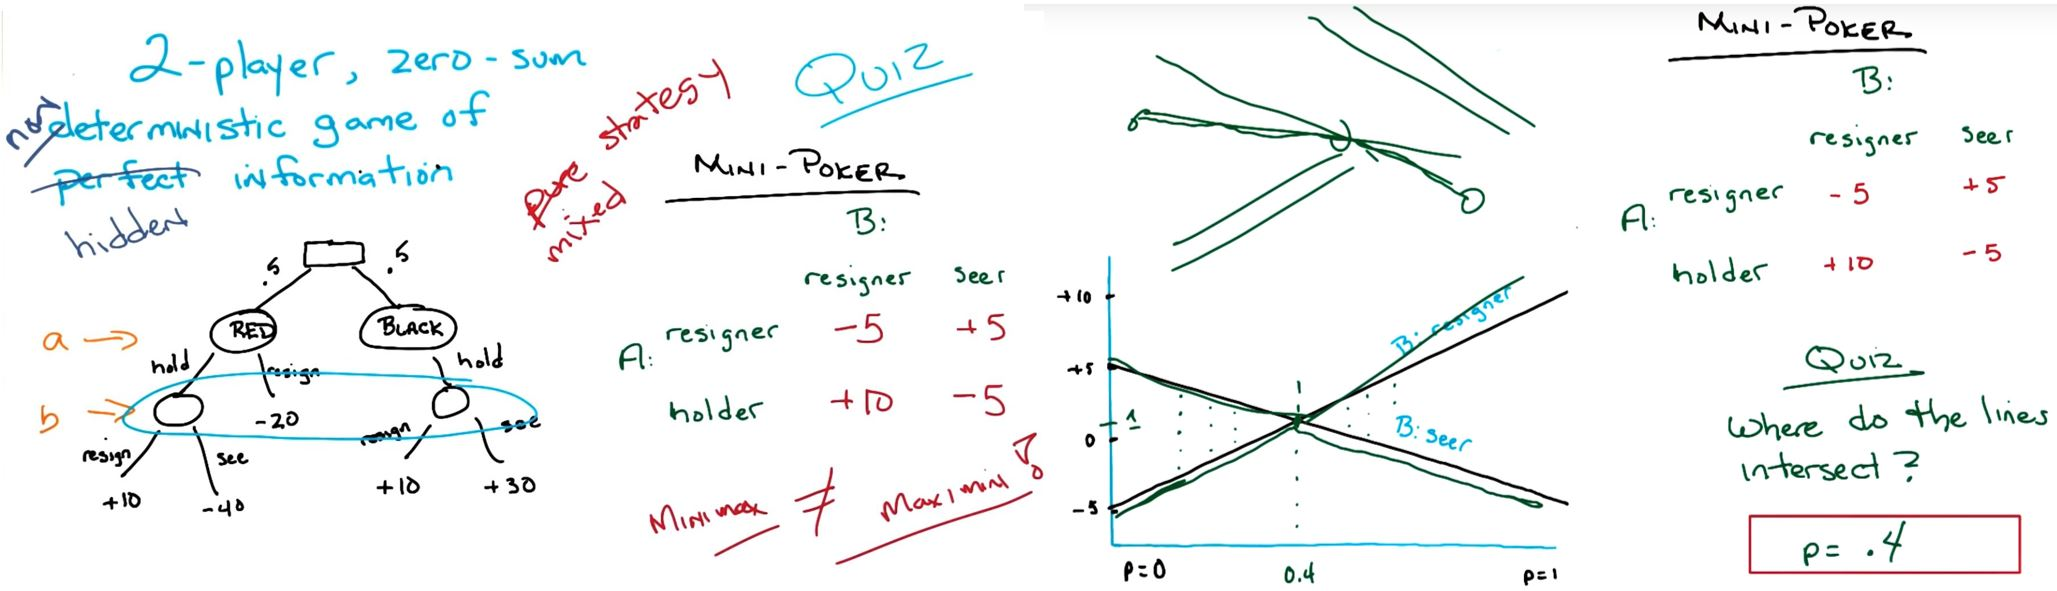
\includegraphics[width=0.9\textwidth]{pics/mixed_strategy}
	\caption{Mixed strategy: hidden information} 
	\label{mixed_strategy}
\end{figure}
%         -------------------------------------- 

Finally, let's relax the non-zero sum game. A classical example of game is the famous prisoner's dilemma where (sum of) rewards are not constant across different states (non-zero game indeed means that the sum of rewards of the game are constant, non necessarily zero.): the best solution seems to be for the two prisoners to cooperate between themselves, but if you know the opponent is going to cooperate then it is better to defect (report the other prisoner) and same if you know that is going to defect - so the dominant strategy is for both to defect. 

This leads us to the \textbf{Nash Equilibrium (NE)}: 
% \begin{theorem} test \end{theorem}
given $n$ players with strategies $S_1, S_2, \ldots, S_n$, then 
$S^*_1 \in S_1, S^*_2 \in S_2, \ldots, S^*_n \in S_n$ are Nash equilibrium if and only if $\forall \; i \;\; S^*_i=argmax_{S_i} \; \text{Utility}(S^*_1, \ldots,S^*_i, \ldots, S^*_n)$.
In words, we are in equilibrium if no player can gain by changing his strategy if the strategies of the others remain unchanged. Main NE facts:
\begin{itemize}
	\item In the n-player \textit{pure} strategy game, if elimination of strictly dominated strategies leaves just one combination, that combo is the unique NE.
	\item Any NE will survive elimination of strictly dominated strategies.
	\item if $n$ is finite and $\forall i \; S_i \exists \text{(mixed) NE}$
\end{itemize}

If the prisoner's dilemma game is played not once but more times, prisoners still defect - that is easy to see if you start from the end: even assuming $n-1$ games where prisoners both cooperated, the NE on the last game is for both to defect - but that is also the NE for the last but one game and so on. Hence no cooperation is possible and we are still trapped in the prisoners' dilemma. In short - in a $n$ repeated game, one gets $n$ repeated NE. In real-life, prisoners may cooperate because utilities are not just functions of their time in jail, but also of the time their friends spend in jail too. In addition, games are changed to avoid such a dilemma (\textbf{mechanism design}): even if you get out of jail at the expense of your fellow, then you get punished by their gangs - this is the same mechanism used in Economics (incentives to have people follow certain rules).

\subsubsection{Stochastic games}
Stochastic (or Markov) games are a formal model/framework for \textit{multi-agent} reinforcement learning.

Let's re-define the framework, as per section \ref{mdp}, for the 2-players case:
\begin{itemize}
	\item \textbf{states}: $s$;
	\item \textbf{actions} for player $i$: $a, b$, where $a \in A_1$ and $b \in A_2$ ;
	\item \textbf{transitions}: $T(s, (a, b),s')$, note joint action;
	\item \textbf{reward} for player $i$: $R_1(s, (a,b))$, $R_2(s, (a,b))$
	\item \textbf{discount}: $\gamma$, same for both (but no needed to be).
\end{itemize}
This model, which is a generalisation of MDP, was published by Nobel-price winner Shapley \textit{before} Bellmann published about MDP. Note that MDP is like Stochastic Games when the other player's actions are irrelevant.

We can extend Q-Learning of MDP to zero-sum Stochastic games: minimax-Q (fig. \ref{minimax_Q} for eq. and its properties).
%          --------   FIGURE: minimax-Q  -----------
\begin{figure}[htbp] 
	\centering
	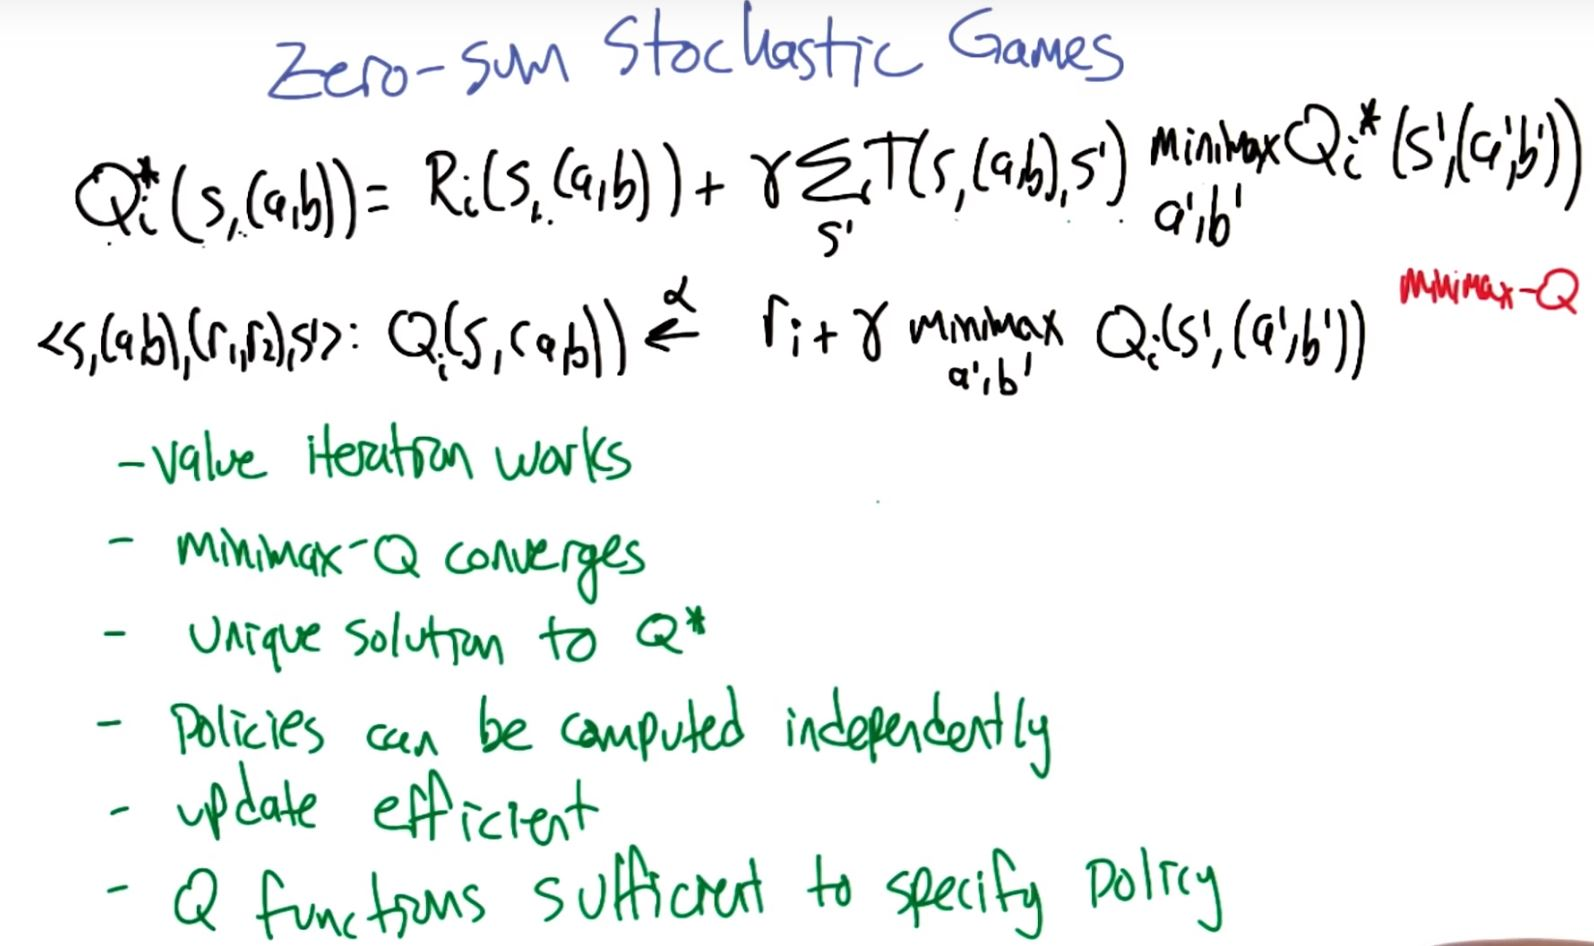
\includegraphics[width=0.7\textwidth]{pics/minimax_Q}
	\caption{Zero-sum stochastic games: minimax-Q} 
	\label{minimax_Q}
\end{figure}
%         --------------------------------------

For general (ie. non-zero-sum) stochastic games we may use Nash equilibrium rather than minimax (which does not work for non-zero games) for learning, but properties are much worse (fig. \ref{general_games}).
%          --------   FIGURE: Nash-Q  -----------
\begin{figure}[htbp] 
	\centering
	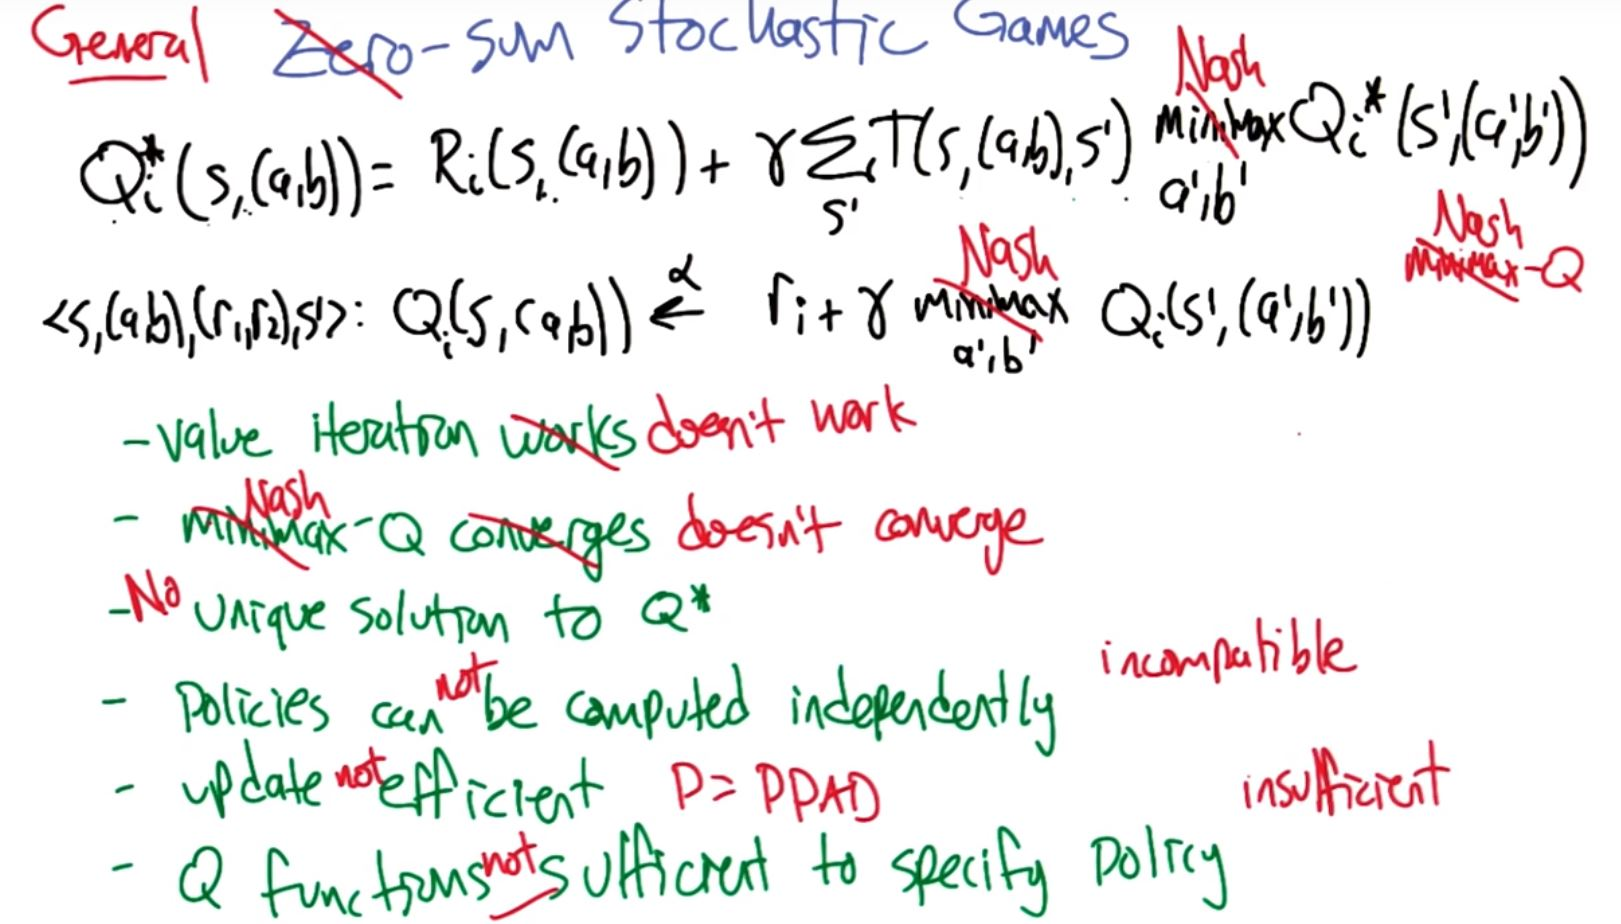
\includegraphics[width=0.7\textwidth]{pics/general_games}
	\caption{General stochastic games: Nash-Q} 
	\label{general_games}
\end{figure}
%         --------------------------------------	
There are different ways to address the issue to solve stochastic games to get closer to solve them:
\begin{itemize}
	\item repeated stochastic games (Folk theorem);
	\item cheap talk that may lead to correlated equilibria;
	\item cognitive hierarchy that leads to best responses;
	\item side payments (coco values).
\end{itemize}

 
%%%%%%%%%%%%%%%%%%%%%%%%%%%%%%%%%%%%%%%%%%%%%%%%%%%%%%
%	DEEP LEARNING
%%%%%%%%%%%%%%%%%%%%%%%%%%%%%%%%%%%%%%%%%%%%%%%%%%%%%%
\section{Deep Learning (Keras, Tensorflow)}	\label{deep_learning}
Start first by review sections the above sections on perceptrons \ref{perceptrons} and Softmax \ref{multinominal}, in particular perceptron and gradient descent algorithms\footnote{A well written, free, extra resource for more details is \href{http://neuralnetworksanddeeplearning.com/}{deep learning book}.}.

Now were are in a position to put all the building blocks together and start from Neural Networks.

%%%%%%%%%%%%%%%%%%%%%%%%%%%%%%%%%%%%%%%%%%%%%%%%%%%%%%
\subsection{Neural Networks intro}
To start building neural networks ('NN'), we combine two perceptrons (whose outputs are \textit{linear} boundaries) into a third model that gets us \textit{nonlinear} boundaries - e.g. summing the two probabilities generated by the two perceptrons and use the sigmoid function to turn the such a sum into a probability (we can also use weights to assign more importance to one perceptron over the other). 

We can enrich the NN architecture further by either:
\begin{itemize}
	\item \underline{adding more \textbf{nodes}} to the (i) input layer (very first layer: space dimensions), (ii) hidden layer (the set of linear models created by the inputs), and (iii) output layer (which combines the previous linear models to get a non-linear one - if it has a single node - or a \textit{multi-class classification} if more nodes are added) - see fig \ref{neural_network_simple}) - and/or
	\item \underline{add more \textbf{layers}}, which is where the 'deep' NN magic happens.
\end{itemize}
%          --------   FIGURE: neural_network_simple  -----------
\begin{figure}[htbp] 
	\centering
	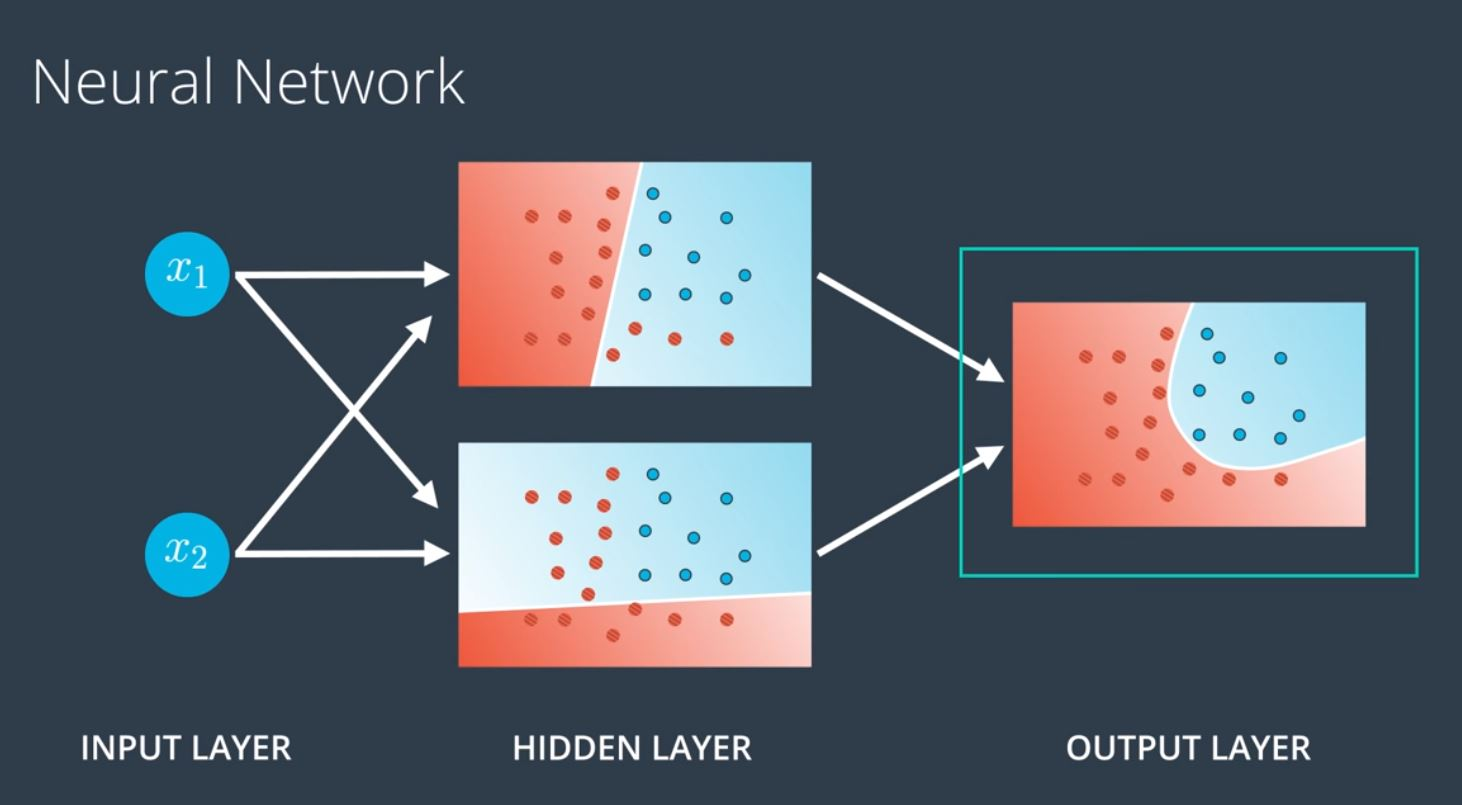
\includegraphics[width=0.7\textwidth]{pics/neural_network_simple}
	\caption{Simple Neural Network architecture} 
	\label{neural_network_simple}
\end{figure}
%         --------------------------------------
In other words, neural networks are a bunch of perceptrons added together in parallel to form one layer and multiplying such layers separated by non-linear elements.

To recap: neural network can represent booleans, continuous or arbitrary functions by just adding more \textbf{units} (more perceptrons, e.g. visually organised in a column) and (hidden) \textbf{layers} (number of columns) - so no restriction bias. To avoid overfit than limit numbers of units/layers and use cross-validation (same the trade-off bias vs. variance in other methods.)

\textbf{Feedforward} is the process neural networks use to turn the inputs into an output: it takes the input vector and apply a sequence of linear models (vector and matrix multiplication) and sigmoid functions to return predictions (see fig. \ref{feedforward})
%          --------   FIGURE: feedforward  -----------
\begin{figure}[htbp] 
	\centering
	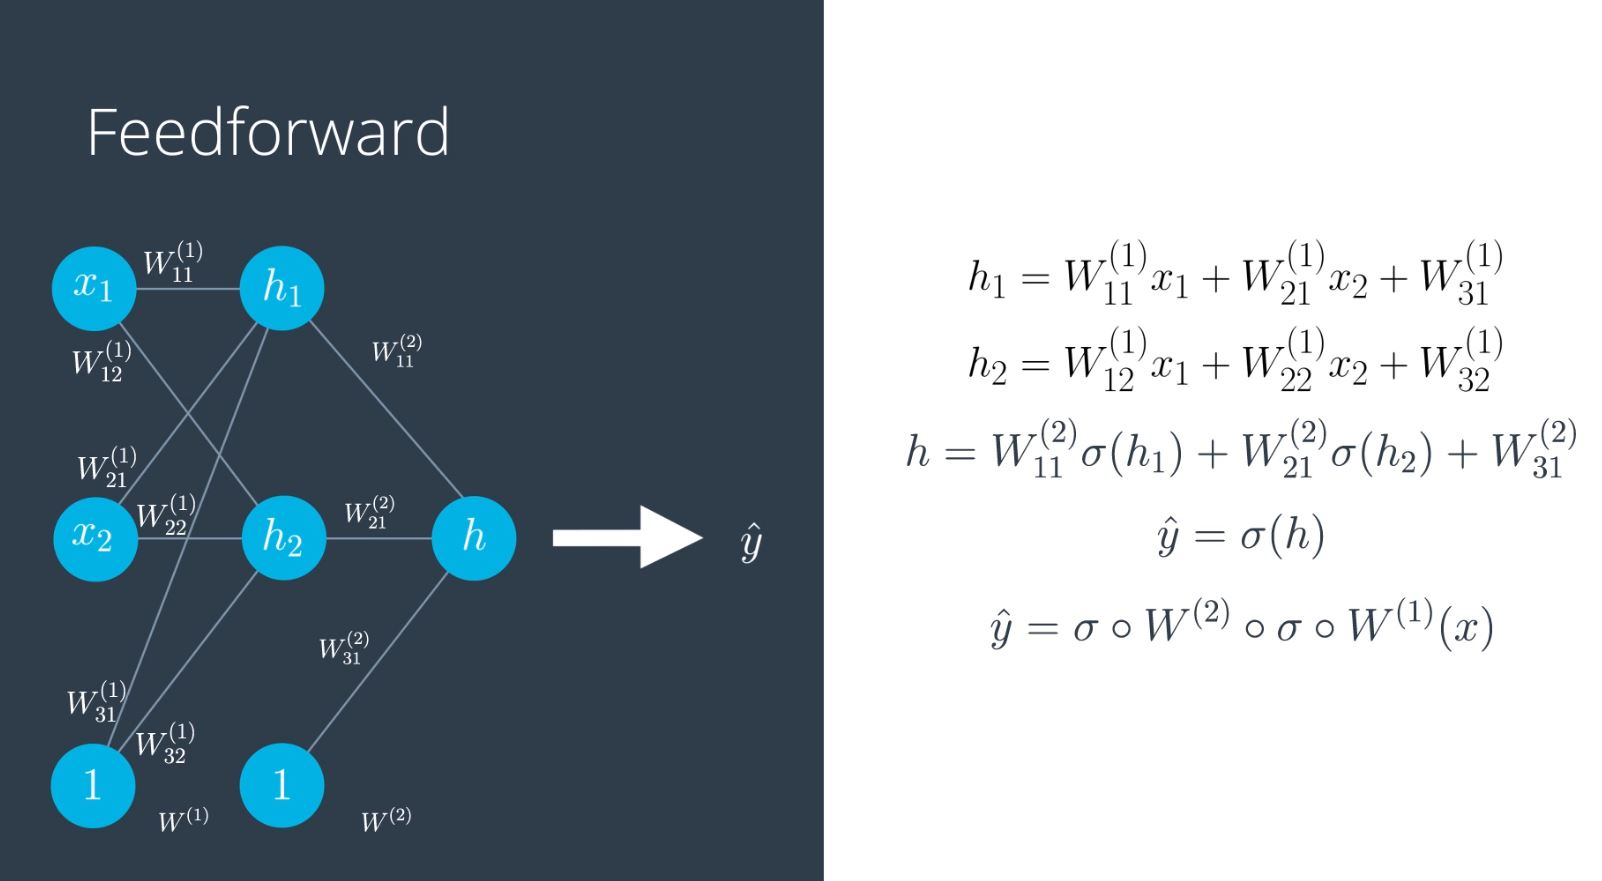
\includegraphics[width=0.8\textwidth]{pics/feedforward}
	\caption{Feedforward} 
	\label{feedforward}
\end{figure}
%         --------------------------------------

Just as before, neural networks will produce an error function, which at the end, is what we'll be minimizing to train a NN.

\textbf{Backpropagation}: get output given inputs by changing intermediate units and layers using gradient descent (one at the time).

In a nutshell, backpropagation consists of:
\begin{itemize}
	\item Running the feedforward operation.
	\item Comparing the output of the model with the desired output and calculating the error.
	\item Running the feedforward operation \textit{backwards} (backpropagation) to spread the error to each of the weights.
	\item Use this to update the weights, and get a better model.
	\item Repeat this until we have a model that is good.
\end{itemize}

We already did the math for the \underline{single perceptron case} in the 'Gradient aside' part of sect. \ref{multinominal}; for the \underline{multi-layer perceptron} the math is similar but a bit more complicated:
\begin{itemize}
	\item prediction: $\hat{y} = \sigma W^{(3)} \circ \sigma W^{(2)} \circ \sigma \circ W^{(1)}(x)$, a composition of functions;
	\item error function: similar, but with more complicated predictions;
	\item gradient of the error function:  similar, but longer vector.
\end{itemize}
%          --------   FIGURE: backpropagation1  -----------
\begin{figure}[htbp] 
	\centering
	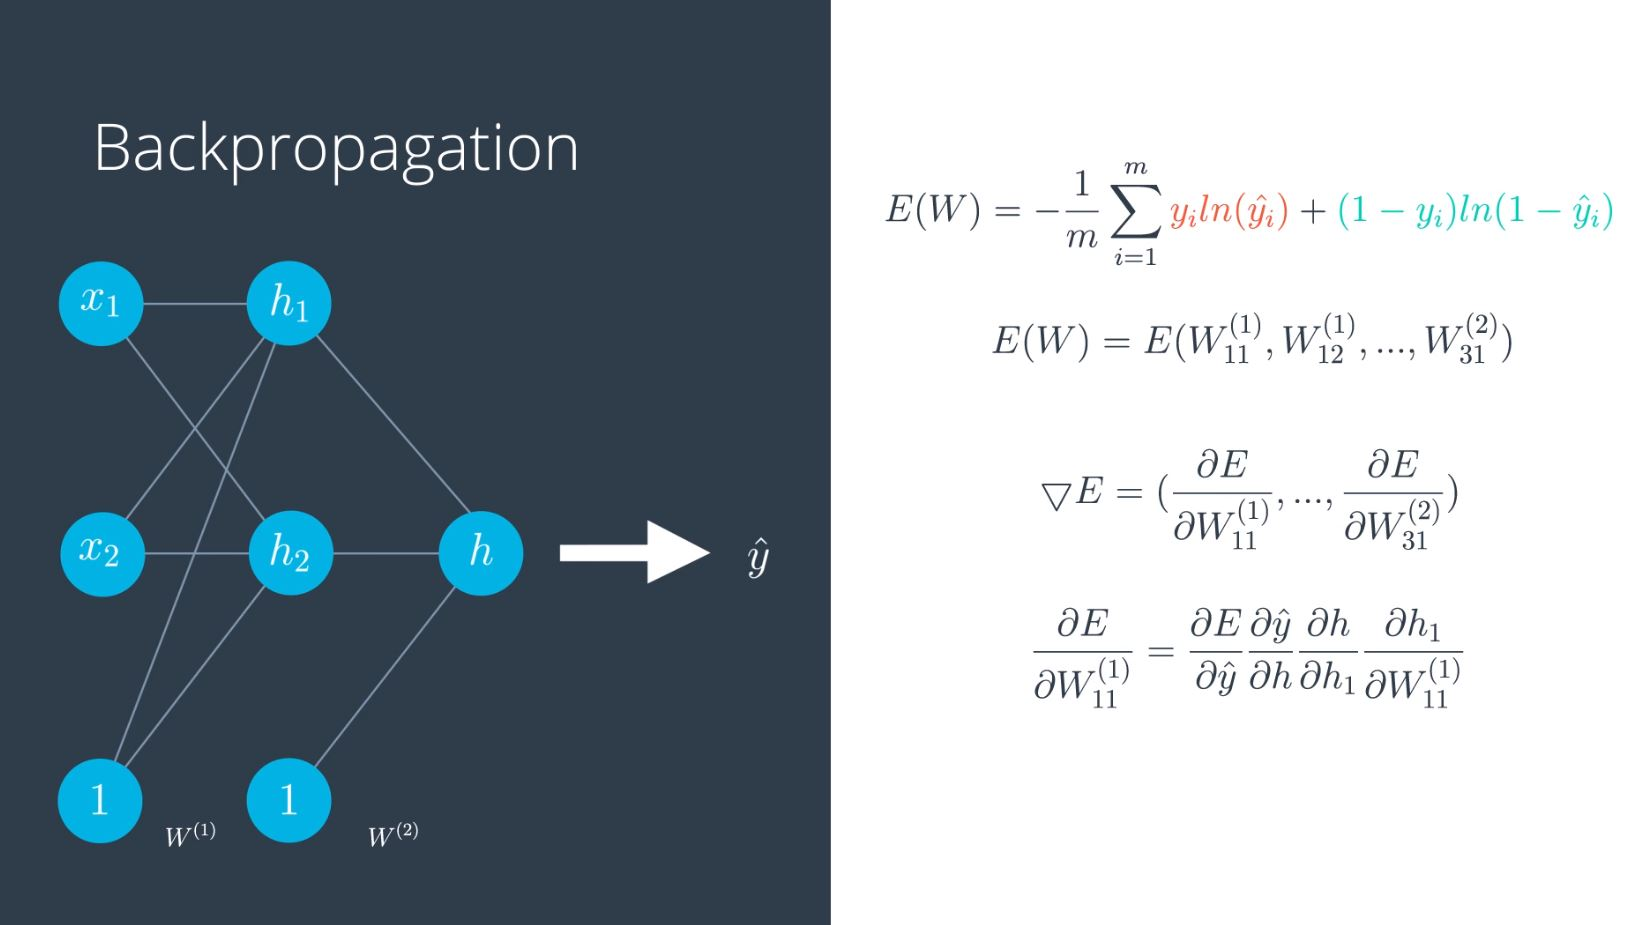
\includegraphics[width=0.8\textwidth]{pics/backpropagation1}
	\caption{Backpropagation} 
	\label{backpropagation1}
\end{figure}
%         --------------------------------------
%          --------   FIGURE: backpropagation2  -----------
\begin{figure}[htbp] 
	\centering
	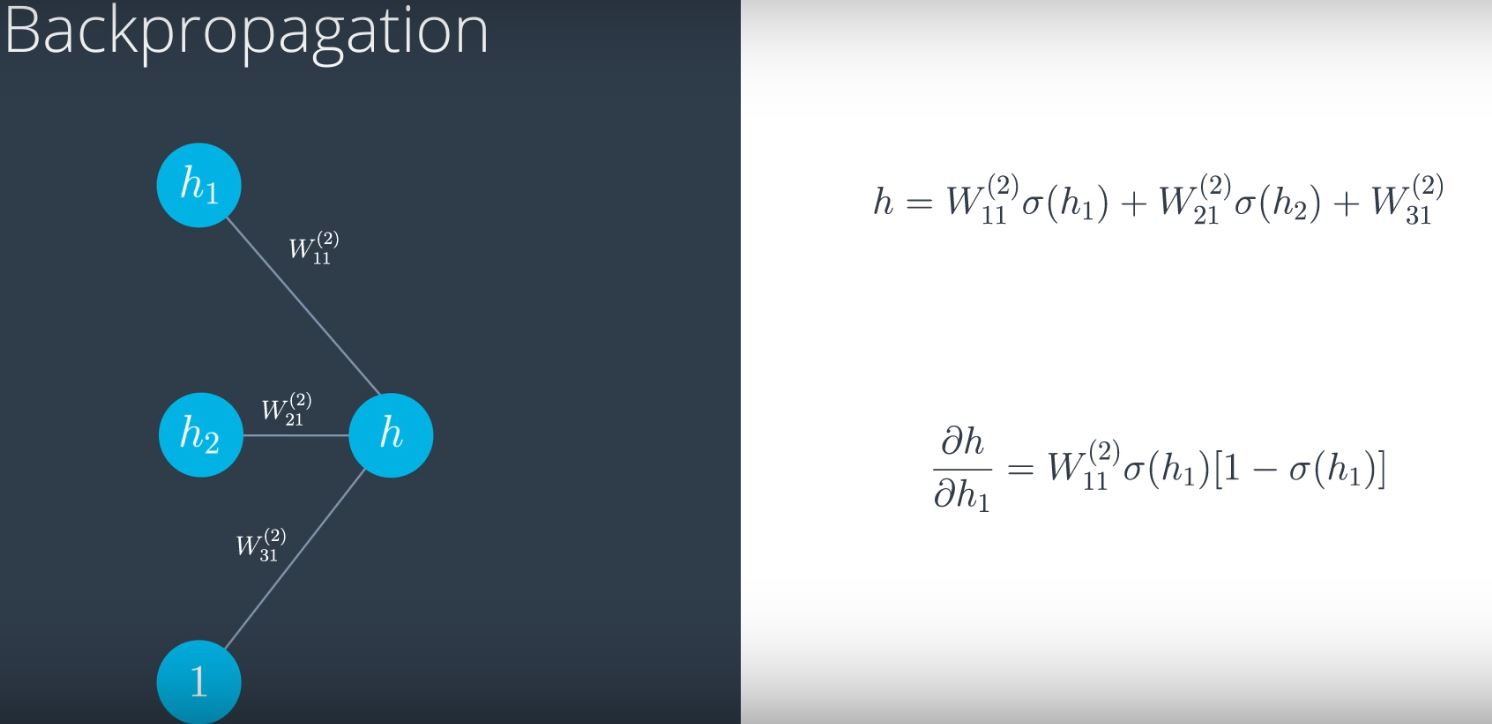
\includegraphics[width=0.7\textwidth]{pics/backpropagation2}
	\caption{Backpropagation - example of derivation} 
	\label{backpropagation2}
\end{figure}
%         --------------------------------------

Preference bias: algorithm's selection of one representation over another. Occam's razor.

%%%%%%%%%%%%%%%%%%%%%%%%%%%%%%%%%%%%%%%%%%%%%%%%%%%%%%
\subsection{Keras}
Keras is a high-level neural networks API, written in Python, and capable of running on top of TensorFlow (preferable), (Microsoft) CNTK, or Theano.

Unless for research purposes or developing special neural networks, Keras is the better choice since you can quickly build even very complex models. If more control over the network or debugging / watch closely is required, TensorFlow ('TF') is the right choice (though the syntax can be sometimes a nightmare)\footnote{Since Keras is going to be integrated in TF, it is likely wiser to build your network using tf.contrib.Keras and insert anything you want in the network using pure TensorFlow}.

The general idea for this example is that you'll first load the data, then define the network, and then finally train the network.
\begin{lstlisting}
import numpy as np
from keras.utils import np_utils
import tensorflow as tf
# Using TensorFlow 1.0.0; use tf.python_io in later versions
tf.python.control_flow_ops = tf

# Set random seed
np.random.seed(42)

# a wrapper that treats the network as a sequence of layers
# common methods are compile(), fit(), and evaluate()
from keras.models import Sequential
from keras.layers.core import Dense, Activation

# X has shape (num_rows, num_cols), where the training data stored
# as row vectors
X = np.array([[0, 0], [0, 1], [1, 0], [1, 1]], dtype=np.float32)
    
# y must have an output vector for each input vector
y = np.array([[0], [0], [0], [1]]).astype('float32')

# One-hot encoding the output
y = np_utils.to_categorical(y) # , num_classes=1)
# or no need for the above and use 'binary_crossentropy'
    
# Create the Sequential model
model = Sequential()
    
# 1st Layer - Add an input layer of 32 nodes with same input shape 
# as the training samples in X
model.add(Dense(32, input_dim=X.shape[1]))
    
# Add a softmax activation layer
model.add(Activation('softmax'))  # or 'tanh', ...

# two steps above are equivalent to: 
# model.add(Dense(32, activation="softmax")))
# but common to separate the two for direct access

# 2nd Layer - Add a fully connected output layer (dim=1)
model.add(Dense(1)) # since only two classes: 0 and 1
    
# Add a sigmoid activation layer
model.add(Activation('sigmoid'))

# call backend and binds loss fnc, optimiser and metrics
model.compile(loss="categorical_crossentropy", 
			 optimizer="adam", metrics = ["accuracy"])
# see resulting model architecture
model.summary()

# train the model
model.fit(X, y, nb_epoch=1000, verbose=0)
# nb: in Keras 2 'nb_epoch' becomes 'epochs'

# if train and test, and batch_size
model.fit(x_train, y_train, epochs=10,  
	batch_size=32,	verbose=2,
	validation_data=(x_test, y_test))

# finally see how the model does
score = model.evaluate(X, y)
print('Test loss:', score[0])
print("\nAccuracy: ", score[-1])

# Checking the predictions
print("\nPredictions:")
print(model.predict_proba(X))
\end{lstlisting}
Keras requires the input shape to be specified in the first layer, but it will automatically infer the shape of all other layers. This means you only have to explicitly set the input dimensions for the first layer.

Once we have our model built, we need to compile it before it can be run on any input data. Compiling the Keras model calls the backend (Tensorflow - as default - or Theano, etc.) and binds the optimizer, loss function, and other parameters.

More examples - Multi-Layer Perceptrons '\textbf{MLP}' in Kears on MNIST dataset - can be found either \href{https://github.com/keras-team/keras/blob/master/examples/mnist_mlp.py}{here} - note 'reshape' of $x$ data or in appendix \ref{mln_on_mnist} where \textbf{flatten} was used.

Stochastic (mini-batch) gradient descent is very easy to implement in Keras. All we need to do is specify the size of the batches (\text{batch\_size}) in the training process, as follows:
\begin{lstlisting}
model.fit(X_train, y_train, epochs=1000, 
		  batch_size=100, verbose=0)
\end{lstlisting}
Its learning rate needs to be small: it takes more time, but less likely to overshoot and missing the minimum. Sometimes, just decreasing such a rate is the solution to improve a poorly performing model. 

Some terminology:
\begin{itemize}
	\item one \textbf{epoch} = one forward pass and one backward pass of \textit{all} the training examples;
	%
	\item \textbf{mini-batch} size = the number of training examples in one forward/backward pass. The higher the mini-batch size, the more memory space you'll need.	
	%
	\item number of \textbf{iterations} = number of passes, each pass using [mini-batch size] number of examples. To be clear, one pass = one forward pass + one backward pass (we do not count the forward pass and backward pass as two different passes).
\end{itemize}
Example: if you have 1000 training examples, and your mini-batch size is 500, then it will take 2 iterations to complete 1 epoch.

Difficult bias-variance trade-off for neural network: increases \textbf{epochs}  improves fitting (lower bias), but after some values it start to overfit the data. Some solutions  for reducing overfitting are:
\begin{itemize}
	\item \textbf{early stopping} algorithm in neural network: no. of epochs to be used are those where the testing error stops decreasing and starts increasing.
	% 
	\item \textbf{L-norm regularisations} (penalise larger weights): either (i) \textbf{L1} (i.e. by adding $\lambda \sum_i |w_i|$ to the error function - as in LASSO regression) which produces \textit{sparse} (vector) weights and, hence, good for feature selection - or (ii) \textbf{L2} (i.e. by adding $\lambda \sum_i w^2_i$ - as in Ridge regression) which produces more \textit{homogeneous} weights and whose gradient is smoother\footnote{Think of a tangent to a diamond-shaped area in L1 vs. to a circle in L2 case.};
	%
	\item \textbf{dropout} is a popular regularisation technique in neural networks: units (for each hidden or visible layer) are randomly ignored (dropped out) during training  (for each training sample, for each iteration), with probability $p$, so that a reduced network is left, avoiding too higher weights in some parts of the net. In Keras, we can easily add a dropout after adding a layer as follows:
	\begin{lstlisting}
	model.add(Dense(32, activation='sigmoid'))
	model.add(Dropout(0.2))
	\end{lstlisting}
	The parameter here that is set at 0.2, is for the probability that each node gets dropped of. Thus, as we make each training pass over the data, each node gets dropped off with a probability of 0.2.
\end{itemize}


\textbf{Vanishing gradient} issue: gradient may get quite small in neural networks (see fig \ref{backpropagation3}).  
%          --------   FIGURE: vanishing gradient  -----------
\begin{figure}[htbp] 
	\centering
	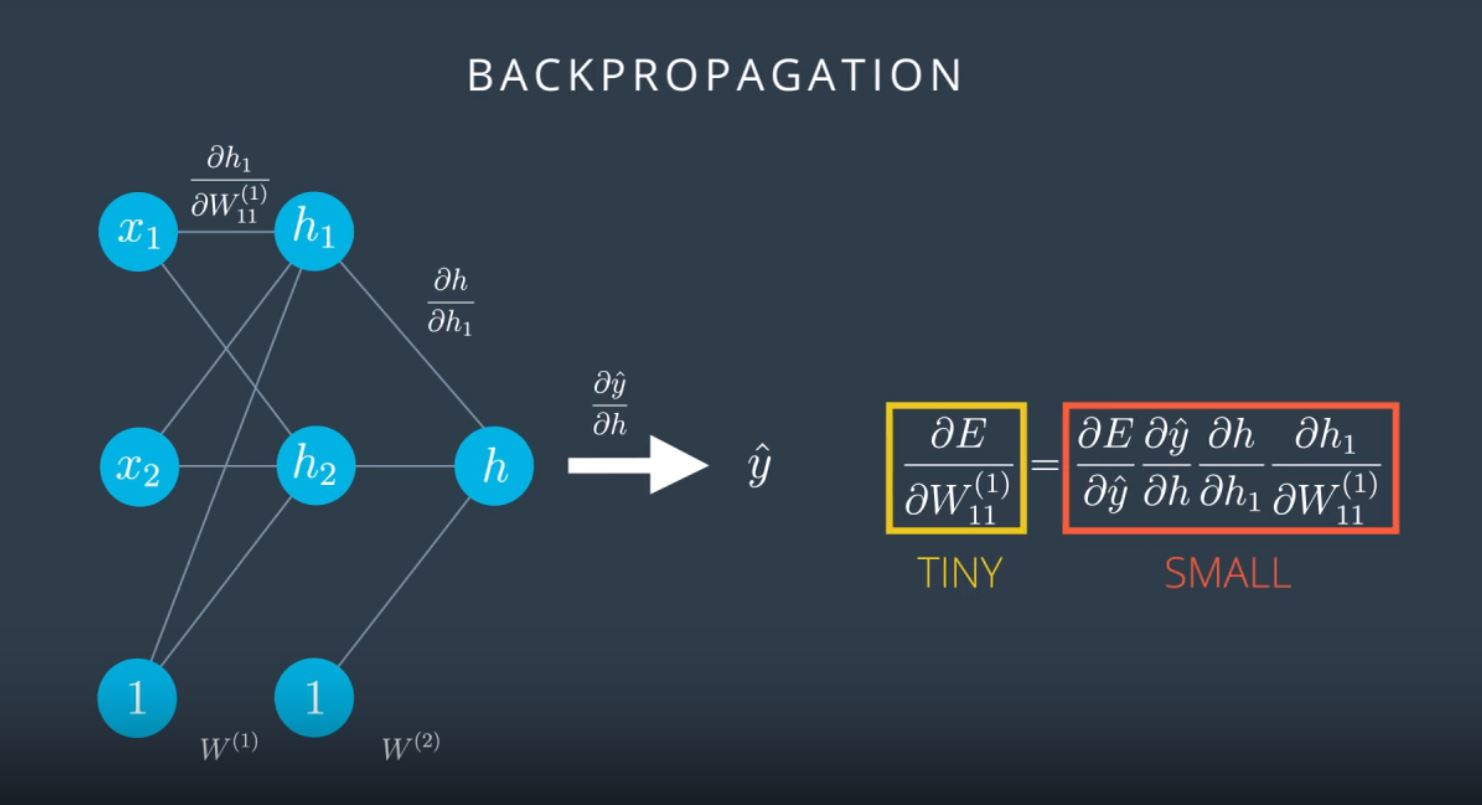
\includegraphics[width=0.7\textwidth]{pics/backpropagation3}
	\caption{Backpropagation - vanishing gradient} 
	\label{backpropagation3}
\end{figure}
%         --------------------------------------

One solution is to change the activation from (i) \textbf{sigmoid} function, $\sigma(x)=1/(1+e^{-x})$, to (ii) \textbf{hyperbolic tangent} function,  $tanh(x)=(e^{x}-e^{-x})/(e^{x}+e^{-x})$, or to (iii) rectified linear unit (\textbf{ReLU}), $relu(x) = x \; \text{if} \; x\geqslant0, \; 0 \; \text{otherwise}$\footnote{Which is nothing more than $\max(0,x$). This function is quite popular, more than the sigmoid - e.g ReLU in the intermediate layers and sigmoid in the output to get a probability.}. In Keras:
\begin{lstlisting}
# examples of different activation fncts:
model.add(Activation('sigmoid')) # two classes
model.add(Activation('softmax')) # more classes
model.add(Activation('relu'))
model.add(Activation('tanh'))
\end{lstlisting}

In order to avoid being stuck in a local minimum with SGD, one can use:
\begin{itemize}
	\item \textbf{random start}: simply start from different random places;
	\item \textbf{momentum}: exponential moving average of previous steps (fig. \ref{momentum});
\end{itemize}
%          --------   FIGURE: vanishing gradient  -----------
\begin{figure}[htbp] 
	\centering
	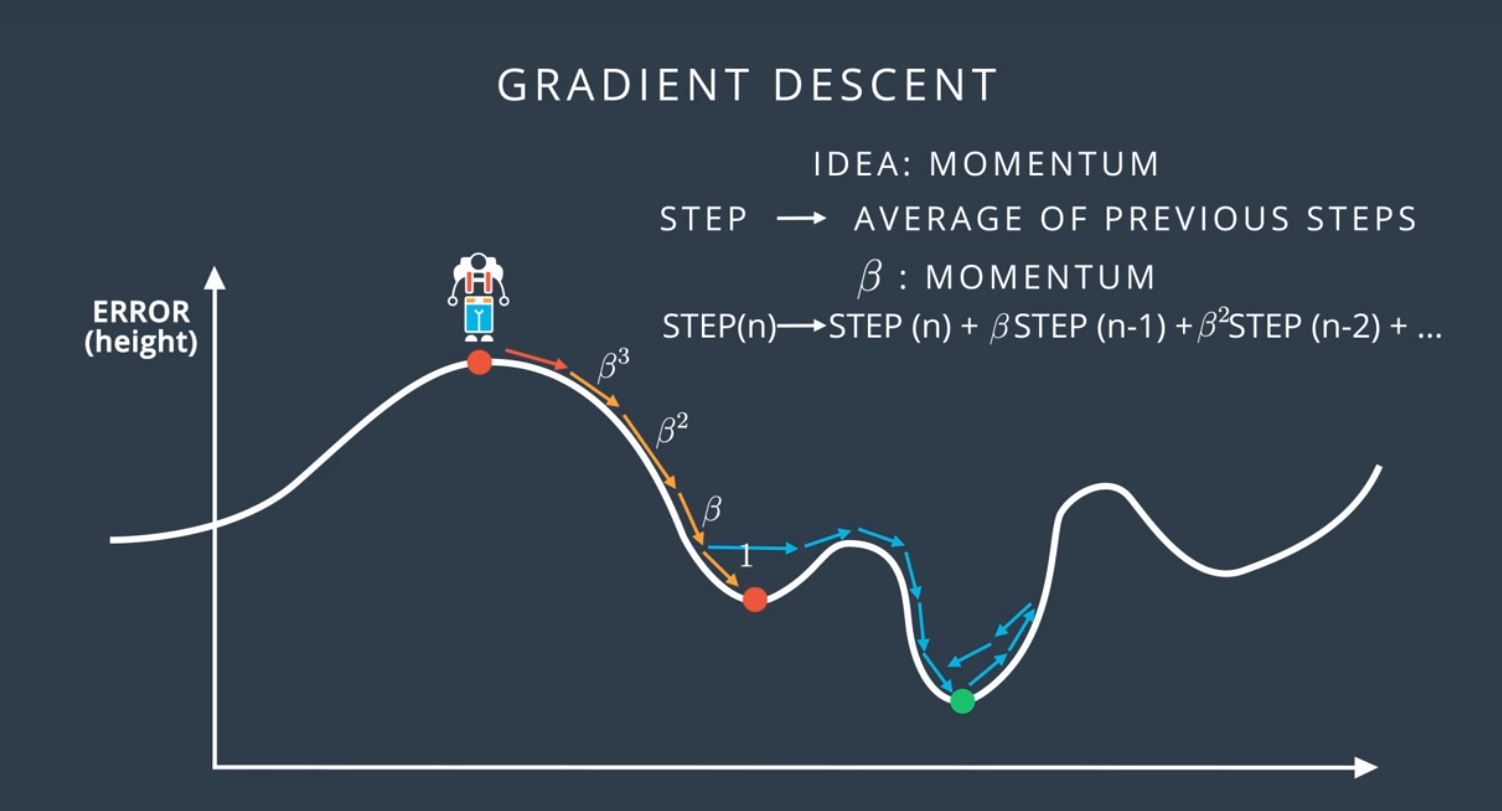
\includegraphics[width=0.7\textwidth]{pics/momentum}
	\caption{Momentum to overcoming local minima} 
	\label{momentum}
\end{figure}
%         --------------------------------------

There are many \textbf{optimisers} in Keras, most common being:
\begin{itemize}
	\item Stochastic Gradient Descent: using (i) learning rate, (ii) momentum and (iii) Nesterov momentum (which lowers down the gradient when it is closer to the solution).
	\item \textbf{Adam} (Adaptive Moment Estimation) uses a more complicated exponential decay that consists of not just considering the average (first moment), but also the variance (second moment) of the previous steps.
	\item \textbf{RMSProp} (Root Mean Squared Error prop) decreases the learning rate by dividing it by an exponentially decaying average of squared gradients.
\end{itemize}
See blog link in appendix \ref{gradient_descent} for more details.

There are some other error functions that we did not touch.

%%%%%%%%%%%%%%%%%%%%%%%%%%%%%%%%%%%%%%%%%%%%%%%%%%%%%%
\subsection{Convolutional Neural Networks (CNNs)}
Convolutional Neural Networks (ConvNets or CNNs) are a category of Neural Networks that have proven very effective in areas such as image recognition (identifying faces, handwritten digits, people/signs for self-driving cars, etc) and classification. 

Contrary to MLPs where data are vectors (e.g. square pics of digits are flattened in vectors of black, grey and whites), CNNs really shines with real data, e.g. when images are not standardised as in the MNIST dataset.

Similarly MLPs and CNNs are composed of stacked layers (input, hidden, outputs) and use same optimisers for loss function, byt \textbf{types of hidden layers} for the latter are different (convolution, pooling, fully connected layers).

%%%%%%%%%%%%%%%%%%%%%%%%%%%%%%%%%%%%%%%%%%%%%%%%%%%%%%
\subsubsection{Hyperparameters search with Keras}
Hyperparameter optimization is a big part of deep learning: neural networks are notoriously difficult to configure and there are a lot of parameters that need to be set (batch size and epoch, learning rate, activation function, weight initialisation, drop out, neurons in the hidden layers).

We can use the grid search (\textbf{GridSearchCV} class) from the scikit-learn library to tune the hyperparameters of Keras deep learning models, by wrapping such models with the \textbf{KerasClassifier} or \textbf{KerasRegressor} class.

One must provide a dictionary of hyperparameters to evaluate in the \textbf{param\_grid} argument (array of values to try). By setting the n\_jobs argument to $-1$, process will use all cores on your machine. Cross validation is used to evaluate each individual model and the default of 3-fold cross validation is used (although this can be overridden by specifying the \textbf{cv} argument).

Example to tune batch size and epoch number (source is \href{https://machinelearningmastery.com/grid-search-hyperparameters-deep-learning-models-python-keras/}{here}, also for more examples):
\begin{lstlisting}
# Use scikit-learn to grid search the batch size and epochs
import numpy
from sklearn.model_selection import GridSearchCV
from keras.models import Sequential
from keras.layers import Dense
from keras.wrappers.scikit_learn import KerasClassifier
# Function to create model, required for KerasClassifier
def create_model():
	# create model
	model = Sequential()
	model.add(Dense(12, input_dim=8, activation='relu'))
	model.add(Dense(1, activation='sigmoid'))
	# Compile model
	# optimizer = SGD(lr=learn_rate, momentum=momentum)
	model.compile(loss='binary_crossentropy', 
		optimizer='adam', metrics=['accuracy'])
	return model

# fix random seed for reproducibility
numpy.random.seed(7)

# load dataset
dataset = numpy.loadtxt("pima-indians-diabetes.csv", delimiter=",")

# split into input (X) and output (Y) variables
X = dataset[:,0:8]
Y = dataset[:,8]

# create model
model = KerasClassifier(build_fn=create_model, verbose=0)

# define the grid search parameters
batch_size = [10, 20, 40, 60, 80, 100]
epochs = [10, 50, 100]
param_grid = dict(batch_size=batch_size, epochs=epochs)

# other hyperparams ... need to change model fnct above
# optimizer = ['SGD', 'RMSprop', 'Adagrad', 'Adadelta', 
			'Adam', 'Adamax', 'Nadam']
# learn_rate = [0.001, 0.01, 0.1, 0.2, 0.3]
# momentum = [0.0, 0.2, 0.4, 0.6, 0.8, 0.9]

grid = GridSearchCV(estimator=model, param_grid=param_grid, n_jobs=-1)
grid_result = grid.fit(X, Y)

# summarize results
print("Best: %f using %s" % (grid_result.best_score_, 			
		grid_result.best_params_))
means = grid_result.cv_results_['mean_test_score']
stds = grid_result.cv_results_['std_test_score']
params = grid_result.cv_results_['params']

for mean, stdev, param in zip(means, stds, params):
	print("%f (%f) with: %r" % (mean, stdev, param))
\end{lstlisting}

%%%%%%%%%%%%%%%%%%%%%%%%%%%%%%%%%%%%%%%%%%%%%%%%%%%%%%
\subsubsection*{Local connectivity}
\textbf{MLPs} has two main \textbf{limitations}: (i) only use \textbf{fully} connected layers (hence a lot of parameters) and (ii) only accept \textbf{vectors} as inputs (losing the actual position of the pixels in a matrix). CNNs will address these issues by also (i) using \textbf{sparsely} connected layers (\textit{locally} connecting some pixels to some hidden nodes, not all to all) and (ii) accept \textbf{matrices} as inputs - see fig. \ref{CNN_local_connectivity}.

%          --------   FIGURE: local connectivity  -----------
\begin{figure}[htbp] 
	\centering
	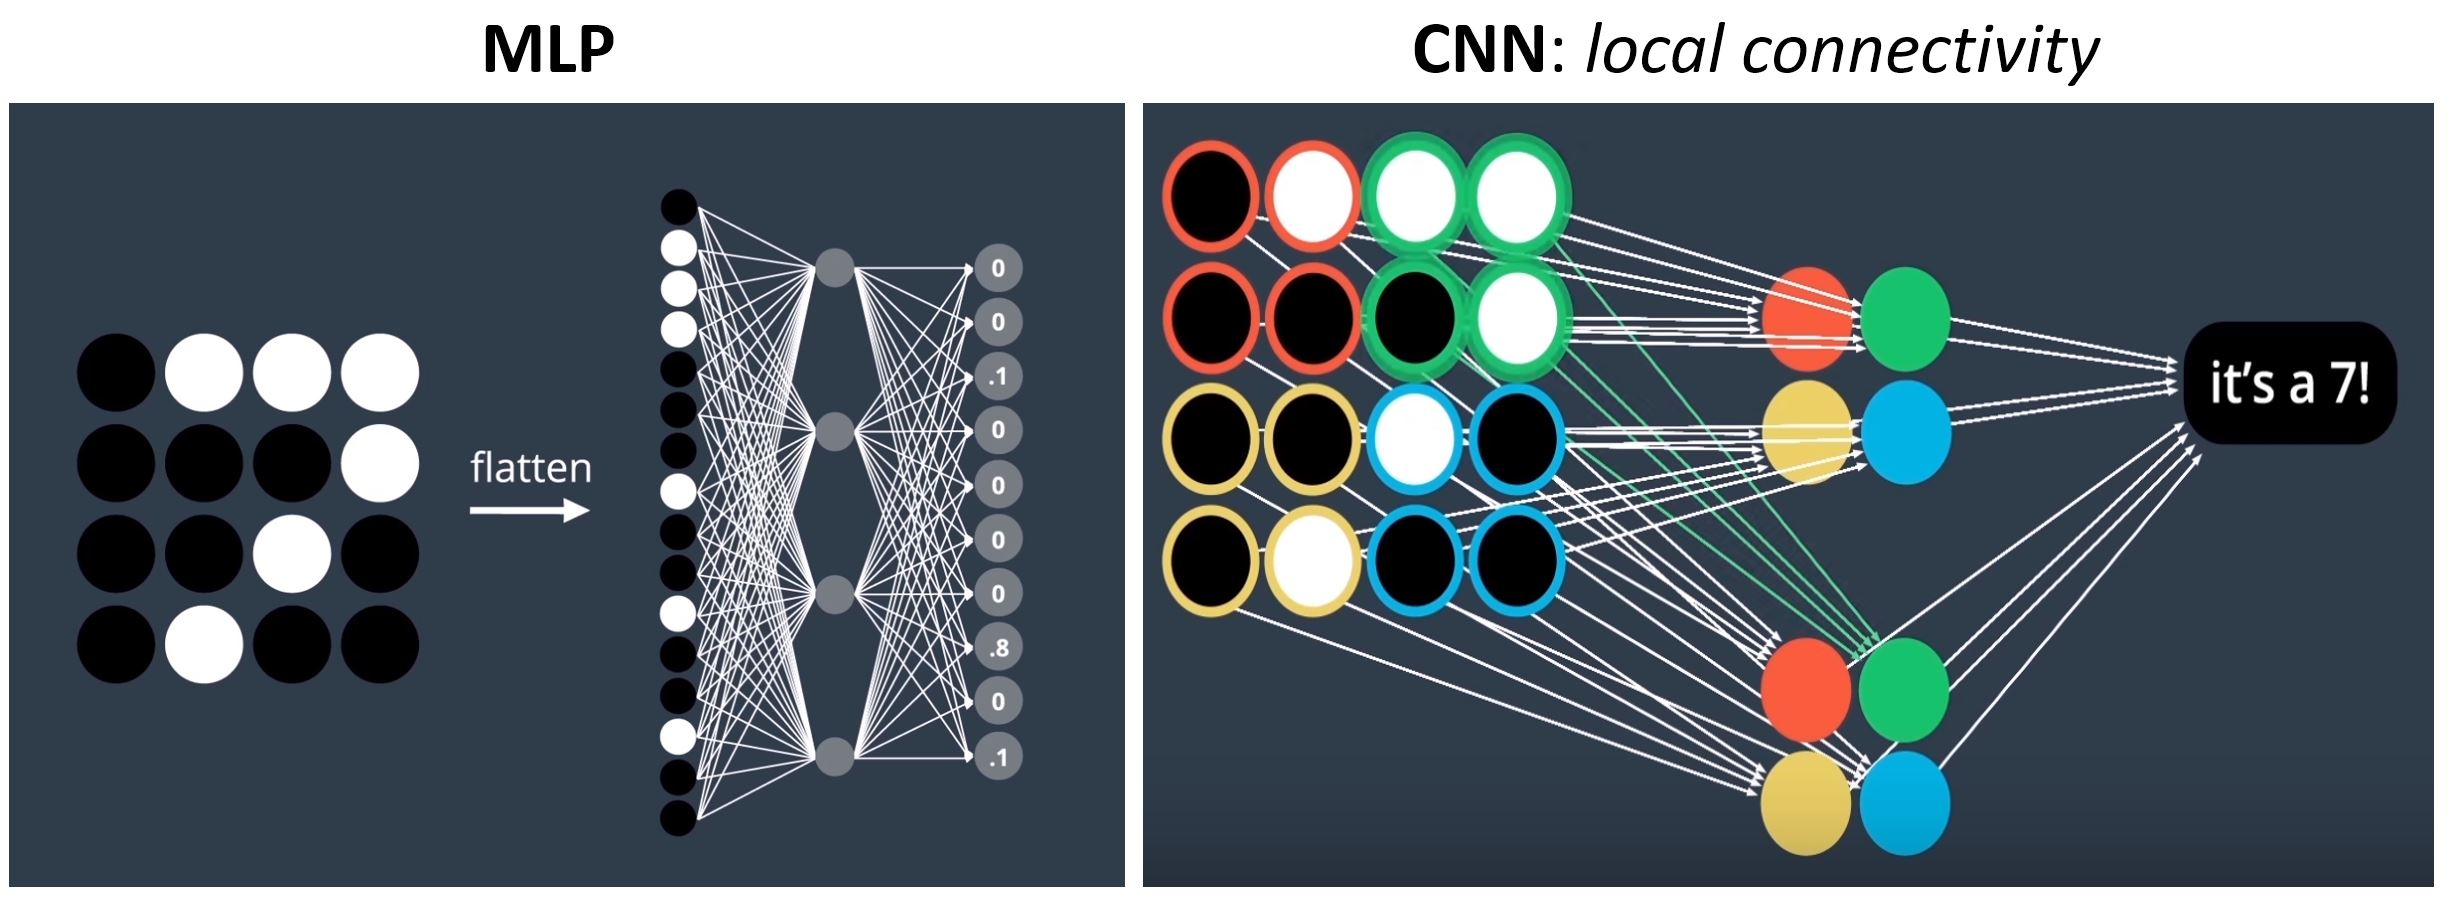
\includegraphics[width=0.8\textwidth]{pics/CNN_local_connectivity}
	\caption{MLPs vs CNNs: local connectivity} 
	\label{CNN_local_connectivity}
\end{figure}
%         --------------------------------------

%%%%%%%%%%%%%%%%%%%%%%%%%%%%%%%%%%%%%%%%%%%%%%%%%%%%%%
\subsubsection{Convolutional layers}
filter are convolved over the image...\\
filter weights are learned to minimise a loss function ...\\
%          --------   FIGURE: convolution layer 1  -----------
\begin{figure}[htbp] 
	\centering
	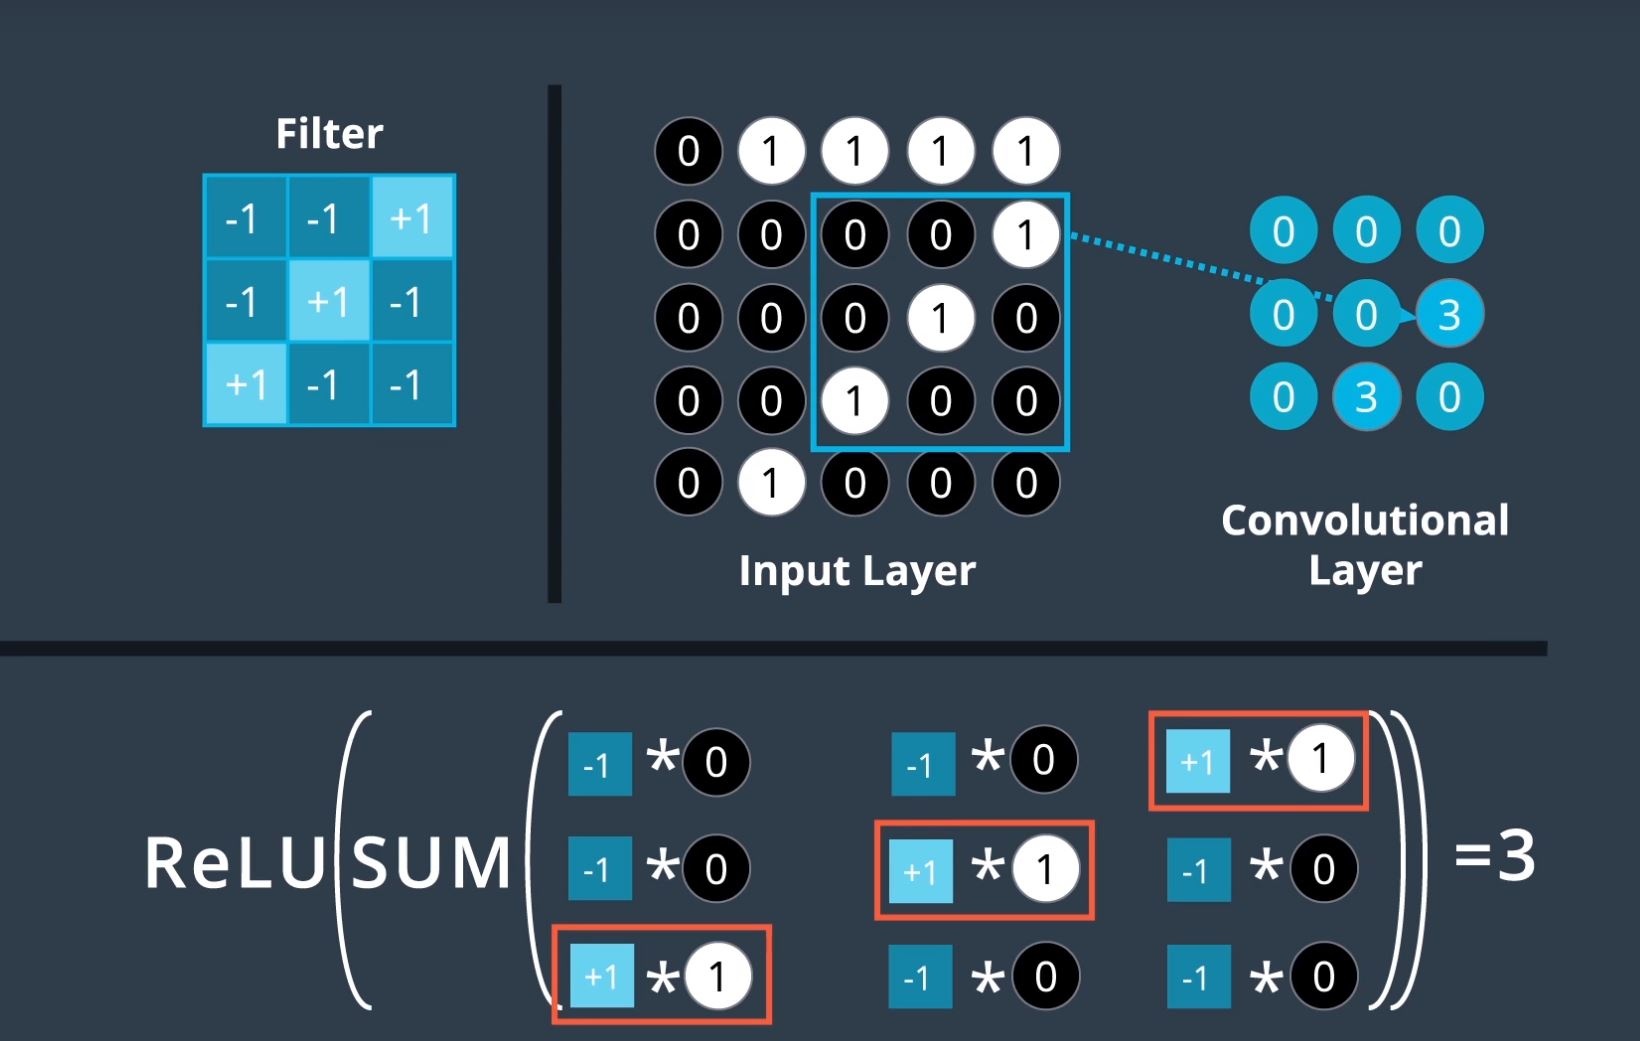
\includegraphics[width=0.7\textwidth]{pics/convolution_1}
	\caption{Convolution layer} 
	\label{convolution_1}
\end{figure}
%         --------------------------------------

Adding more filters (tens to hundreds to..) \\

Source for the 4 filters (or activation maps) code below is \href{https://github.com/udacity/aind2-cnn/blob/master/conv-visualization/conv_visualization.ipynb}{here} for more details.
\begin{lstlisting}
# define 4 filters
import numpy as np

filter_vals = np.array([[-1, -1, 1, 1], [-1, -1, 1, 1], 
				[-1, -1, 1, 1], [-1, -1, 1, 1]])

filter_1 = filter_vals
filter_2 = -filter_1
filter_3 = filter_1.T
filter_4 = -filter_3
filters = [filter_1, filter_2, filter_3, filter_4]


fromfrom  keras.models  import Sequential
from keras.layers.convolutional import Convolution2D
import matplotlib.cm as cm

# plot image
plt.imshow(small_img, cmap='gray')

# define a neural network with a single convolutional layer with one filter
model = Sequential()
model.add(Convolution2D(1, (4, 4), activation='relu', 
		input_shape=(small_img.shape[0], small_img.shape[1], 1)))
		# input_shape=(height, width, depth)

# apply convolutional filter and return output
def apply_filter(img, index, filter_list, ax):
	# set the weights of the filter in the convolutional layer to filter_list[i]
	model.layers[0].set_weights([np.reshape(filter_list[i], (4,4,1,1)), 
	np.array([0])])
	# plot the corresponding activation map
	ax.imshow(np.squeeze(model.predict(np.reshape(img, (1, img.shape[0], 
			img.shape[1], 1)))), cmap='gray')
\end{lstlisting}
In this car example, the first two filters identify the vertical lines (first the left line of the car), the other two horizontal lines.

We have a filter for each colour -  see fig \ref{convolution_2}
%          --------   FIGURE: convolution layer 2  -----------
\begin{figure}[htbp] 
	\centering
	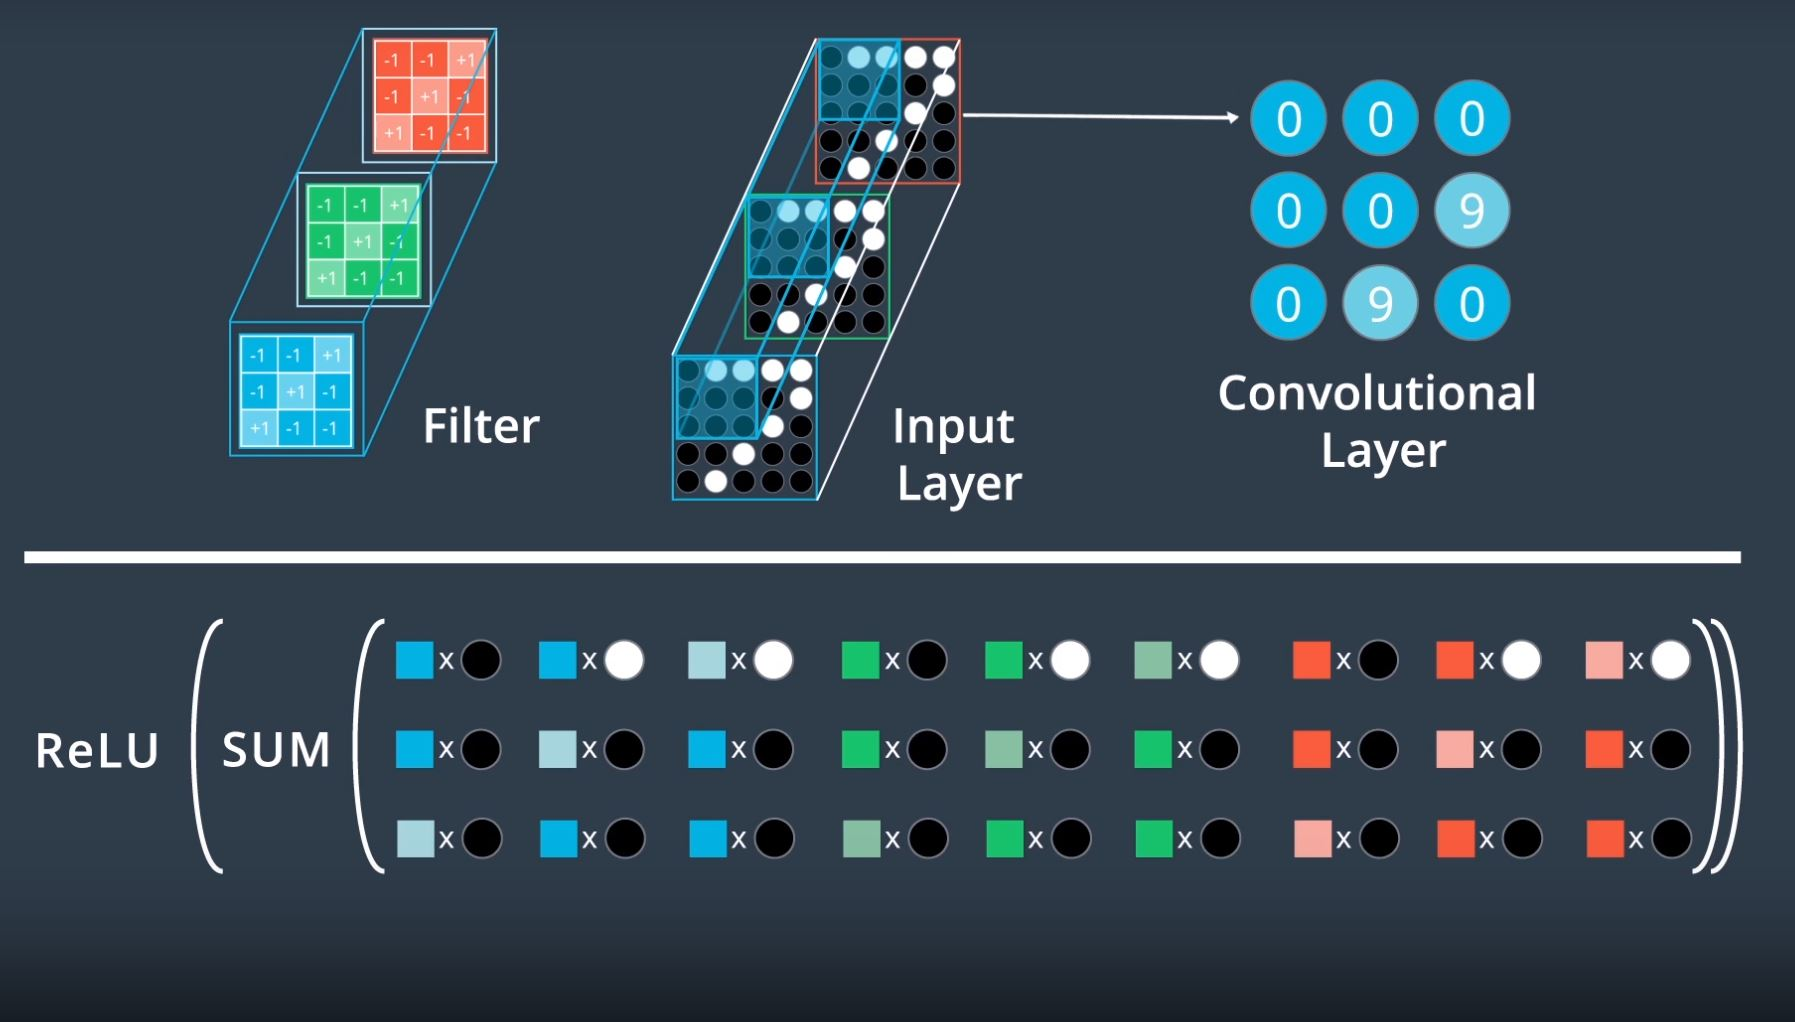
\includegraphics[width=0.7\textwidth]{pics/convolution_2}
	\caption{Convolution layer} 
	\label{convolution_2}
\end{figure}
%         --------------------------------------

Other hyperparameters of CCN (besides the required number and size of filters) are \textbf{stride}, amount of pixels that filter moves arounds (e.g. 1 pixel), and \textbf{padding} if filters strides outside (alternatively, ignore those nodes).


\begin{lstlisting}
# import library: Convolution2D is an alias of Conv2D
from keras.layers import Conv2D

Conv2D(filters, kernel_size, strides, padding, 
	  activation='relu', input_shape)
\end{lstlisting}
whose main arguments are:
\begin{itemize}
	\item filters (required)- The number of filters;
	\item kernel\_size (required) - an integer (tuple of 2 integers if different) specifying both the height and width of the convolution window (e.g. a square);
	\item input\_shape (required - if first layer after input) - Tuple specifying the height, width, and depth (in that order) of the input.
	\item strides (optional)- The stride of the convolution, default is 1.
	\item padding (optional) - One of 'valid' or 'same', default is 'valid'.
	\item activation (optional) - typically 'relu'. default is that no activation is applied; but strongly encouraged to add a ReLU.
\end{itemize}

The \textbf{number of parameters} in a convolutional layer depends on the values of (i) filters (the number of filters in the convolutional layer, $K$), (ii) kernel\_size (the height and width of the convolutional filters, $F$) and (iii) input\_shape (the depth of the previous layer, i.e. last value in the input\_shape tuple, $D_{in}$). \\
Since there are $F*F*D_{in}$ weights per filter and the convolutional layer is composed of K filters with one bias term per filter, then (the total number of weights is $K*F*F*D_{in}$ and) the number of parameters in the convolutional layer is given by $K*F*F*D_{in} + K$.

The \textbf{shape} (or spatial dimensions) in a convolutional layer depends on the values of (i) kernel\_size ($F$), (ii) input\_shape ($H_{in}$ and $W_{in}$ - height and with of the previous layer - respectively, the first and second value in the tuple), (iii) padding and (iv) stride ($S$):
\begin{itemize}
	\item If $padding = 'same'$, then the shape or spatial dimensions are 
	\begin{itemize}
		\item $height = ceil(float(H_{in}) / float(S))$ and
		\item $width = ceil(float(W_{in}) / float(S))$
	\end{itemize}
	\item if $padding = 'valid'$, then the spatial dimensions are
	\begin{itemize}
		\item $height = ceil(float(H_{in} - F + 1) / float(S))$  and
		\item $width = ceil(float(W_{in} - F + 1) / float(S))$
	\end{itemize}	
\end{itemize}
The output shape in Keras is a tuple of (batch size=None, height, width, depth), where depth is always equal to the number of filters $K$.

%%%%%%%%%%%%%%%%%%%%%%%%%%%%%%%%%%%%%%%%%%%%%%%%%%%%%%
\subsubsection{Pooling layers}
A third type of layers (besides Dense and Convolution ones) are pooling layers, that often take convolution layers as inputs - their goal is to reduce the number of parameters (and hence over-fitting) of convolutional layers.

There are two types of pooling layers: (i) \textbf{Max Pooling} Layer, for each feature map takes the max over a window (e.g. a square) striding e.g. 1 pixel at the time (generally half widht/height),  and (ii) \textbf{Global Average Pooling} Layer, taking the average over feature maps (getting a vector, even a smaller reduction  than max pooling). 

\begin{lstlisting}
from keras.models import Sequential
from keras.layers import MaxPooling2D

model = Sequential()
# MaxPooling2D(pool_size, strides, padding)
model.add(MaxPooling2D(pool_size=2, strides=2, input_shape=(100, 100, 15)))

model.summary()
\end{lstlisting}
where:
\begin{itemize}
	\item pool\_size (required)- Number specifying the height and width of the pooling window.
	\item strides (optional) - The vertical and horizontal stride, default is pool\_size.
	\item padding (optional) - either 'valid' or 'same', default set to 'valid'.
\end{itemize}

%%%%%%%%%%%%%%%%%%%%%%%%%%%%%%%%%%%%%%%%%%%%%%%%%%%%%%
\subsubsection*{CNNs for Image Classification}
Resizing images to same size (usually square, divisible by a power of 2 - e.g. 32x32)

From one input layer to a sequence to convulation layers (common settings: strides=1, which is default, padding='same' which is not the default, activaltion='relu'), max pooling layer follows one or two conv layers (common settings: both pool\_size and stride =2, padding default is ok - which halves spatial dimensions of conv layers).

\begin{lstlisting}
from keras.models import Sequential
from keras.layers import Conv2D, MaxPooling2D, Flatten, Dense

model = Sequential()

# 3 conv. layers, followed by max pooling ones
model.add(Conv2D(filters=16, kernel_size=2, padding='same', 
	activation='relu', input_shape=(32, 32, 3)))
model.add(MaxPooling2D(pool_size=2))
model.add(Conv2D(filters=32, kernel_size=2, padding='same', 
		activation='relu'))
model.add(MaxPooling2D(pool_size=2))
model.add(Conv2D(filters=64, kernel_size=2, padding='same', 
		activation='relu'))
model.add(MaxPooling2D(pool_size=2))

model.add(Flatten())
model.add(Dense(500, activation='relu'))

model.add(Dense(10, activation='softmax'))
\end{lstlisting}

Always add a ReLU activation function (most of times is the best in practice) to the Conv2D layers in your CNN. With the exception of the final layer in the network, Dense layers should also have a ReLU activation function. 

When constructing a network for classification, the final layer in the network should be a Dense layer with a softmax activation function. The number of nodes in the final layer should equal the total number of classes in the dataset.

For notebooks comparing between MLP and CNN on cifar10 (10 classes of tiny images, 32x32) \href{https://github.com/udacity/aind2-cnn/tree/master/cifar10-classification}{here}: from 40 to 66\% accuracy improvement. The Kaggle winner (a CNN) can be found \href{http://blog.kaggle.com/2015/01/02/cifar-10-competition-winners-interviews-with-dr-ben-graham-phil-culliton-zygmunt-zajac/}{here}.


%%%%%%%%%%%%%%%%%%%%%%%%%%%%%%%%%%%%%%%%%%%%%%%%%%%%%%
\subsubsection{Image Augmentation (Keras)}
We want our model to learn an \textbf{invariant representation} of the image/object, one that is not influenced by size (scale invariant), angle (rotation invariance), position  of the object in the image (translation invariance\footnote{Max Pooling layers add some translation invariance to the model - intuitevel, max function tend to stay the same around a neighbourhood area.}, e.g. squeezed to the left). One solution (which seems a bit like cheating) is to add some images with random rotation/translation/... to our dataset (this is called \textbf{data augmentation}), moreover that makes the model also less prone to over-fitting too - we say that we have \textit{augmented} our dataset.

The process starts by creating an \textbf{ImageDataGenerator} and then \textbf{fit} it on the data:
\begin{lstlisting}
from keras.preprocessing.image import ImageDataGenerator

# create and configure augmented image generator
datagen = ImageDataGenerator(featurewise_center=True,
	featurewise_std_normalization=True,
	rotation_range=90.,
	# randomly shift images horizontally (10% of total width)
	width_shift_range=0.1, 
	# randomly shift images vertically (10% of total height)
	height_shift_range=0.1,
	zoom_range=0.2))

# then fit to data
datagen.fit(x_train)
\end{lstlisting}

The data generator itself is an iterator, returning batches of image samples when requested. We can configure the batch size and prepare the data generator and get batches of images by calling the \textbf{flow} function. Finally - instead of calling the fit() function on our model - we must call the \textbf{fit\_generator()} function and pass in the data generator and the desired length of an epoch as well as the total number of epochs on which to train:
\begin{lstlisting}
# model architecture
model = Sequential()
model.add(Conv2D(filters=16, kernel_size=2, padding='same', 
	activation='relu', input_shape=(32, 32, 3)))
	model.add(MaxPooling2D(pool_size=2))
# etc. ... ...
model.add(Flatten())
model.add(Dense(10, activation='softmax'))

# compile model
model.compile(...)

# get batches
batch_size = 32
x_batch, y_batch = datagen.flow(x_train, y_train, batch_size=32)

# instead of fit, use fit_generator
_steps_per_epoch = x_train.shape[0] / batch_size

model.fit_generator(x_batch, y_batch, 
		steps_per_epoch=_steps_per_epoch,
		epochs=50)
\end{lstlisting}
where x\_train.shape[0] (or len(train)) corresponds to the number of \textit{unique} samples in the training dataset x\_train. By setting steps\_per\_epoch to this value, we ensure that the model sees x\_train.shape[0] augmented images in each epoch.

More details can be found on this \href{https://machinelearningmastery.com/image-augmentation-deep-learning-keras/}{blog post}.


%%%%%%%%%%%%%%%%%%%%%%%%%%%%%%%%%%%%%%%%%%%%%%%%%%%%%%
\subsubsection*{Groundbreaking CNN architectures}
\begin{itemize}
	\item \href{http://papers.nips.cc/paper/4824-imagenet-classification-with-deep-convolutional-neural-networks.pdf}{AlexNext of Toronto Uni}, 2012: introduced ReLU activation function and dropout (5 (11x11) convolutional layers)
	\item \href{https://arxiv.org/pdf/1409.1556.pdf}{VGGNet}, 2014 (Visual Geometry Group of Oxford) with either 16 or 19 (3x3) convolution layers, broken by 2x2 pooling layers, finished with 3 fully connected layers. Pioneered small windows (3x3) vs AlexNet larger ones.
	\item \href{https://arxiv.org/pdf/1512.03385v1.pdf}{ResNet}, 2015 (Microsoft) similarly VGG as idea of successive small layers (one was with 152 layers!), but with a solution to the vanishing gradient problem:	
\end{itemize}

To recap - according to the universal approximation theorem - given enough parameters  a feedforward network with a \textit{single} layer is sufficient to represent any function. However, the layer might be massive and network prone to overfitting - hence, since AlexNet, the common trend for network architecture is to go \textit{deeper} and deeper. Indeed, while AlexNet had only 5 convolutional layers, the VGG network had 19 layers and ResNet 152 (and up to 1k now). However, deep networks are hard to train because of the notorious \textit{vanishing gradient problem} - as the gradient is back-propagated to earlier layers, repeated multiplication may make the gradient infinitely small. As a result, as the network goes deeper, its performance gets saturated or even degraded. The core idea of ResNet is introducing a so-called \textit{identity shortcut connection} that skips one or more layers - more on \href{https://towardsdatascience.com/an-overview-of-resnet-and-its-variants-5281e2f56035}{here}.

You can access popular models for image classification already trained on ImageNet directly from \href{https://keras.io/applications/}{keras.applications}.

%%%%%%%%%%%%%%%%%%%%%%%%%%%%%%%%%%%%%%%%%%%%%%%%%%%%%%
\subsubsection{Transfer Learning}
Transfer learning involves taking a pre-trained neural network and adapting the neural network to a new, different data set.

Depending on both (i) the \textbf{size} of the new data set, and (ii) the \textbf{similarity} of the new data set to the original data set - there are 4 approaches for using transfer learning. In fig \ref{transfer_learning_cases}, we assume a generic pre-trained CNN (3 conv layers and 3 fully connected layers) to explain how to adjust the network for each case.
%          --------   FIGURE: Transfer learning: 4 cases  -----------
\begin{figure}[htbp] 
	\centering
	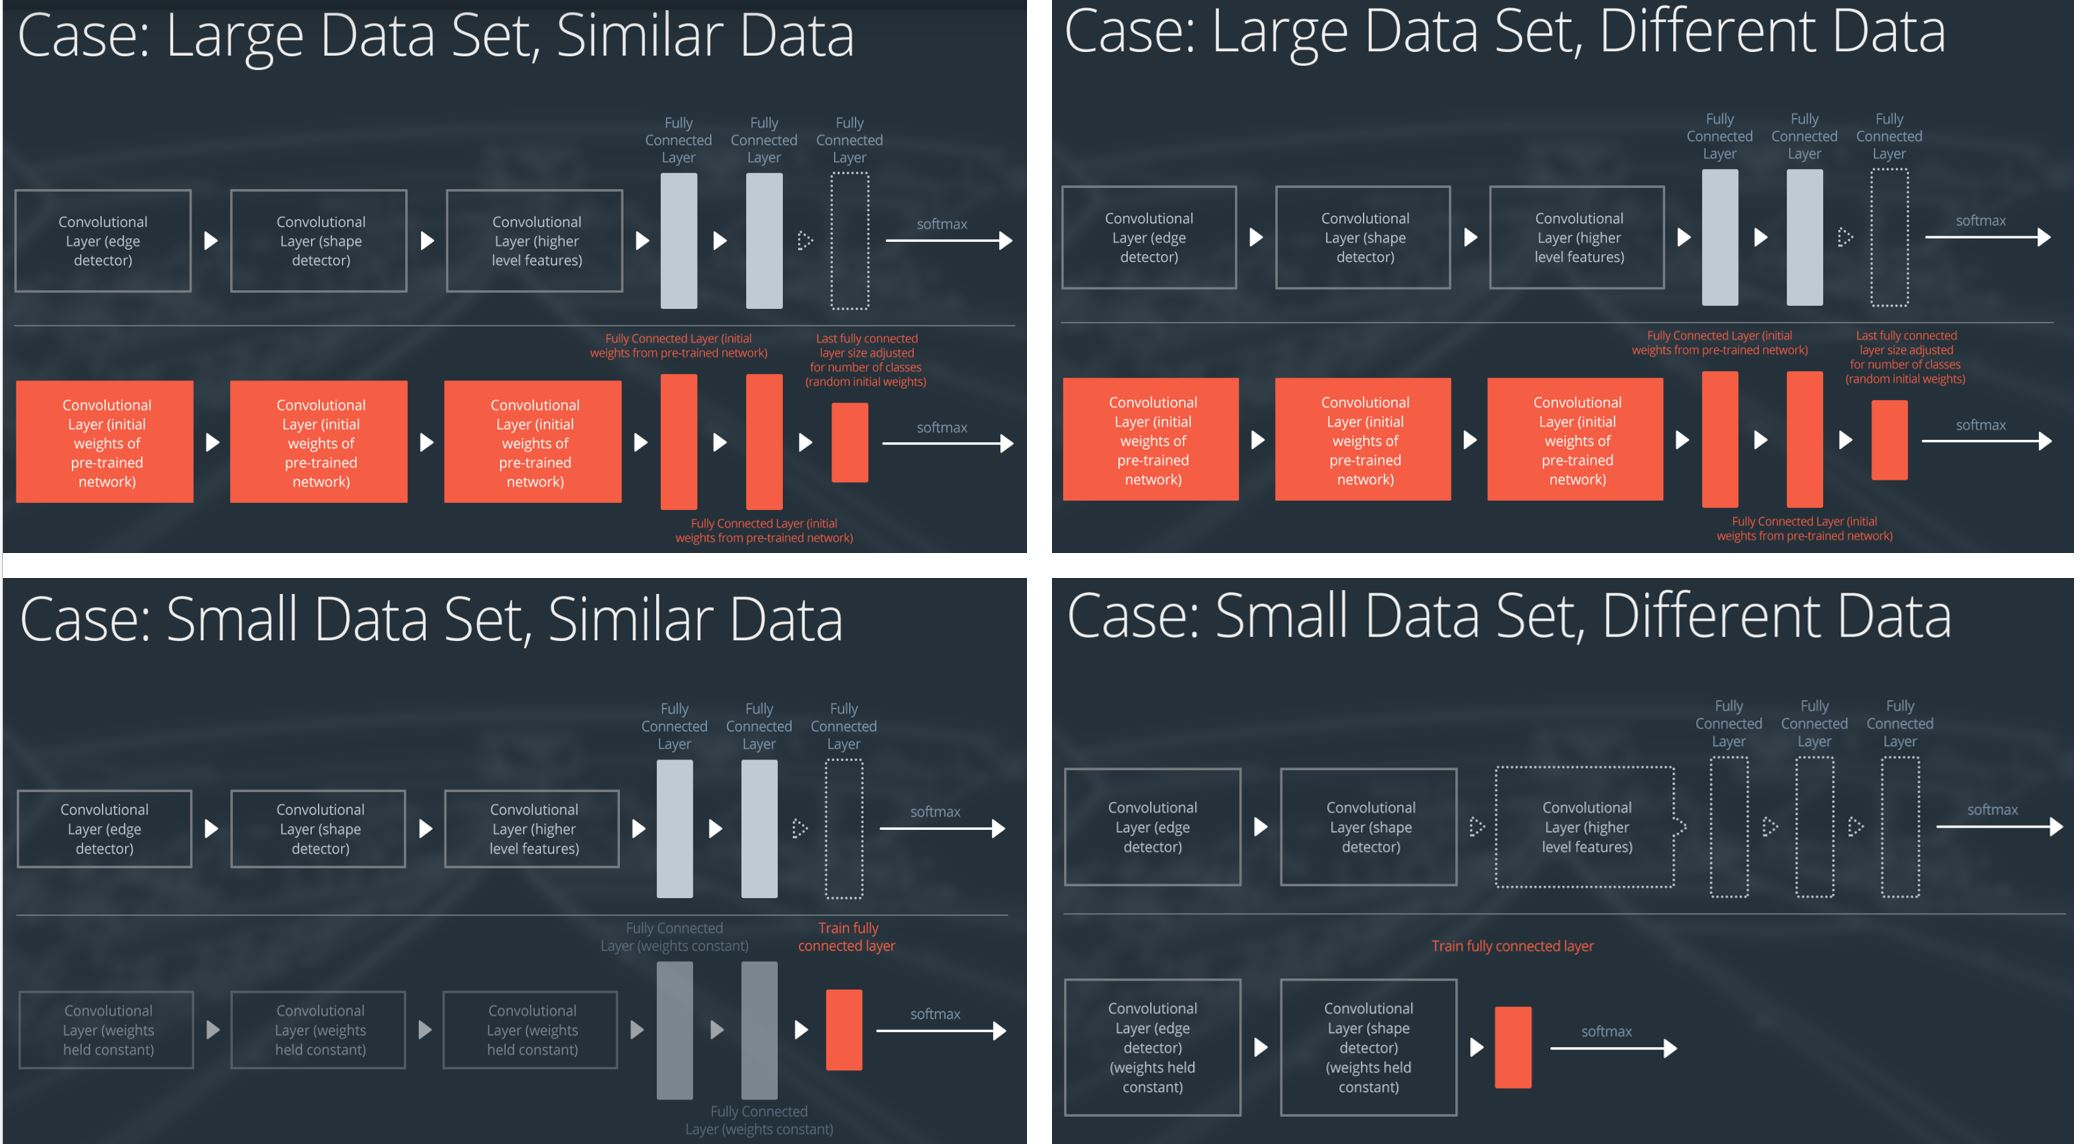
\includegraphics[width=0.95\textwidth]{pics/transfer_learning_cases}
	\caption{Transfer learning: 4 cases} 
	\label{transfer_learning_cases}
\end{figure}
%         --------------------------------------

A large data set might have one million images, a small data two-thousand images; the dividing line is somewhat subjective - but overfitting is a concern when using transfer learning with a small data set.

Regarding similarity, images of dogs and images of wolves would be considered similar since sharing common characteristics, but flower images datasets would be different from a data set of dog images.

If the new data set is \textbf{small and similar} to the original training data: (i) slice off the end of the neural network, (ii) add a new fully connected layer that matches the number of classes in the new data set, (iii)
randomize the weights of the new fully connected layer, freeze all the weights from the pre-trained network (iv) train the network to update the weights of the new fully connected layer. To avoid overfitting on the small data set, the weights of the original network will be held constant rather than re-training the weights. Since data sets are similar, images from each data set will have similar higher level features, therefore most or all of the pre-trained neural network layers should be kept.

If the new data set is \textbf{small and different} from the original training data: (i) slice off most of the pre-trained layers near the beginning of the network, (ii) add to the remaining pre-trained layers a new fully connected layer that matches the number of classes in the new data set, (iii) randomize the weights of the new fully connected layer, freeze all the weights from the pre-trained network, (iv) train the network to update the weights of the new fully connected layer. Because the data set is small, overfitting is still a concern: the weights of the original neural network will be held constant, like in the previous case - but since original and new data set do not share higher level features, the new network will only use the layers containing lower level features.

If the new data set is \textbf{large and similar} to the original training data: (i) remove the last fully connected layer and replace with a layer matching the number of classes in the new data set (ii) randomly initialize the weights in the new fully connected layer, (iii) initialize the rest of the weights using the pre-trained weights, (iv) re-train the \textit{entire} neural network. Overfitting is not as much of a concern, therefore, you can re-train all of the weights. Also since datasets share higher level features, the entire neural network is used as well.

If the new data set is \textbf{large and different} from the original training data: (i) remove the last fully connected layer and replace with a layer matching the number of classes in the new data set, (ii) retrain the network from scratch with randomly initialized weights, (iii) alternatively, you could just use the same strategy as the "large and similar" data case above. Even though the data set is different from the training data, initializing the weights from the pre-trained network might make training faster. So this case is exactly the same as the case with a large, similar data set.

%%%%%%%%%%%%%%%%%%%%%%%%%%%%%%%%%%%%%%%%%%%%%%%%%%%%%%
\subsubsection*{Transfer Learning in Keras}
TO BE COMPLETED
read the following blog post (particularly the fine-tuning):  \url{https://blog.keras.io/building-powerful-image-classification-models-using-very-little-data.html}

%%%%%%%%%%%%%%%%%%%%%%%%%%%%%%%%%%%%%%%%%%%%%%%%%%%%%%
%	MISCELLANEOUS LEARNING
%%%%%%%%%%%%%%%%%%%%%%%%%%%%%%%%%%%%%%%%%%%%%%%%%%%%%%
\section{Miscellaneous}

%%%%%%%%%%%%%%%%%%%%%%%%%%%%%%%%%%%%%%%%%%%%%%%%%%%%%%
\subsection{Recommender systems}
To be completed
%%%%%%%%%%%%%%%%%%%%%%%%%%%%%%%%%%%%%%%%%%%%%%%%%%%%%%
\subsection{Natural Language Processing (NLTK)}
To be completed
%%%%%%%%%%%%%%%%%%%%%%%%%%%%%%%%%%%%%%%%%%%%%%%%%%%%%%
\subsection{Big Data (Spark)}
To be completed


%%%%%%%%%%%%%%%%%%%%%%%%%%%%%%%%%%%%%%%%%%%%%%%%%%%%%%
%	APPENDIX	%%%%%%%%%%%%%%%%%%%%%%%%%%%%%%%%%%%%%%
%%%%%%%%%%%%%%%%%%%%%%%%%%%%%%%%%%%%%%%%%%%%%%%%%%%%%%
\clearpage
\appendix
%Note that this is quite similar to Equation~\eqref{eq:eqA} in Appendix~\ref{sec:app1}.
%%%%%%%%%%%%%%%%%%%%%%%%%%%%%%%%%%%%%%%%%%%%%%%%%%%%%%%%%%%%%%%%%%%%%%%%%%%
%% 					Appendix 1
\section{Miscellaneous}\label{sec:app1}
Some interesting, but not directly related topics are reported here.

\begin{lstlisting}
from sklearn.metrics import make_scorer
from sklearn.tree import DecisionTreeRegressor
from sklearn.model_selection import GridSearchCV

def fit_model(X, y):
   """ Performs grid search over the 'max_depth' parameter for a 
   decision tree regressor trained on the input data [X, y]. """

   # Create cross-validation sets from the training data
   cv_sets = ShuffleSplit(n_splits = 10, test_size = 0.20, random_state = 0)

   # Create a decision tree regressor object
   regressor = DecisionTreeRegressor()

   # Create a dictionary for the parameter 'max_depth' with a range from 1 to 10
   params = {'max_depth':[i for i in range(1,11)]}

   # Transform 'performance_metric' into a scoring function using 'make_scorer' 
   scoring_fnc = make_scorer(performance_metric)

   # Create the grid search cv object --> GridSearchCV()
   # (estimator, param_grid, scoring, cv) 
   grid = GridSearchCV(regressor, param_grid=params, scoring=scoring_fnc, cv=cv_sets)

   # Fit the grid search object to the data to compute the optimal model
   grid = grid.fit(X, y)

   # Return the optimal model after fitting the data
   return grid.best_estimator_
\end{lstlisting}


%          --------   Bayesain quiz  -----------
\begin{figure}[htbp] 
	\centering
	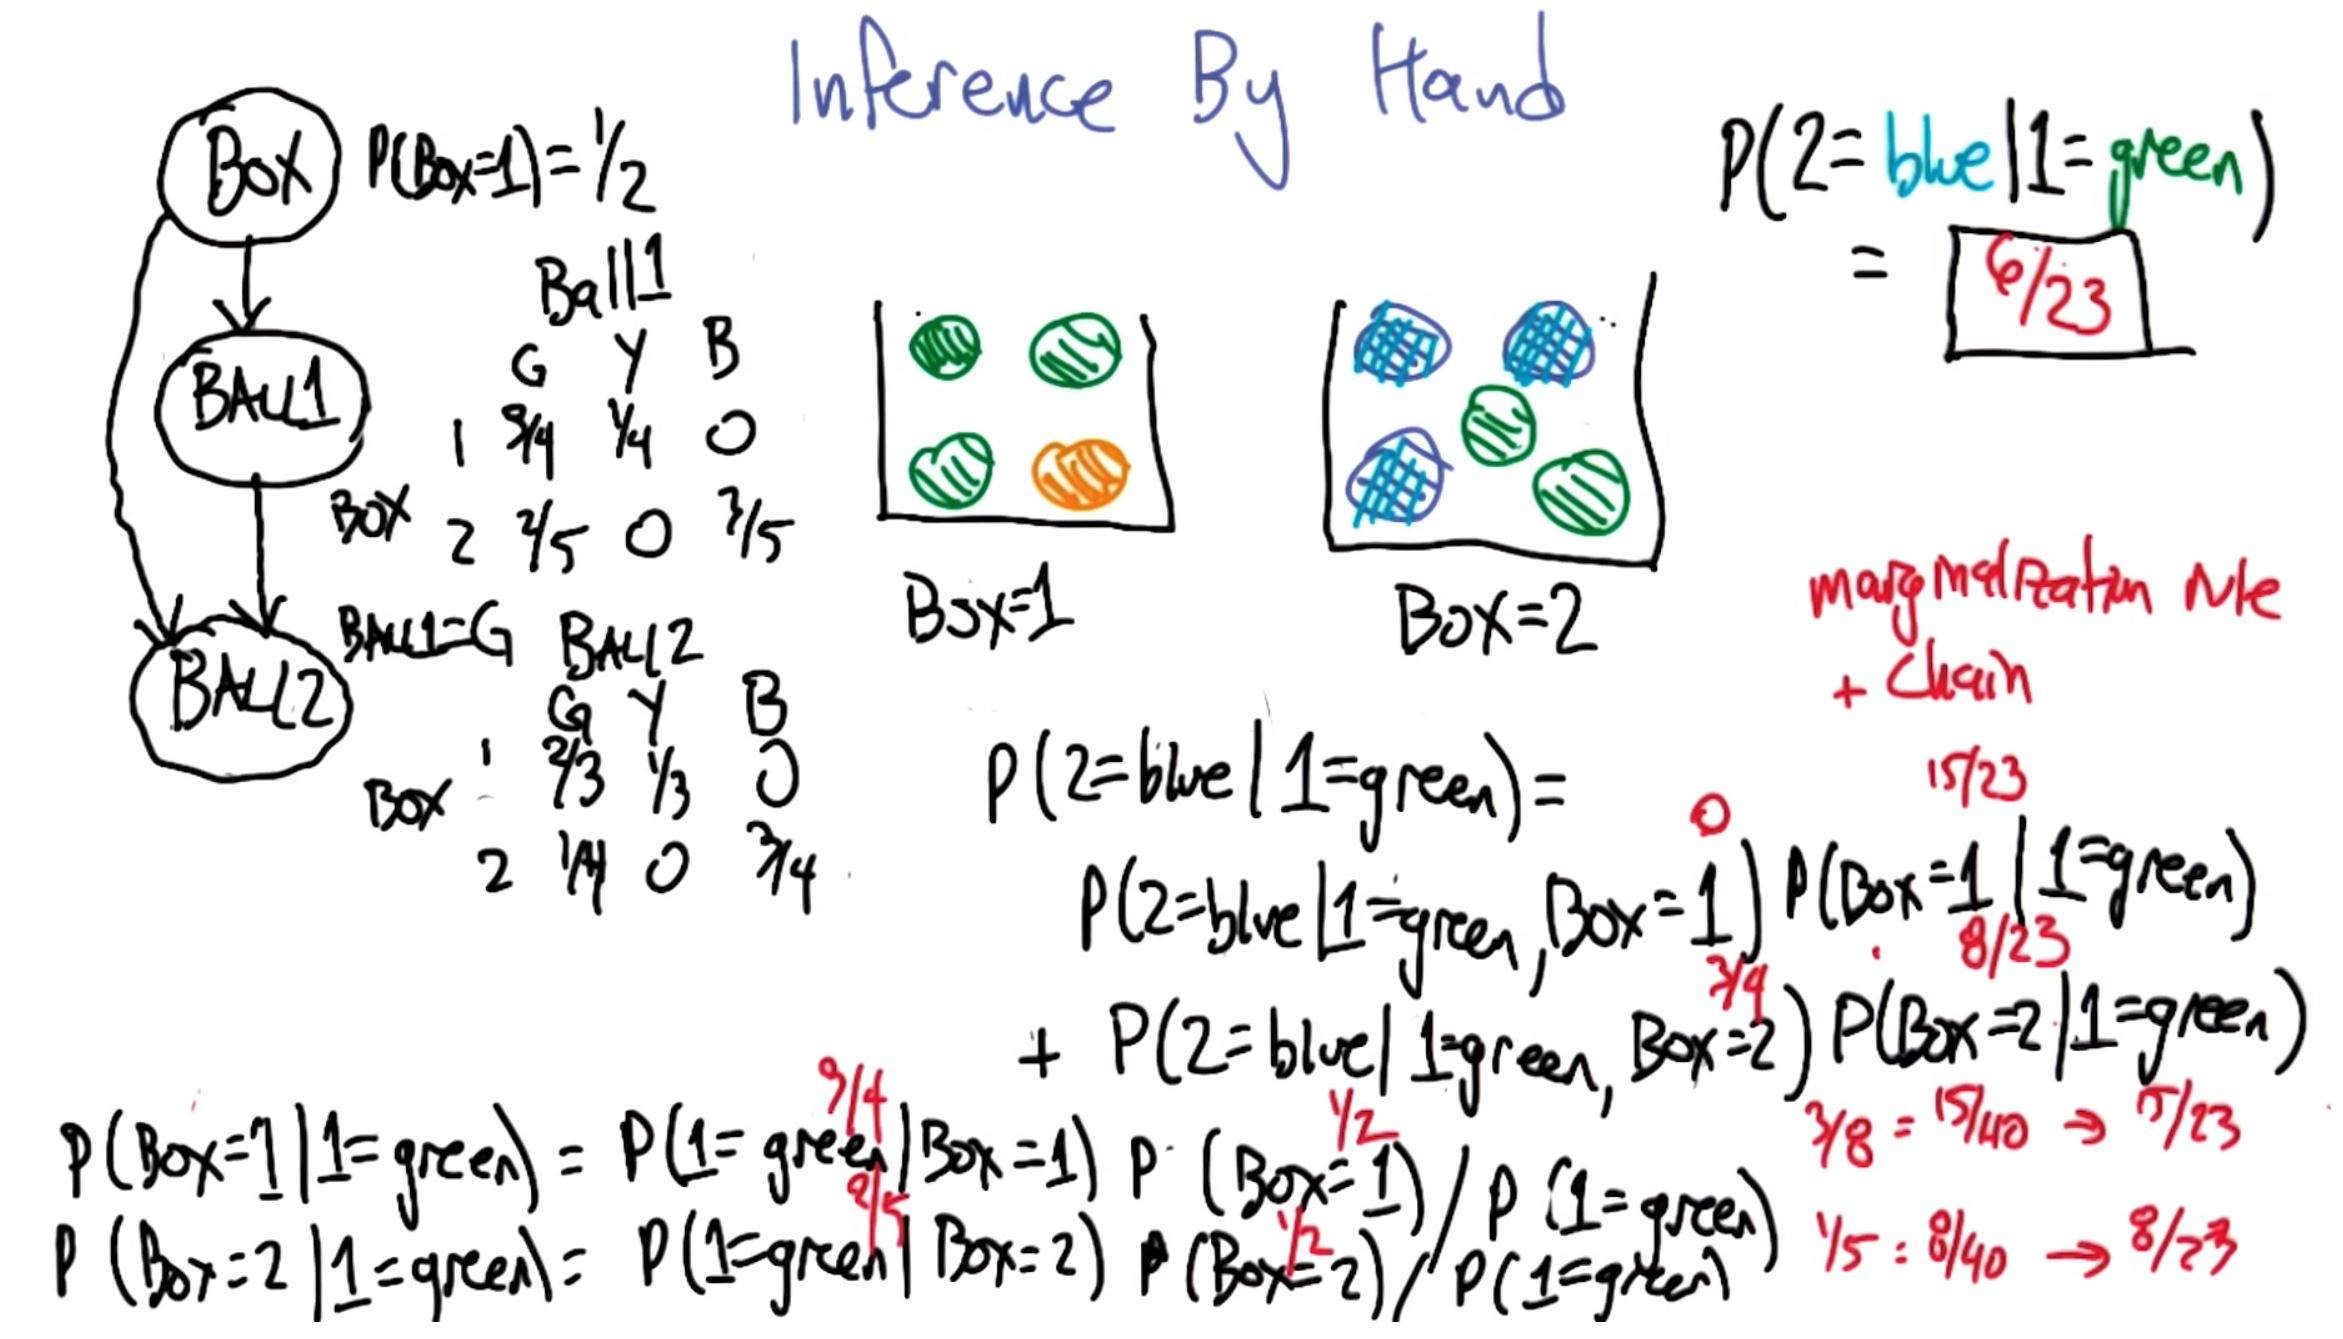
\includegraphics[width=0.9\textwidth]{pics/quiz_bayes}
	\caption{Bayes quiz} 
	\label{bayes_quiz}
\end{figure}
%         --------------------------------------


%%%%%%%%%%%%%%%%%%%%%%%%%%%%%%%%%%%%%%%%%%%%%%%%%%%%%%
\subsection{MLP on MNIST} \label{mln_on_mnist}
The MNIST Database contains 70k hand-written digits - probably the most famous database in machine learning. 

Each image is a 28x28 pixel matrix, so we first need to flatten the data if we use MLP, i.e. from matrix (digits of black '0', grey '114' and white '255') to a vectors (contrary to CNNs). Main part of the code below is part $6$.

\begin{lstlisting}
# 1. Load MNIST Database
from keras.datasets import mnist

# use Keras to import pre-shuffled MNIST database
(X_train, y_train), (X_test, y_test) = mnist.load_data()

print("The MNIST database has a training set of %d examples." % len(X_train))
print("The MNIST database has a test set of %d examples." % len(X_test))

# 2. Visualise first 6 training images
import matplotlib.pyplot as plt
%matplotlib inline
import matplotlib.cm as cm
import numpy as np

# plot first six training images
fig = plt.figure(figsize=(20,20))
for i in range(6):
	ax = fig.add_subplot(1, 6, i+1, xticks=[], yticks=[])
	ax.imshow(X_train[i], cmap='gray')
	ax.set_title(str(y_train[i]))

# 3. View an image in more details
def visualize_input(img, ax):
	ax.imshow(img, cmap='gray')
	width, height = img.shape
	thresh = img.max()/2.5
	for x in range(width):
		for y in range(height):
			ax.annotate(str(round(img[x][y],2)), xy=(y,x),
			horizontalalignment='center',
			verticalalignment='center',
			color='white' if img[x][y]<thresh else 'black')

fig = plt.figure(figsize = (12,12)) 
ax = fig.add_subplot(111)
visualize_input(X_train[0], ax)

# 4. Rescale images dividing each pixel by 255
# rescale [0,255] to lie in [0,1]
X_train = X_train.astype('float32')/255
X_test = X_test.astype('float32')/255 

# 5. Encode Categorical Integer Labels Using a One-Hot Scheme
from keras.utils import np_utils

# print first ten (integer-valued) training labels
print('Integer-valued labels:')
print(y_train[:10])

# one-hot encode the labels 
# (from 10 labels to 10 vectors of zeroes bar 1)
y_train = np_utils.to_categorical(y_train, 10)
y_test = np_utils.to_categorical(y_test, 10)

# print first ten (one-hot) training labels
print('One-hot labels:')
print(y_train[:10])

# 6. Define Model Architecture, compile & train
from keras.models import Sequential
from keras.layers import Dense, Dropout, Flatten

# define the model
model = Sequential()

# from matrix to a single vector: 784 nodes
# contrary to CNNs built for multi-dim data
model.add(Flatten(input_shape=X_train.shape[1:]))

model.add(Dense(512, activation='relu'))
model.add(Dropout(0.2))

model.add(Dense(512, activation='relu'))
model.add(Dropout(0.2))

# 10 nodes - one for each digit
model.add(Dense(10, activation='softmax'))

# summarize the model
model.summary()

# compile the model
model.compile(loss='categorical_crossentropy', 
		optimizer='rmsprop', 
		metrics=['accuracy'])

from keras.callbacks import ModelCheckpoint   

# there are many CALLABACKs, e.g. 
# checkpointer which saves model after every epoch,
# in case of system failure for long-running processes
checkpointer = ModelCheckpoint(filepath='mnist.model.best.hdf5', 
		verbose=1, save_best_only=True)

## another example of CALLABACK which stops training 
## when a monitored quantity stops improving
# keras.callbacks.EarlyStopping(monitor='val_loss', min_delta=0,
#                              patience=0, verbose=0, mode='auto')

# train the model
# note "validation_split=0.2": 20% of final data 
# removed and used as validation set
# if loss decreases then model is good
hist = model.fit(X_train, y_train, 
		batch_size=128, epochs=10,
		validation_split=0.2, 
		callbacks=[checkpointer],
		verbose=1, shuffle=True)

# 7 Evaluate
# load the weights that yielded the best validation accuracy
model.load_weights('mnist.model.best.hdf5')

# print test accuracy
score = model.evaluate(X_test, y_test, verbose=0)
accuracy = 100*score[1]
print('Test accuracy: %.4f%%' % accuracy)

# get predictions on the test set
y_hat = model.predict(X_test)
\end{lstlisting}

%%%%%%%%%%%%%%%%%%%%%%%%%%%%%%%%%%%%%%%%%%%%%%%%%%%%%%
\subsection{Gradient Descent} \label{gradient_descent}
There are three variants of gradient descent, which differ in how much data we use to compute the gradient of the objective function - see this \href{http://ruder.io/optimizing-gradient-descent/}{blog} for more details. 

\subsubsection*{Batch Gradient Descent}
Vanilla gradient descent, aka batch gradient descent, computes the gradient of the cost function w.r.t. to the parameters θ for the \textit{entire} training dataset:
\[ \theta = \theta - \eta \nabla_{\theta} J(\theta)
\]
As we need to calculate the gradients for the whole dataset to perform just one update, batch gradient descent can be very slow and is intractable for datasets that don't fit in memory. Batch gradient descent also doesn't allow us to update our model online, i.e. with new examples on-the-fly.

In  code:
\begin{lstlisting}
for i in range(nb_epochs):
	# gradient on entire data
	params_grad = evaluate_gradient(loss_function, data, params)
	params = params - learning_rate * params_grad
\end{lstlisting}
%

\subsubsection*{Stochastic Gradient Descent}
Stochastic gradient descent (SGD) in contrast performs a parameter update for \textit{each training example} $x^{(i)}$ and label $y^{(i)}$:
\[ \theta = \theta - \eta \nabla_{\theta} J(\theta; x^{(i)}, y^{(i)})
\]
Batch gradient descent performs redundant computations for large datasets. SGD does away with this redundancy by performing one update at a time. It is therefore usually much faster and can also be used to learn online. In addition, SGD's fluctuation enables it to jump to new and potentially better local minima (learning rate needs to be small ot avoid overshooting).

In  code:
\begin{lstlisting}
for i in range(nb_epochs):
	np.random.shuffle(data)	
	for example in data:
		# gradient on each training example
		params_grad = evaluate_gradient(loss_function, example, params)
		params = params - learning_rate * params_grad
\end{lstlisting}
%

\subsubsection*{Mini-batch Gradient Descent}
Mini-batch gradient descent finally takes the best of both worlds and performs an update for every mini-batch of $n$ training examples::
\[ \theta = \theta - \eta \nabla_{\theta} J(\theta; x^{(i:i+n)}, y^{(i:i+n)})
\]
This way, it a) reduces the variance of the parameter updates (more stable convergence) and b) can make use of highly optimized matrix optimizations common to state-of-the-art deep learning libraries. Common mini-batch sizes range between 50 and 256, but can vary for different applications. Mini-batch gradient descent is typically the algorithm of choice when training a neural network.

In  code:
\begin{lstlisting}
for i in range(nb_epochs):
	np.random.shuffle(data)
	for batch in get_batches(data, batch_size=50):
		# gradient mini-batch
		params_grad = evaluate_gradient(loss_function, batch, params)
		params = params - learning_rate * params_grad
\end{lstlisting}


\clearpage

%%%%%%%%%%%%%%%%%%%%%%%%%%%%%%%%%%%%%%%%%%%%%%%%%
% Bibliography.
%%%%%%%%%%%%%%%%%%%%%%%%%%%%%%%%%%%%%%%%%%%%%%%%%

%% adds the bibliography to the table of contents: usato per la tesi
%  \addcontentsline{toc}{chapter} 
%  {\protect\numberline{Bibliography\hspace{-96pt}}} 

%% uncomment almeno le due seguenti
%  \bibliographystyle{jfe} % stile della biblio
%  \bibliography{allrefs} % nome del file dove raccogliere le bibliografie

\clearpage

% \ 
% \vfill
% \begin{figure}[!htb]
%  \centerline{\includegraphics[width=7in]{pics/Figure1}}
%  \caption{Structure of model. Capital can be invested in a bank sector and an equity sector. An intermediary has the expertise to reallocate capital between the sectors andto monitor bank capital against bank crashes.} \label{fig:0}
%  \end{figure}
% \vfill
% \ 
	
\end{document}




% --- esempio di come si include la bibliografia ---
% Among the interesting books and papers I have read in the course of this work is 
% Halzen and Martin's {\it Quarks and Leptons}\,\cite{Halzen:1984mc}, and the paper {\it Can
% one probe the structure of the pomeron?} by Ellis and
% Ross,\cite{Ellis:1996cg}.

% or for the "journal of finance" kind of style, we can also have the following options: \citeyear{fama/french:88-jpe} produces (1988b), and \citename{fama/french:88-jpe} produces Fama and French. 

% HYPERREF
% \url{http://www.wikibooks.org}
%  \href{http://www.wikibooks.org}{Wikibooks home}
% Both point at the same page, but in the first case the URL will be shown, while in the second case the URL will be hidden. Note that, if you print your document, the link stored using \href will not be shown anywhere in the document.


% IMPORTANT:
% --- When processing the file, you need to do: LATEX filename, BIBTEX filename, LATEX filename, LATEX filename ---